\documentclass{article}
\usepackage{graphicx}
\usepackage{amsmath}
\usepackage{float}
\usepackage[utf8]{inputenc}
\newcommand*\xor{\mathbin{\oplus}}
\def\code#1{\texttt{#1}}
\begin{document}

\noindent Phillip Trent
\\ESE 370
\\Optimization of 16-bit Adder
\\\section{The Objective}
The goal is to optimize a single bit slice of a ripple carry adder in such a way as to minimize the delay of a 16b adder. The single bit slice waveform is shown in Figure \ref{fig:waveform1} with the sum output $S$ and carry out labeled $Cout$.

\begin{figure}[H]
  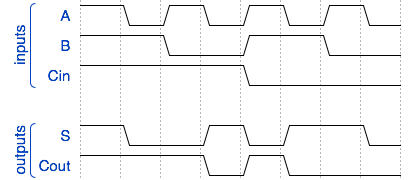
\includegraphics[width=\linewidth]{baseline_screenshots/wavedrom.png}
  \caption{Target waveform for single bit slice}
  \label{fig:waveform1}
\end{figure}

\section{Baseline Design}
For the baseline design, I used the following equations for sum and carry out logic:
$$S = A \xor B \xor Cin$$
$$Cout = AB + ACin + BCin$$
\\I created a 3-input CMOS XNOR gate. The schematic for which is shown in Figure \ref{fig:3inputnor} and then inverted the output for the sum as shown in Figure \ref{fig:baselinesch}. The carry out was taken directly from the equation above and translated into CMOS logic. I did not use a gate structure because the logic is simple enough to create a custom CMOS design. \pagebreak

\begin{figure}[H]
  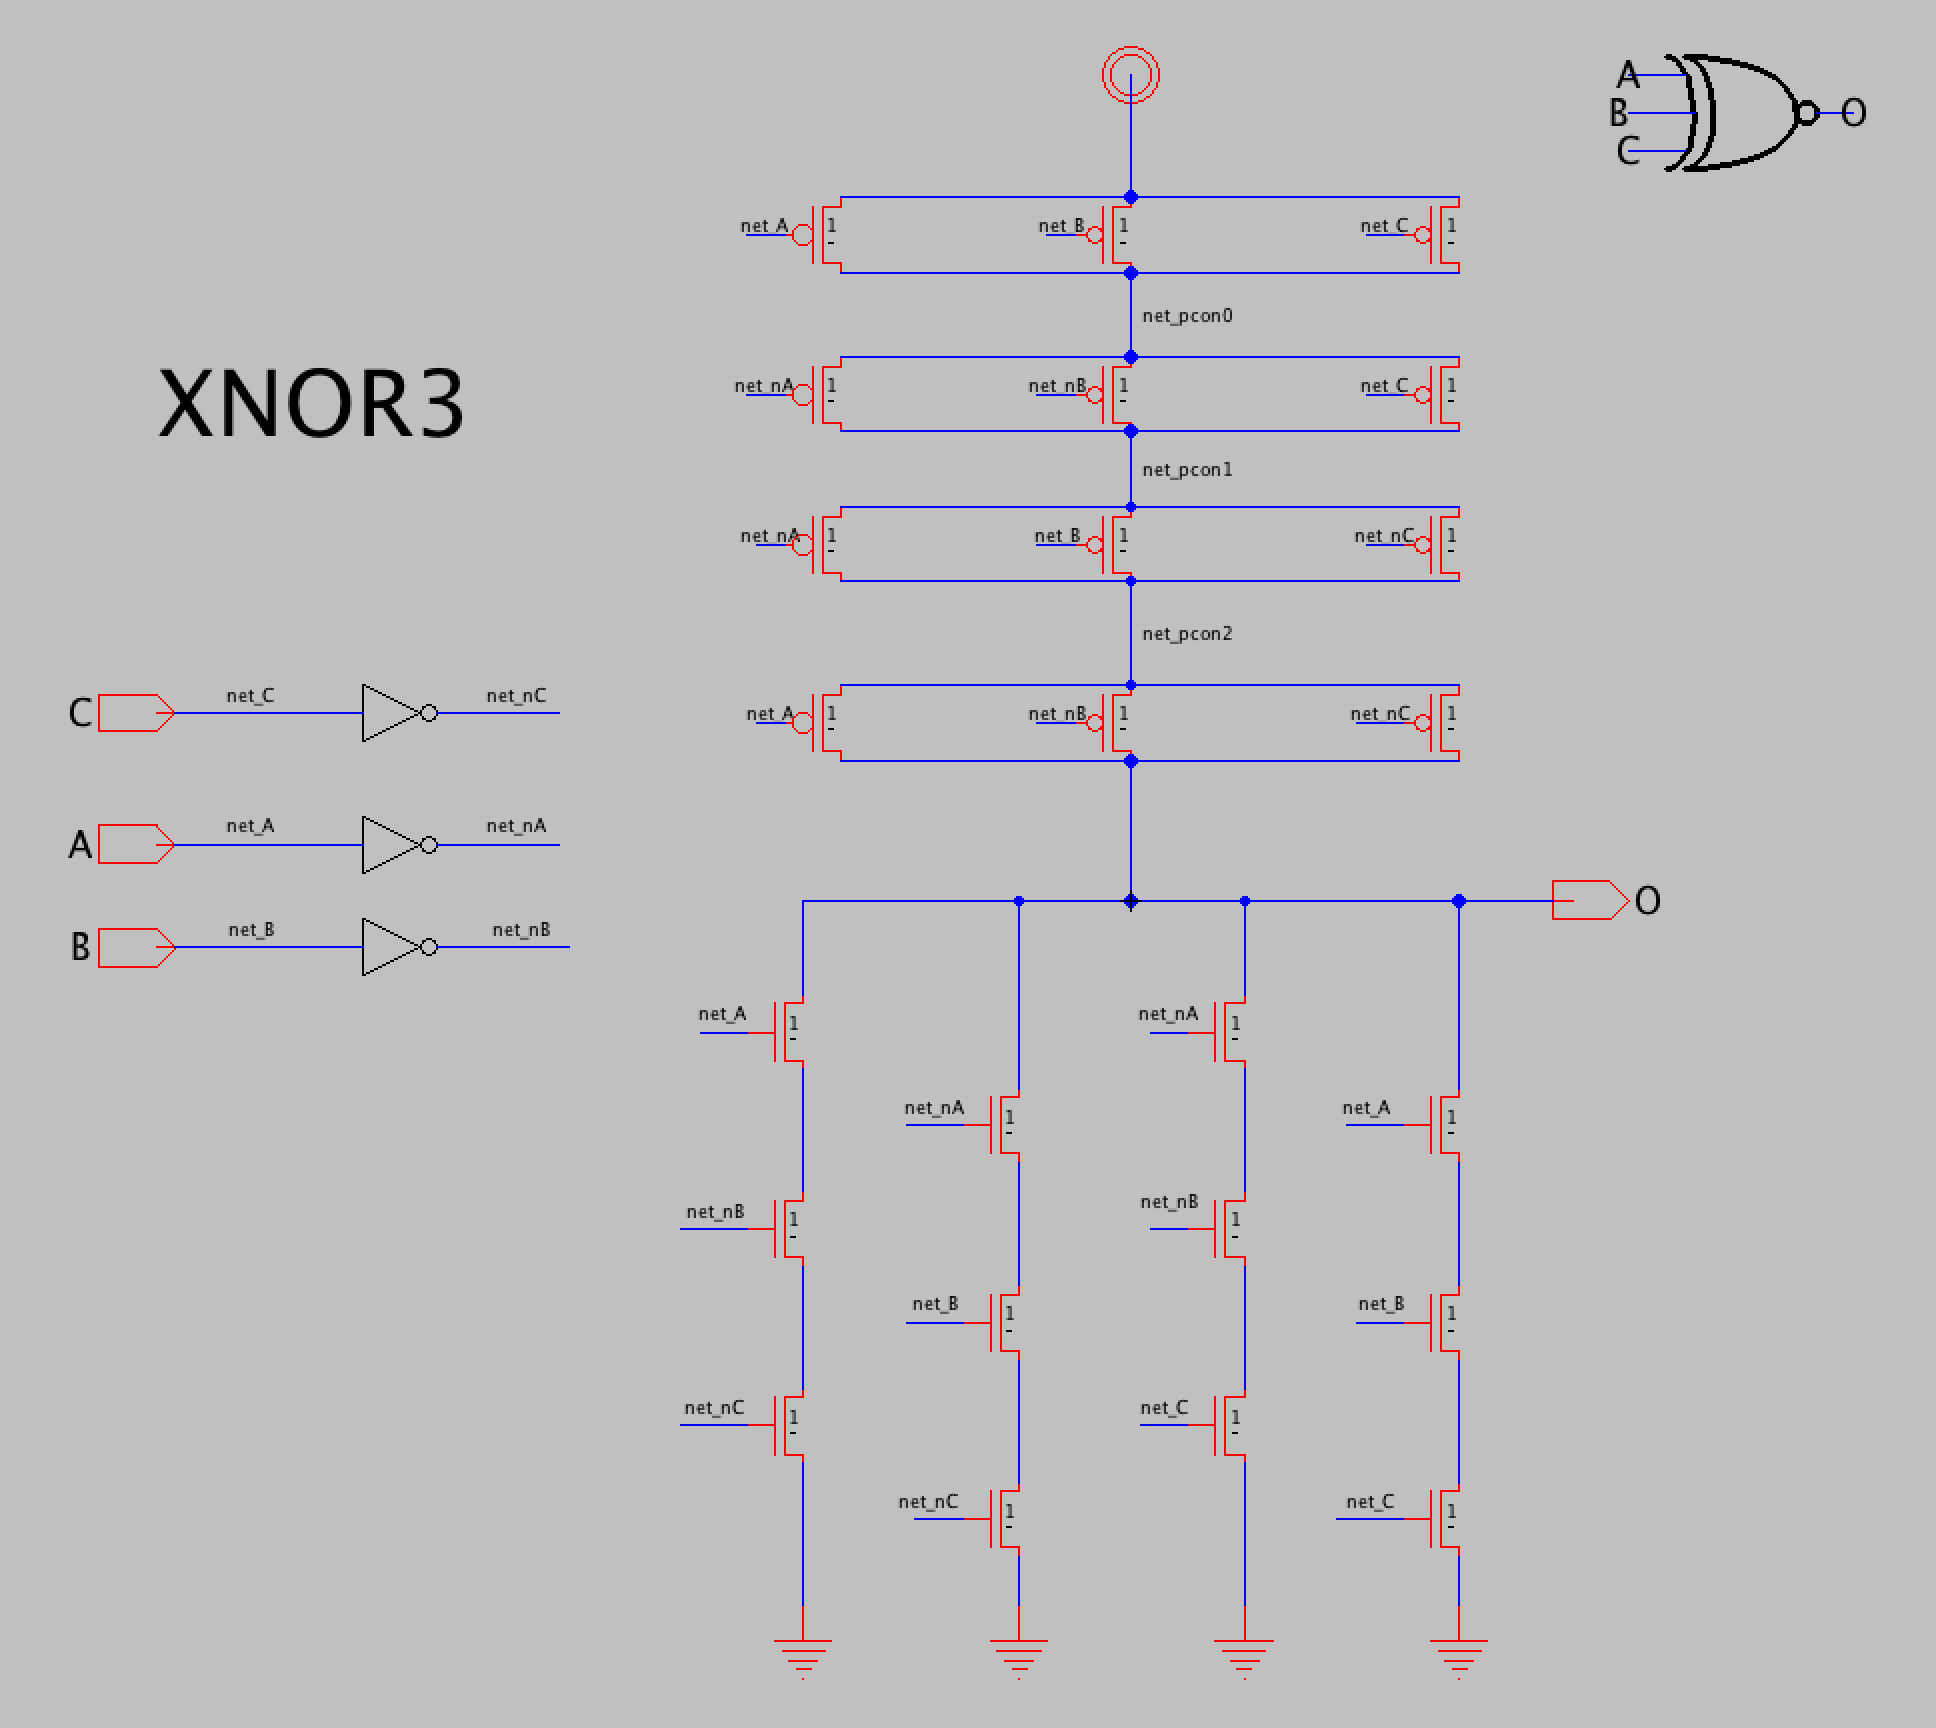
\includegraphics[width=\linewidth]{baseline_screenshots/XNOR3.png}
  \caption{3-input XNOR Gate}
  \label{fig:3inputnor}
\end{figure}

\begin{figure}[H]
  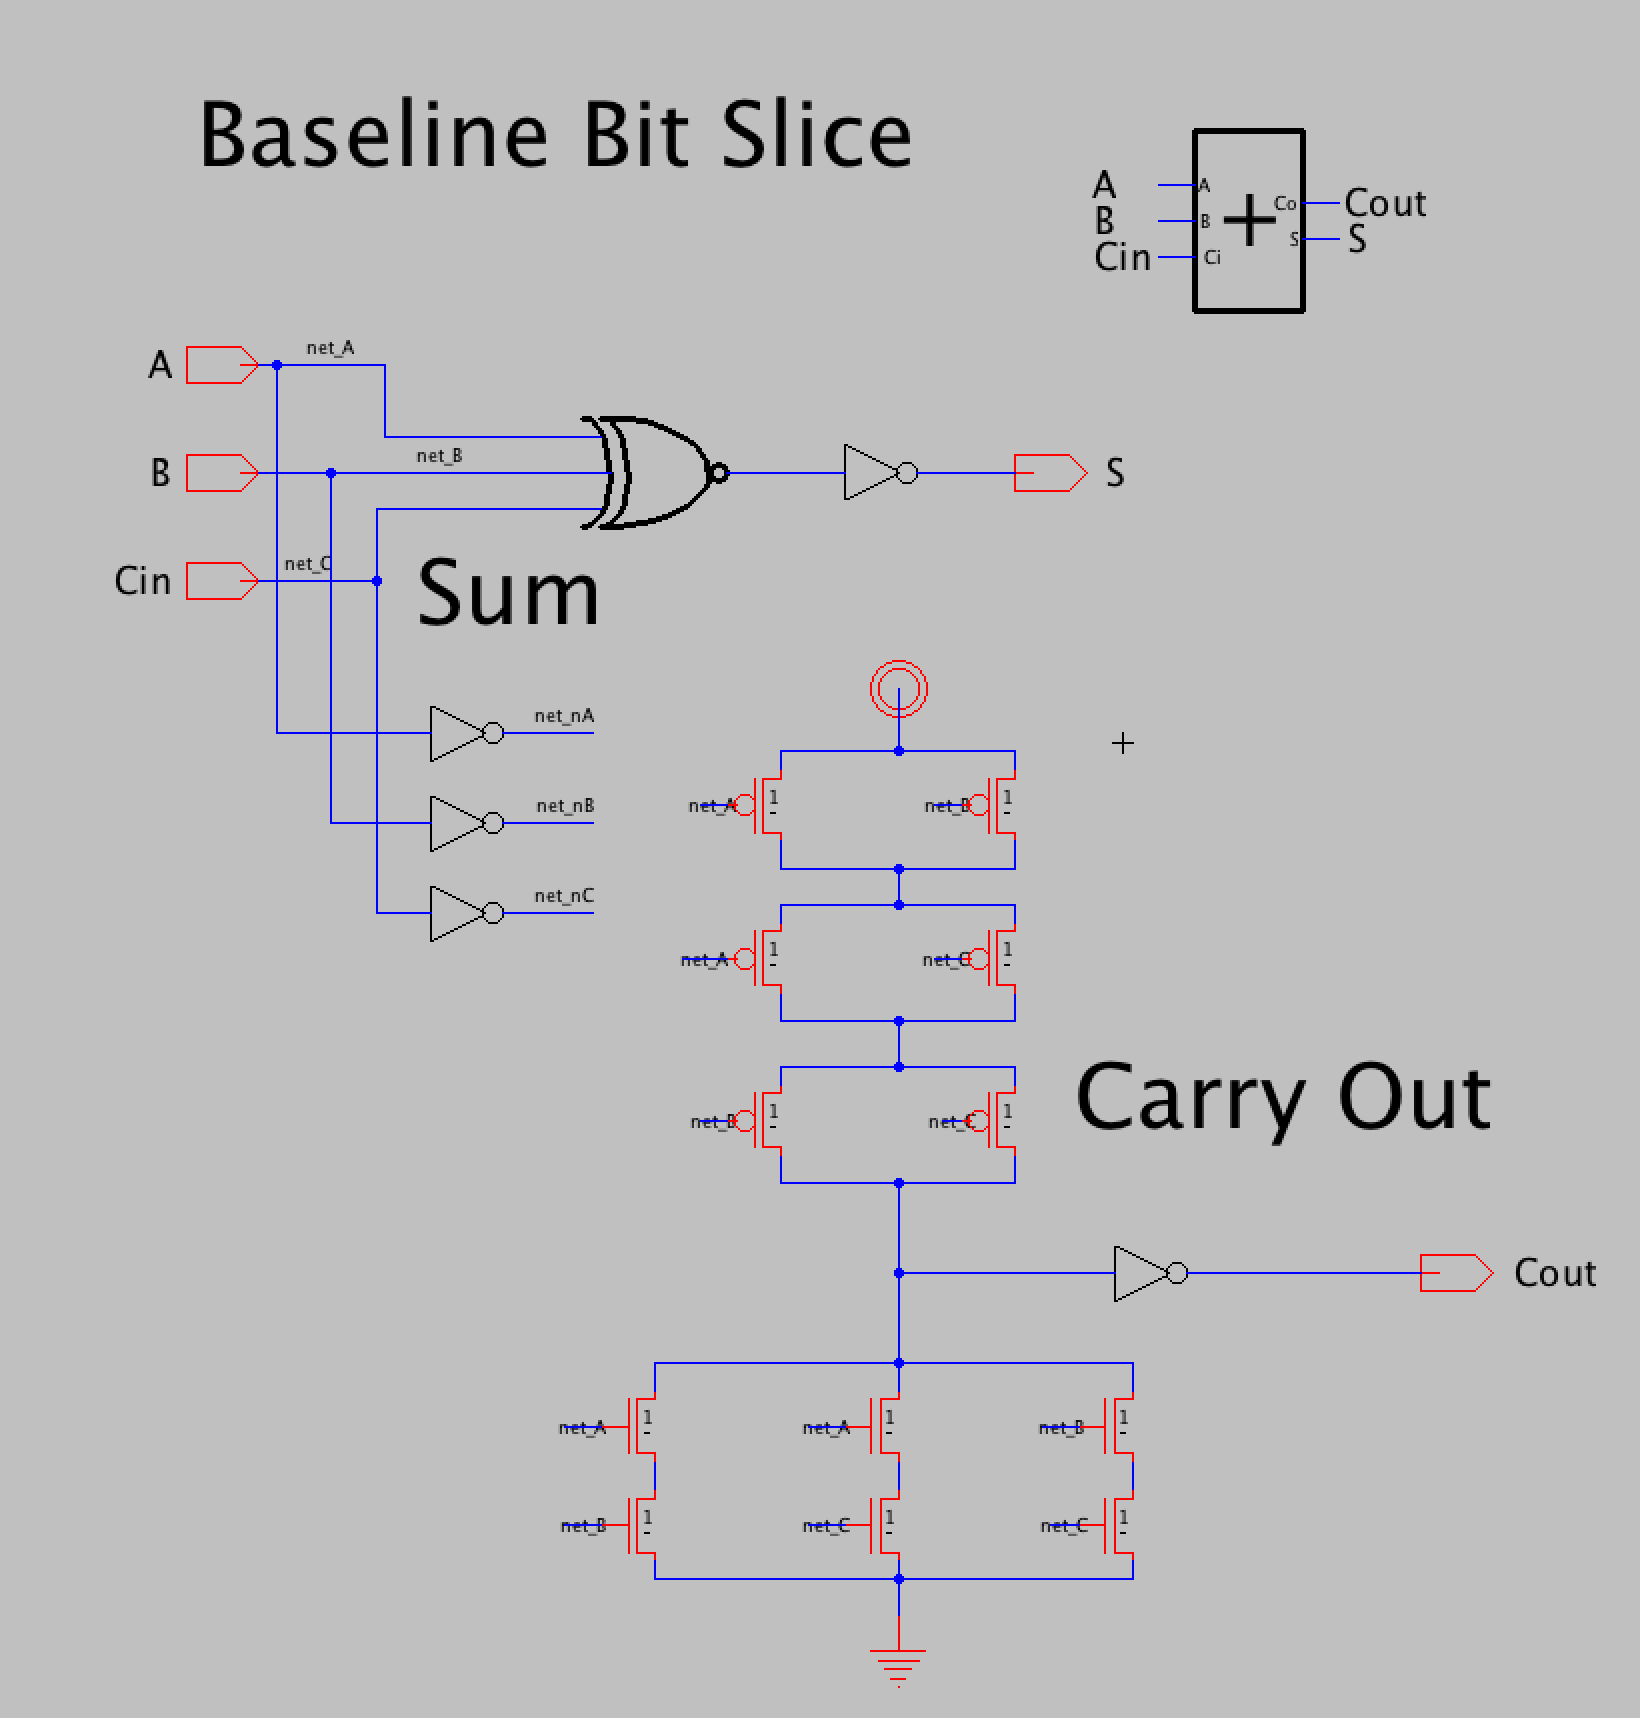
\includegraphics[width=\linewidth]{baseline_screenshots/baseline.png}
  \caption{Baseline Bit Slice Cell Schematic}
  \label{fig:baselinesch}
\end{figure}
\pagebreak

\section{Analysis of Baseline Design}

\subsection{Logical Correctness}
\subsubsection{Bit Slice}
First I validated the logical correctness of a single bit slice. The single bit slice should have the same input/output combinations as Figure \ref{fig:waveform1}. You can see the result in Figure \ref{fig:waveform_baseline_test_logic} and the setup in Figure \ref{fig:baseline_test_logic}. You'll notice that the output waveform is equivalent to the one in Figure \ref{fig:waveform1}.

\begin{figure}[H]
  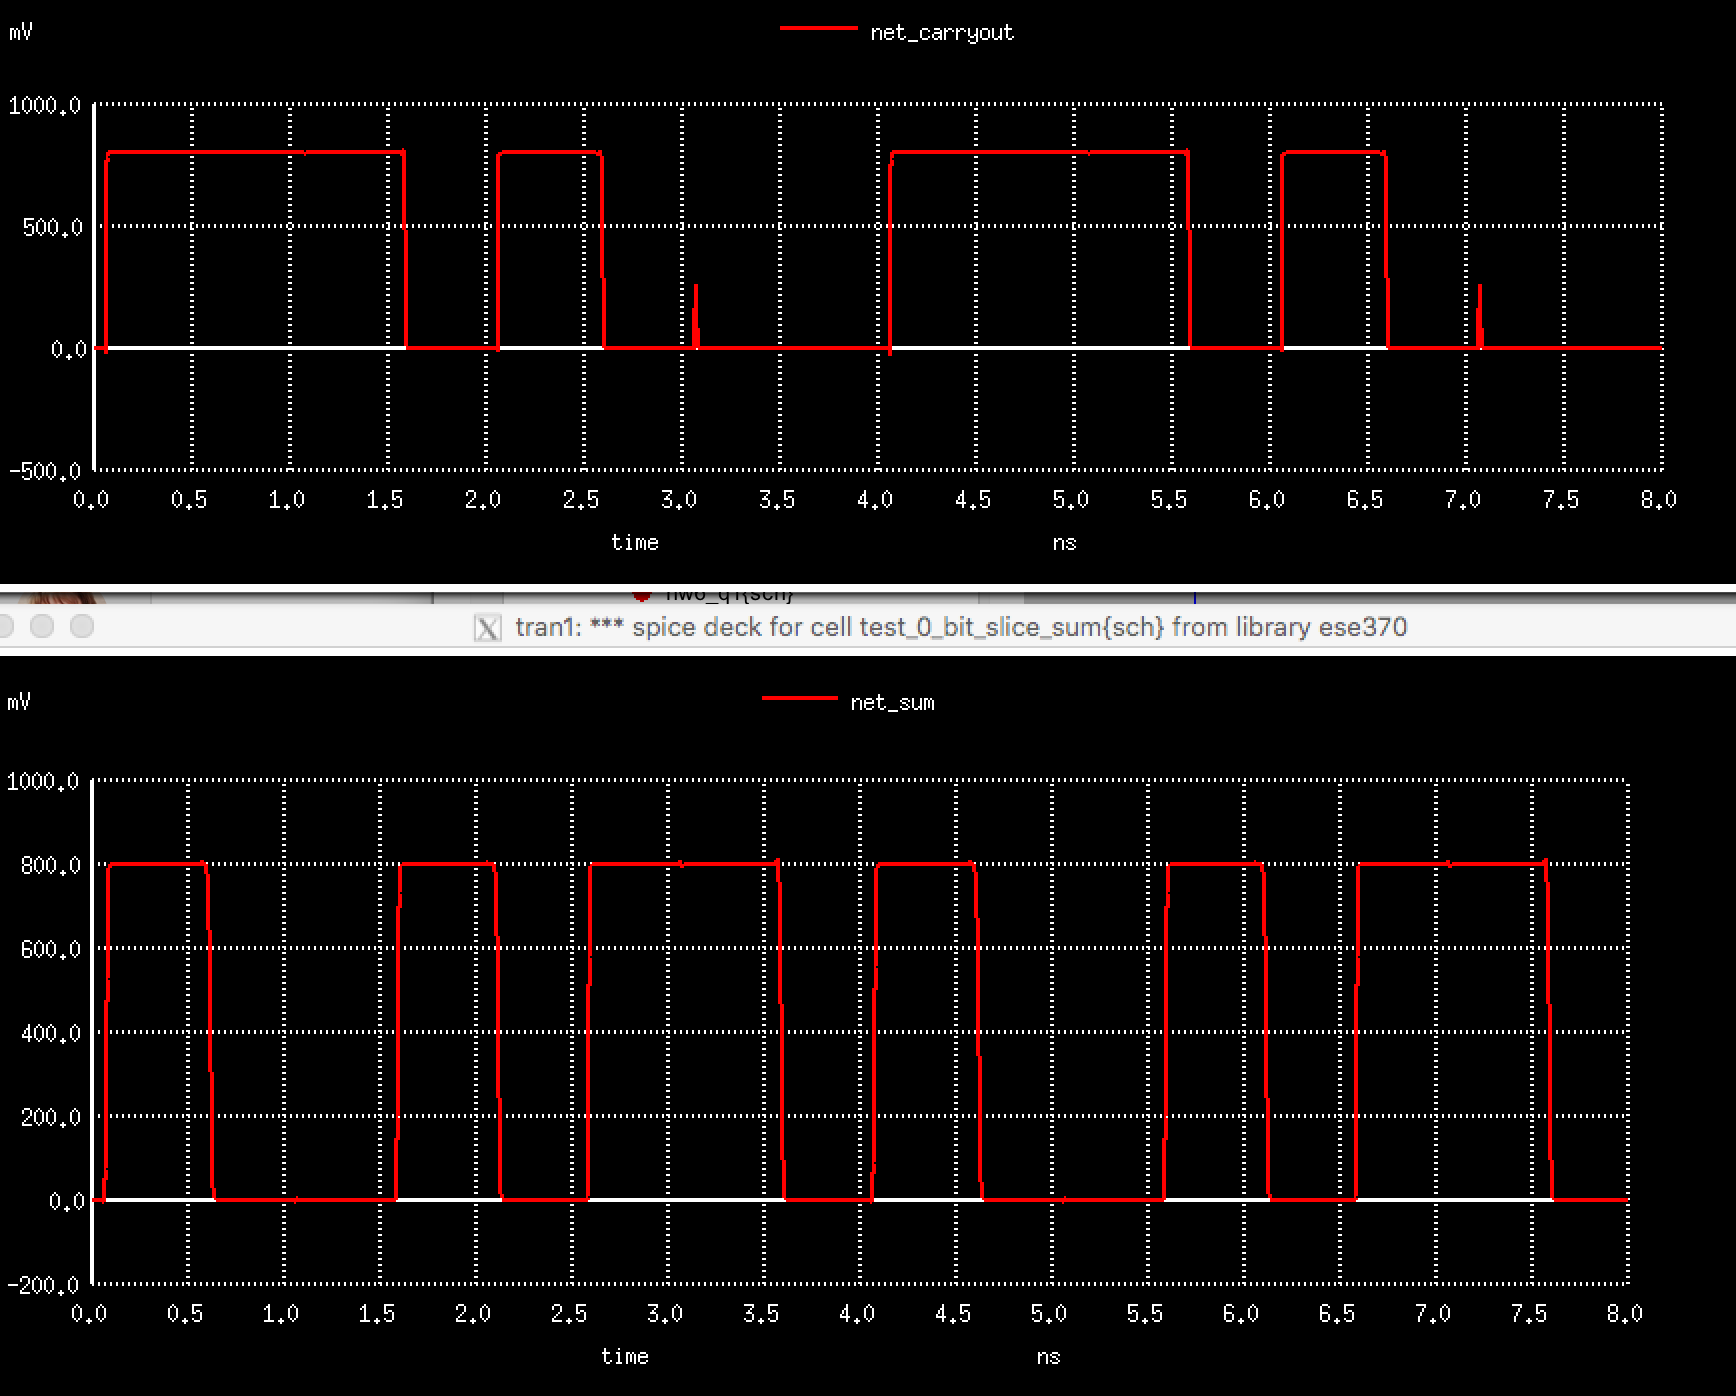
\includegraphics[width=\linewidth]{baseline_screenshots/baseline_test_logic_waveform.png}
  \caption{Output waveform for baseline logical test}
  \label{fig:waveform_baseline_test_logic}
\end{figure}

\begin{figure}[H]
  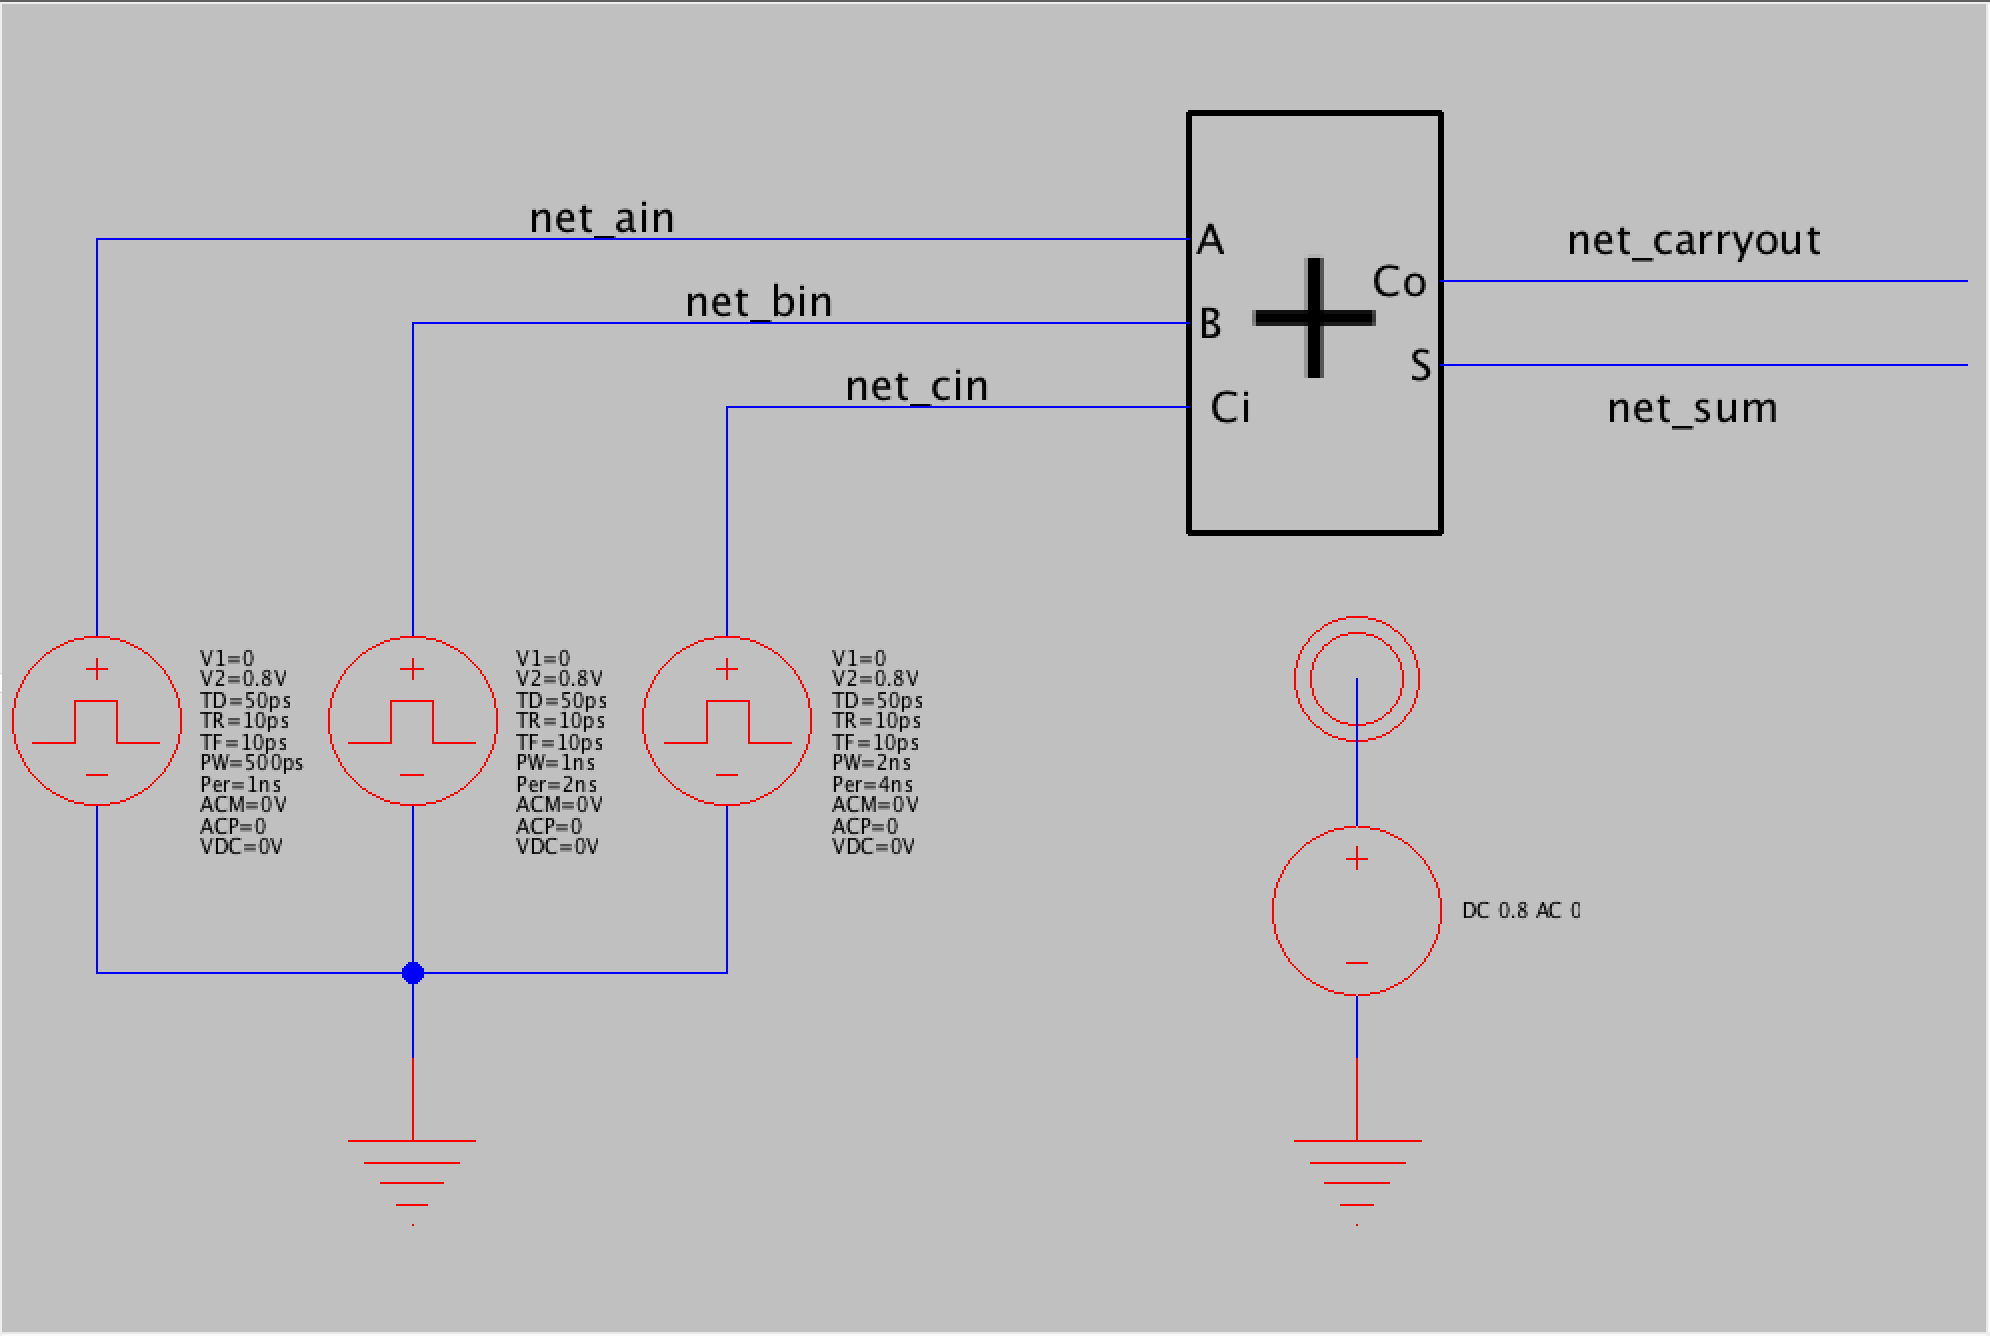
\includegraphics[width=\linewidth]{baseline_screenshots/baseline_test_logic_sch.png}
  \caption{Schematic for testing logical correctness of the baseline}
  \label{fig:baseline_test_logic}
\end{figure}

\subsubsection{Entire Adder}
I validated logical correctness for the entire adder in two ways. The first was by using the same input structure as in Figure \ref{fig:waveform1}. The second way was to check the 4 possible inputs for A and B. To do that, I used the inputs $(A, B) = (0xffff, 0xffff) \rightarrow (0x0000, 0xffff) \rightarrow (0xffff, 0x0000) \rightarrow (0x0000, 0x0000)$. This gives Figure \ref{fig:test_logic_16b_adder2}.

\begin{figure}[H]
  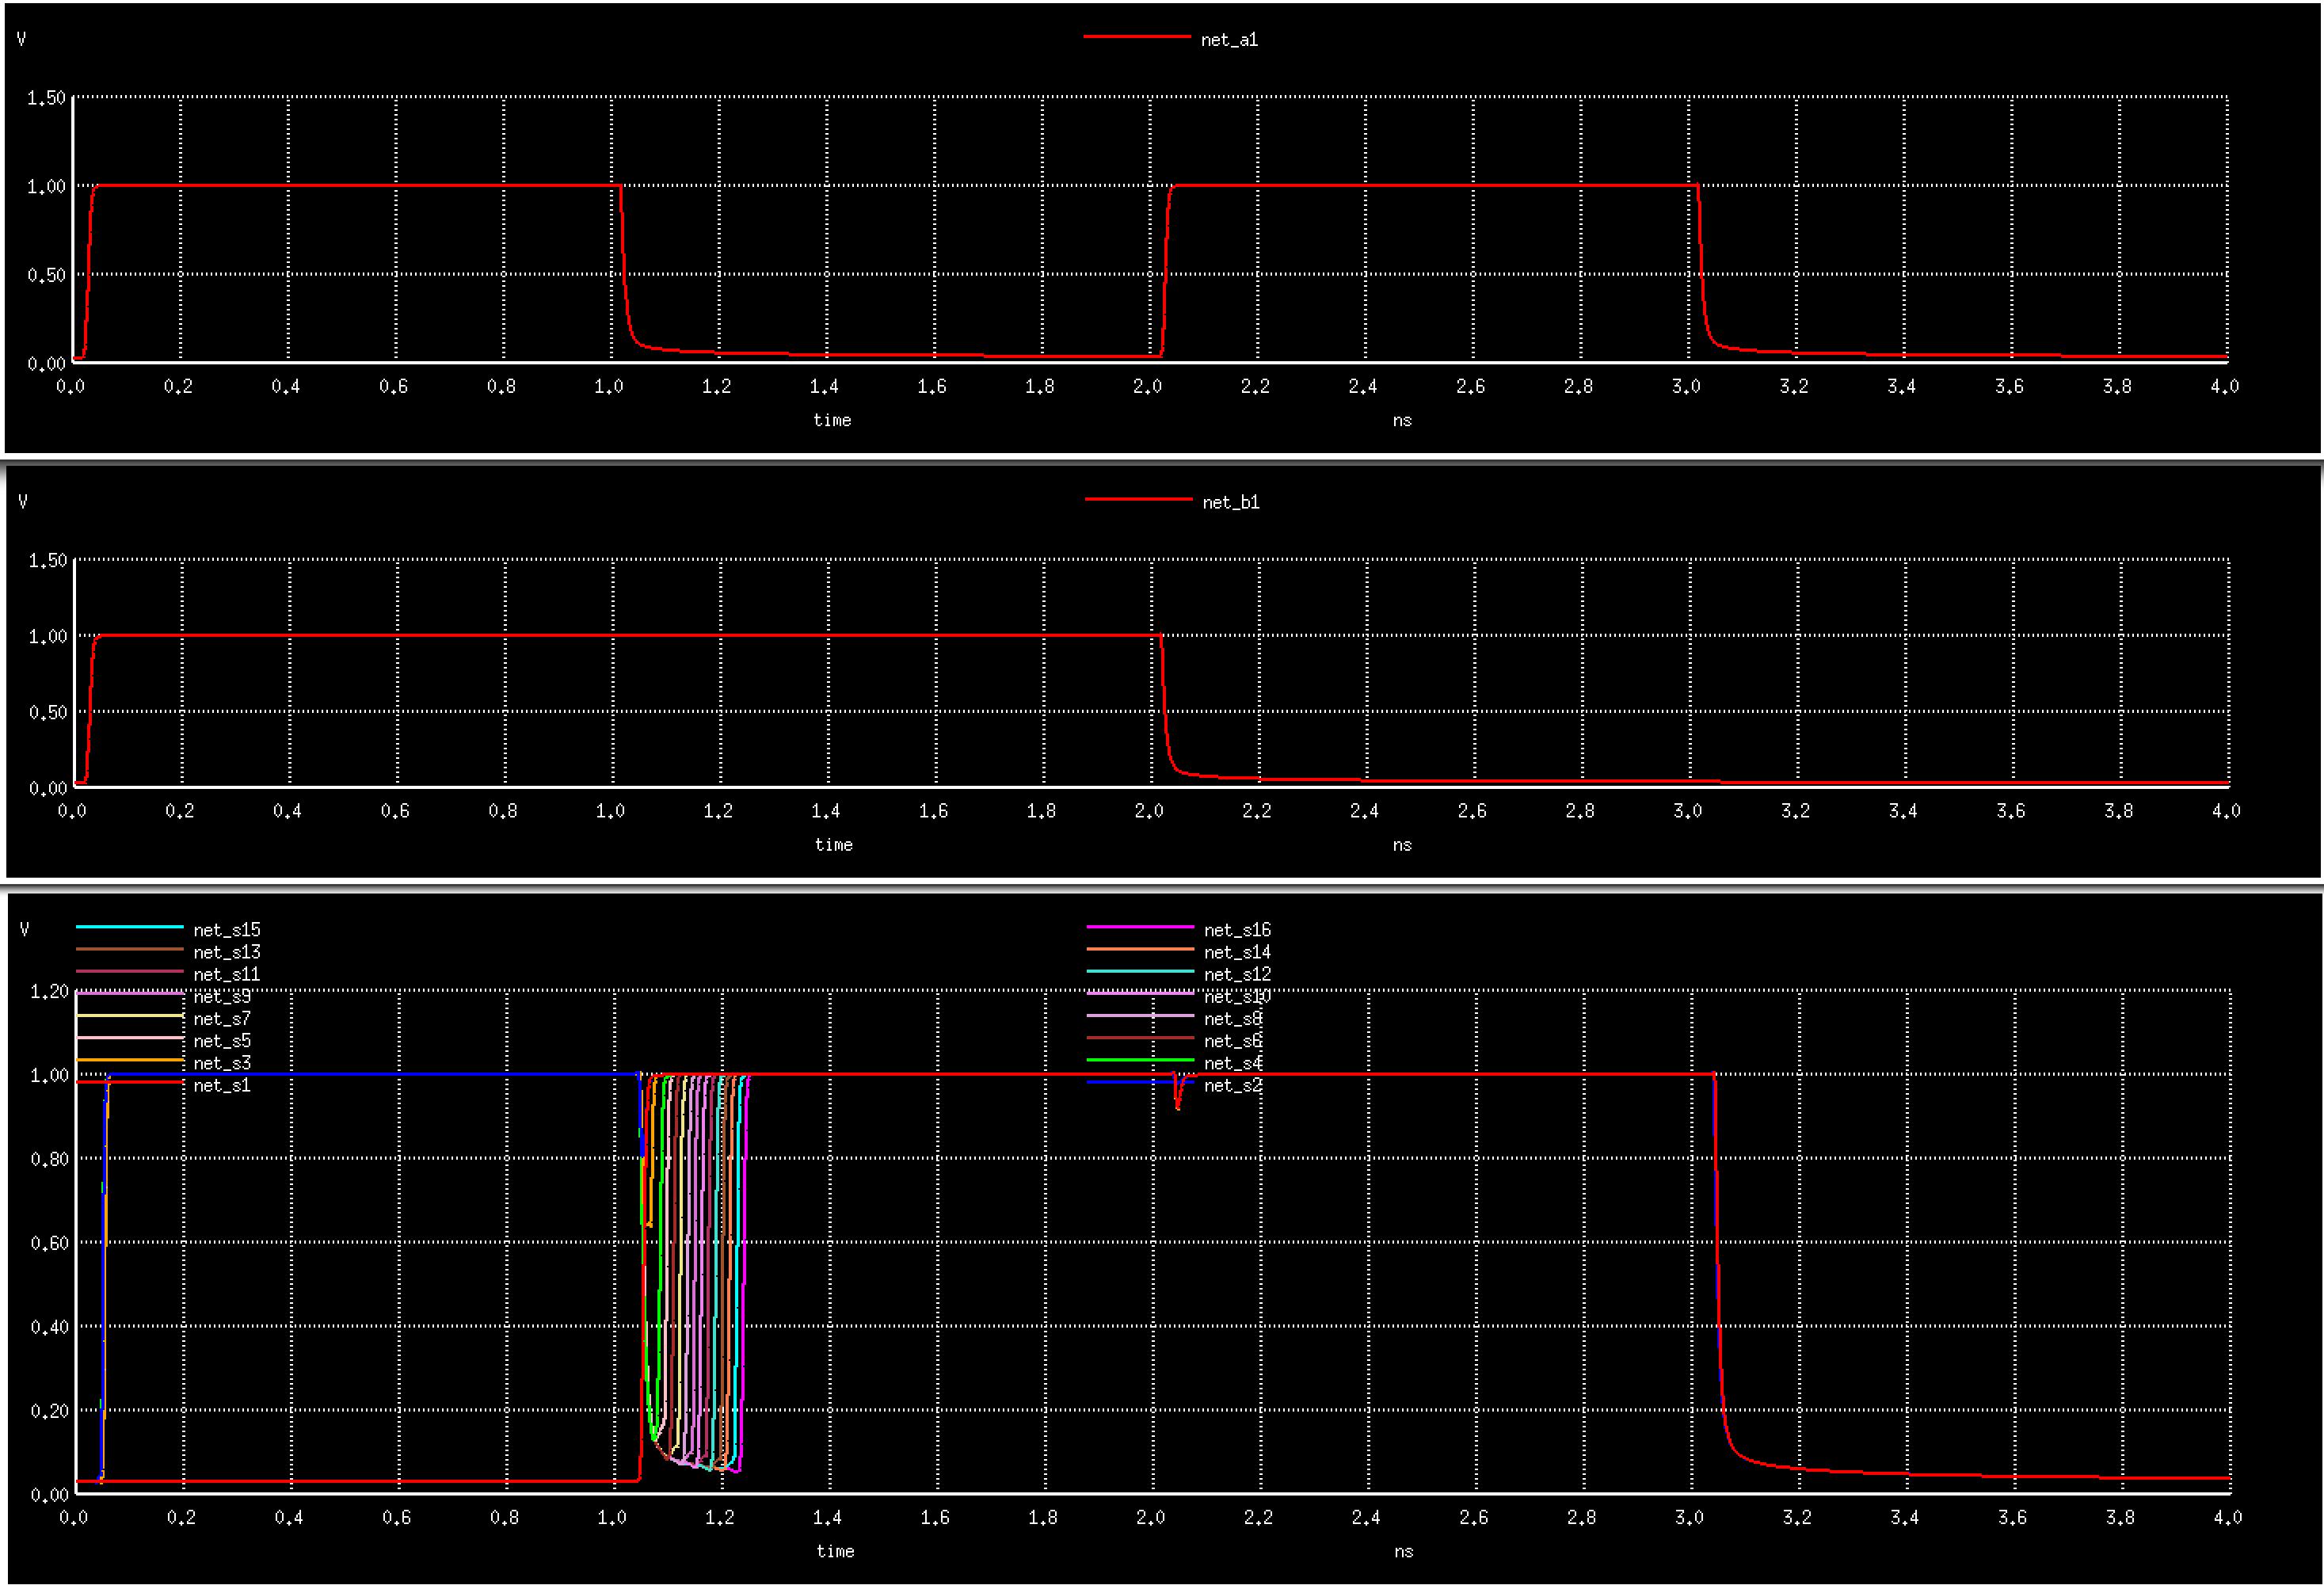
\includegraphics[width=\linewidth]{opt_screenshots/test_logic_16b_adder.png}
  \caption{Waveform showing logical correctness of the 1-bit nAdder}
  \label{fig:test_logic_16b_adder2}
\end{figure}

\subsection{Delay} 
The max delay of the baseline design is input $A = 0xffff, B = 0x0000 \rightarrow 0x0001$ is approximately $358\tau$, which is caused by the rippling carry to the final output and is calculated below.\\

\subsubsection{Calculating Sum Delay: Bit Slice}
For the delay of the sum, we calculate the delay from the input across the XNOR gate's internal inverter, and then across the XNOR gate and then across the final inverter to the output.
\begin{align*}
d_{s} &= d_{input \rightarrow inv1} + d_{inv1 \rightarrow xnor} + d_{xnor \rightarrow inv2} + d_{inv2 \rightarrow output}\\
d_{input \rightarrow inv1} &= R_{output}C_{input}\\
C_{input} &= C_A = C_B = C_{Cin}\\
C_A &= C_{xnor_{in}} + C_{Cout_{in}}\\
&= 4C_0 + 4C_0\\
&= 8C_0\\
R_{drive} &= R_0\textnormal{ because of the single inverter on the output}\\
d_{input \rightarrow inv1} &= R_{output}C_{input}\\
&= (1R_0)(10C_0)\\
&= 10\tau\\
d_{inv \rightarrow xnor} &=  R_{inv}C_{xor_{in}}\\
&= (1R_0)(4C_0)\\
&= 4\tau\\
d_{xnor \rightarrow inv2} &= R_{xor}C_{inv2}\\
&= (4R_0)(2C_0)\\
&= 8 \tau\\
d_{inv2 \rightarrow output} &= R_{inv2}C_{input}\\
&= (1R_0)(8C_0)\\
&= 8\tau\\
d_{s} &= d_{input \rightarrow inv1} + d_{inv1 \rightarrow xnor} + d_{xnor \rightarrow inv2} + d_{inv2 \rightarrow output}\\
&= 8\tau + 4\tau + 8\tau + 8\tau\\
&= 28\tau
\end{align*}

\subsubsection{Calculating Carry Out Delay: Bit Slice}
Calculating the delay of the carry out is straightforward. First, we consider the input delay, which is the same as above. Next, we consider the gate and inverter, and finally the output and its load.
\begin{align*}
d_{Co} &= d_{input \rightarrow gate} + d_{gate \rightarrow inv_{output}} + d_{inv_{output} \rightarrow output}\\
d_{input \rightarrow gate} &= 8\tau\\
d_{gate \rightarrow inv_{output}} &= R_{gate}C_{inv}\\
&= (3R_0)(2C_0)\\
&= 6\tau\\
d_{inv_{output} \rightarrow output} &= R_{inv}C_{load}\\
&= (1R_0)(8C_0)\\
&=8\tau\\
d_{s} &= d_{input \rightarrow gate} + d_{gate \rightarrow inv_{output}} + d_{inv_{output} \rightarrow output}\\
&= 8\tau + 6\tau + 8\tau\\
&=22\tau\\
\end{align*}
\\

\subsubsection{Measured Delay: Bit Slice}
I graphed the delay and measured from $0.4V$ on the input to $0.4V$ on the output as we have done in previous assignments. The setup is shown in Figure \ref{fig:baseline_16b_adder_sch_zoomed}. The delay for a single bit slice is measured in the switching case $(A, B, Cin) = (0 \rightarrow 1, 0, 0)$ since this only allows one path through the pull up network, and thus avoids a reduction in $R_{on}$ by parallel PMOS transistors. These inputs need to be driven by an equivalent drive of the sum gate, so I created a driver as shown in Figure \ref{fig:baseline_sum_driver_sch} to drive the inputs to all bit slices and load all sum outputs.\\
The total delay across the sum is: $63.7879ps$(Figure \ref{fig:sum_out_waveform})\\
The total delay across the carry is: $37.3973ps$(Figure \ref{fig:carry_out_waveform})\\
\textbf{Calculations}\\

\textit{For $\tau$:}\\
\begin{align*}
R_{on} &= 21454.6\Omega\\
Co &= 0.1694fF\\
2.2 \tau &= 2.2 R_{on} \times Co\\
&= 2.2 \times 21454.6\Omega \times 0.1694fF \\
&= 7.9957003\times 10^{-12}s\\
&= 7.9957003ps\\
\end{align*}

\textit{For sum delay:}\\
\begin{align*}
28\tau &= 28 \times 7.9957003ps\\
&= 28 \times 7.9957003ps
&= 223.87961ps
\end{align*}

\textit{For carry out delay:}\\
\begin{align*}
22\tau &= 22 \times 7.9957003ps\\
&= 22 \times 7.9957003ps
&= 175.90541ps
\end{align*}

These values are much higher than the observed values most likely because of inaccuracies in $R_{on}$ and $Co$ observed in previous work. 

\begin{figure}[H]
  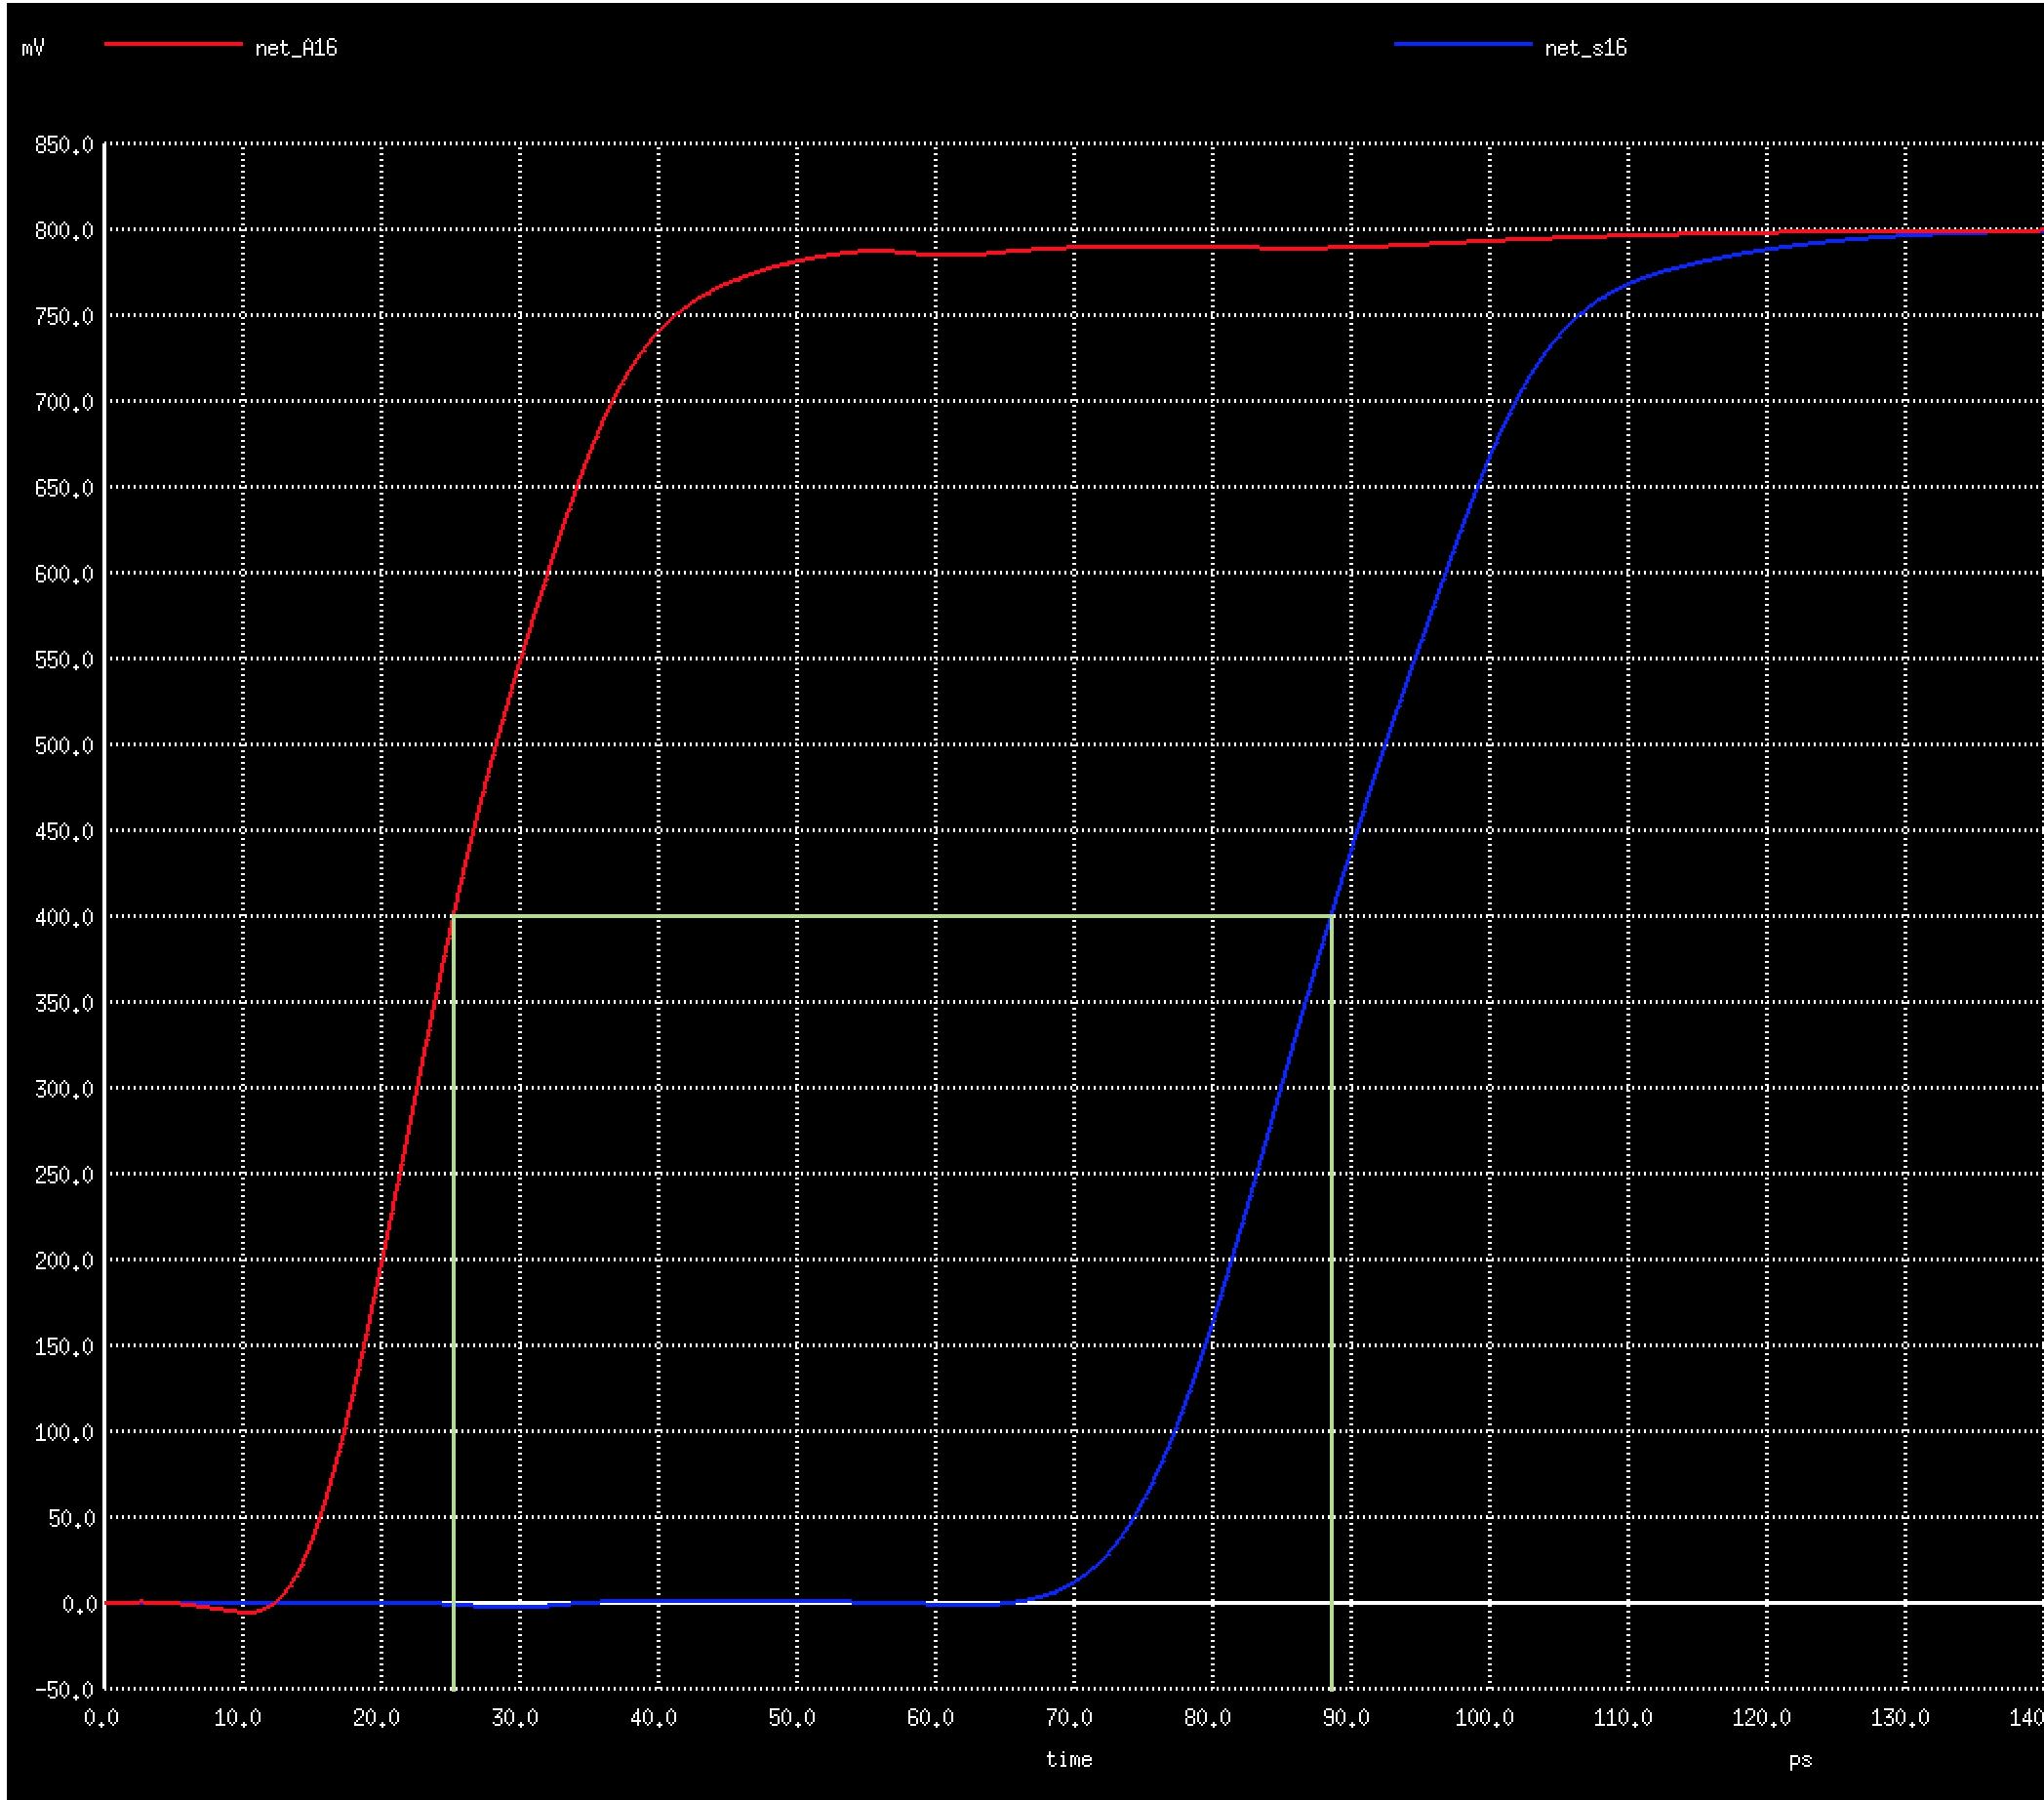
\includegraphics[width=\linewidth]{baseline_screenshots/sum_out_waveform.png}
  \caption{Waveform measuring input to output of baseline sum bit slice}
  \label{fig:sum_out_waveform}
\end{figure}

\begin{figure}[H]
  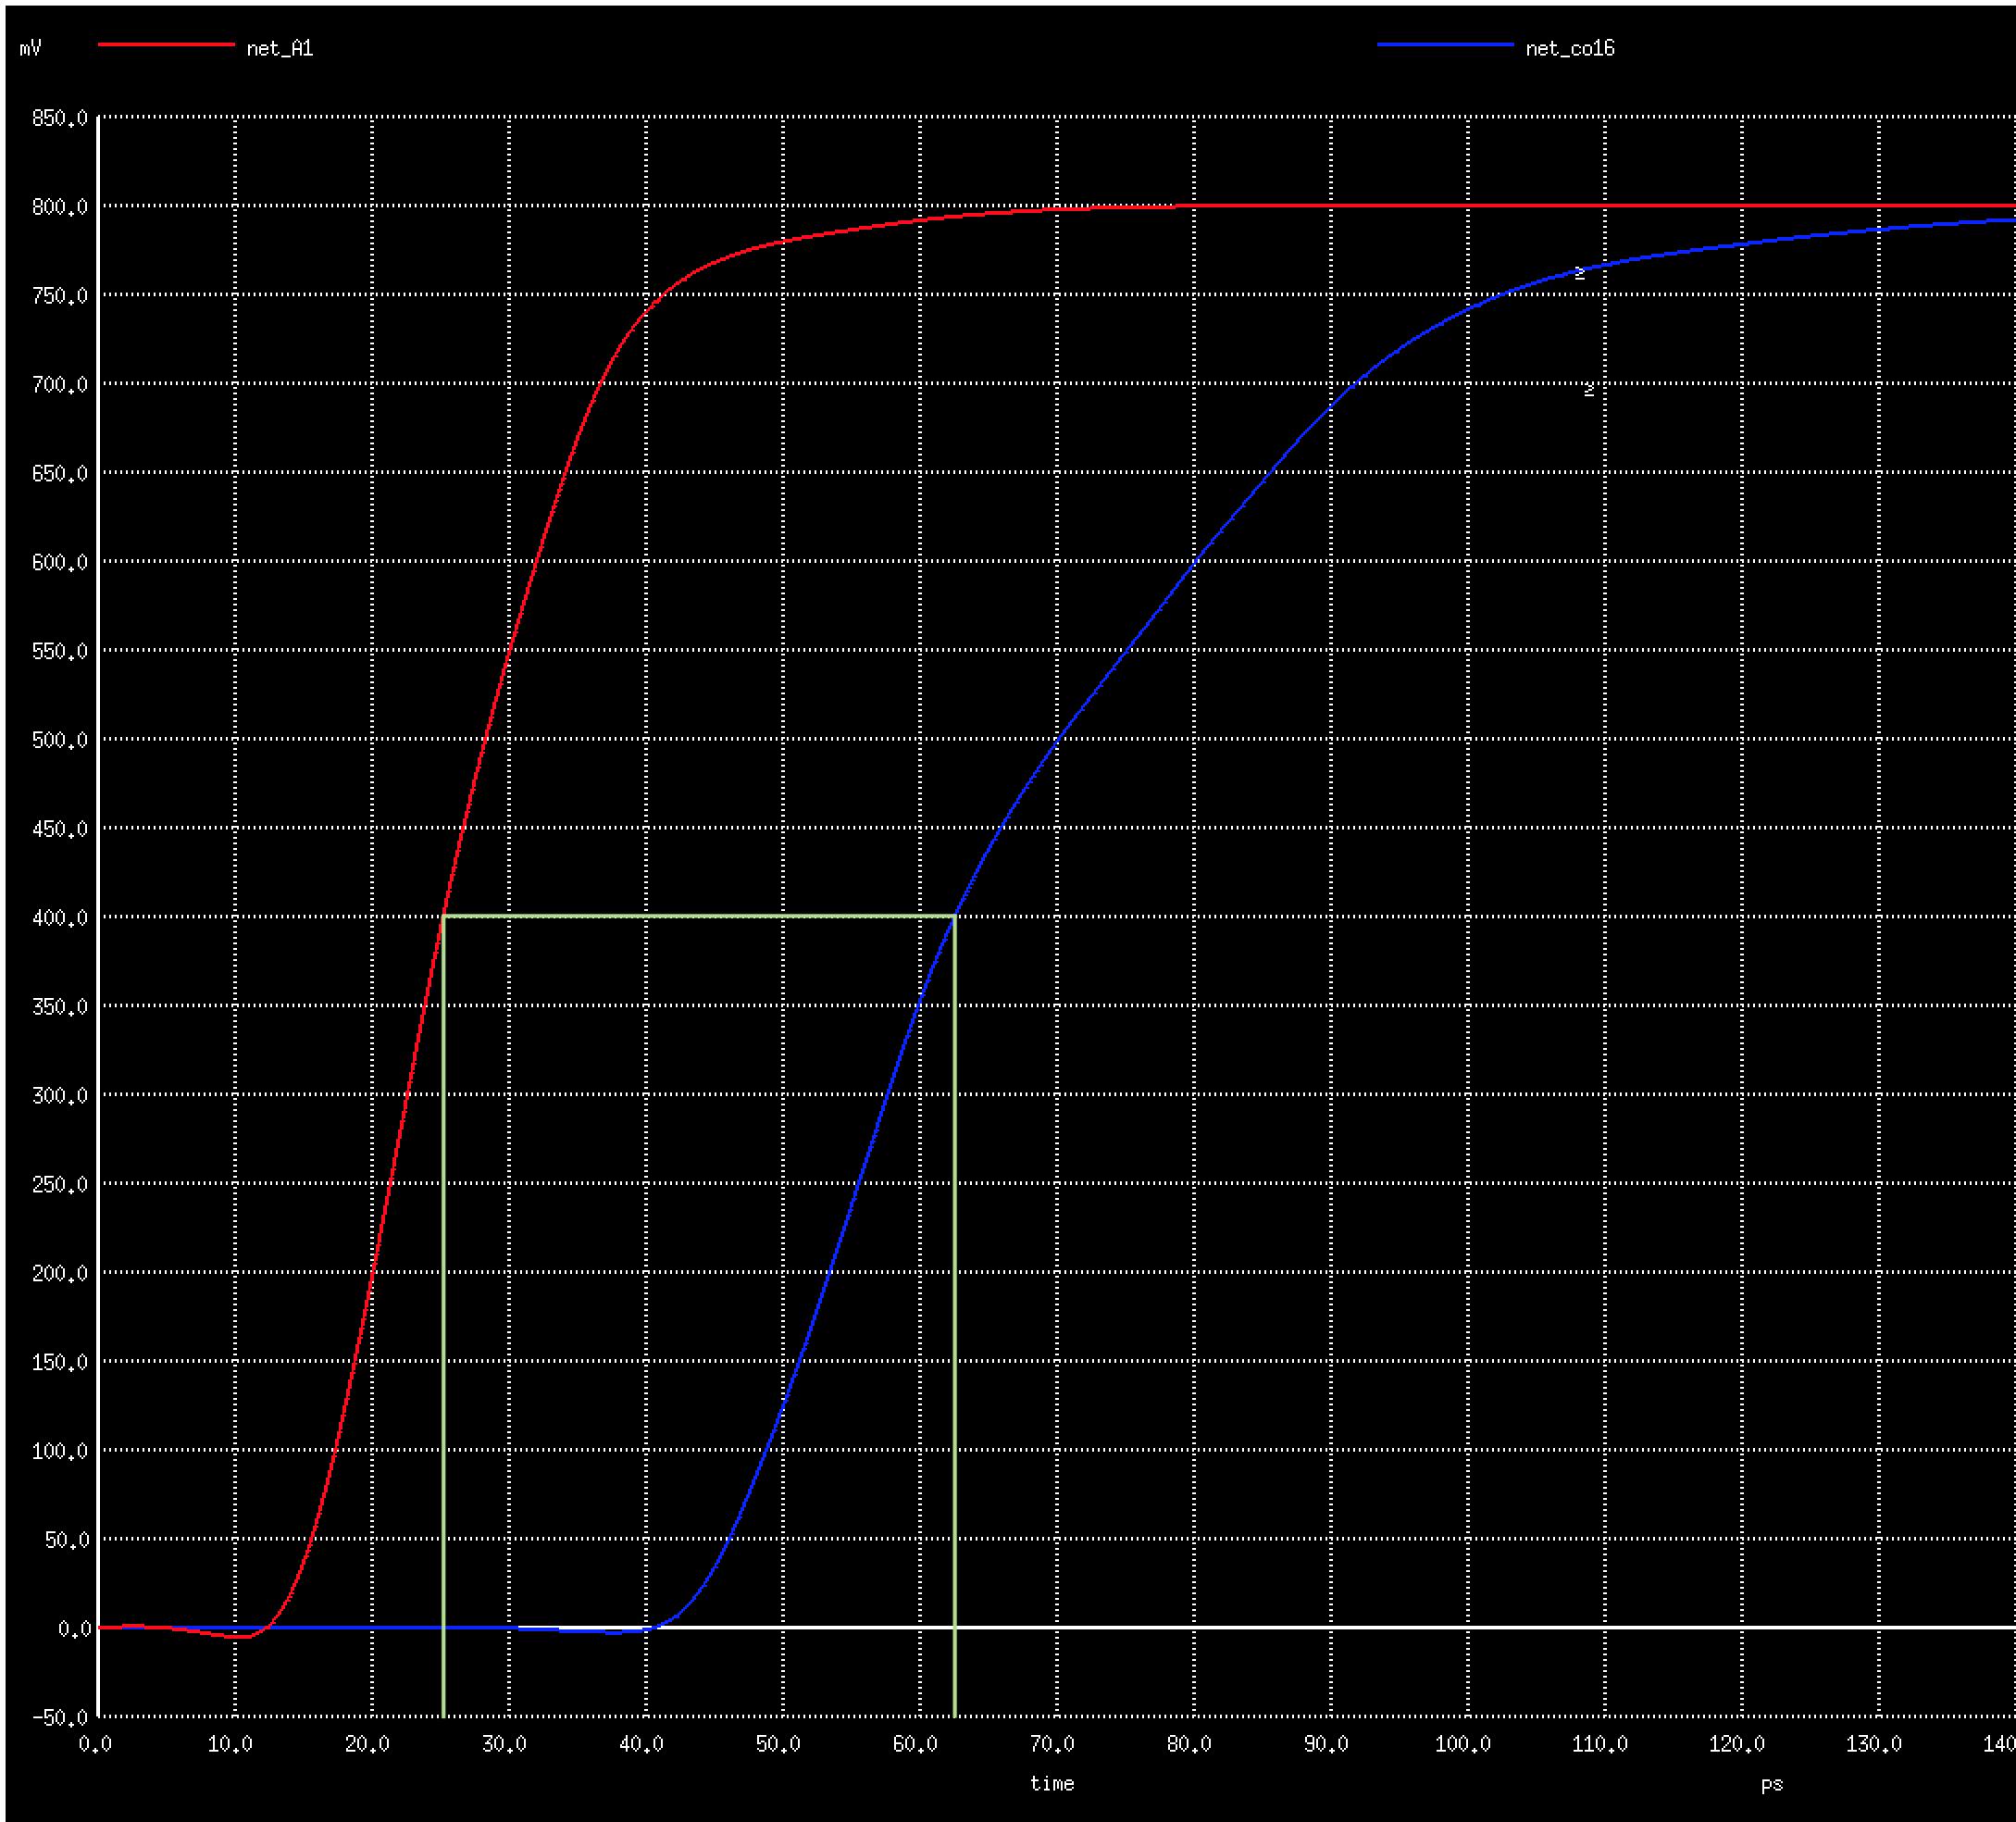
\includegraphics[width=\linewidth]{baseline_screenshots/carry_out_waveform.png}
  \caption{Waveform measuring input to output of carry out across a bit slice}
  \label{fig:carry_out_waveform}
\end{figure}

\subsubsection{Calculating Worst Case Delay: 16 Bit Adder}
The worst case delay occurs when the carry is propagated through the entire adder changing every sum output value, and the sum outputs rise. That is, in the case $(A, B, Sum) = (0xffff, 0x0001 \rightarrow 0x0000, 0x0000 \rightarrow 0xffff)$. Intuition led me to believe that the last value to rise should be the carry out. However, because of the large fan-in of the baseline sum gate, the sum output must drive a large capacitance, slowing the rise time as seen above in the calculated sum $\tau$ value. Therefore, the worst case delay is the time it takes for the carry out to propagate through 15 bit slices plus the time it takes for sum $16$ to rise.

\textit{For worst-case delay:}\\
\begin{align*}
d &= 15 \times d_{carry} + d_{sum}\\
&= 15 \times 22\tau + 28\tau\\
&= 358\tau
\end{align*}

\subsubsection{Measuring Worst Case Delay: 16 Bit Adder}
The worst-case delay was measured on the waveform in Figure \ref{fig:baseline_worst_case_delay} from $0.4V$ to $0.4V$, and the resulting worst case delay is $667.123ps$. Comparing this to the calculated $358 \times 7.9957003ps = 2.8624607ns$ shows the disparity caused my a wrong $C_0$ and $R_{on}$.

\begin{figure}[H]
  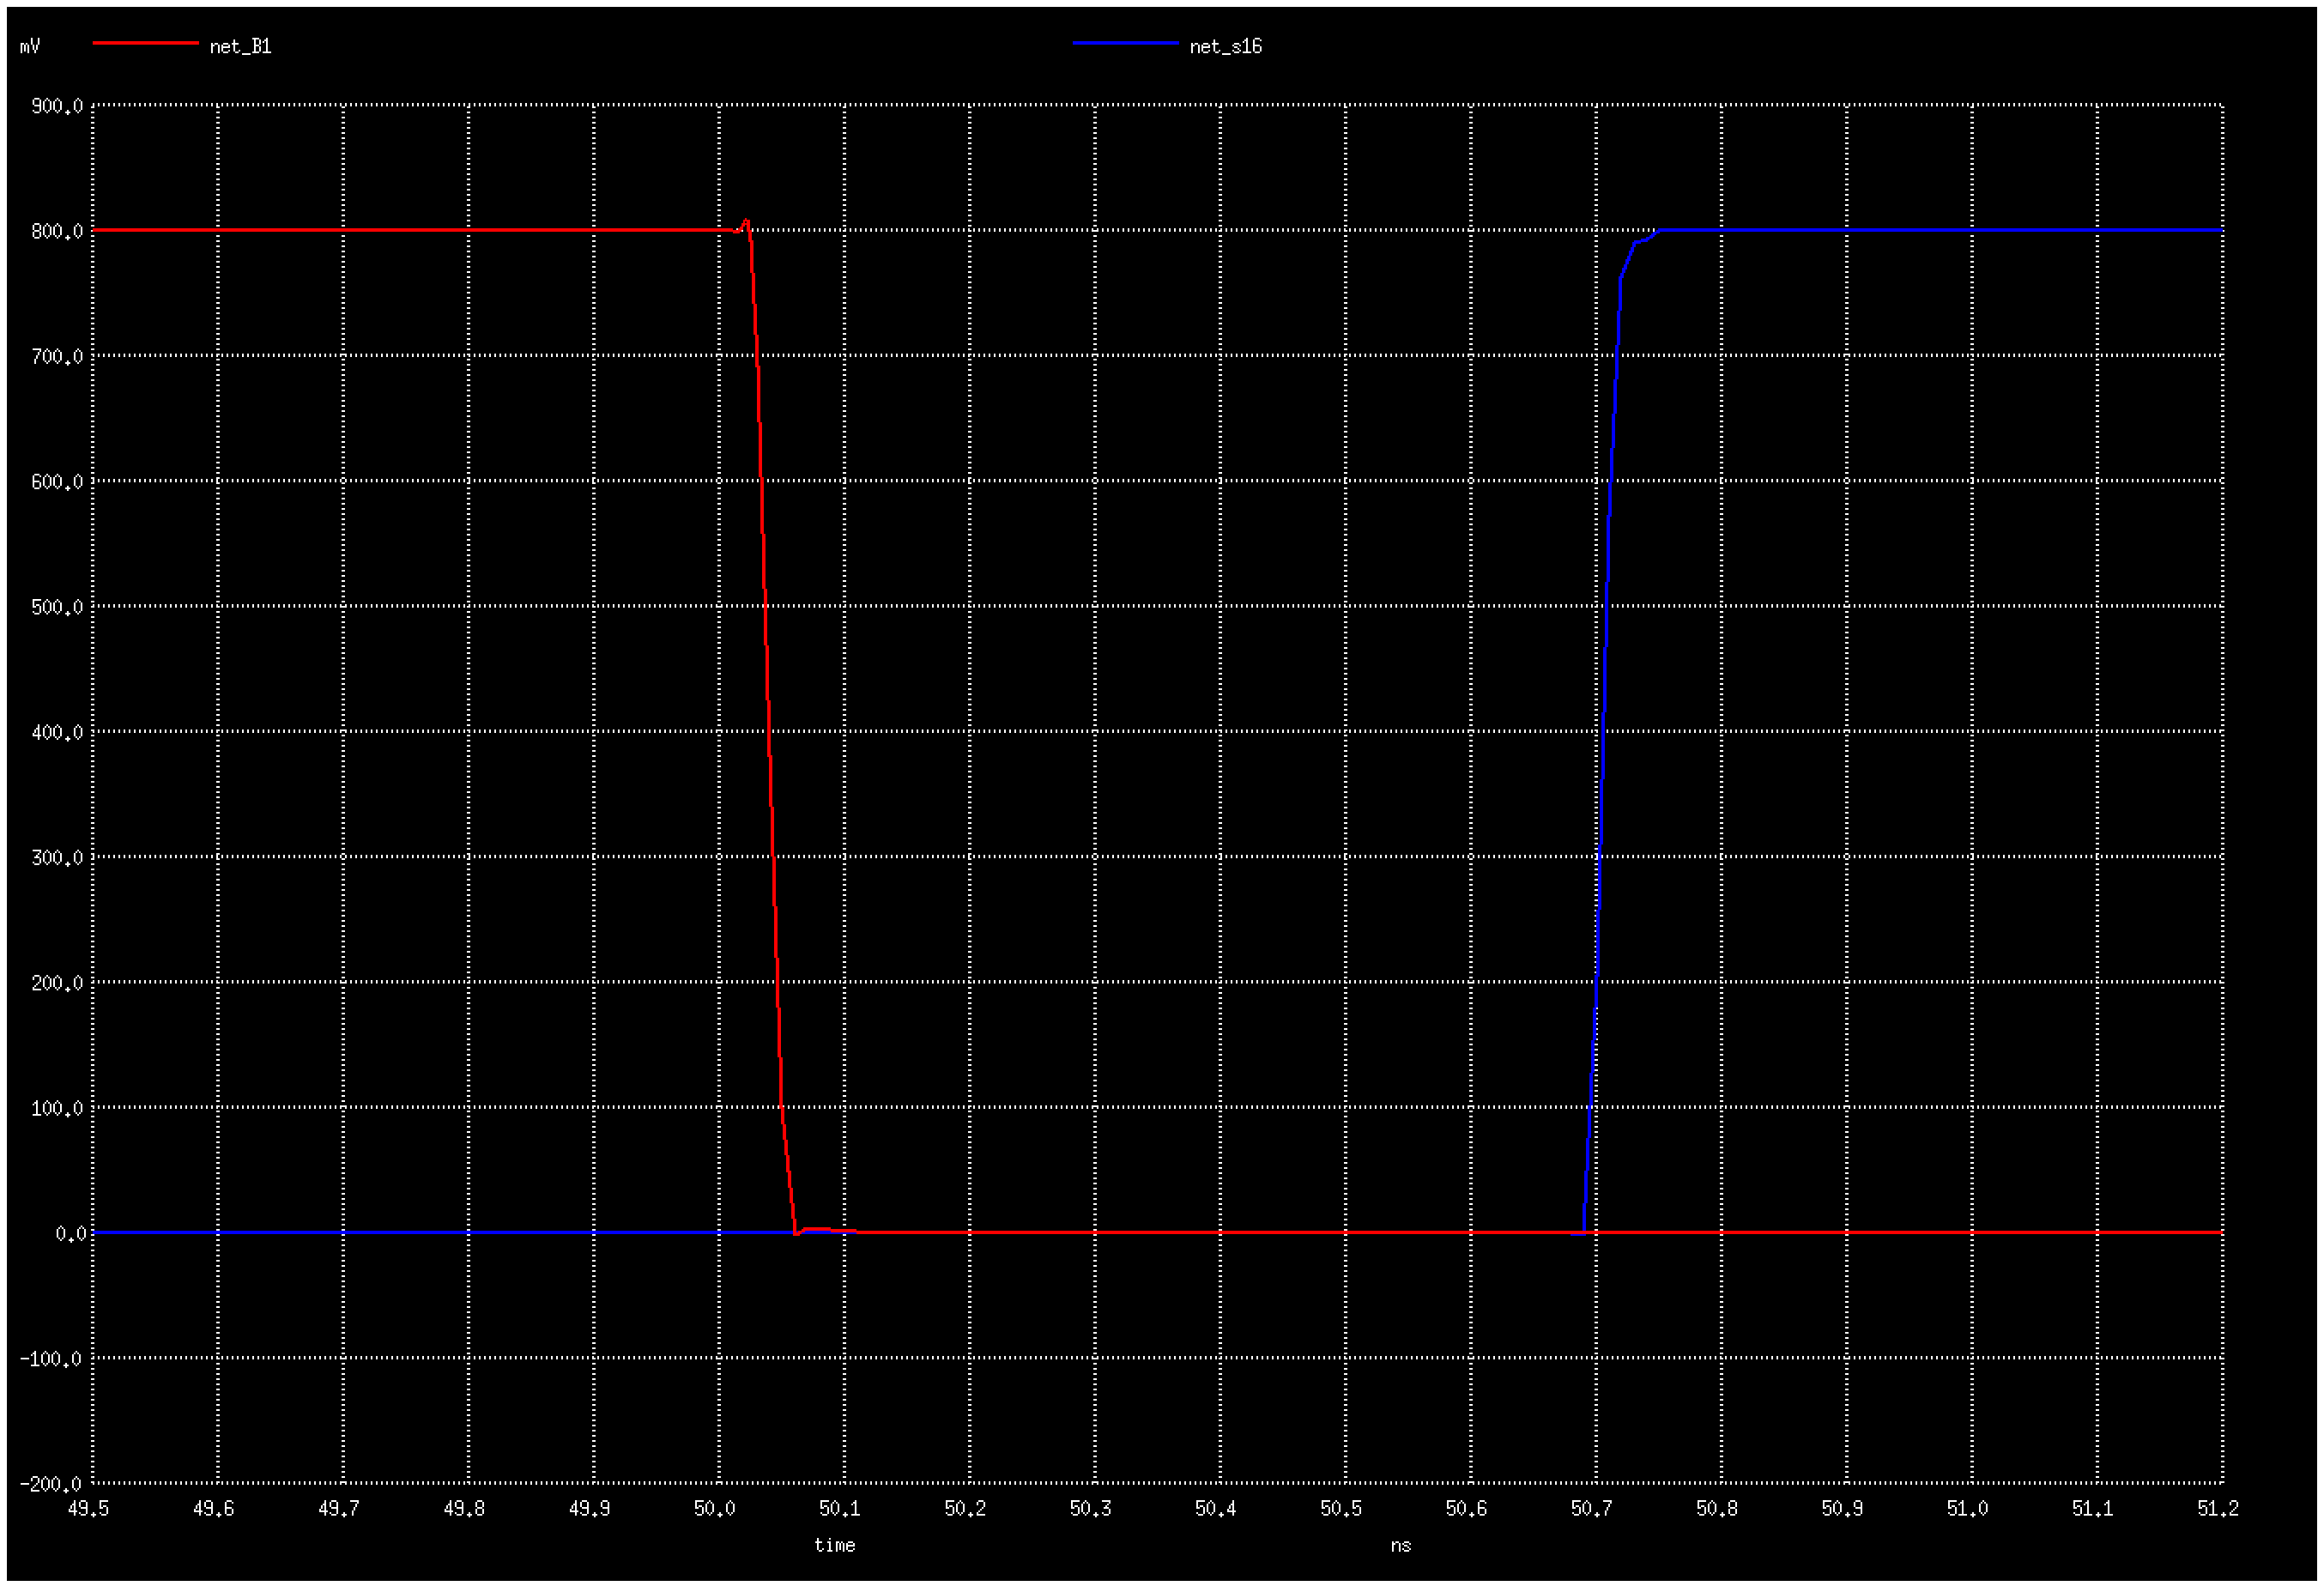
\includegraphics[width=\linewidth]{baseline_screenshots/baseline_worst_case_sum_delay.png}
  \caption{Switching input compared to $16^{th}$ sum output for worst-case delay}
  \label{fig:baseline_worst_case_delay}
\end{figure}

\begin{figure}[H]
  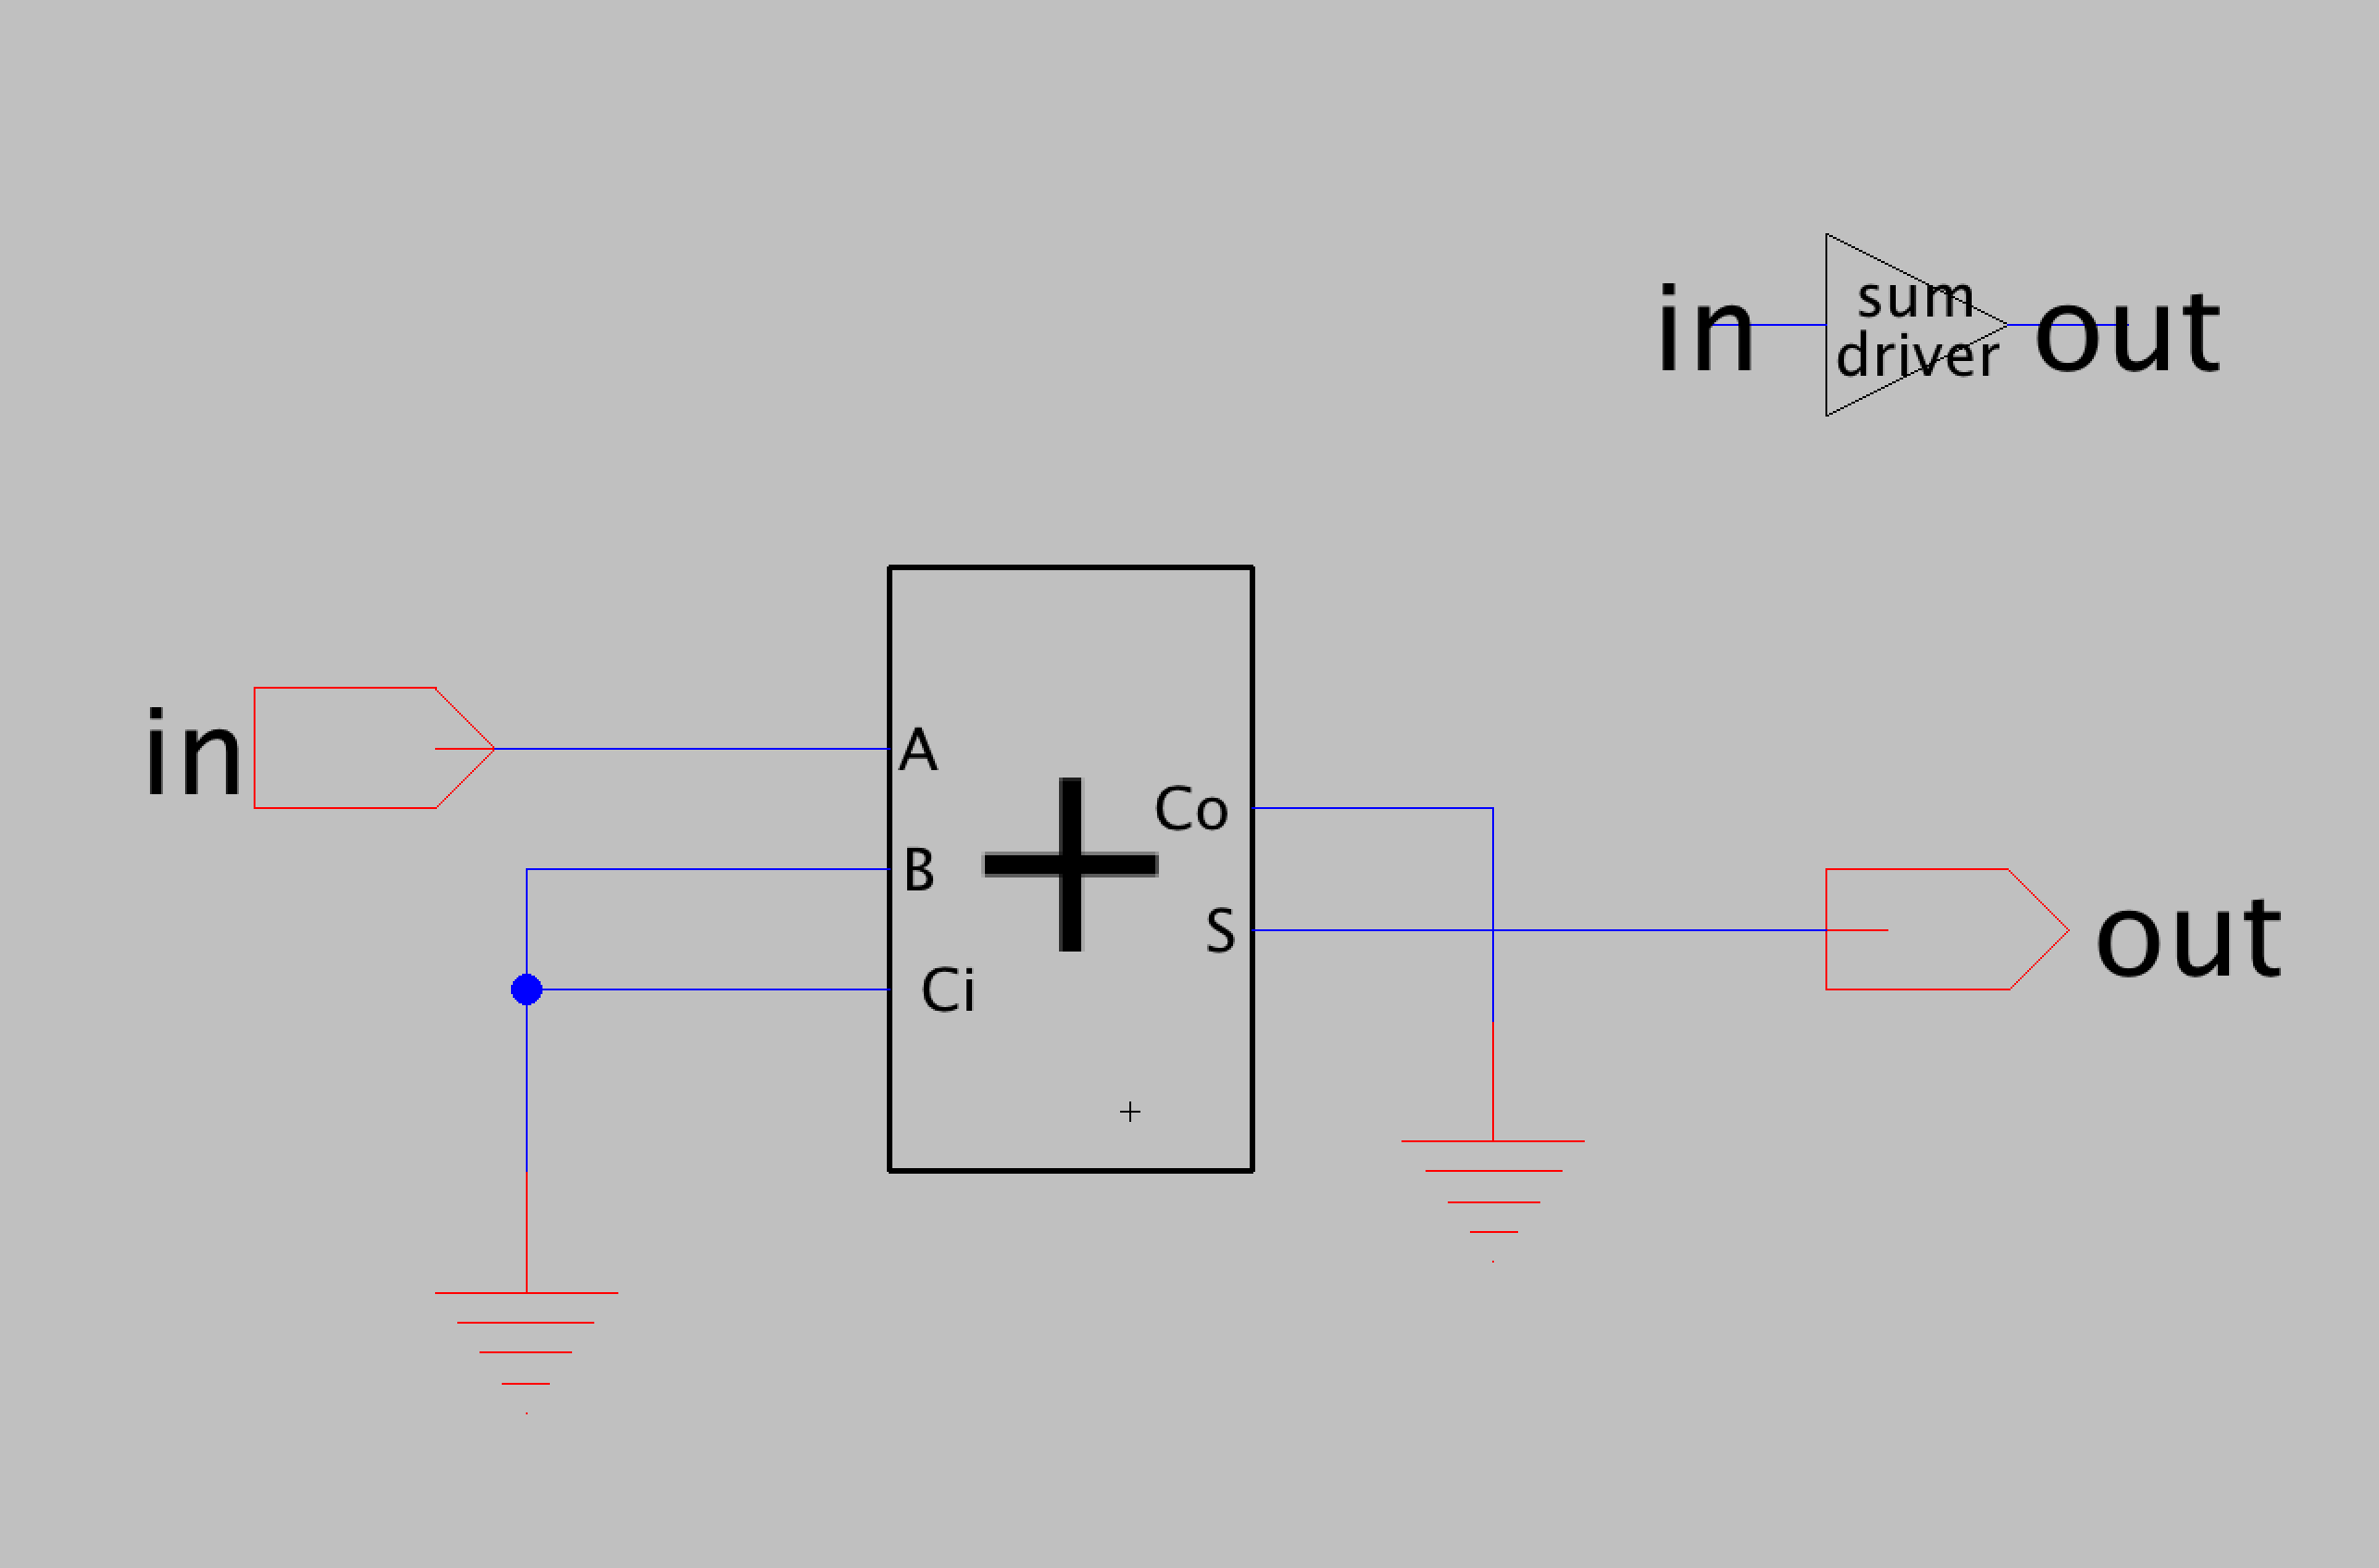
\includegraphics[width=\linewidth]{baseline_screenshots/baseline_sum_driver.png}
  \caption{Schematic for a driver and load based off of the sum cell}
  \label{fig:baseline_sum_driver_sch}
\end{figure}

\begin{figure}[H]
  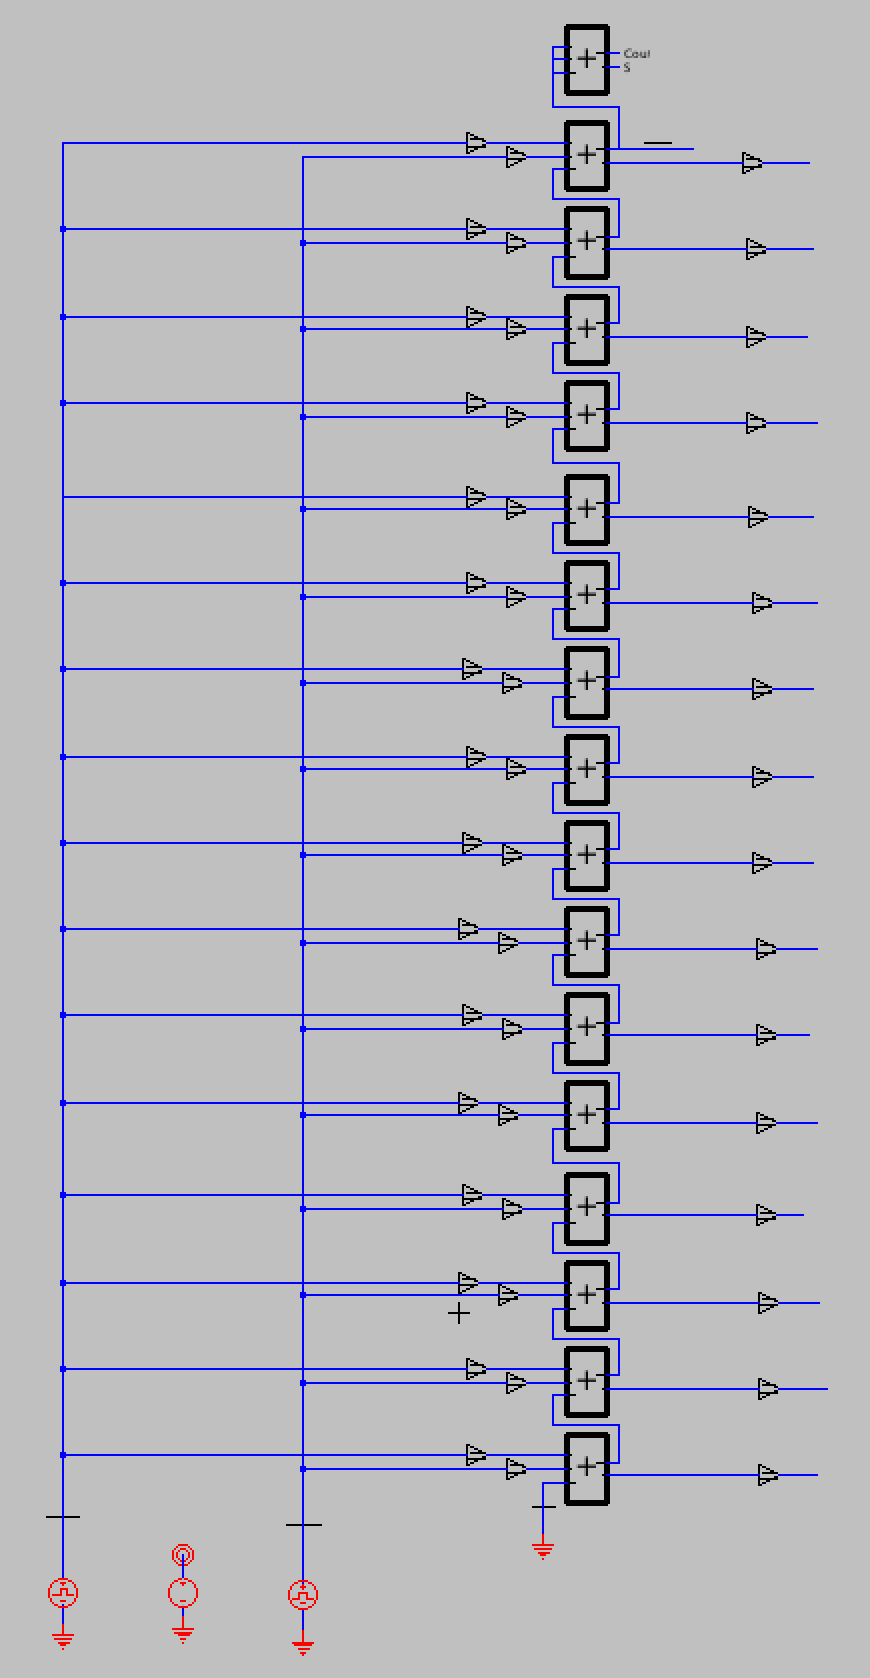
\includegraphics[width=270pt]{baseline_screenshots/entire_adder.png}
  \caption{16bit Adder}
  \label{fig:baseline_16b_adder_sch}
\end{figure}

\begin{figure}[H]
  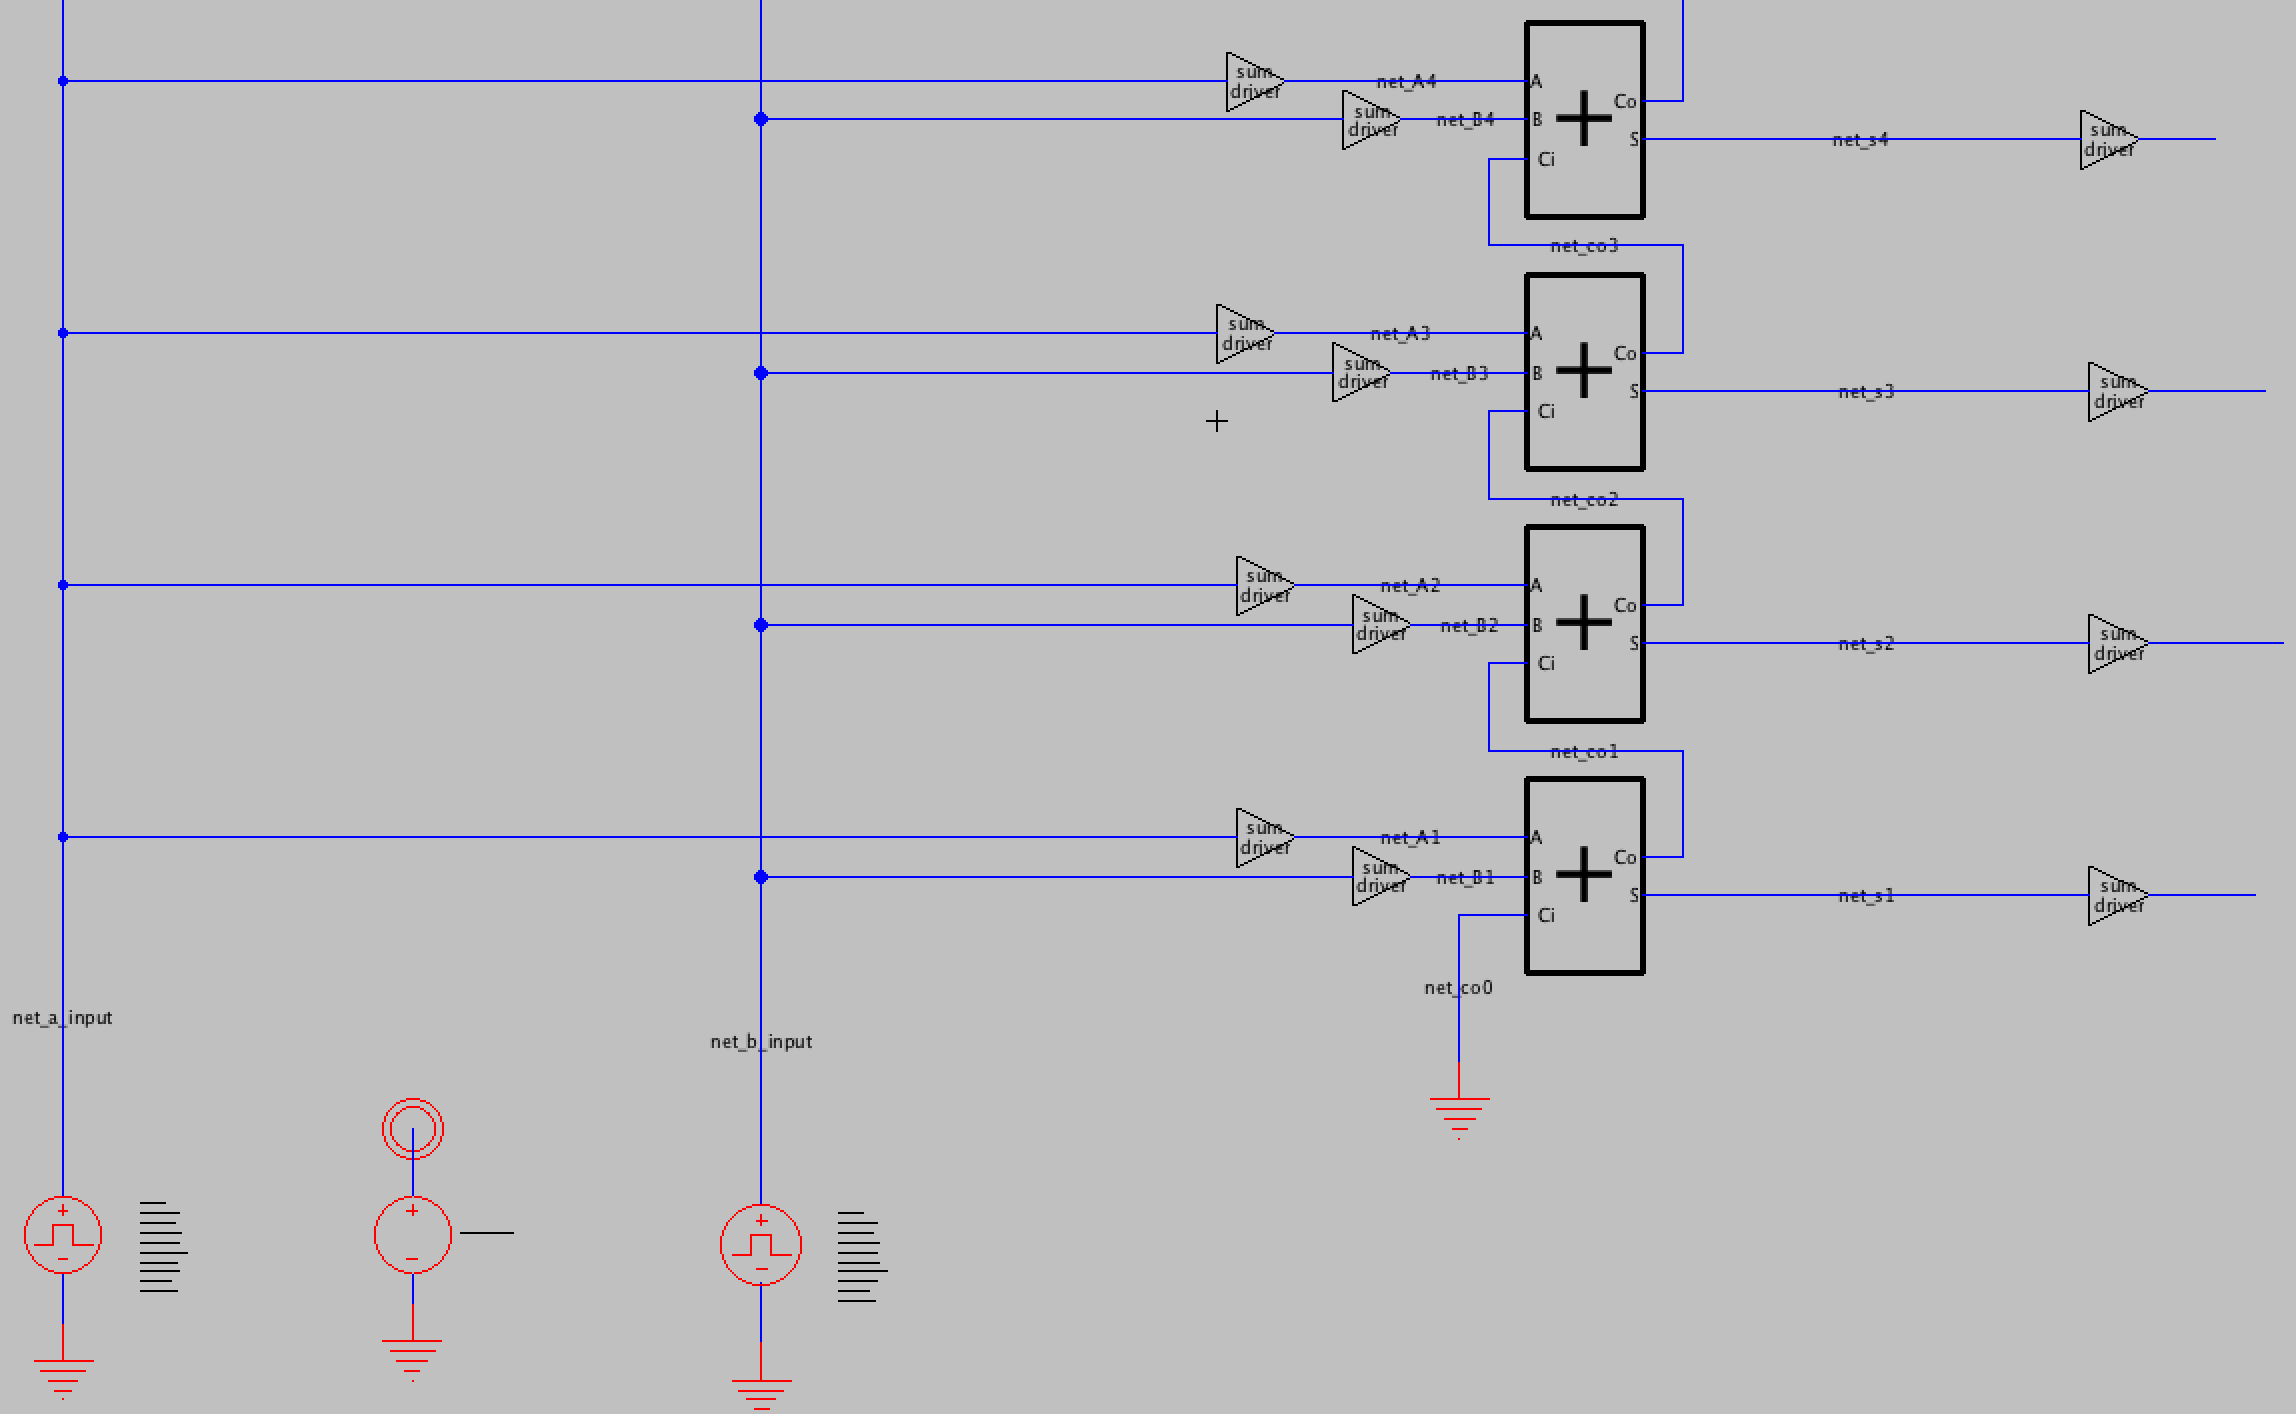
\includegraphics[width=\linewidth]{baseline_screenshots/zoomed_adder.png}
  \caption{Zoom of 16bit Adder}
  \label{fig:baseline_16b_adder_sch_zoomed}
\end{figure}

\subsection{Design Metrics}

\subsubsection{Area}
The XNOR gate has 30 transistors. The baseline bit slice has 2 inverters which each have 2 transistors and the logic for the carry out, which has 12 transistors. In total, since every transistor is width 1 minimum unit, this gives an area of $30 + 2 + 2 + 12 = 46$ units for each bit slice. There are 16 of these, and thus we have the following:\\
$$Area = 16 \times 46 = 736units$$
\subsubsection{Delay}
See above.

\subsubsection{Active Energy}
\textbf{Maximum switching energy} = $(0.582845fW) \times 16 = 9.32552fW$.\\
\textbf{Average switching energy} = $\frac{3.90943fW}{8 inputs} \times 16 = 7.81886fW$

\subsubsection{Leakage Energy}
\begin{enumerate}
\item Minimum leakage energy = $0.507343aW \times 16 = 8.117488aW$
\item Maximum leakage energy = $23.1757aW \times 16 = 370.8112aW$
\end{enumerate}

\subsection{Metric Evaluation}
\textbf{Area}\\
Area was calculated crudely based on the suggested method in the handout. This is noted as crude, but less important for our analysis.\\
\textbf{Delay}\\
Delay was calculated with the $\tau$ approximation and measured in ngspice. The delay was only measured from the start of the input to the final rise of the last carry out since that is the longest path through the adder.\\
\textbf{Active Energy}\\
\textit{Maximum switching energy} was evaluated by the schematic in Figure \ref{fig:baseline_energy_sch} and was found to be the case when the inputs switched from $(A, B, C) = (0 \rightarrow 1, 0, 0)$. To do this, I evaluated the 8 possible cases and multiplied by 16 because of the 16 gates dissipating energy. \\
\textit{Average switching energy} was evaluated by the schematic in Figure \ref{fig:baseline_energy_sch}. For this evaluation, I integrated over the entire input sequence from all 0 inputs to all 1 inputs and divided by the number of inputs. This gives the average energy dissipation for a single bit slice given a random selection of inputs. I also multiplied this by 16 to model the entire adder's energy dissipation.\\
\textbf{Leakage Energy}\\
Both maximum and minimum leakage energy were found by plotting the current into a single-bit adder (Figure \ref{fig:baseline_leakage_energy} and \ref{fig:baseline_leakage_energy_zoom}). As one can see, the minimum occurs when all inputs are high and the maximum occurs around $0.8ns$, which is the input case $(A, B, C) = (0, 1, 1)$.

\begin{figure}[H]
  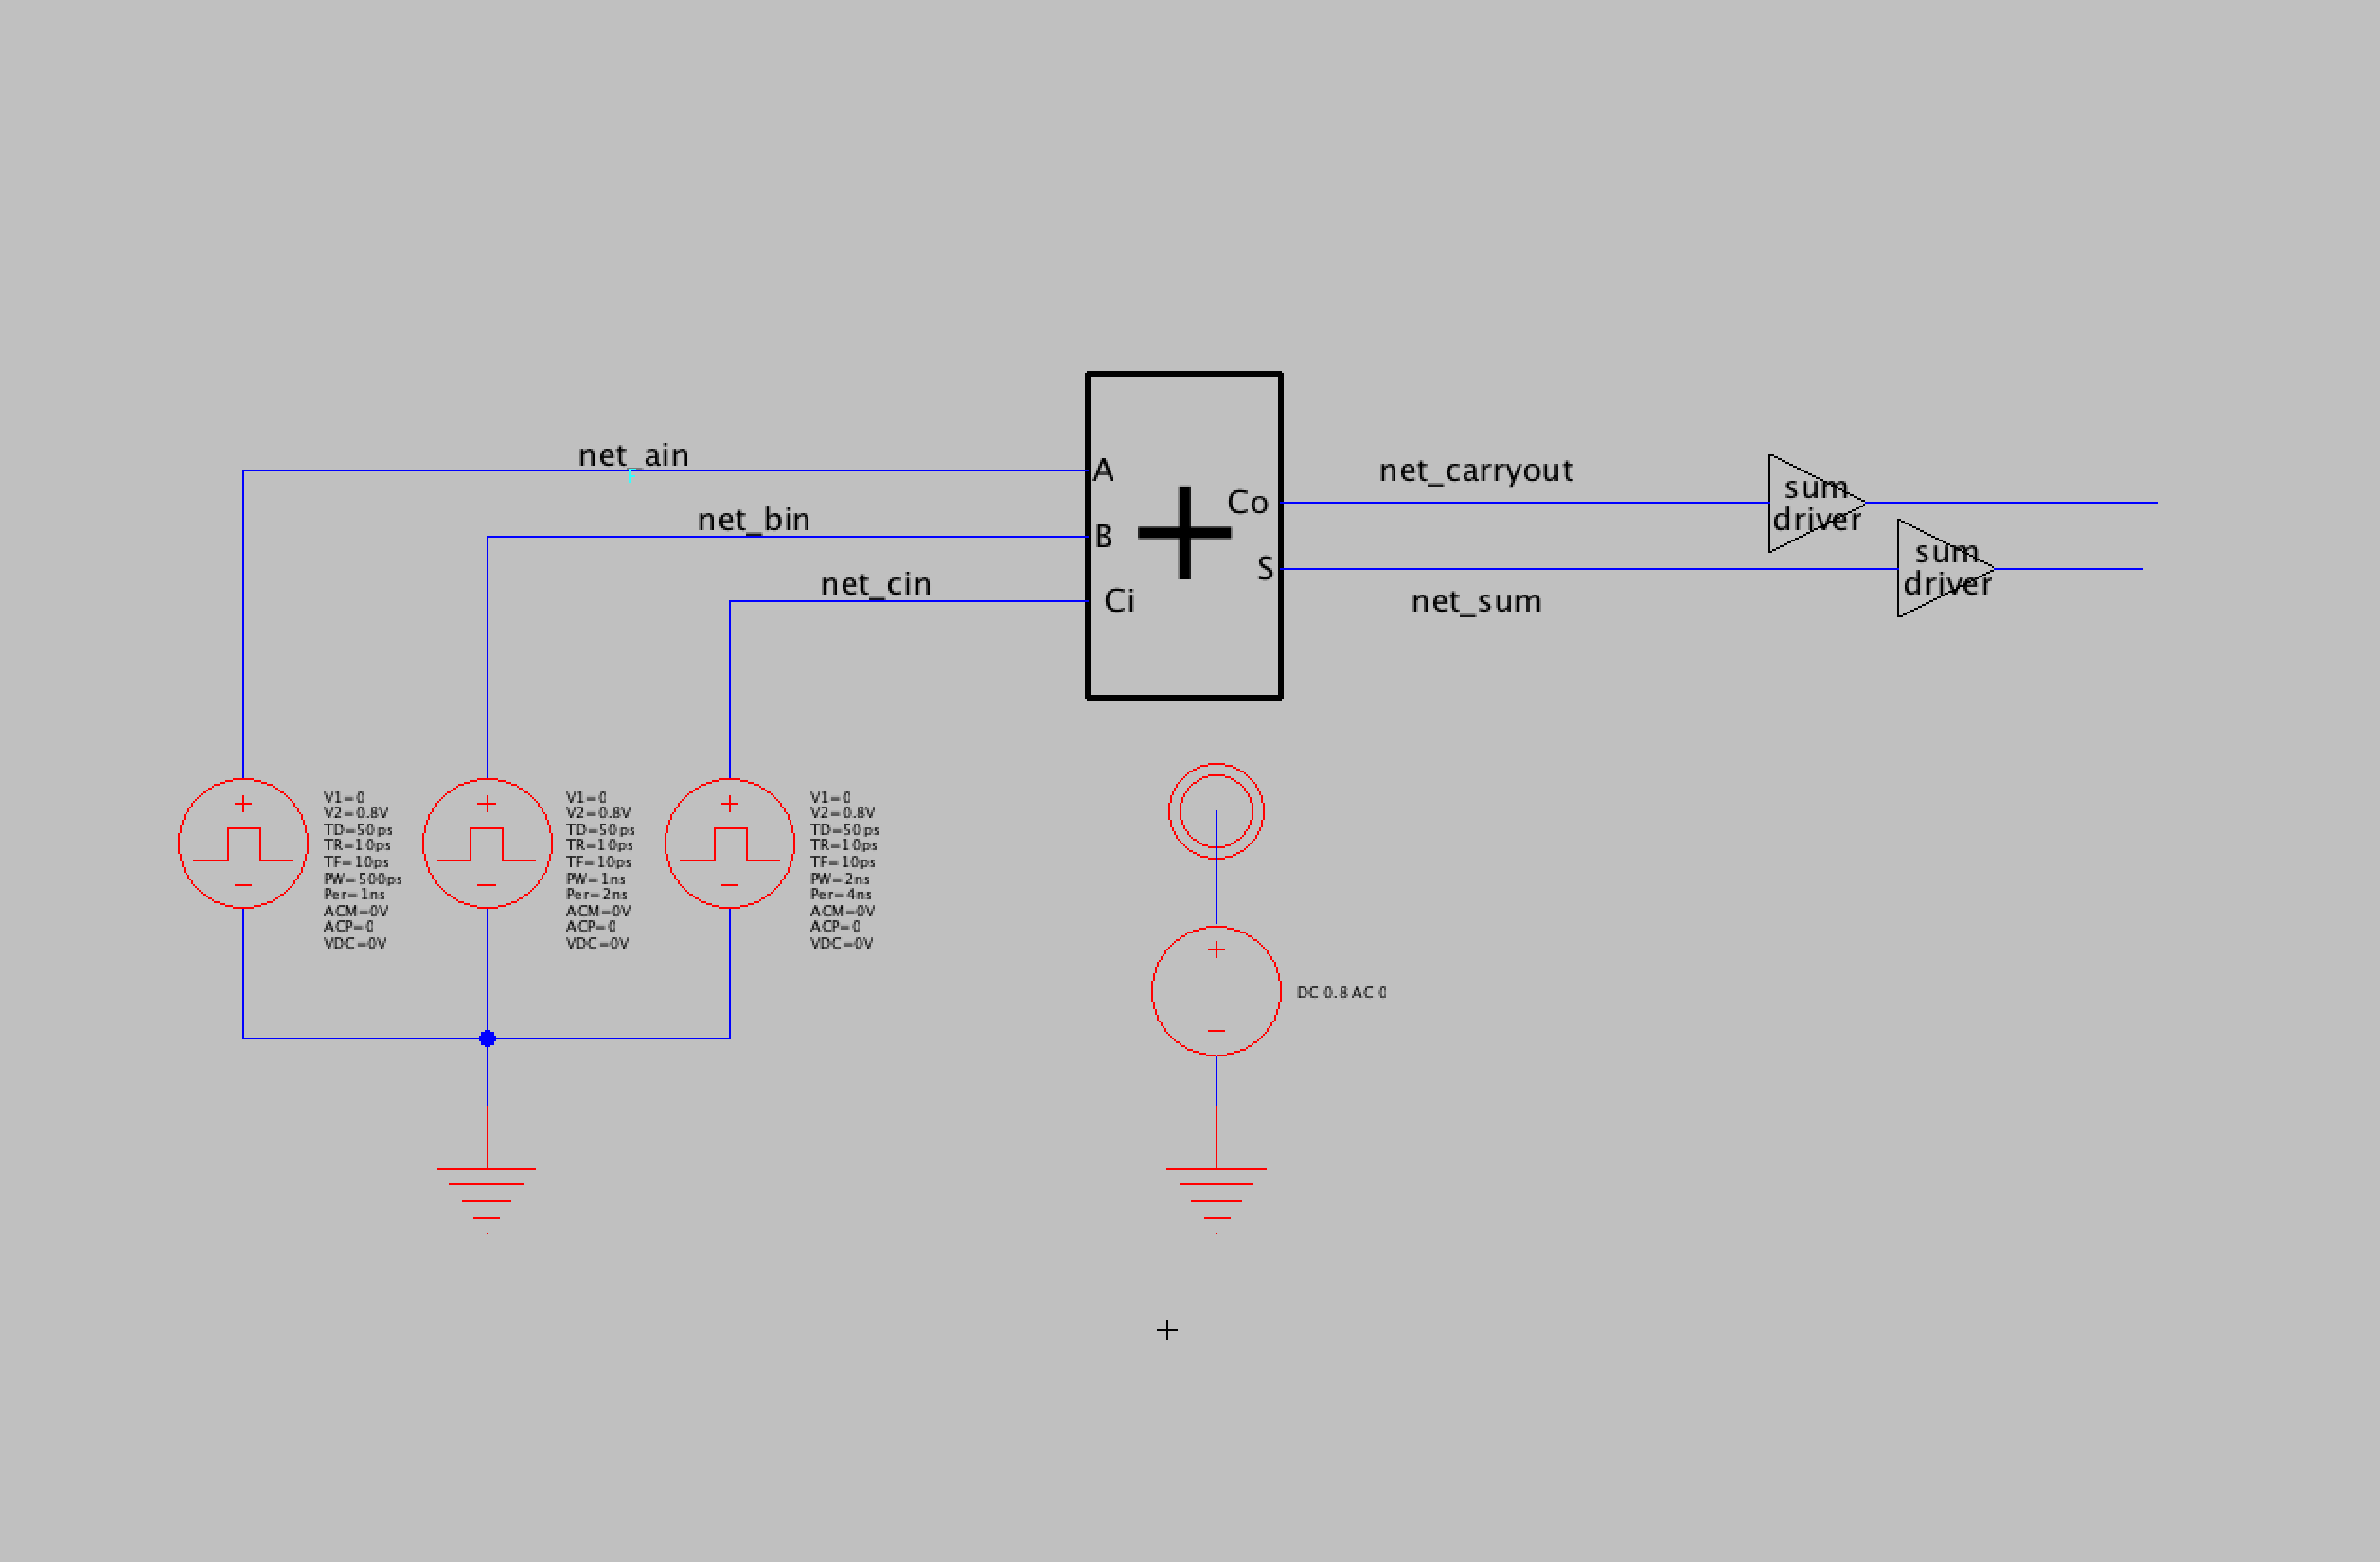
\includegraphics[width=\linewidth]{baseline_screenshots/baseline_test_power_sch.png}
  \caption{Schematic for evaluating energy requirement}
  \label{fig:baseline_energy_sch}
\end{figure}
\begin{figure}[H]
  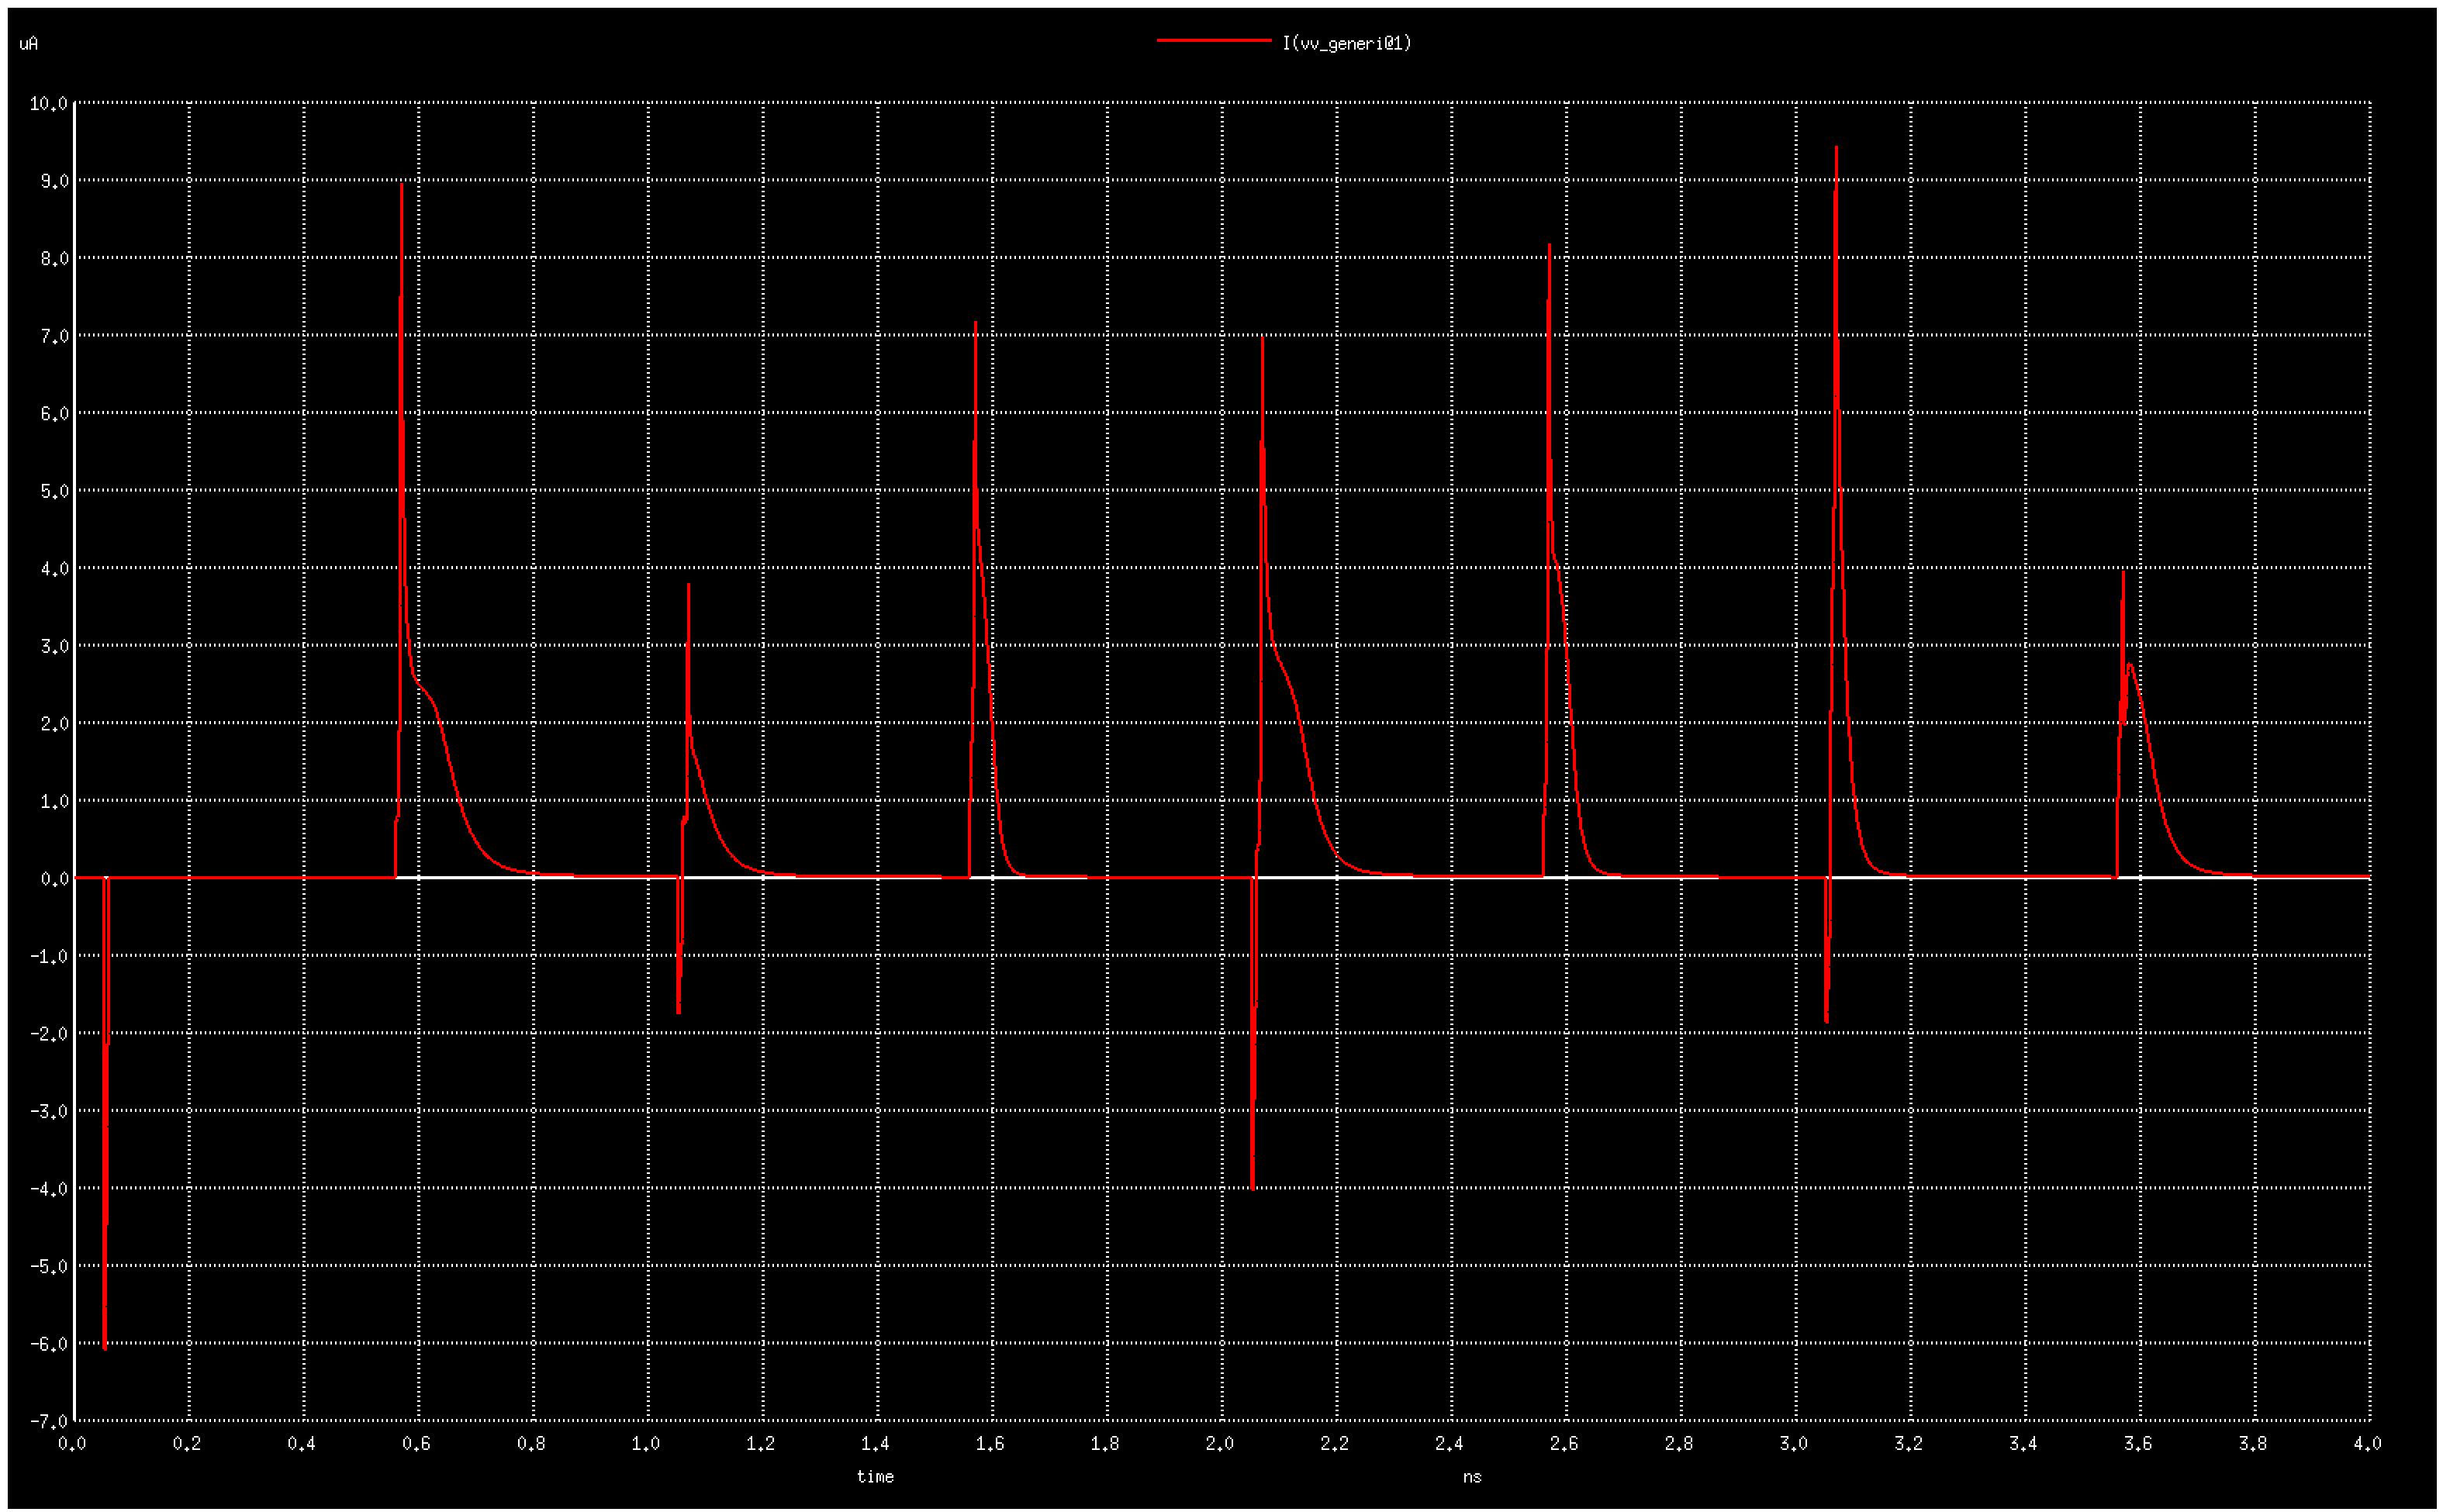
\includegraphics[width=\linewidth]{baseline_screenshots/baseline_leakage_energy.png}
  \caption{Simulation of current through adder}
  \label{fig:baseline_leakage_energy}
\end{figure}
\begin{figure}[H]
  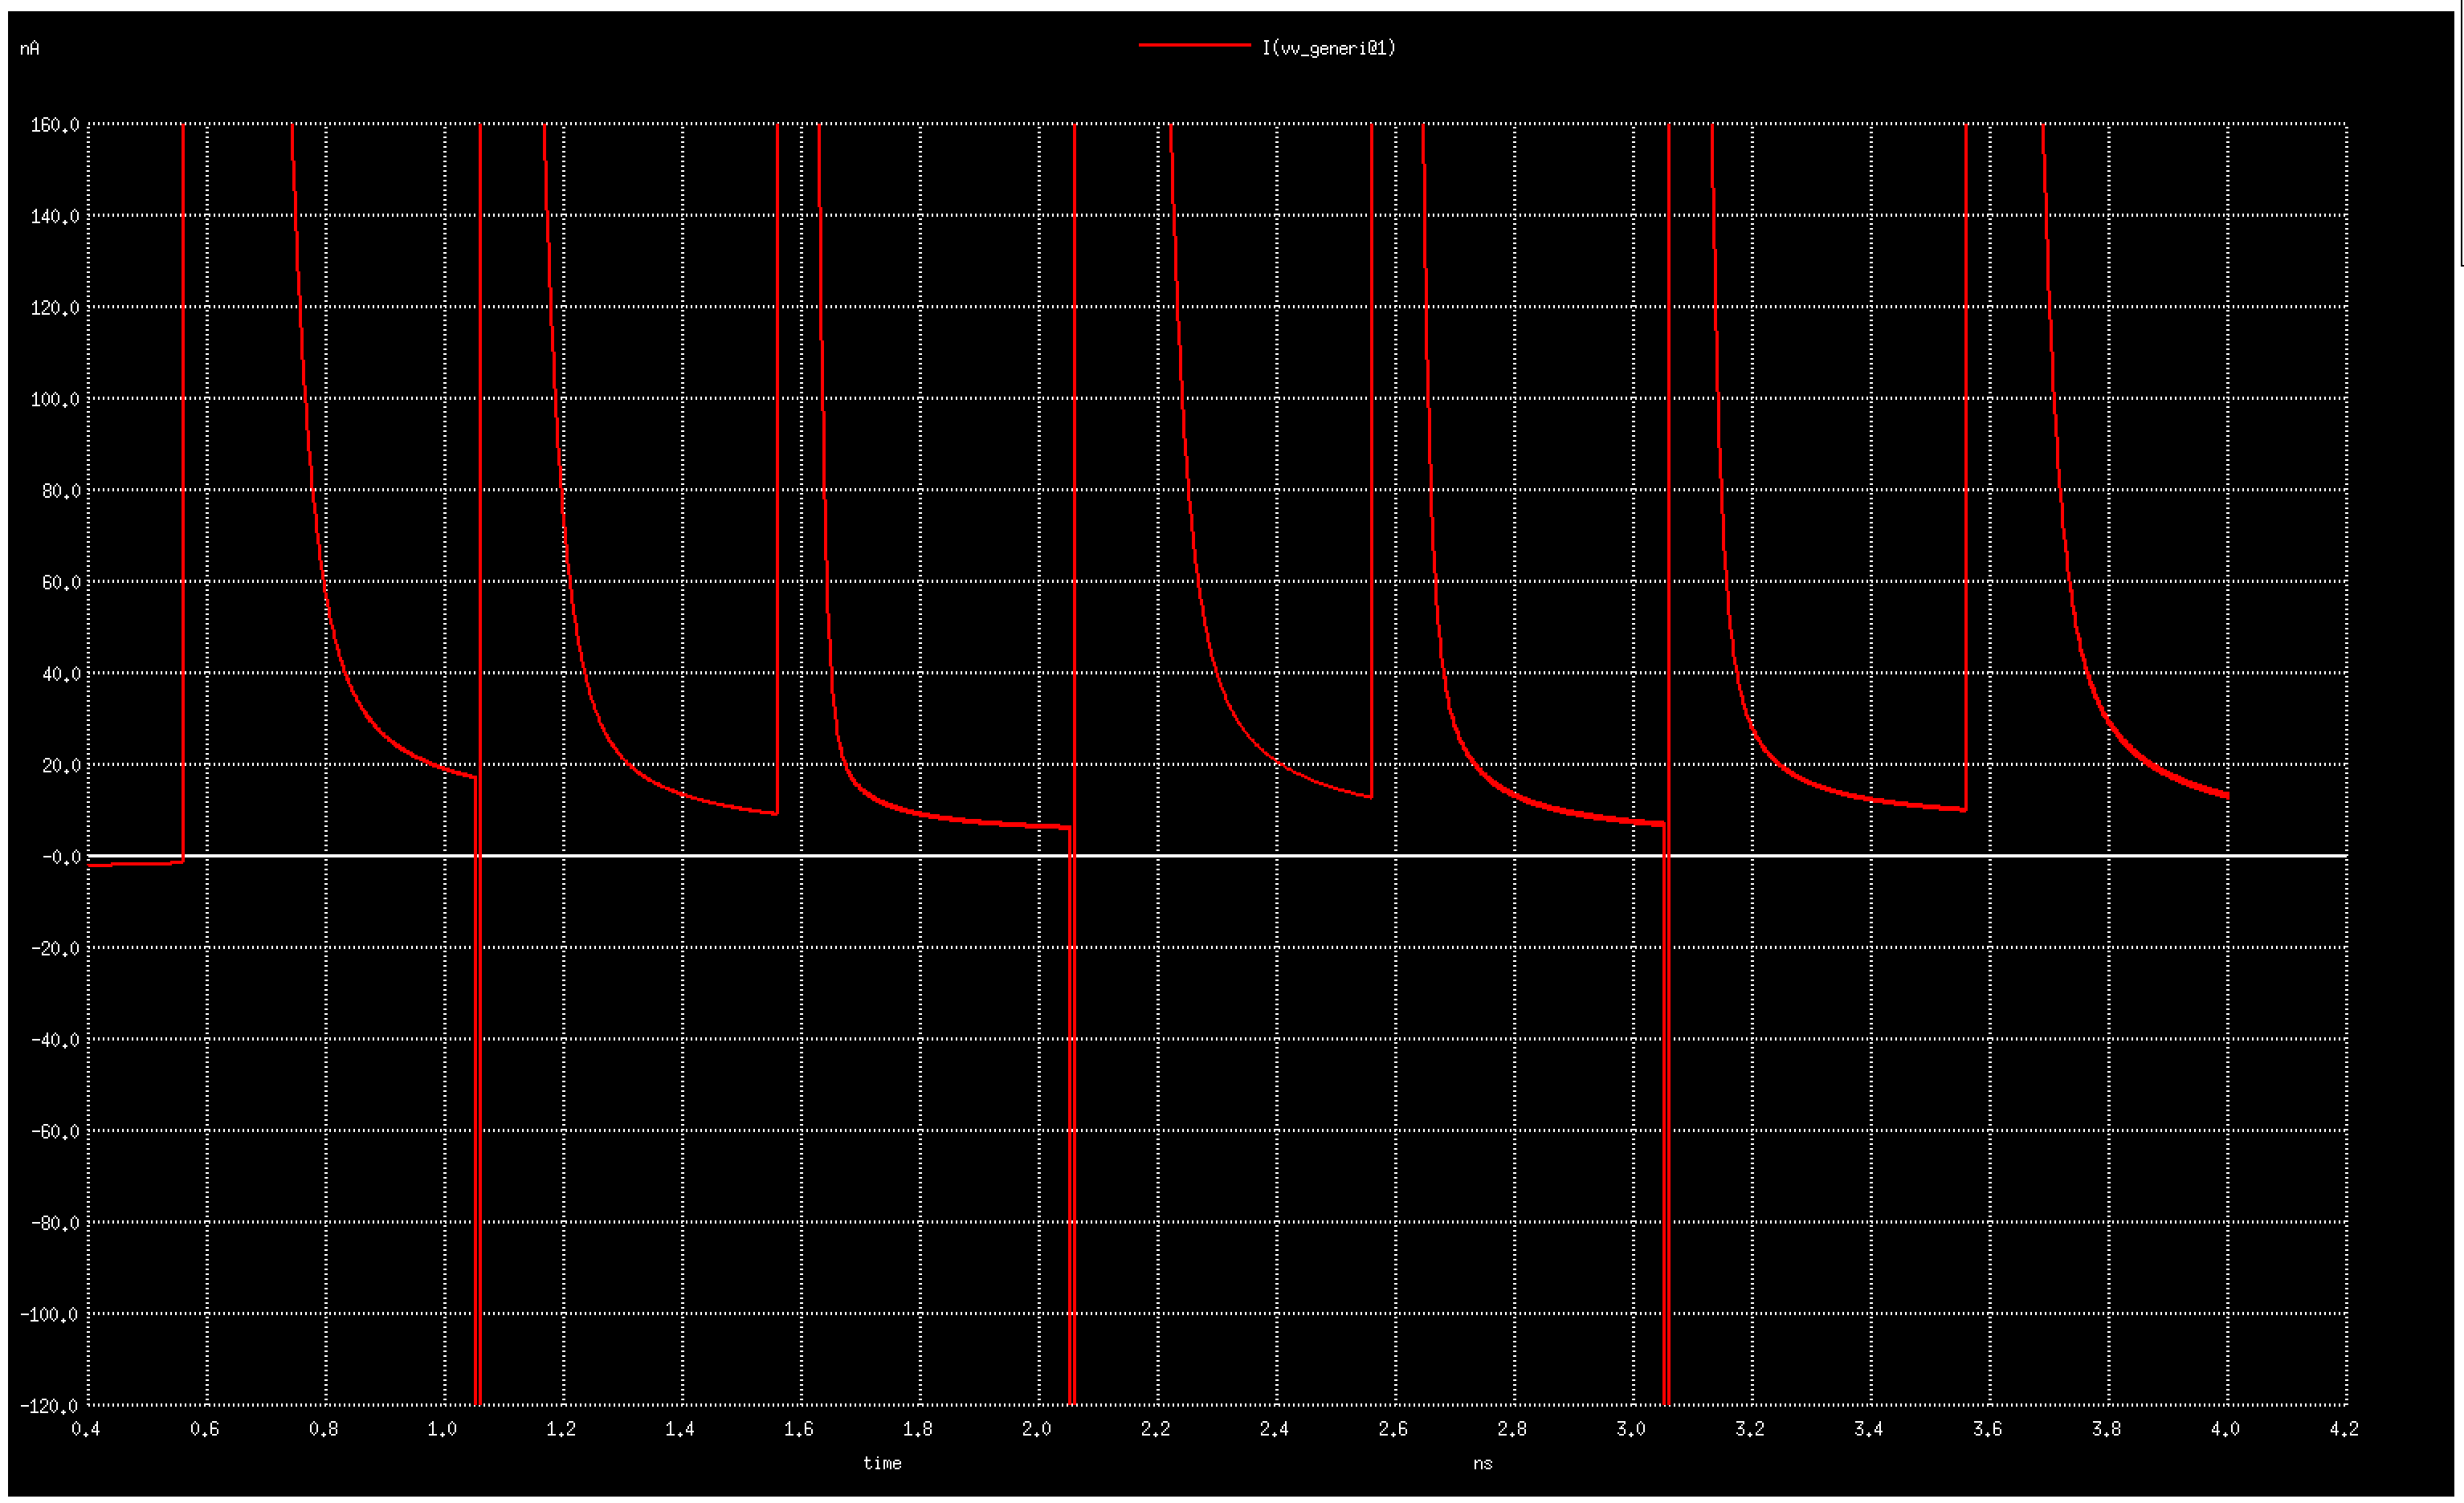
\includegraphics[width=\linewidth]{baseline_screenshots/baseline_leakage_energy_zoom.png}
  \caption{Zoomed simulation of current through adder}
  \label{fig:baseline_leakage_energy_zoom}
\end{figure}

\pagebreak

\section{Optimized Design}
The optimized design has four components, which are built into two different 1-bit adders. They will be referenced as Carry (Figure \ref{fig:opt_carry_sch}), nCarry (Figure \ref{fig:opt_ncarry_sch}), Sum (Figure \ref{fig:opt_sum_sch}), and nSum (Figure \ref{fig:opt_nsum_sch}), which combine to build a 1-bit Adder (Figure \ref{fig:opt_1b_adder_sch}) and a 1-bit nAdder (Figure \ref{fig:opt_1b_nadder_sch}). Those adders are cascaded to complete the full 16-bit Adder (Figure \ref{fig:opt_16b_adder_sch}, Figure \ref{fig:opt_16b_adder_sch_zoom1}, Figure \ref{fig:opt_16b_adder_sch_zoom2})The prefix $n$ indicates that the module takes as an input $\overline{C}$ as opposed to $C$. The equations for the outputs are as follows:\\
\textbf{Sum:}\\
$$S = \overline{A \xor \overline{(B \xor C_{in}})}$$
\textbf{nSum:}\\
$$S = \overline{A \xor (B \xor \overline{C_{in}})}$$
\textbf{Carry:} (consumes the carry in and generates the compliment of the carry out)\\
$$\overline{C_{out}} = AB + ACin + BCin$$
\textbf{nCarry:} (consumes the compliment of the carry in and generates the carry out)\\
$$C_{out} = \overline{A}\textnormal{ }\overline{B} + \overline{A}\textnormal{ }\overline{C_{in}} + \overline{B}\textnormal{ }\overline{C_{in}}$$

\begin{figure}[H]
  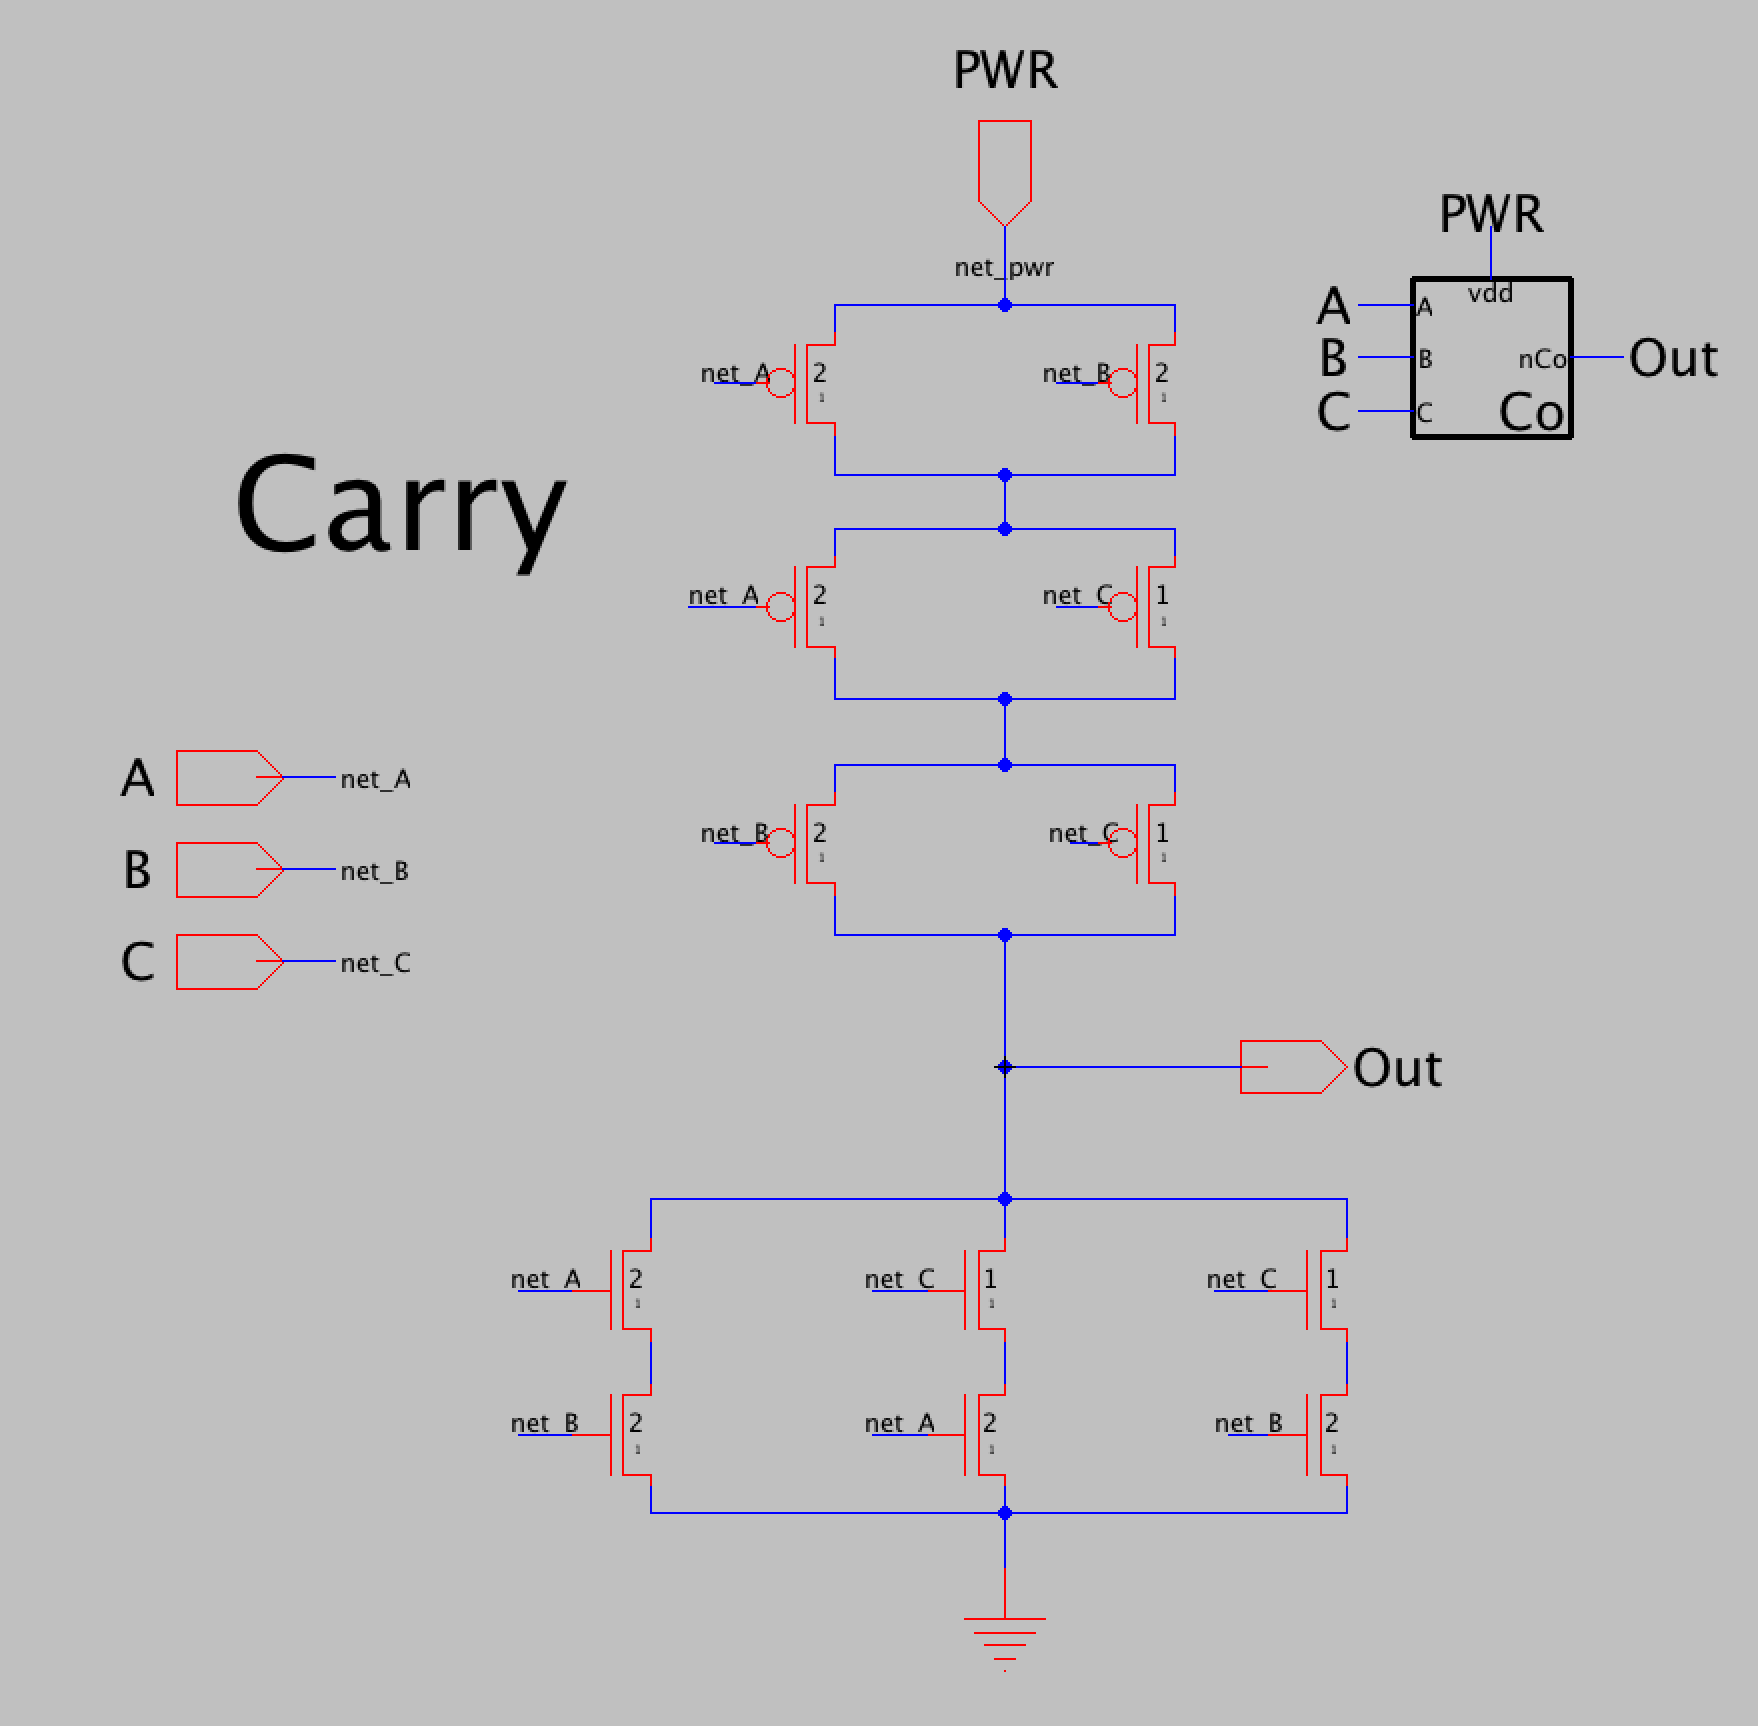
\includegraphics[width=\linewidth]{opt_screenshots/opt_carry_sch.png}
  \caption{Schematic for Optimized Carry}
  \label{fig:opt_carry_sch}
\end{figure}

\begin{figure}[H]
  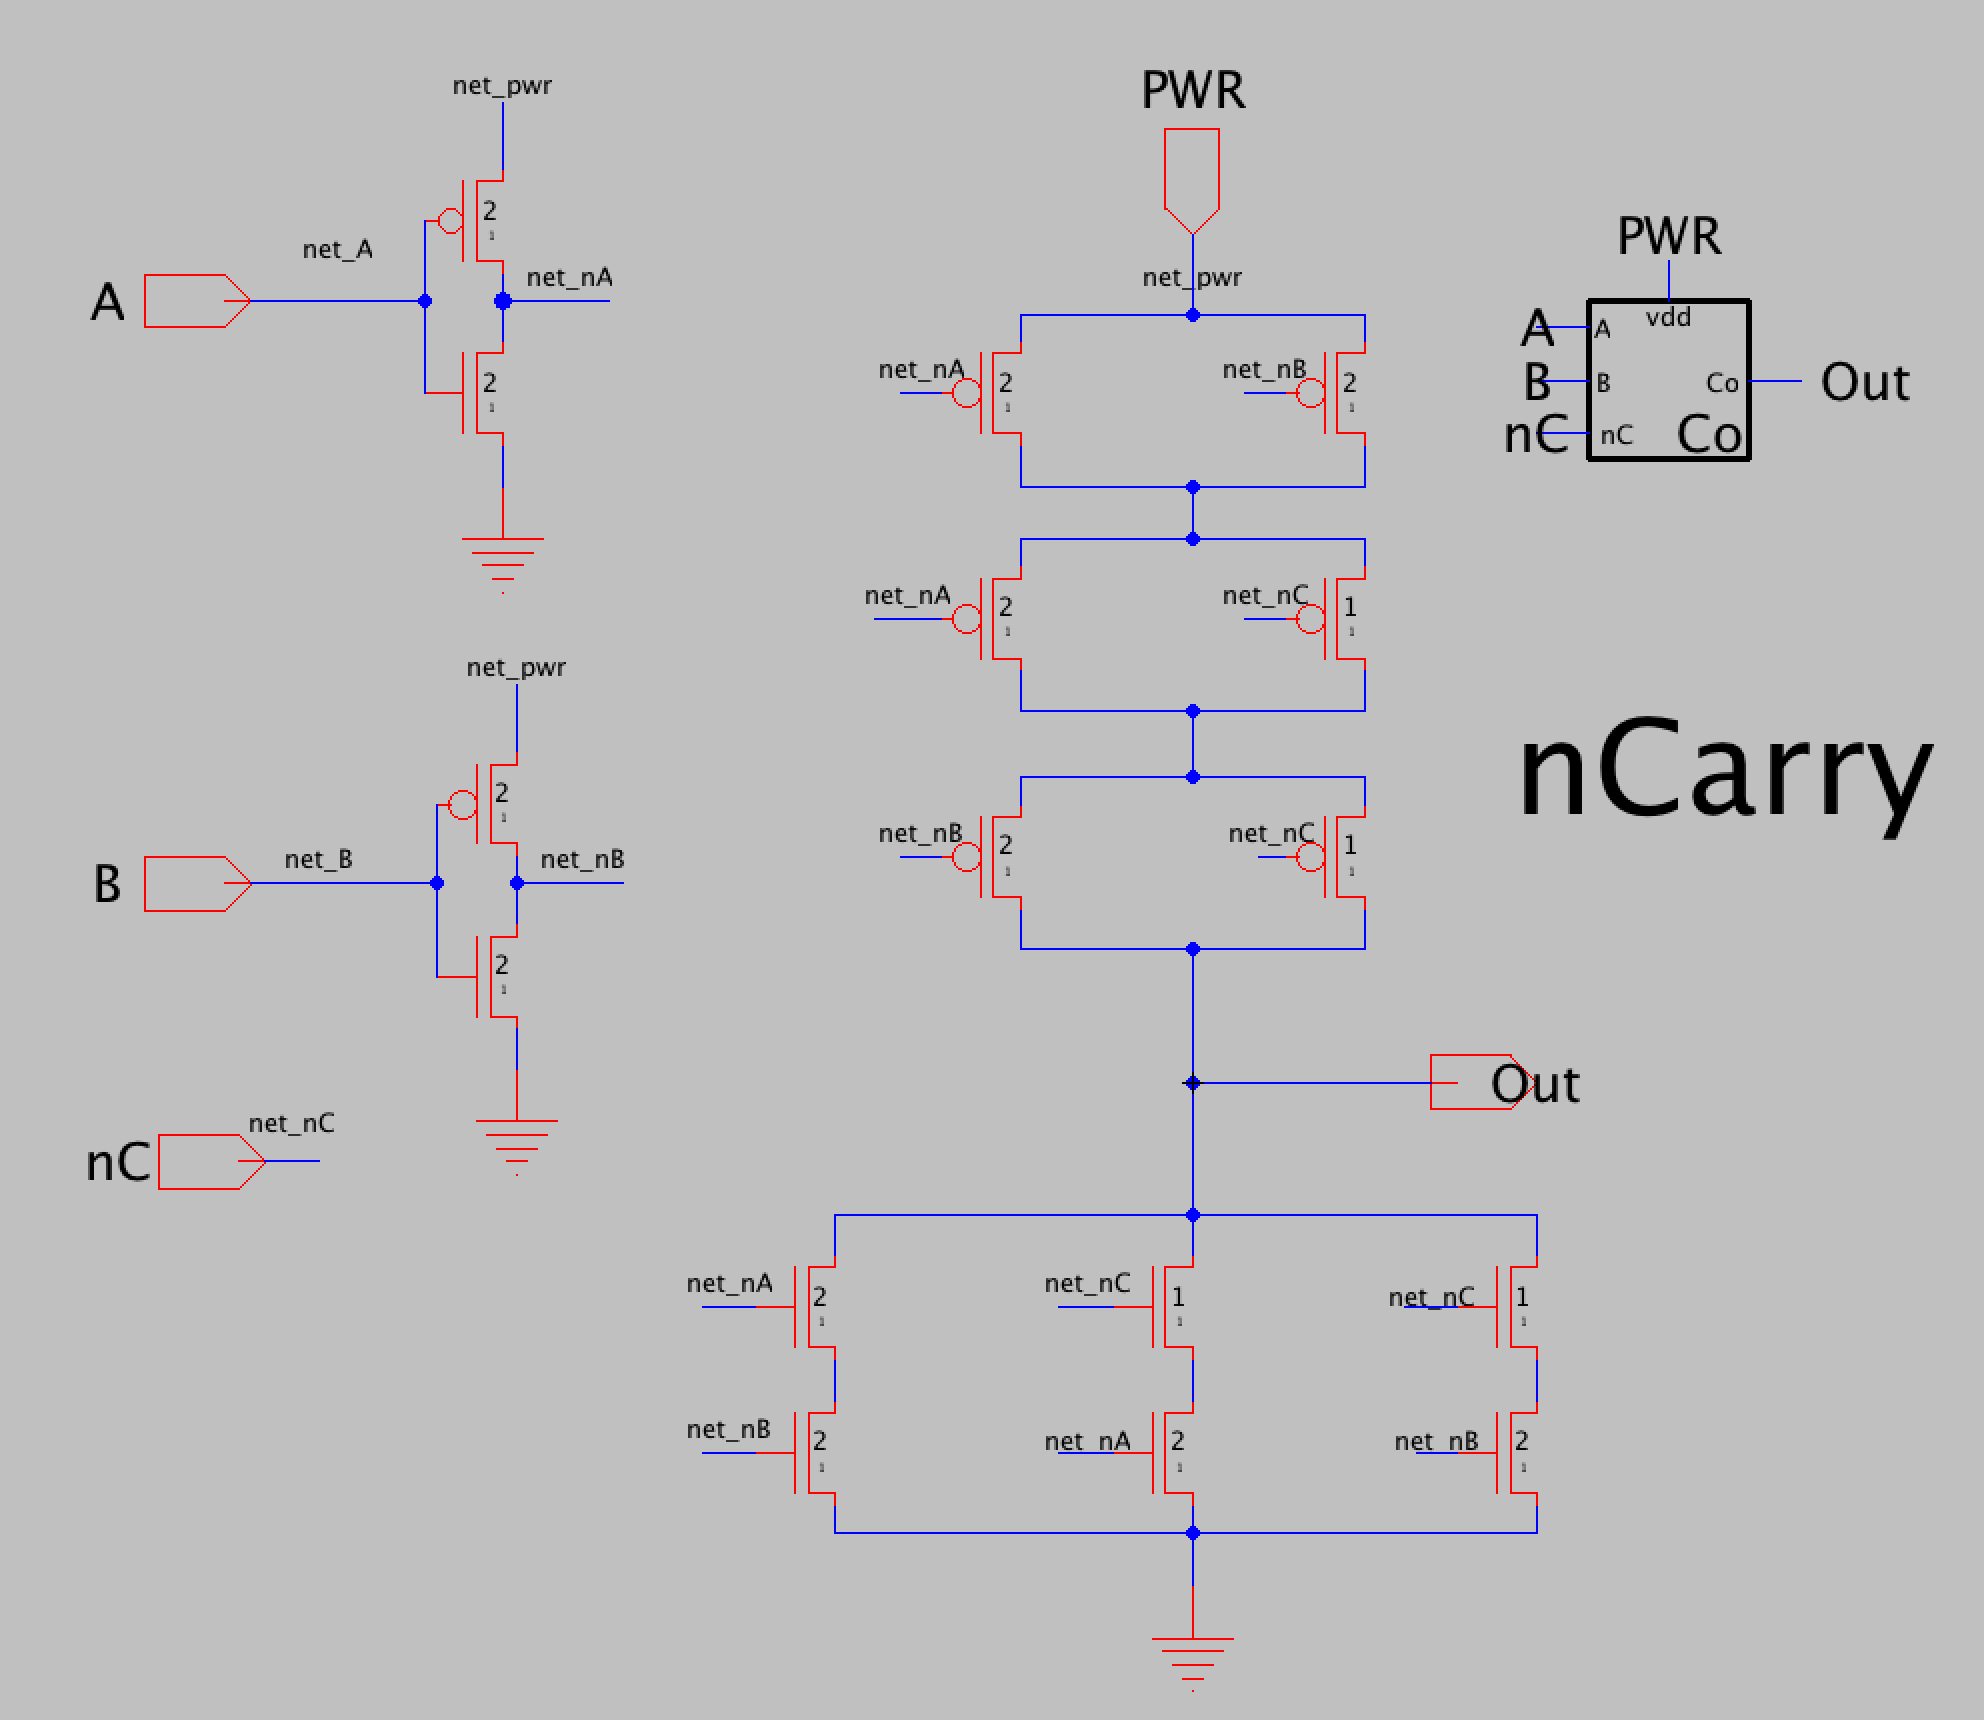
\includegraphics[width=\linewidth]{opt_screenshots/opt_ncarry_sch.png}
  \caption{Schematic for Optimized nCarry}
  \label{fig:opt_ncarry_sch}
\end{figure}

\begin{figure}[H]
  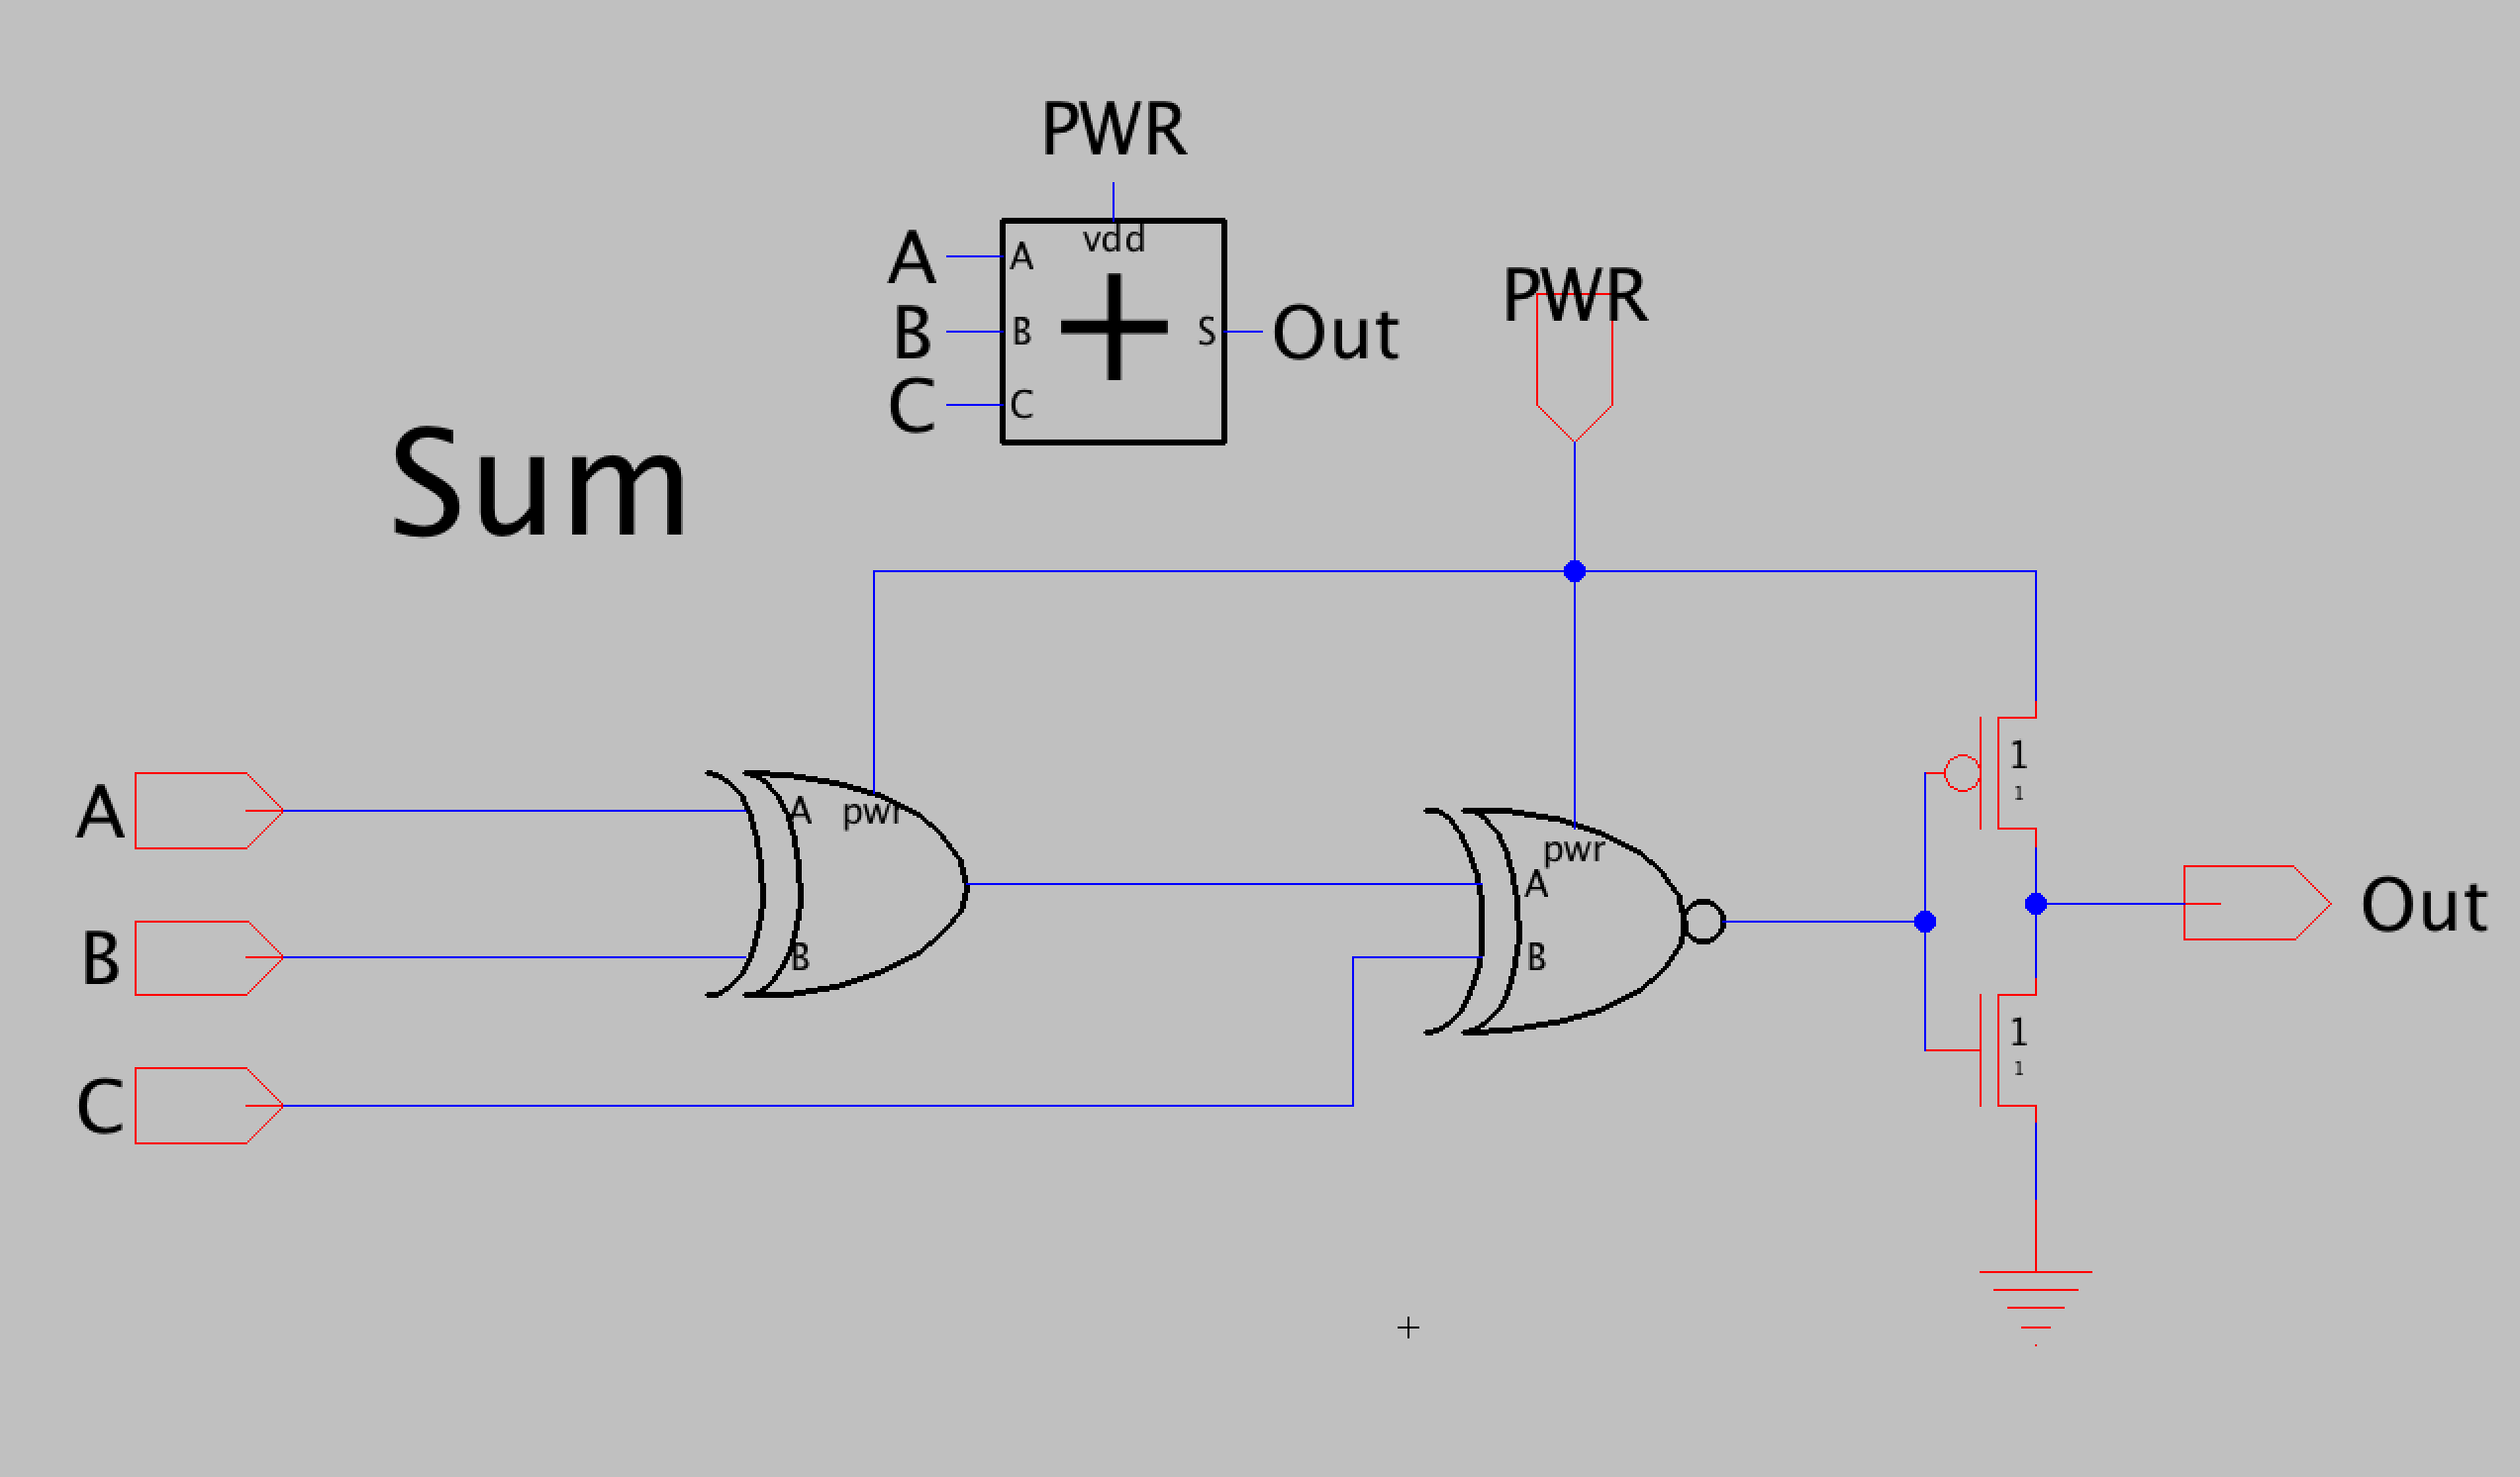
\includegraphics[width=\linewidth]{opt_screenshots/opt_sum_sch.png}
  \caption{Schematic for Optimized Sum}
  \label{fig:opt_sum_sch}
\end{figure}

\begin{figure}[H]
  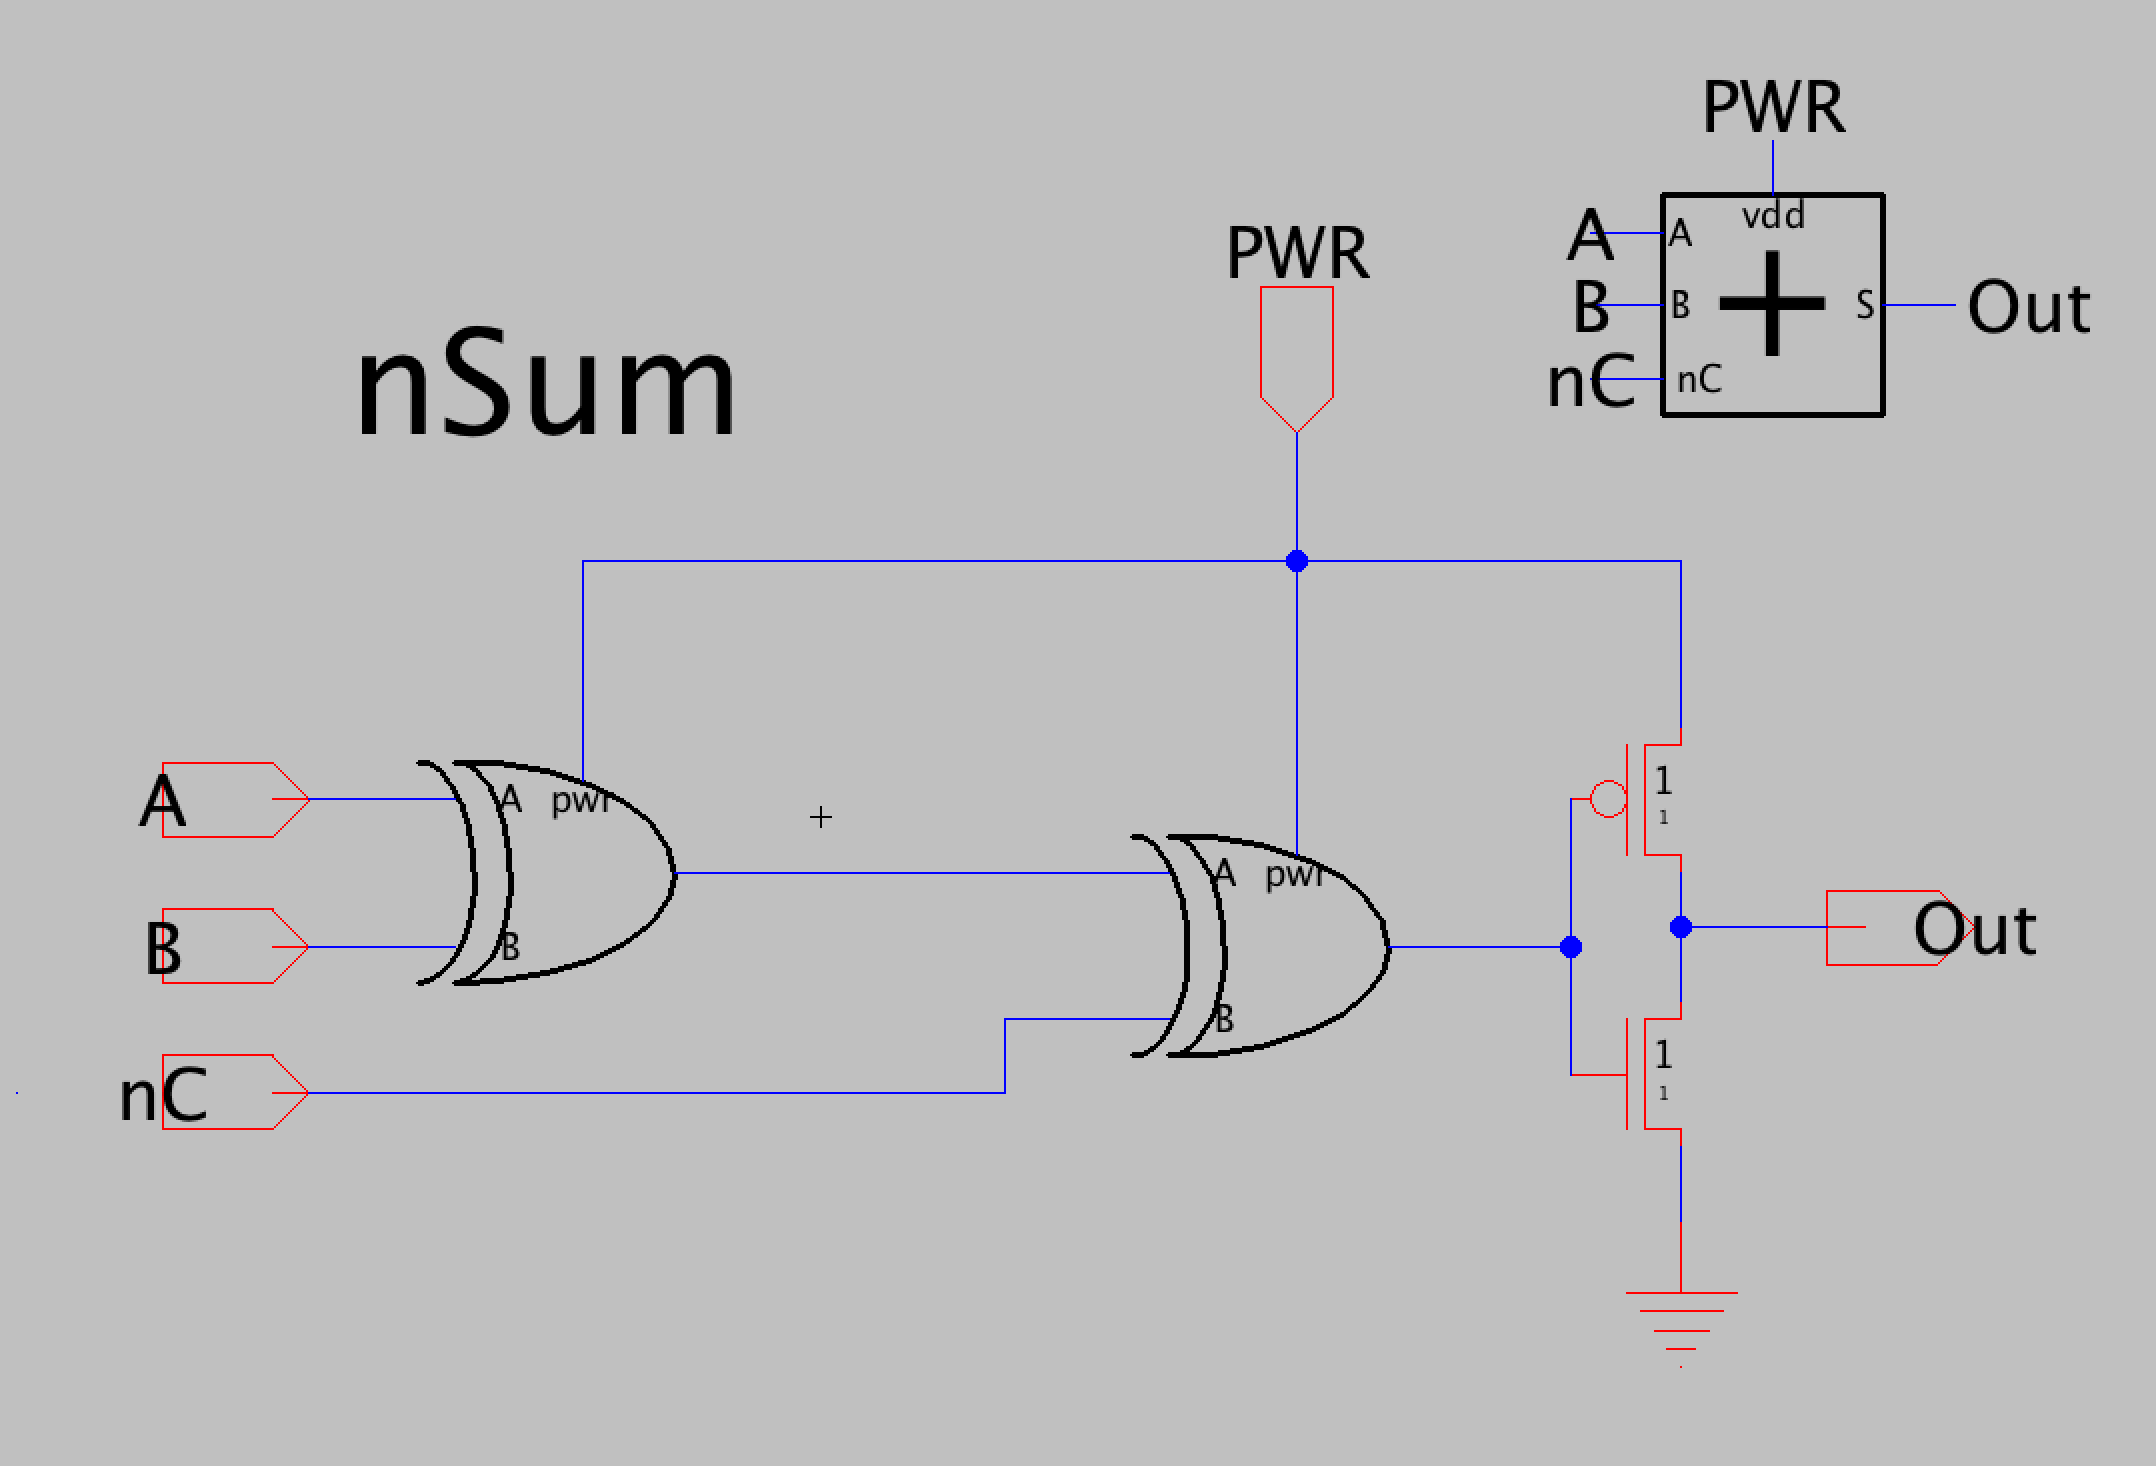
\includegraphics[width=\linewidth]{opt_screenshots/opt_nsum_sch.png}
  \caption{Schematic for Optimized nSum}
  \label{fig:opt_nsum_sch}
\end{figure}

\begin{figure}[H]
  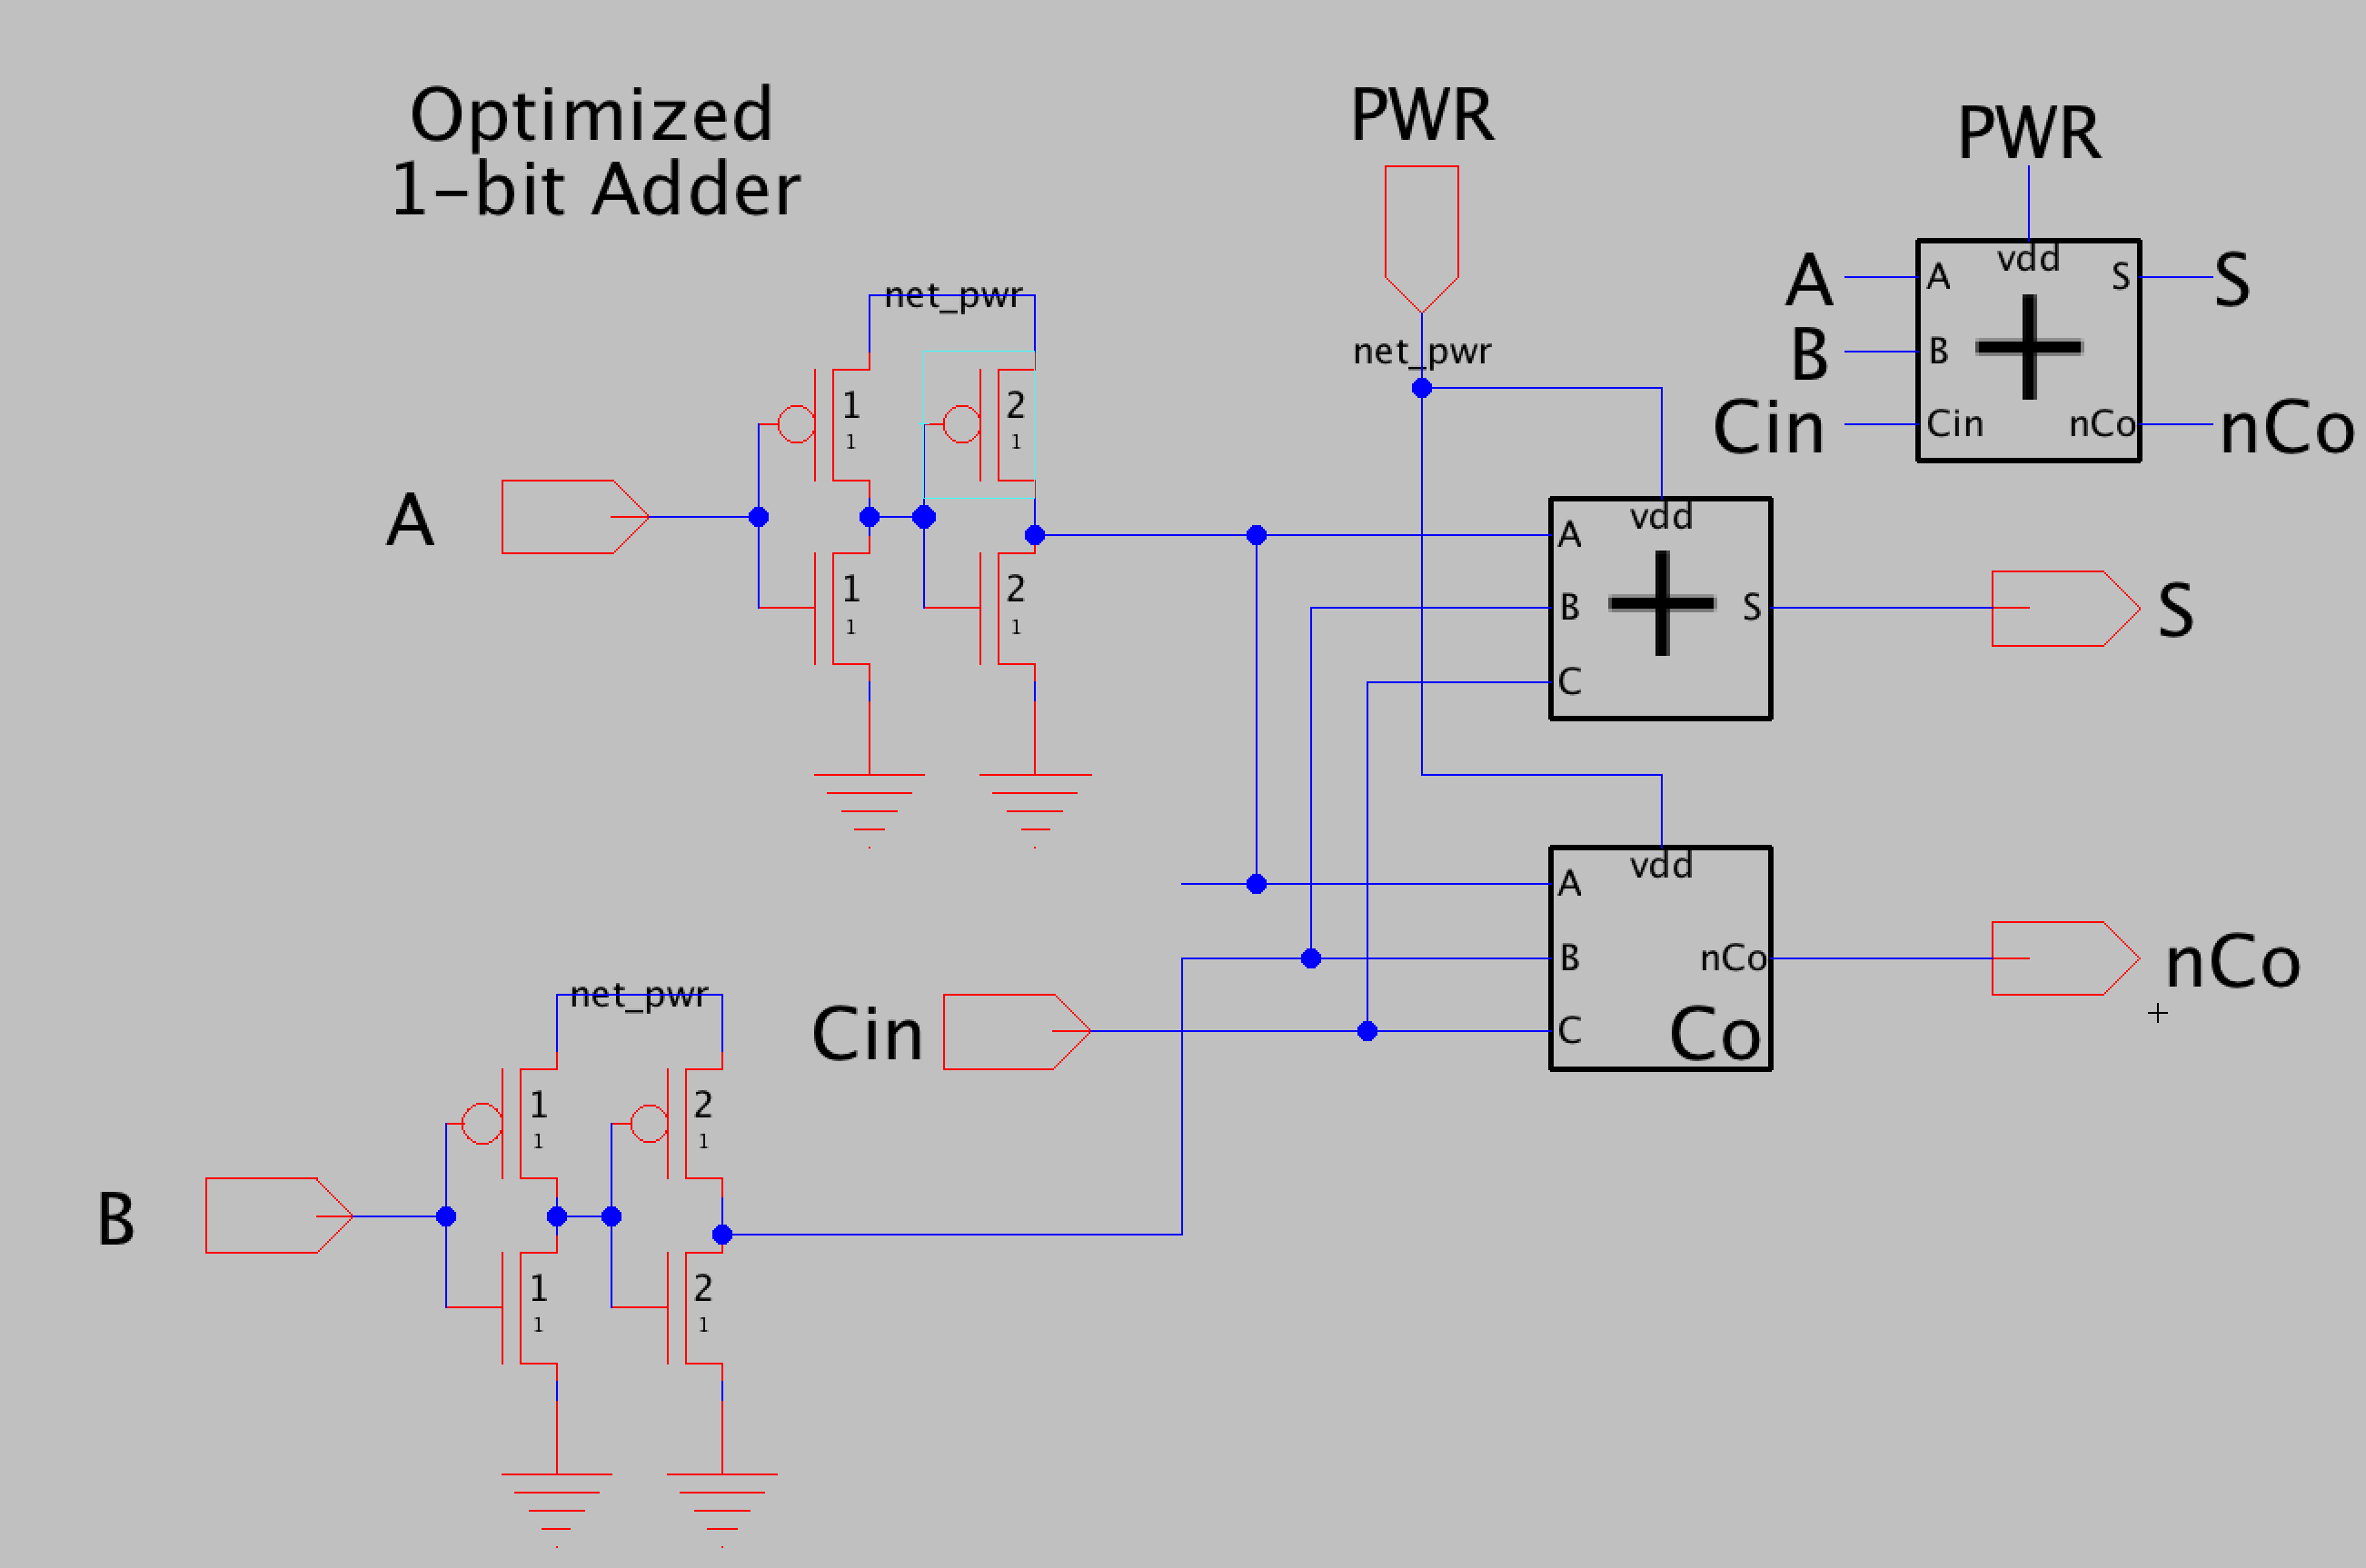
\includegraphics[width=\linewidth]{opt_screenshots/opt_1b_adder_sch.png}
  \caption{Schematic for 1-b Adder}
  \label{fig:opt_1b_adder_sch}
\end{figure}

\begin{figure}[H]
  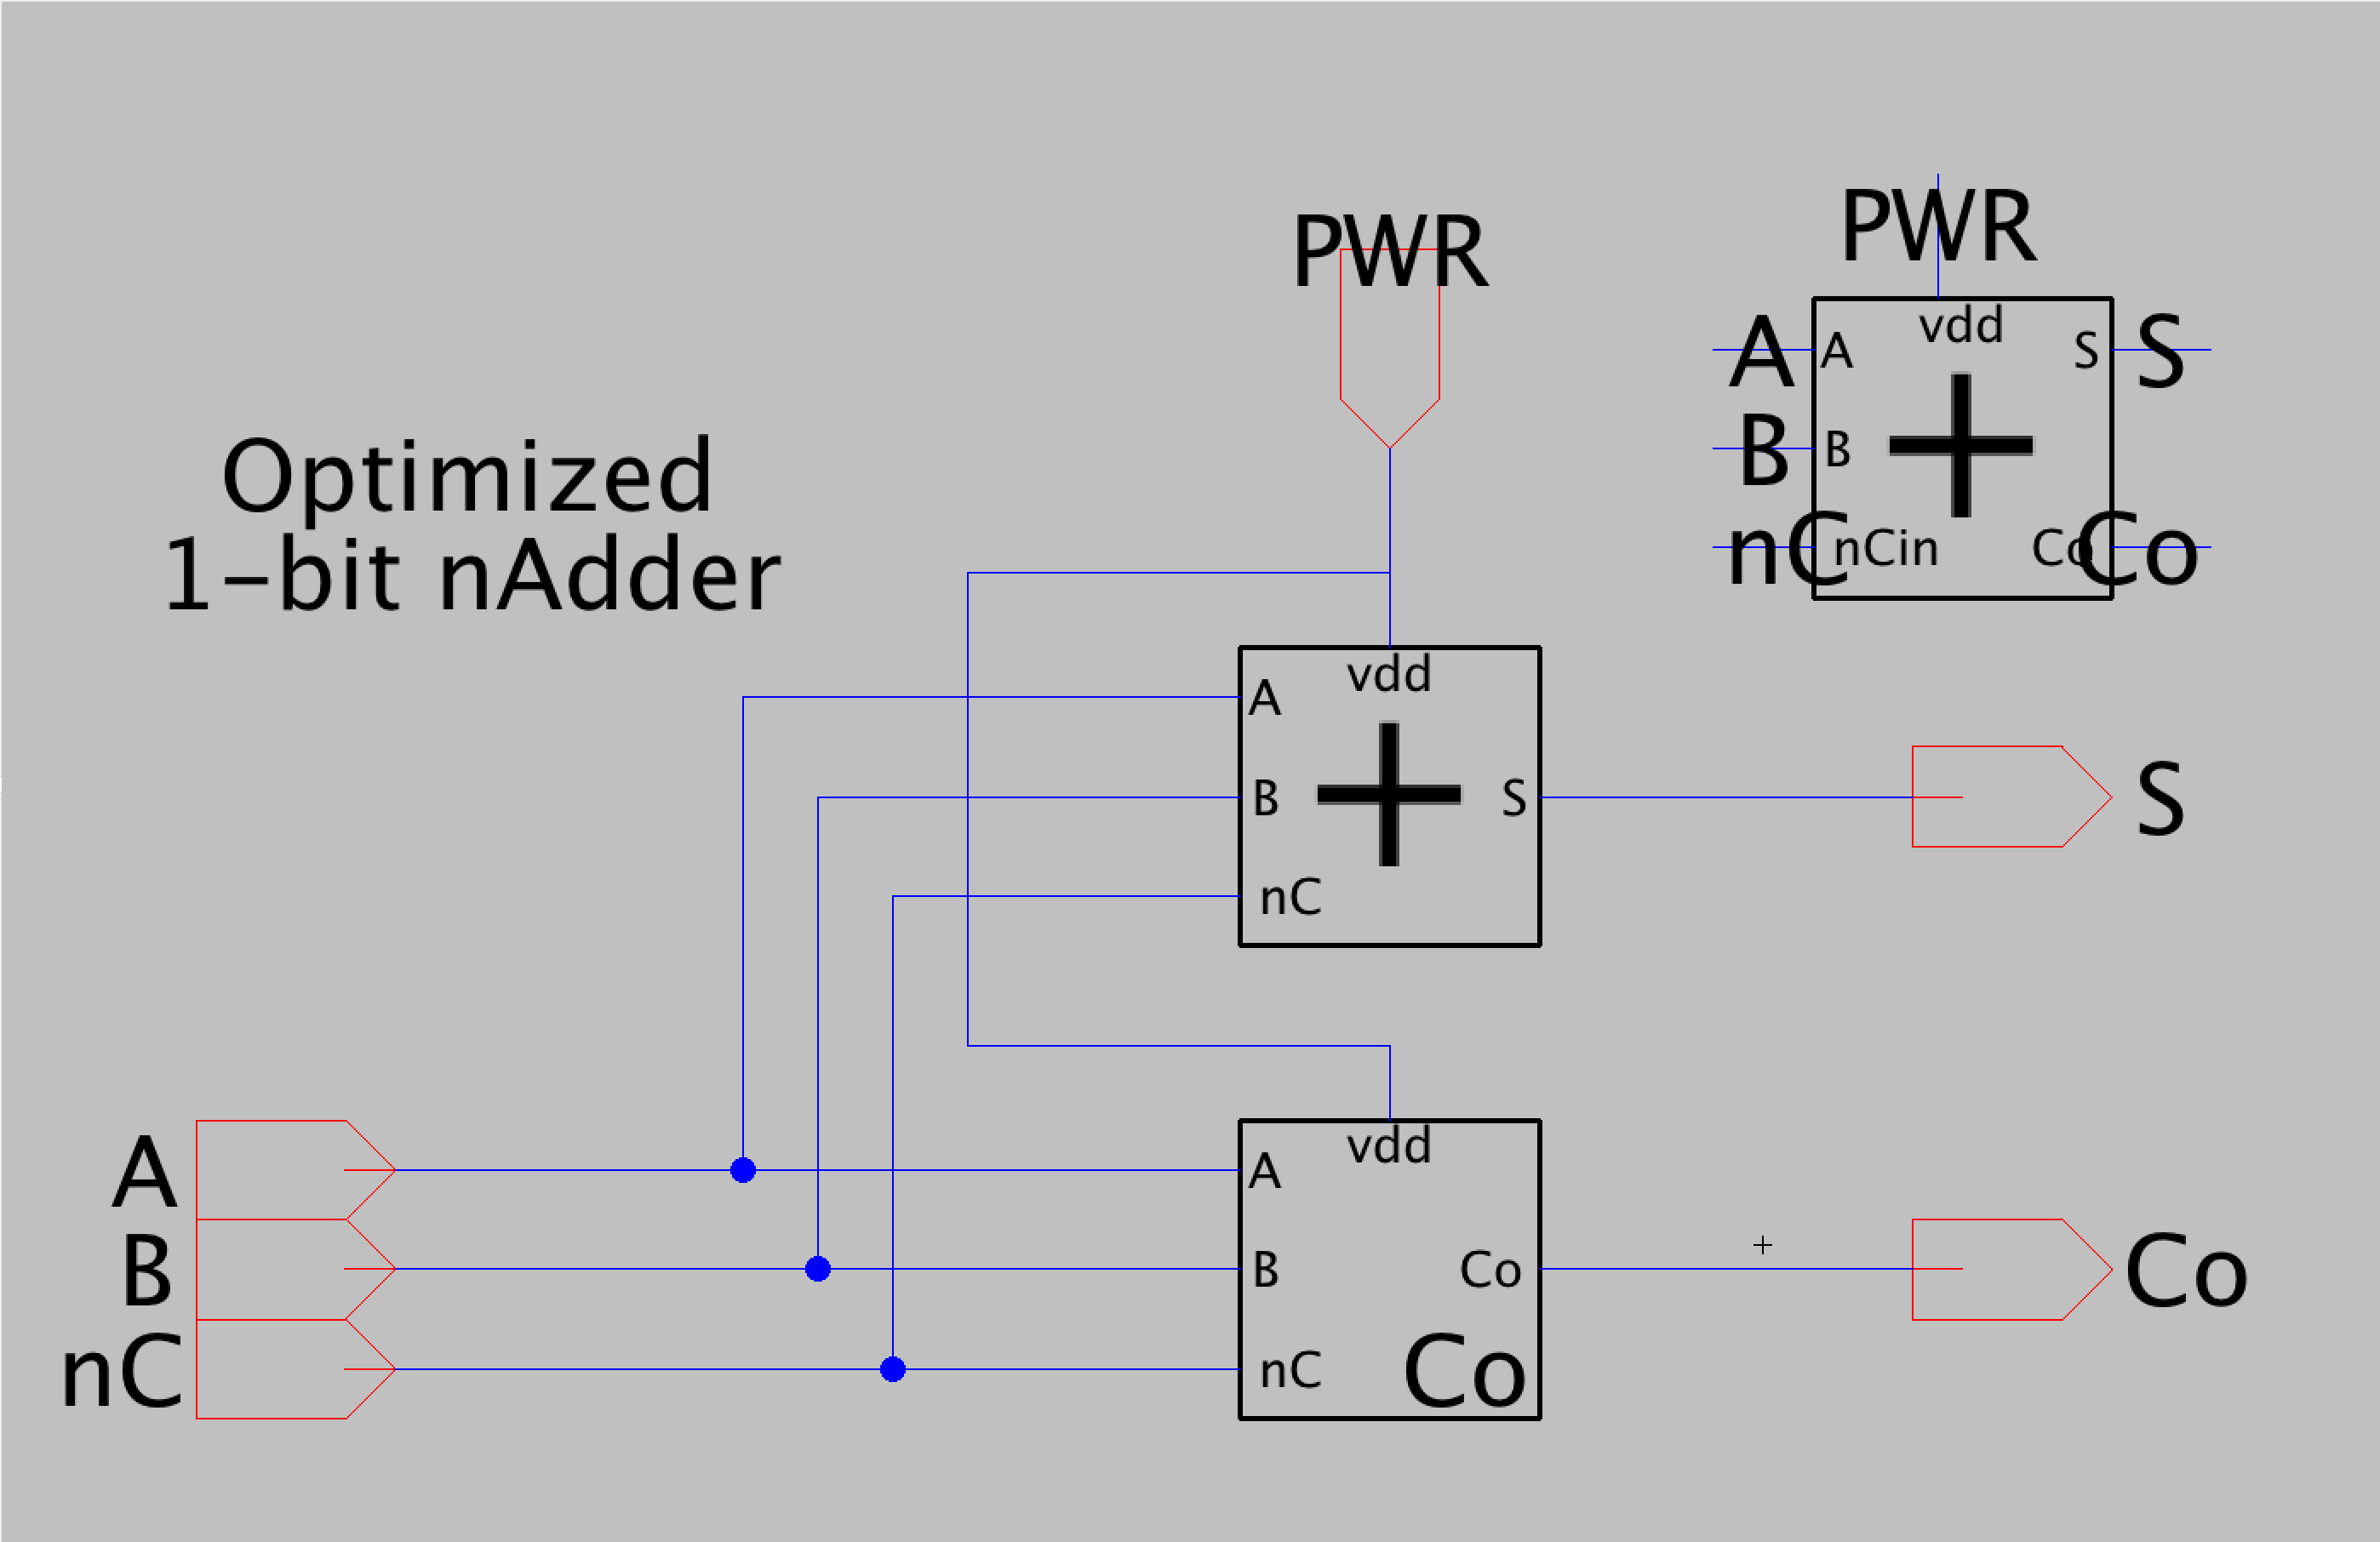
\includegraphics[width=\linewidth]{opt_screenshots/opt_1b_nadder_sch.png}
  \caption{Schematic for 1-b nAdder}
  \label{fig:opt_1b_nadder_sch}
\end{figure}

\begin{figure}[H]
  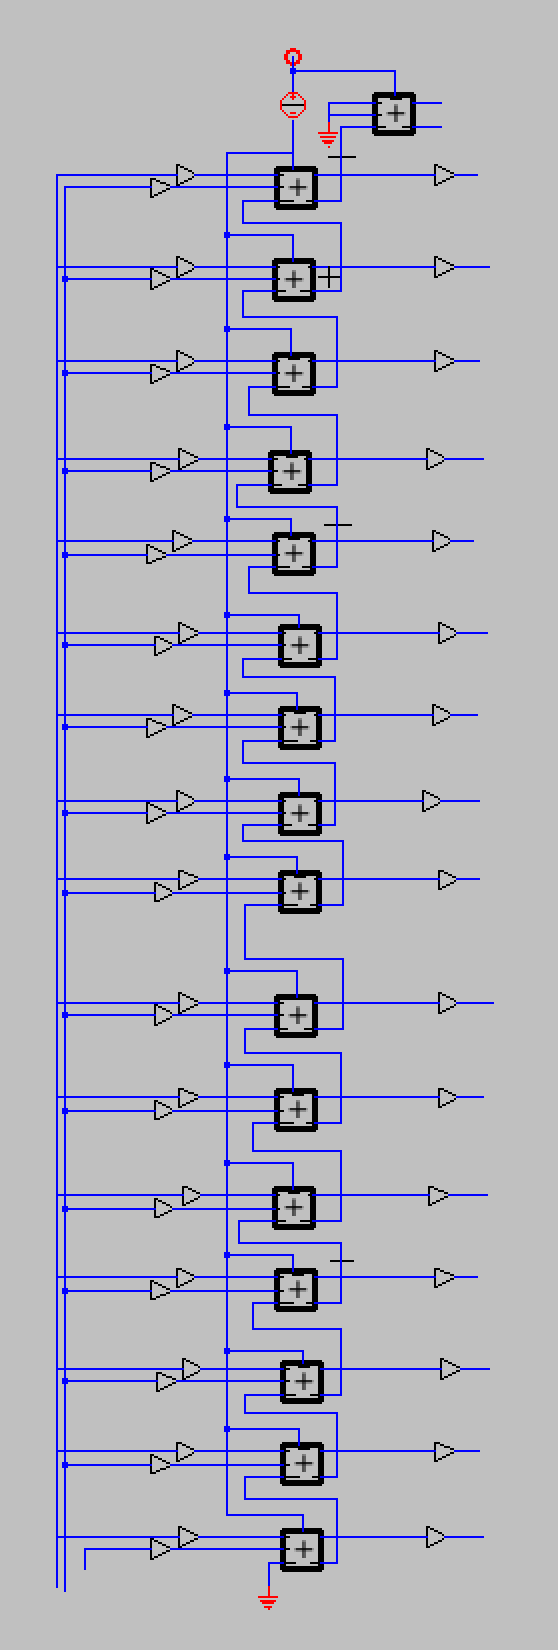
\includegraphics[width=\linewidth]{opt_screenshots/opt_16b_adder_sch.png}
  \caption{Schematic for entire 16-bit adder}
  \label{fig:opt_16b_adder_sch}
\end{figure}

\begin{figure}[H]
  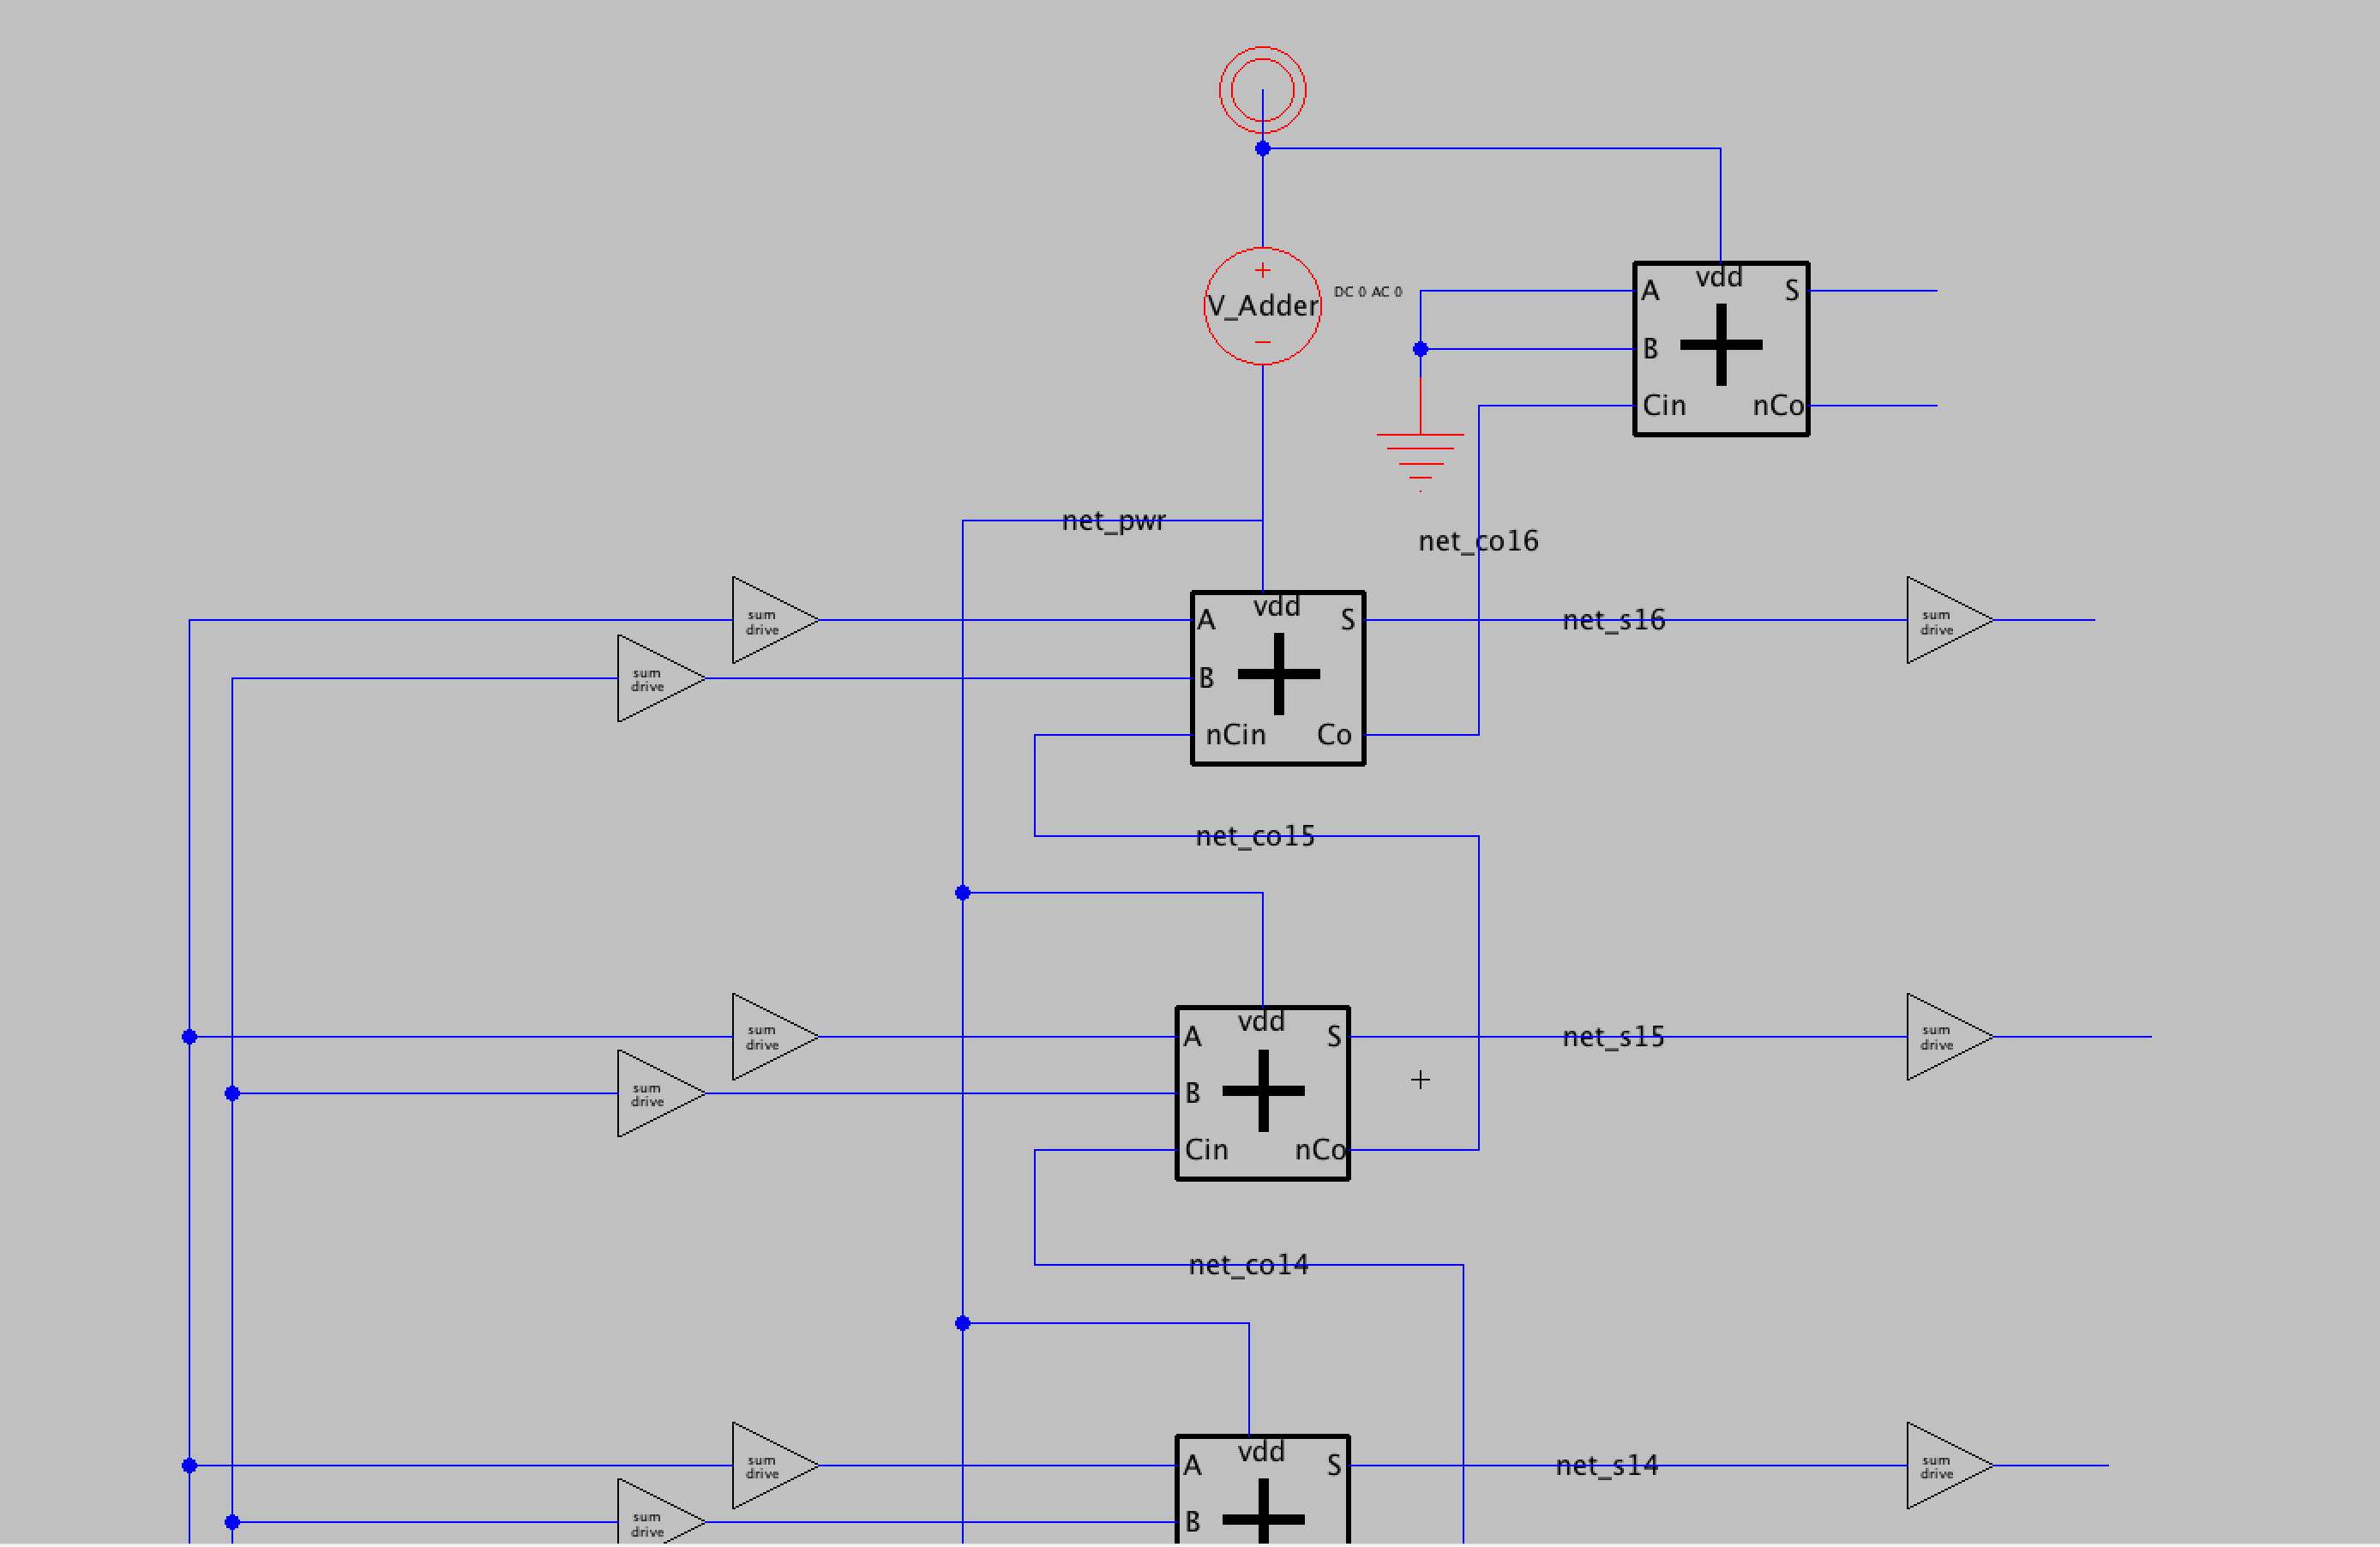
\includegraphics[width=\linewidth]{opt_screenshots/opt_16b_adder_sch_zoom1.png}
  \caption{Portion of schematic for entire 16-bit adder}
  \label{fig:opt_16b_adder_sch_zoom1}
\end{figure}

\begin{figure}[H]
  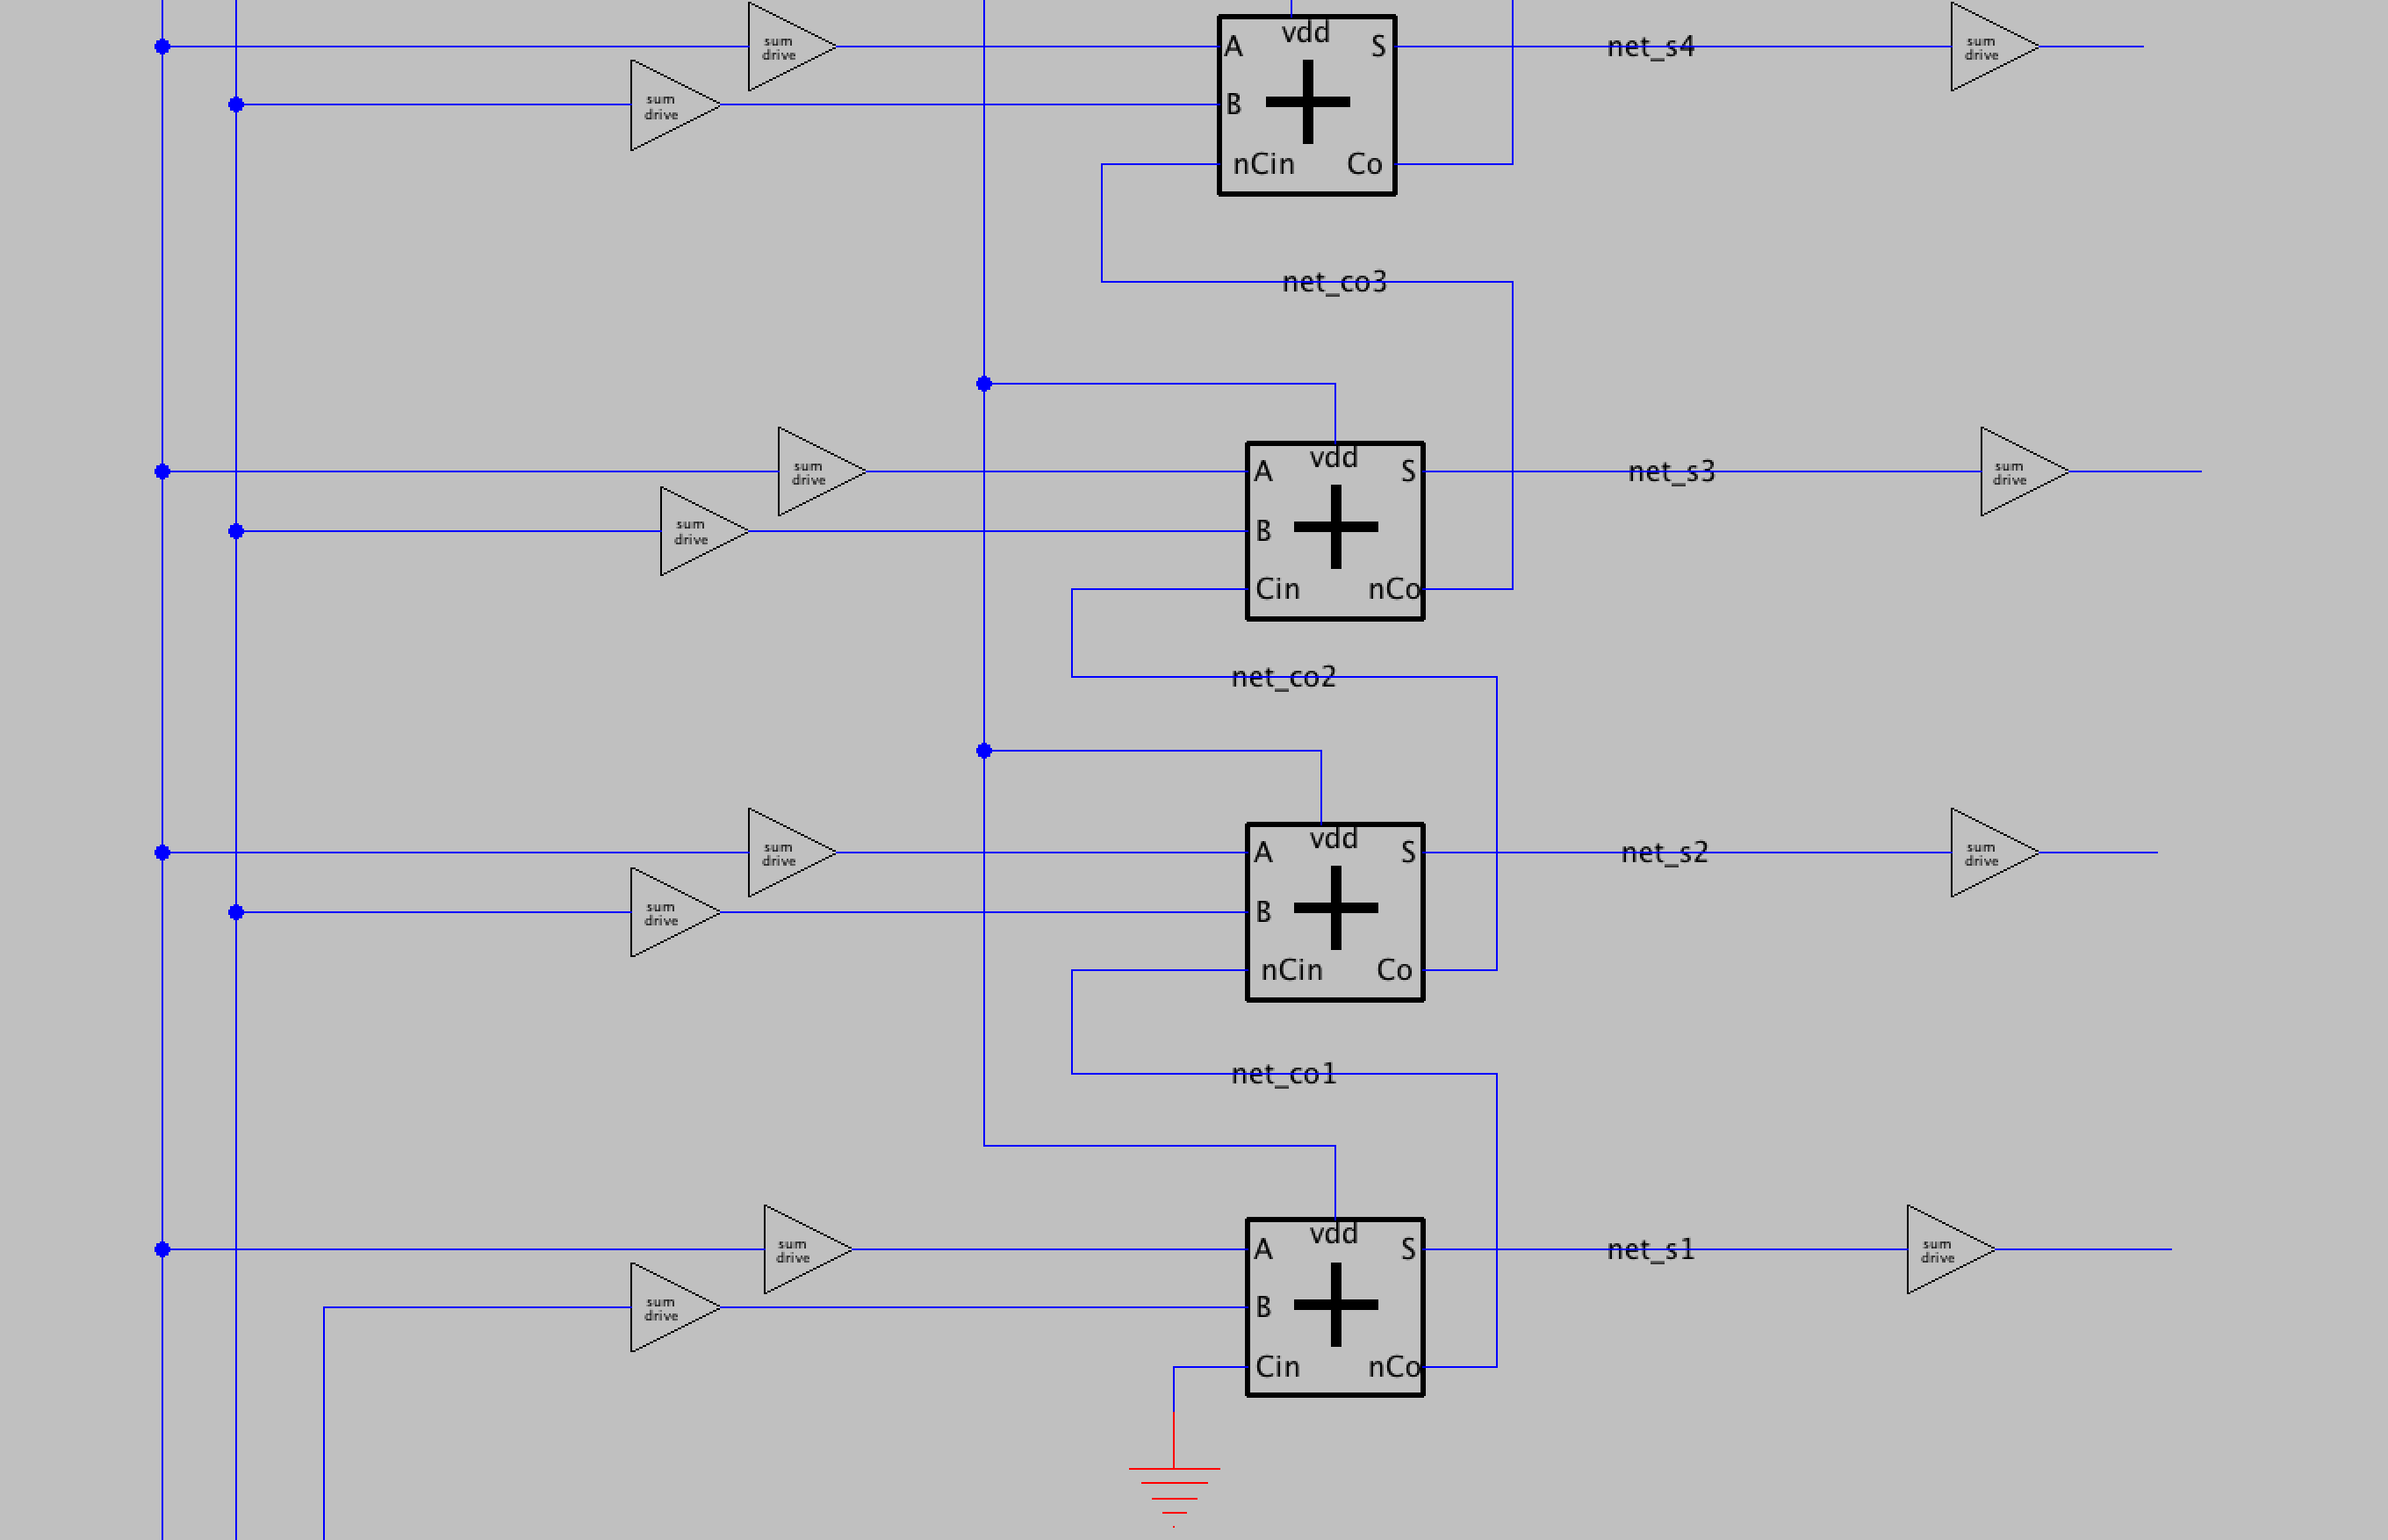
\includegraphics[width=\linewidth]{opt_screenshots/opt_16b_adder_sch_zoom2.png}
  \caption{Portion of schematic for entire 16-bit adder}
  \label{fig:opt_16b_adder_sch_zoom2}
\end{figure}


\section{Analysis of Optimized Design}
\subsection{Optimizing}
\subsubsection{The Optimization Process}
I went through a series of optimizations before arriving at the final design, checking the decrease in delay at each stage. Below is an enumeration of each optimization and the resulting measured delay across the entire adder.
\begin{enumerate}
\item Replace 3-input XOR with pass transistor logic XOR cascade ($667.123ps \rightarrow 528.022ps$)
\item Change $V_{dd} = 0.8V \rightarrow V_{dd} = 1V$ ($528.022ps \rightarrow 309.259ps$)
\item Re-order inputs to Carry and nCarry to reduce the $C_{diff}$ for the later input ($309.259ps \rightarrow 295.593ps$)
\item Increase width of transistors with $A$ and $B$ inputs for Carry and nCarry  ($295.593ps \rightarrow 274.925ps$)
\item Add step-up stages for $A$ and $B$ inputs for Carry and nCarry  ($274.925ps \rightarrow 280.286ps$)*
\item Add step-up stages for $A$ and $B$ inputs for 1-bit Adder  ($274.925ps \rightarrow 271.282ps$)
\item Add step-up stages for $A$ and $B$ inputs for 1-bit nAdder  ($271.282ps \rightarrow 271.864ps$)*
\end{enumerate}
Above are listed all the design optimizations that I considered, implemented, and ephemerally tested. Not all of these resulted in a decrease in delay (namely, the ones marked with *), and thus only the optimizations that decreased delay were used. Below are the schematics for the new XOR (Figure \ref{fig:pass_xor_sch}) and XNOR (Figure \ref{fig:pass_xnor_sch}) gates. Notice that these gates are NOT regenerative. I knew how I would be cascading them in such a way that the B input is never driven by another pass transistor, and the A input is restored by the gate. Furthermore, as you can see in Figure \ref{fig:opt_sum_sch} and Figure \ref{fig:opt_nsum_sch} above, the output of the final XOR or XNOR is regenerated by a final inverter. 

\begin{figure}[H]
  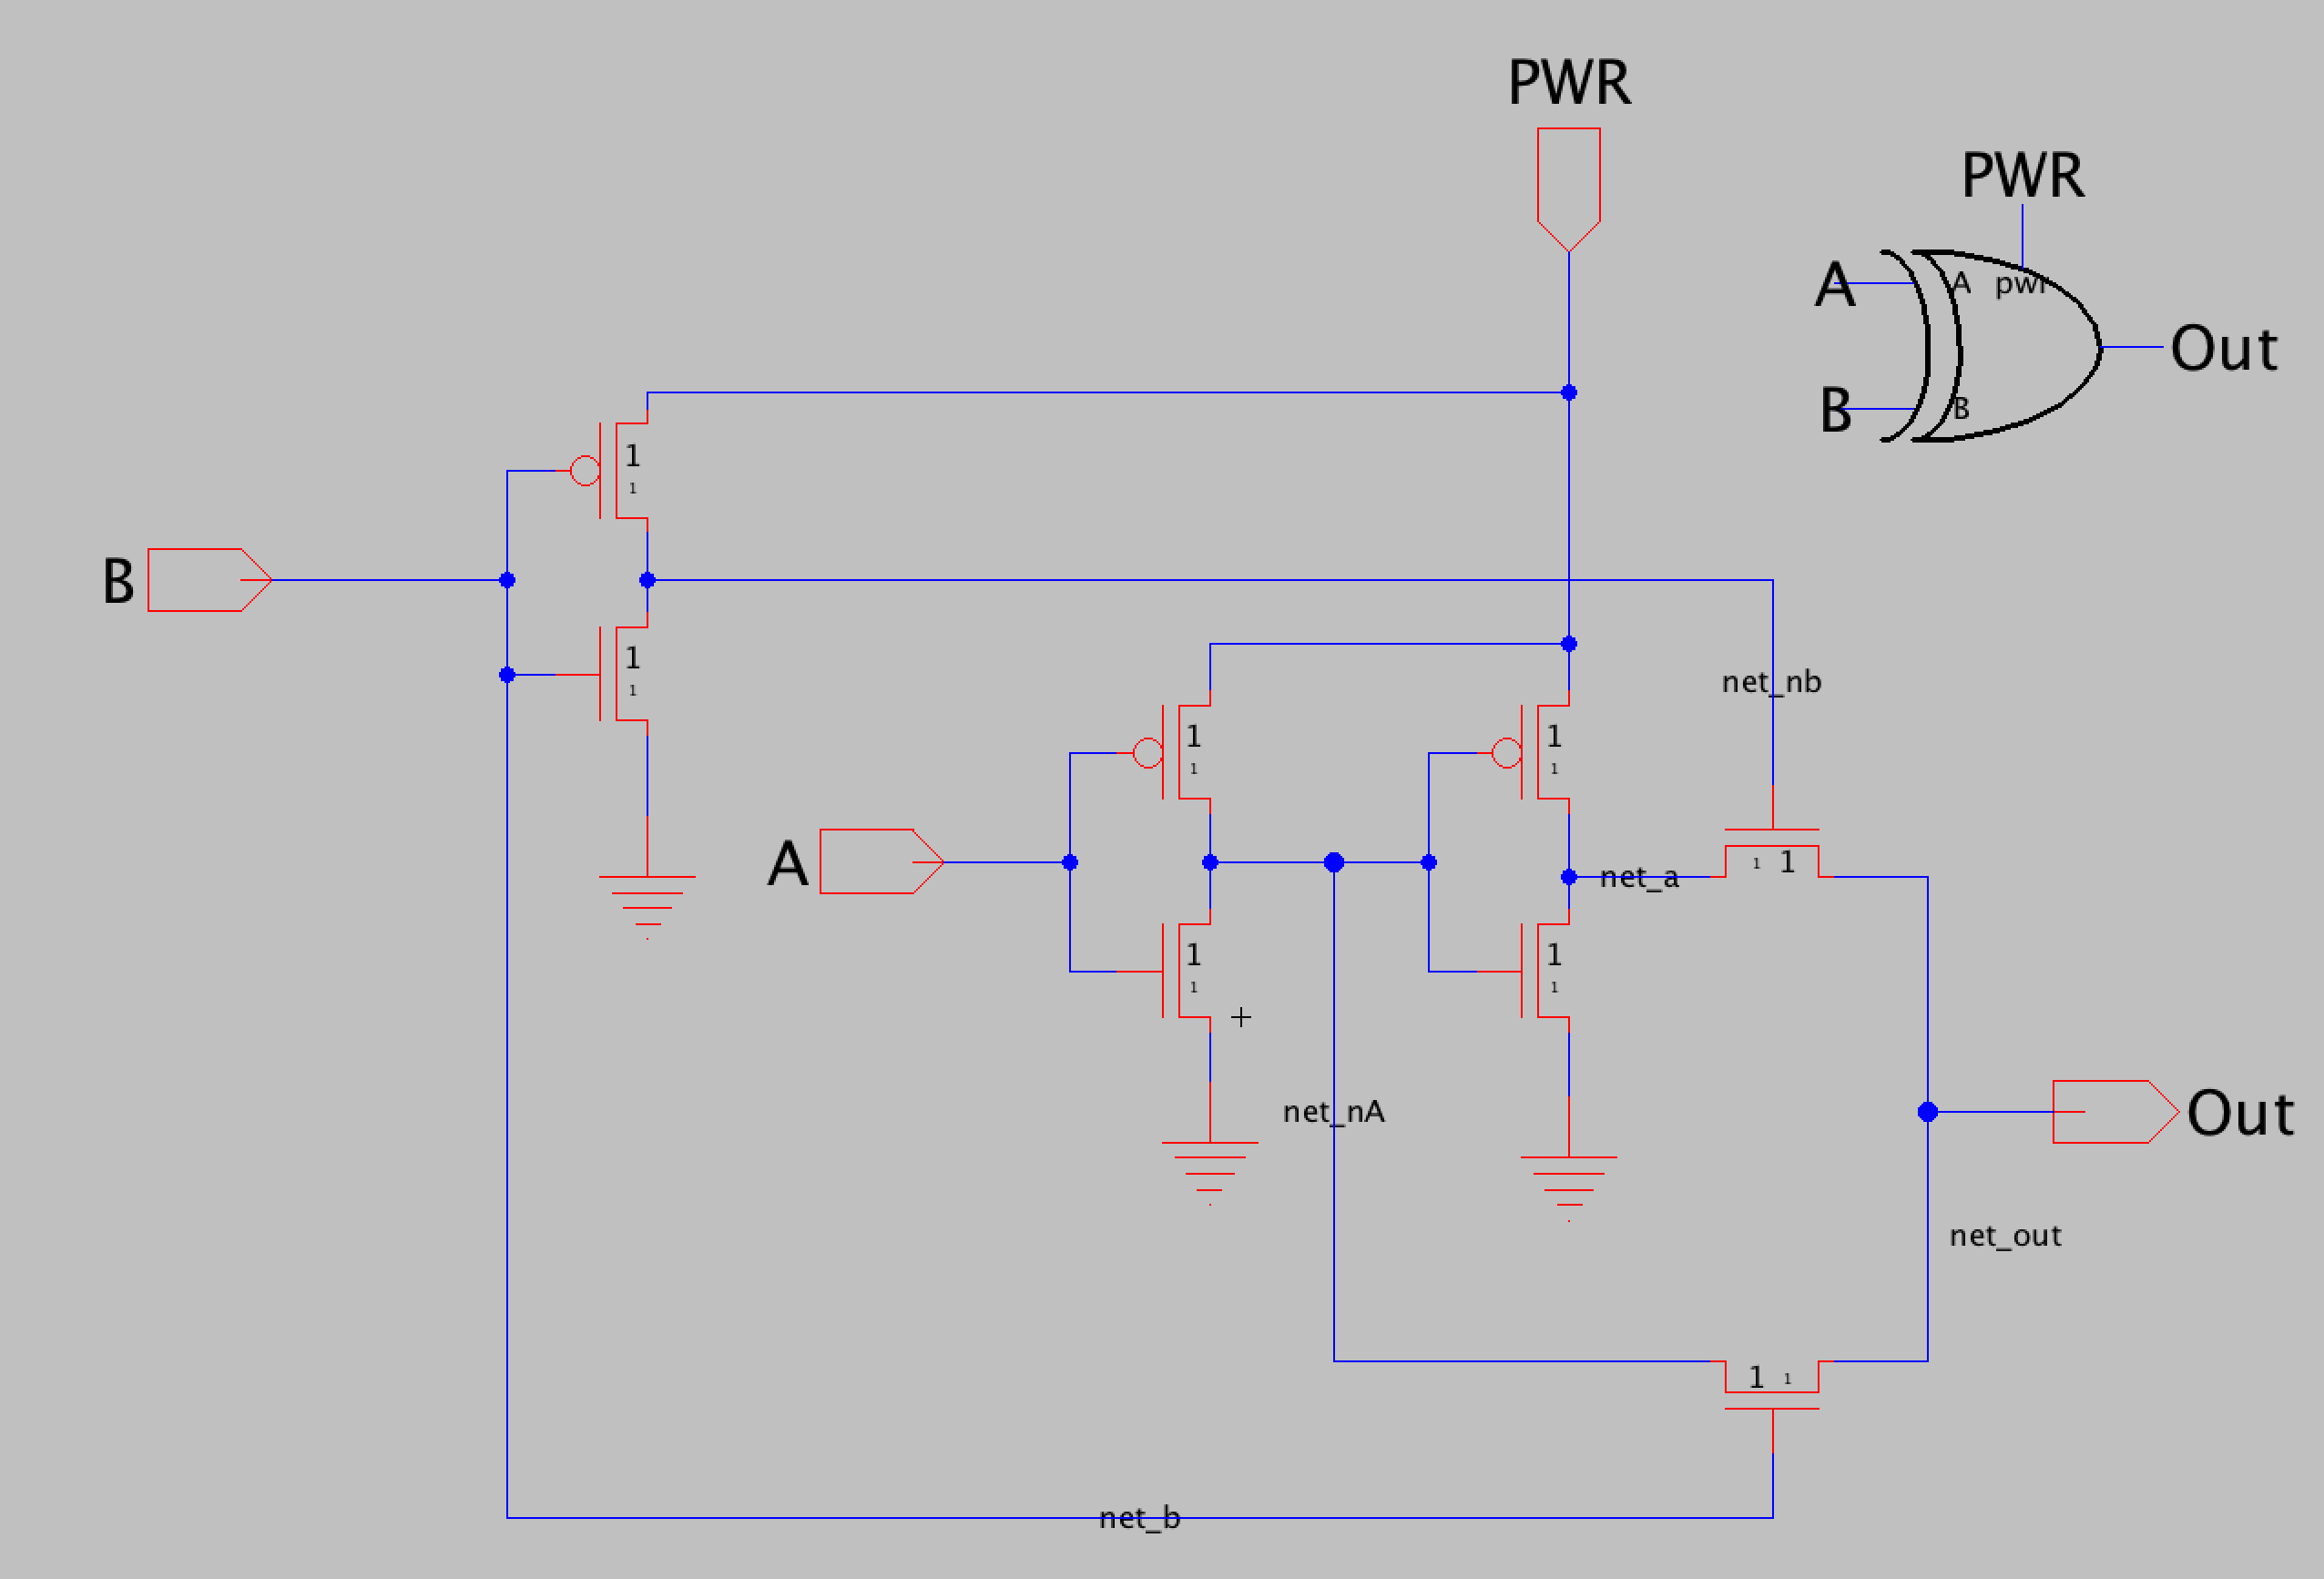
\includegraphics[width=\linewidth]{opt_screenshots/pass_xor_sch.png}
  \caption{Schematic for XOR with pass transistor logic}
  \label{fig:pass_xor_sch}
\end{figure}

\begin{figure}[H]
  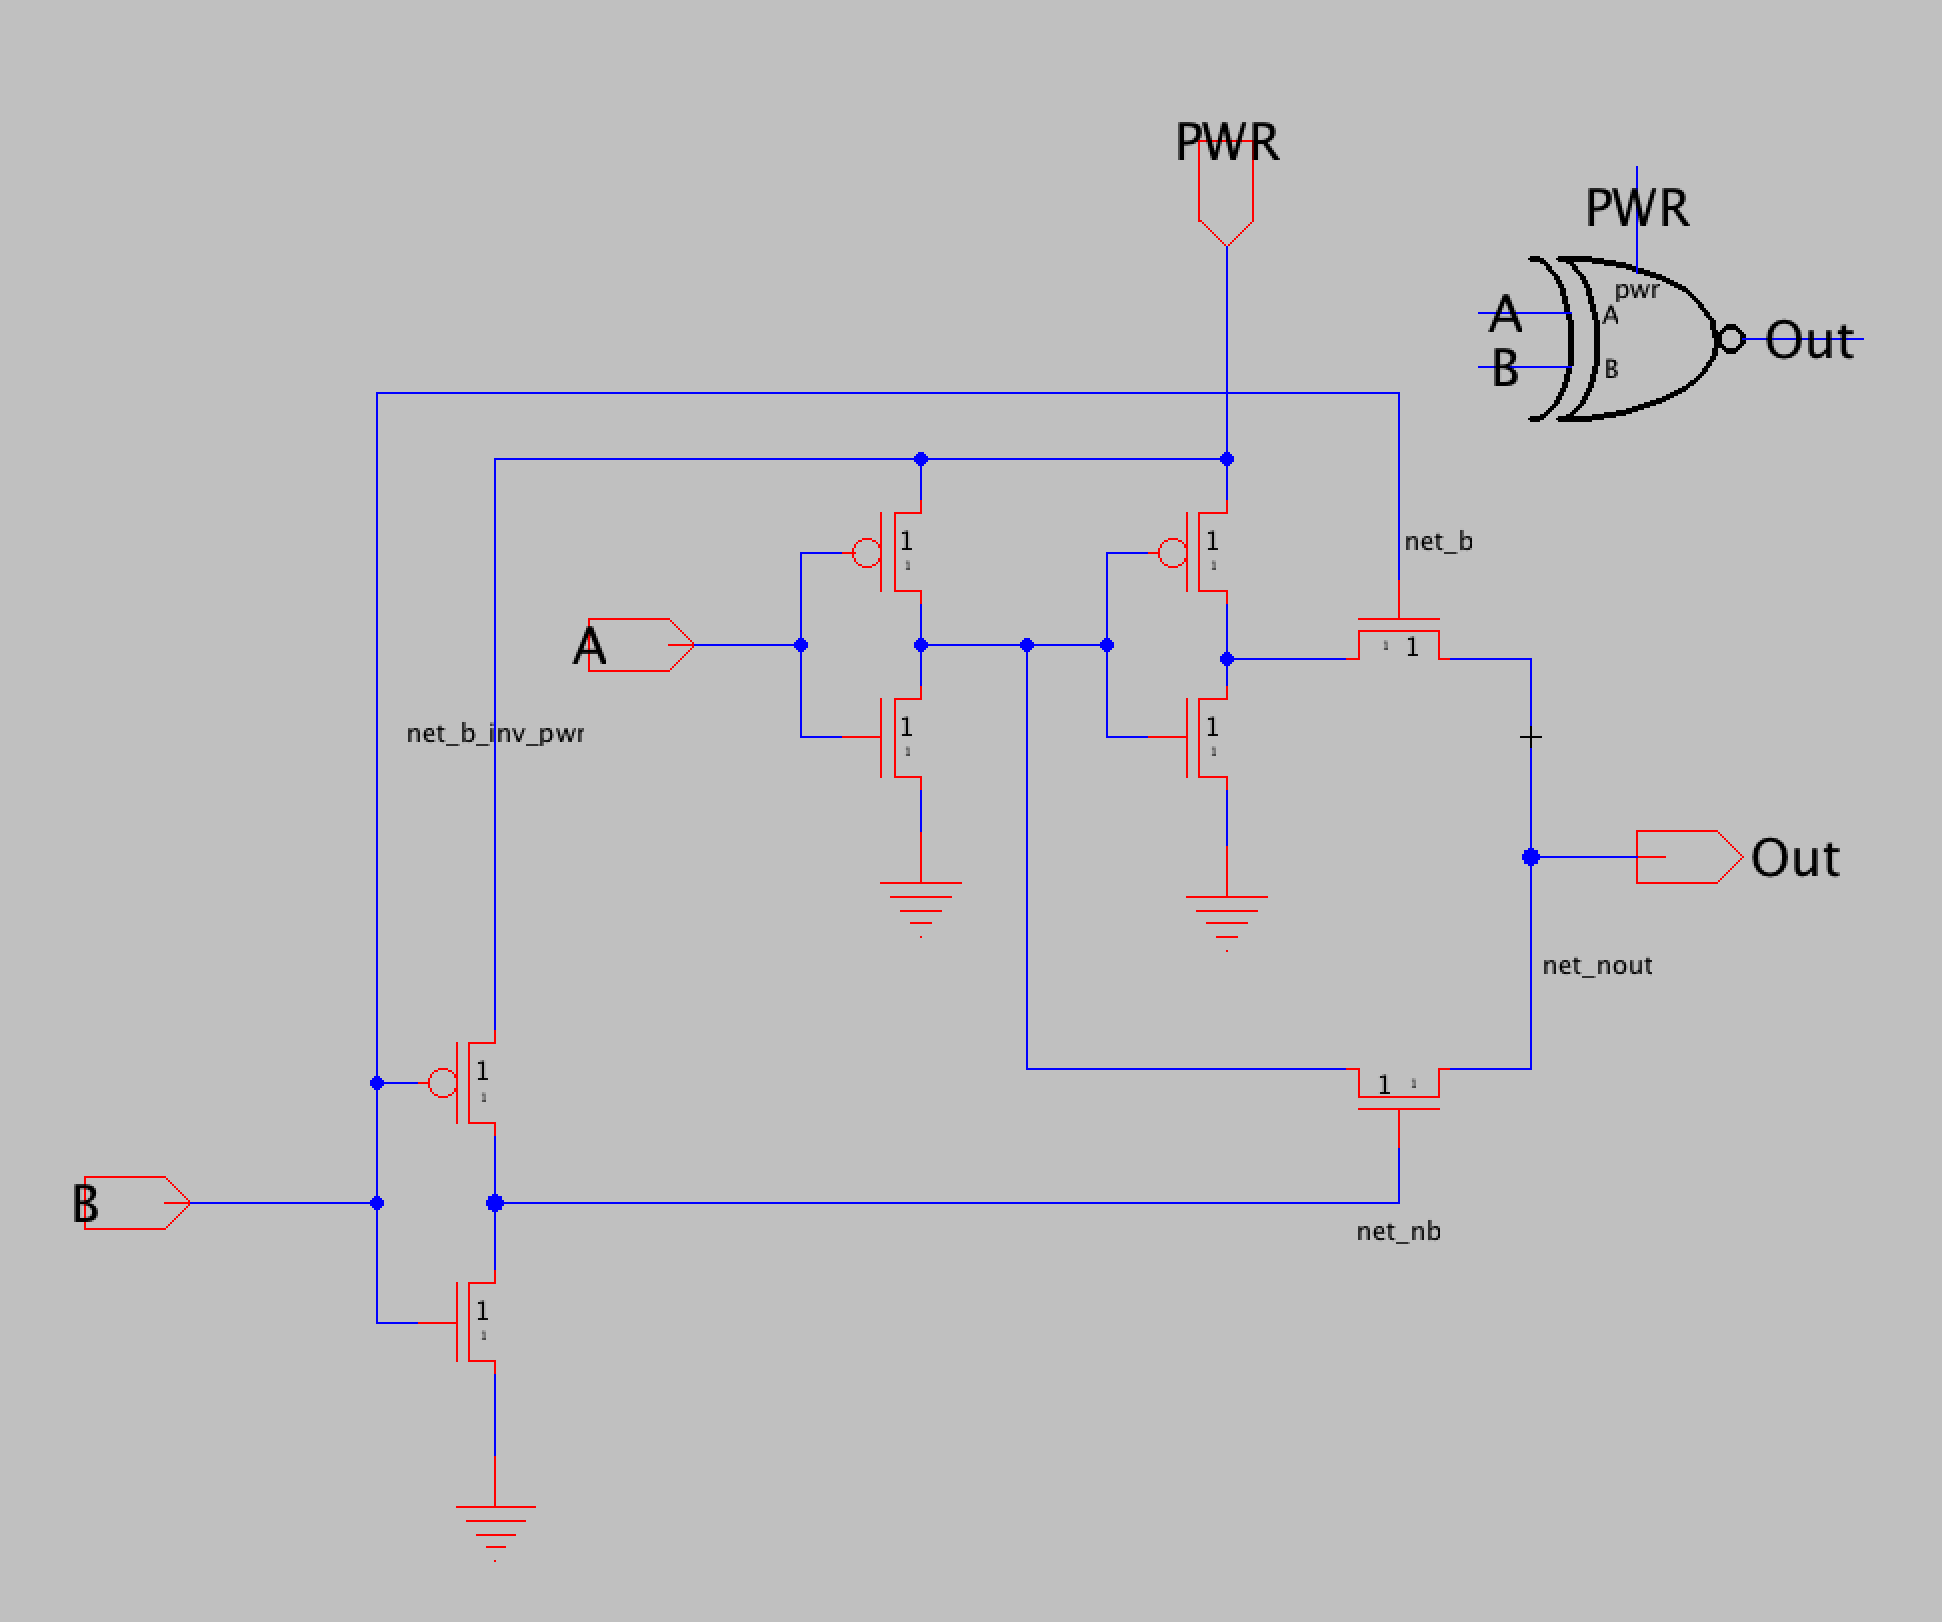
\includegraphics[width=\linewidth]{opt_screenshots/pass_xnor_sch.png}
  \caption{Schematic for XNOR with pass transistor logic}
  \label{fig:pass_xnor_sch}
\end{figure}

\subsection{Logical Correctness}
For all but the 16-bit adder, I checked every possible permutation of inputs. For the Sum, the output should be as shown in Figure \ref{fig:test_logic_ideal_sum_out}. For carry out, the target waveform is shown in Figure \ref{fig:test_logic_ideal_carry_out}.

\begin{figure}[H]
  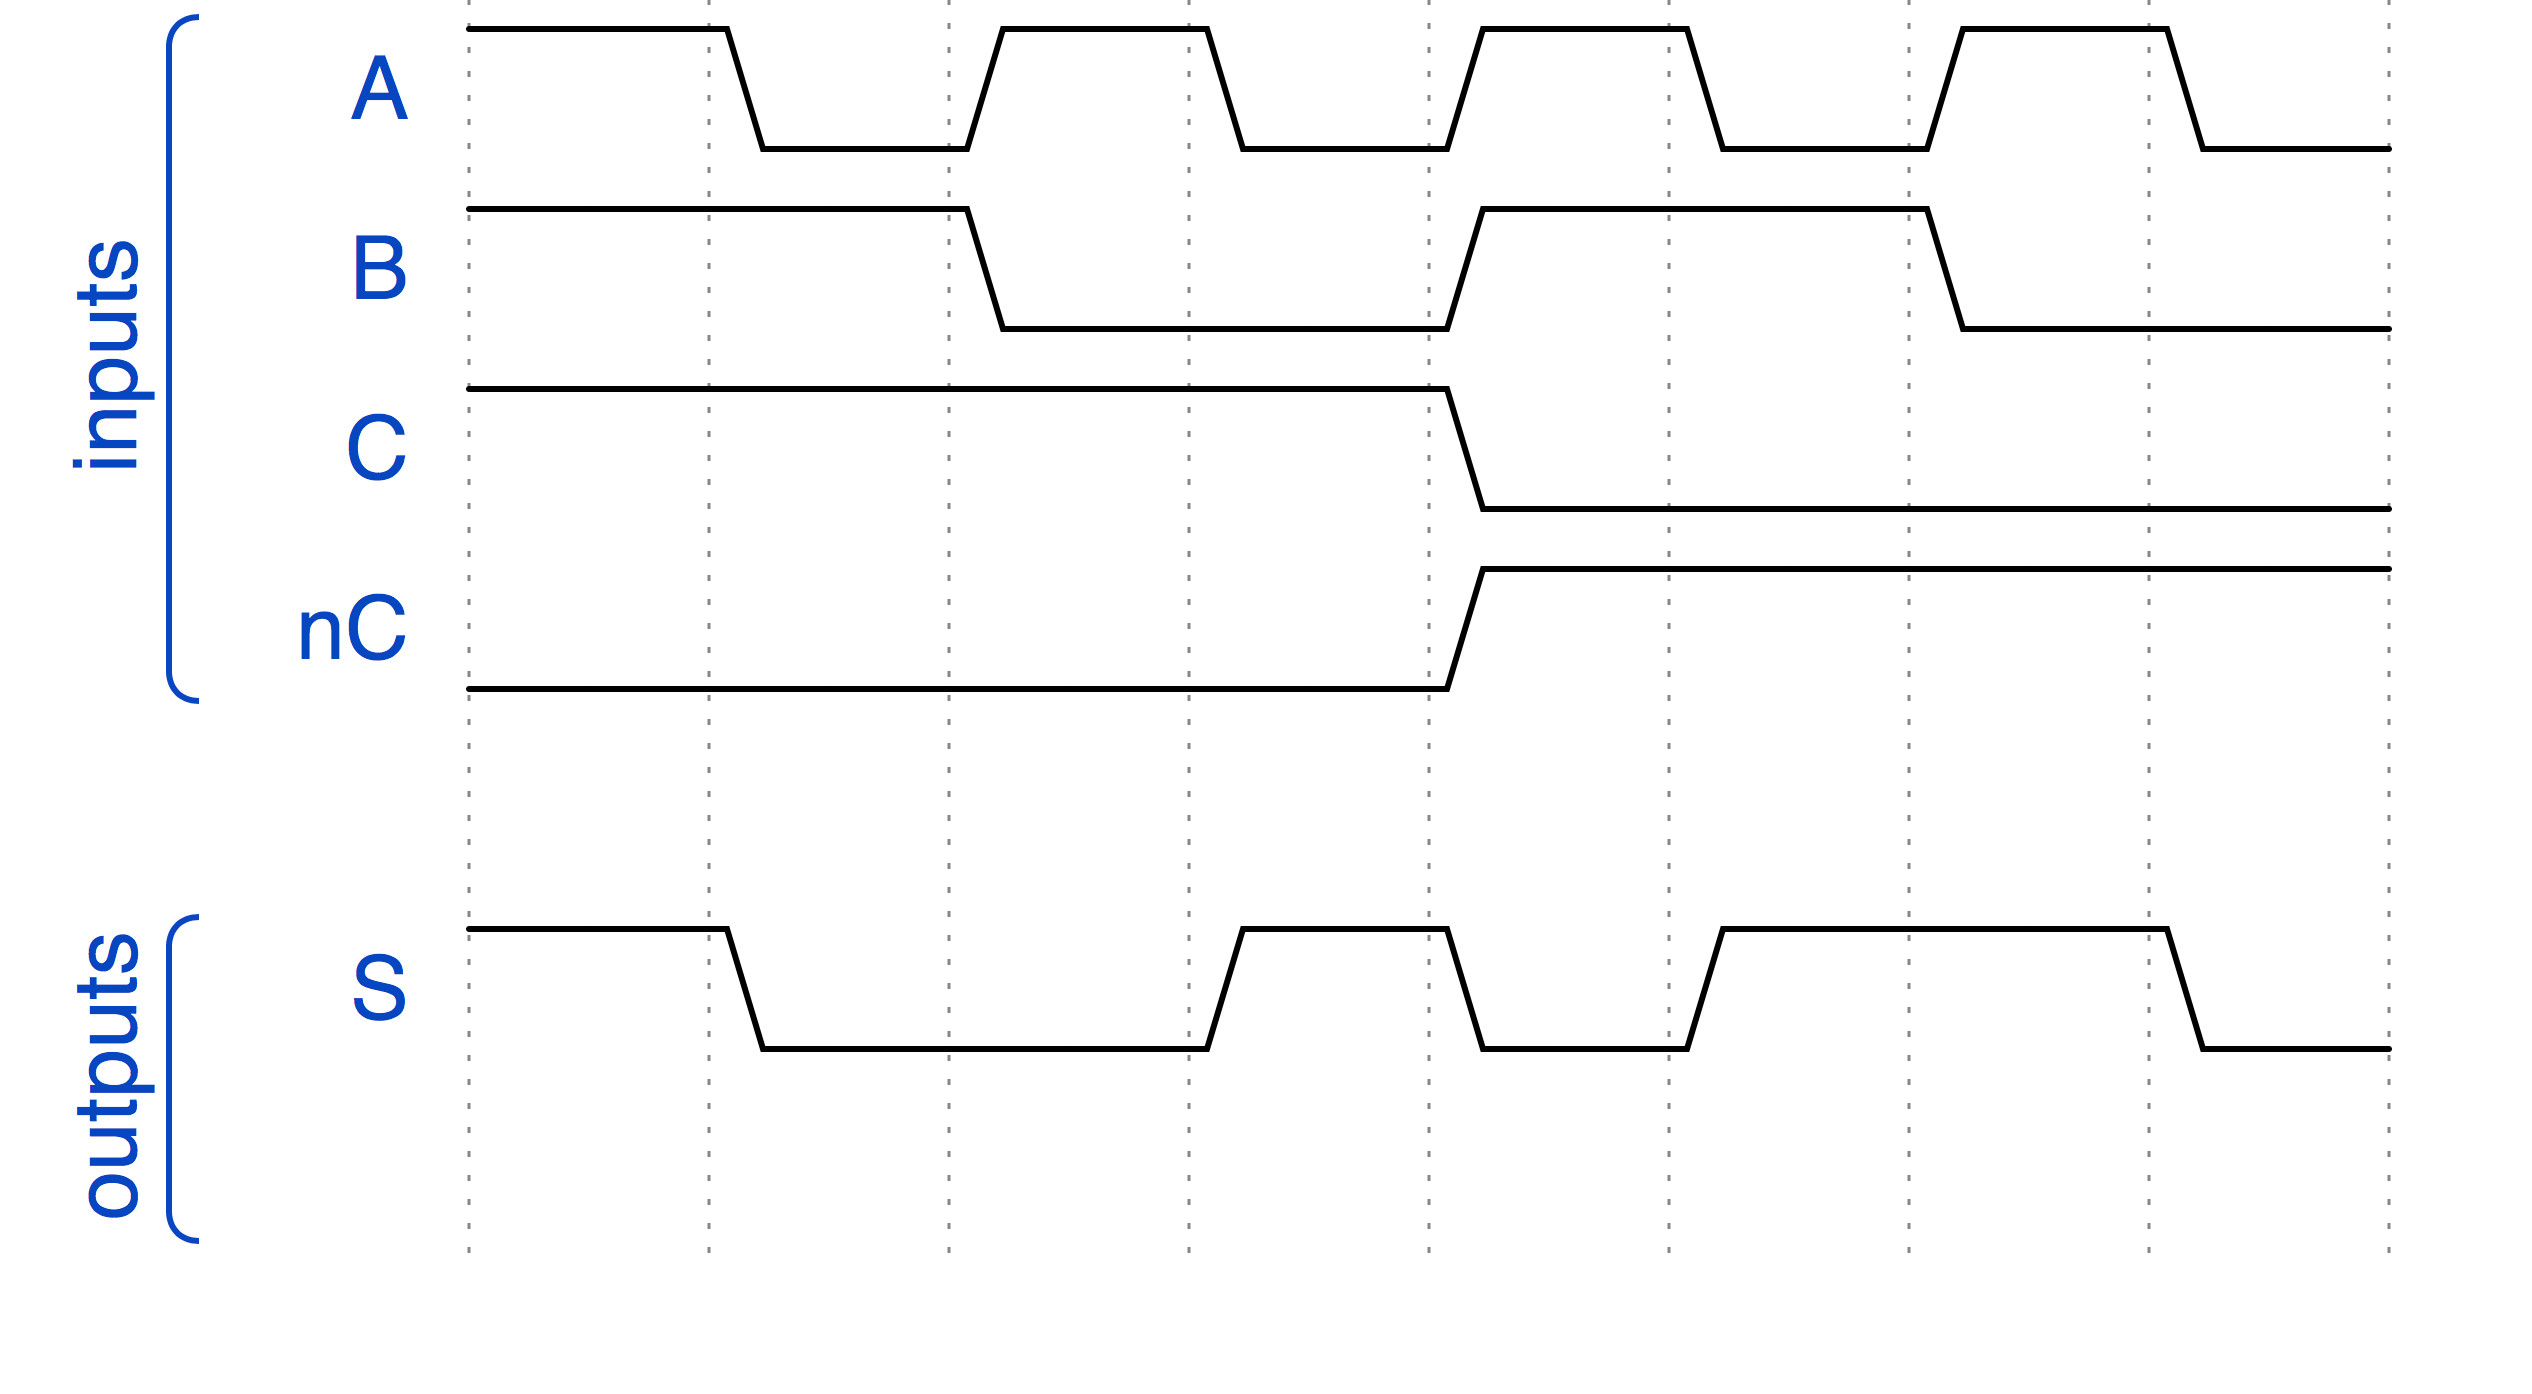
\includegraphics[width=\linewidth]{opt_screenshots/test_logic_ideal_sum_out.png}
  \caption{Target waveform for sum logic}
  \label{fig:test_logic_ideal_sum_out}
\end{figure}

\begin{figure}[H]
  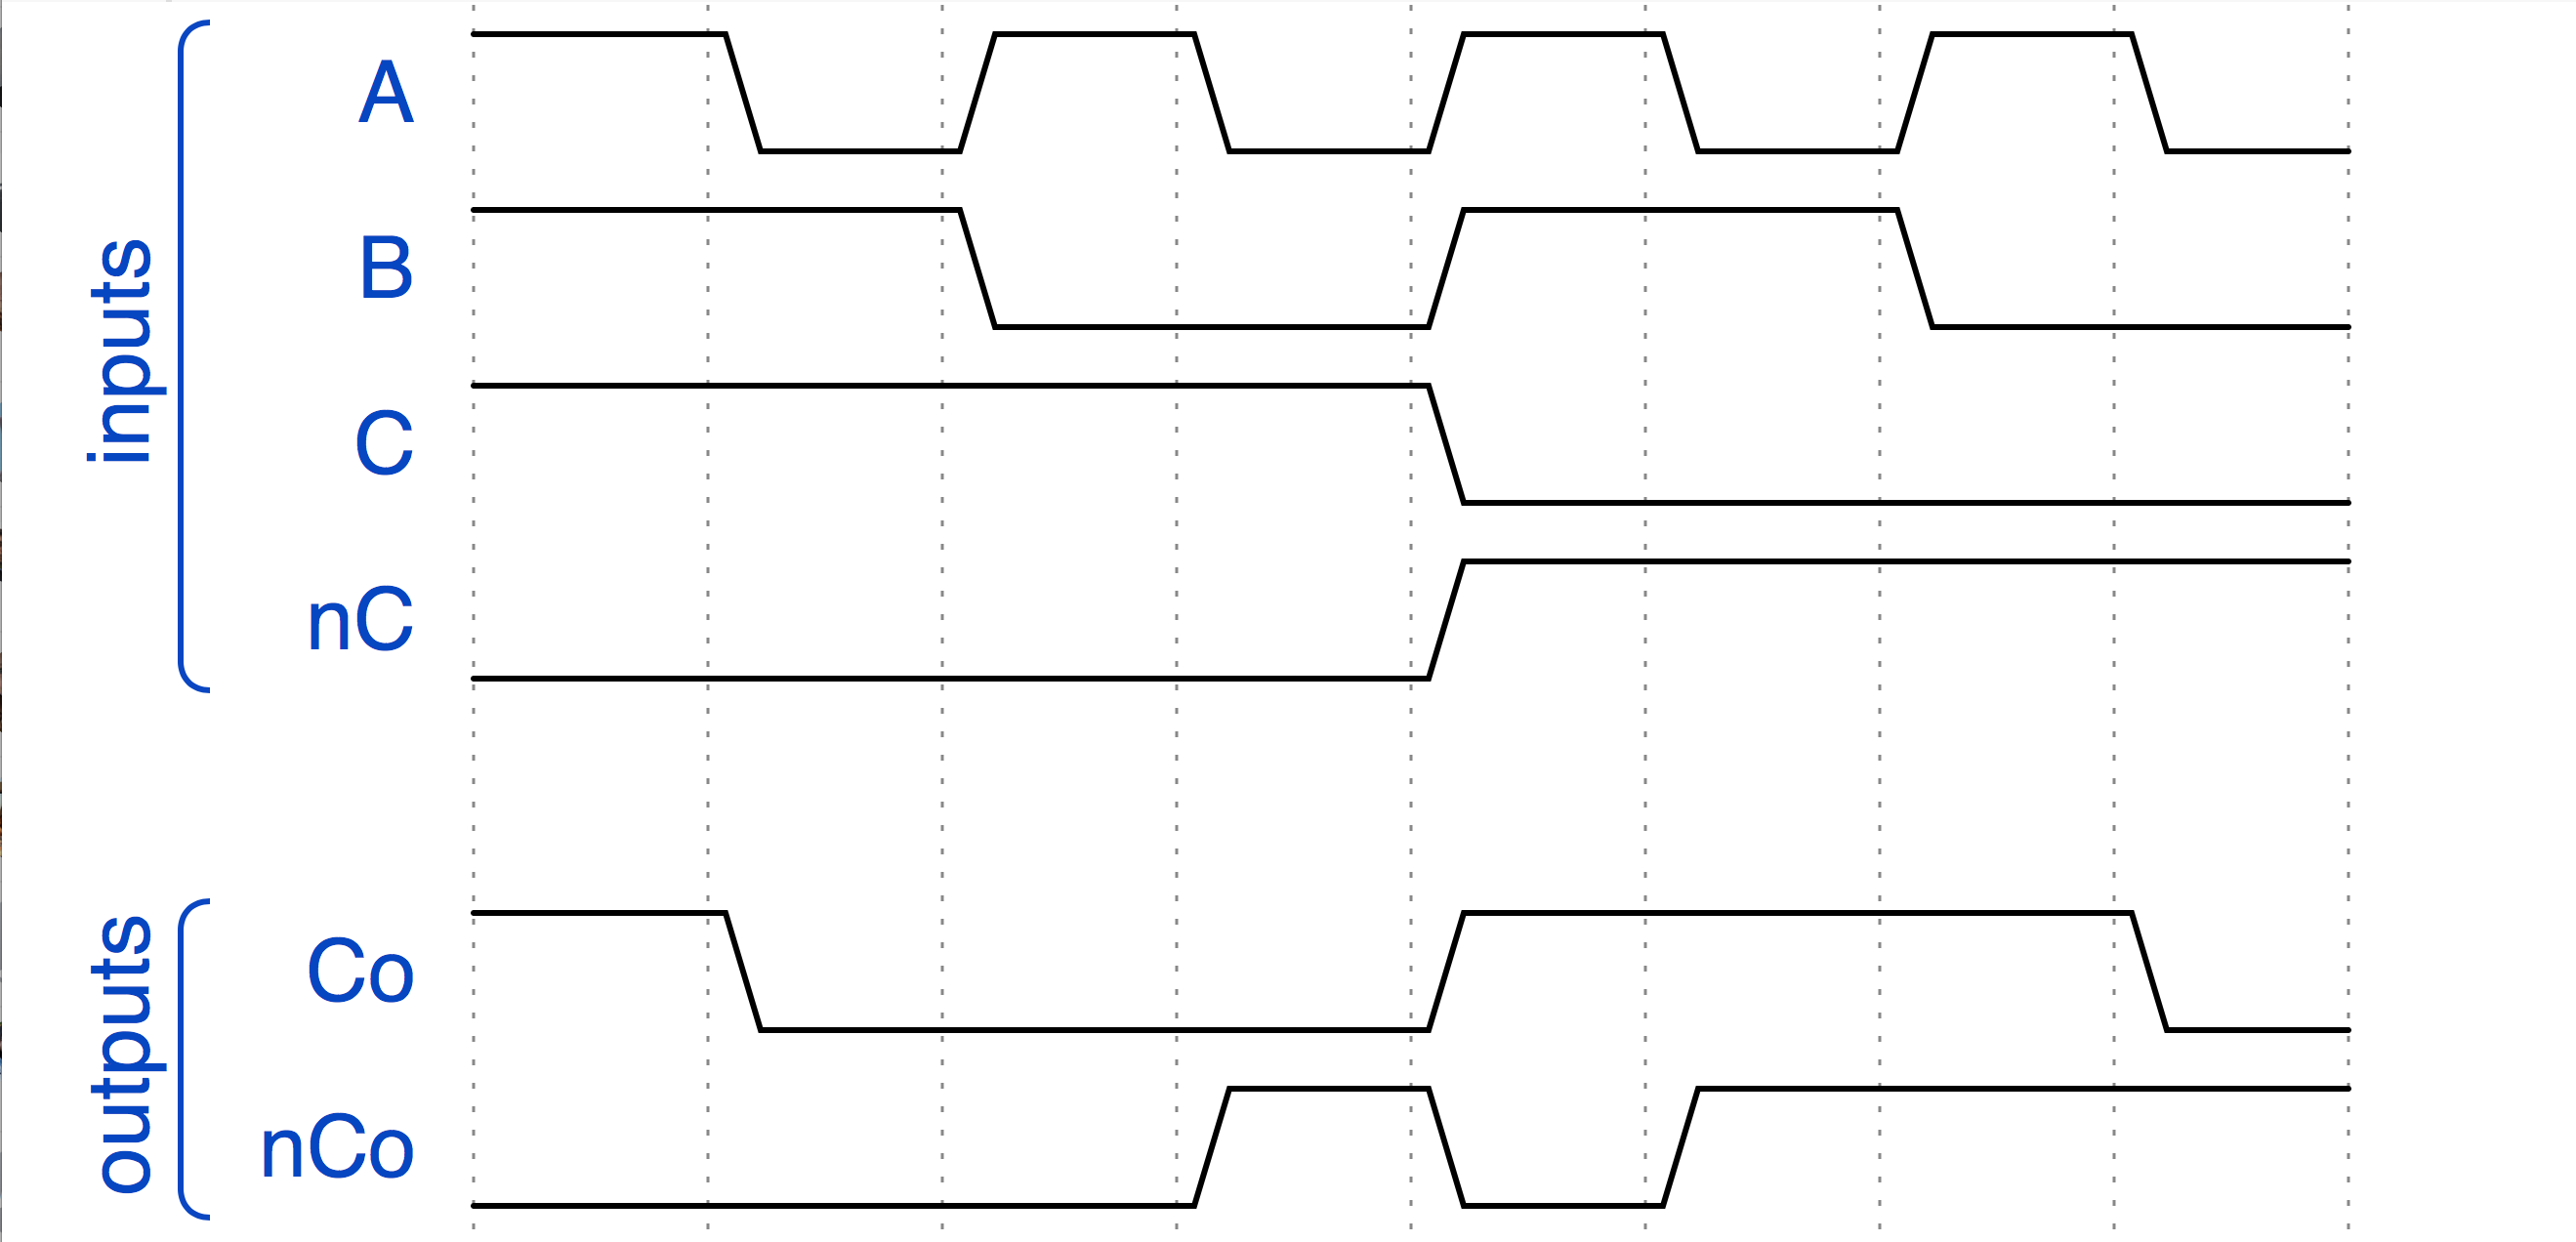
\includegraphics[width=\linewidth]{opt_screenshots/test_logic_ideal_carry_out.png}
  \caption{Target waveform for carry out logic}
  \label{fig:test_logic_ideal_carry_out}
\end{figure}

\subsubsection{Sum}
\begin{figure}[H]
  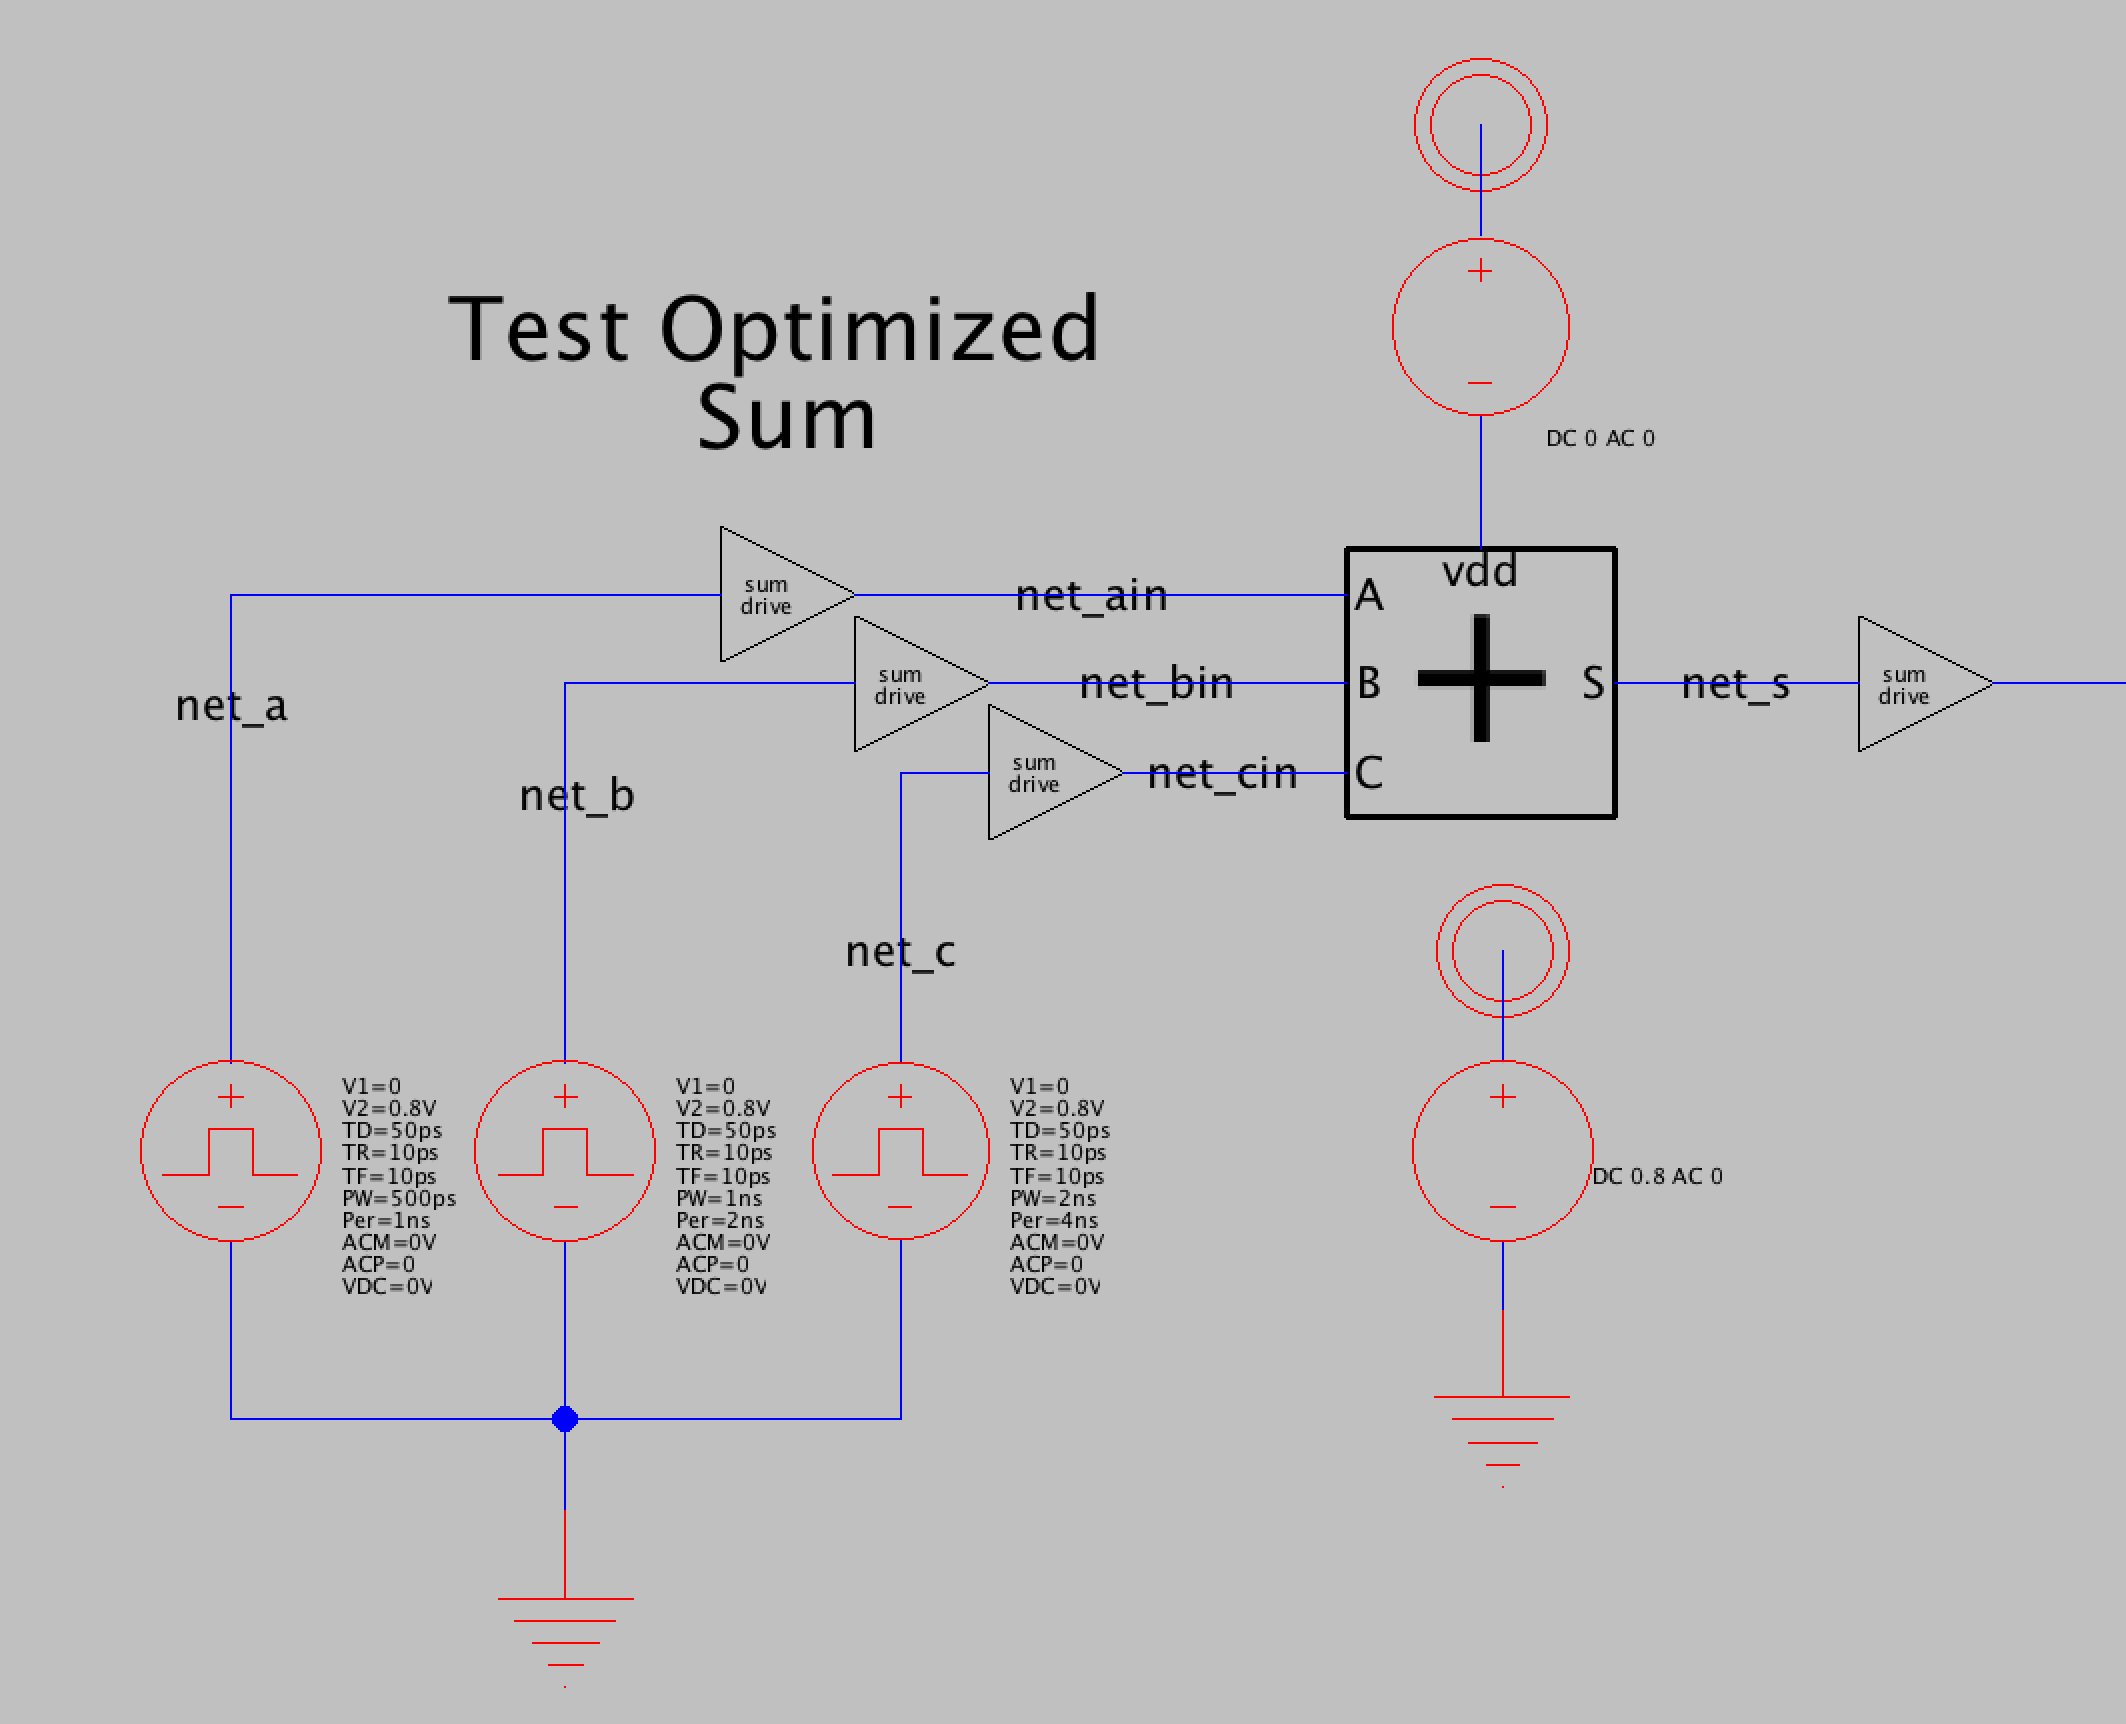
\includegraphics[width=\linewidth]{opt_screenshots/test_logic_sum_out_sch.png}
  \caption{Schematic used to test logical correctness of Sum}
  \label{fig:test_logic_sum_out_sch}
\end{figure}

\begin{figure}[H]
  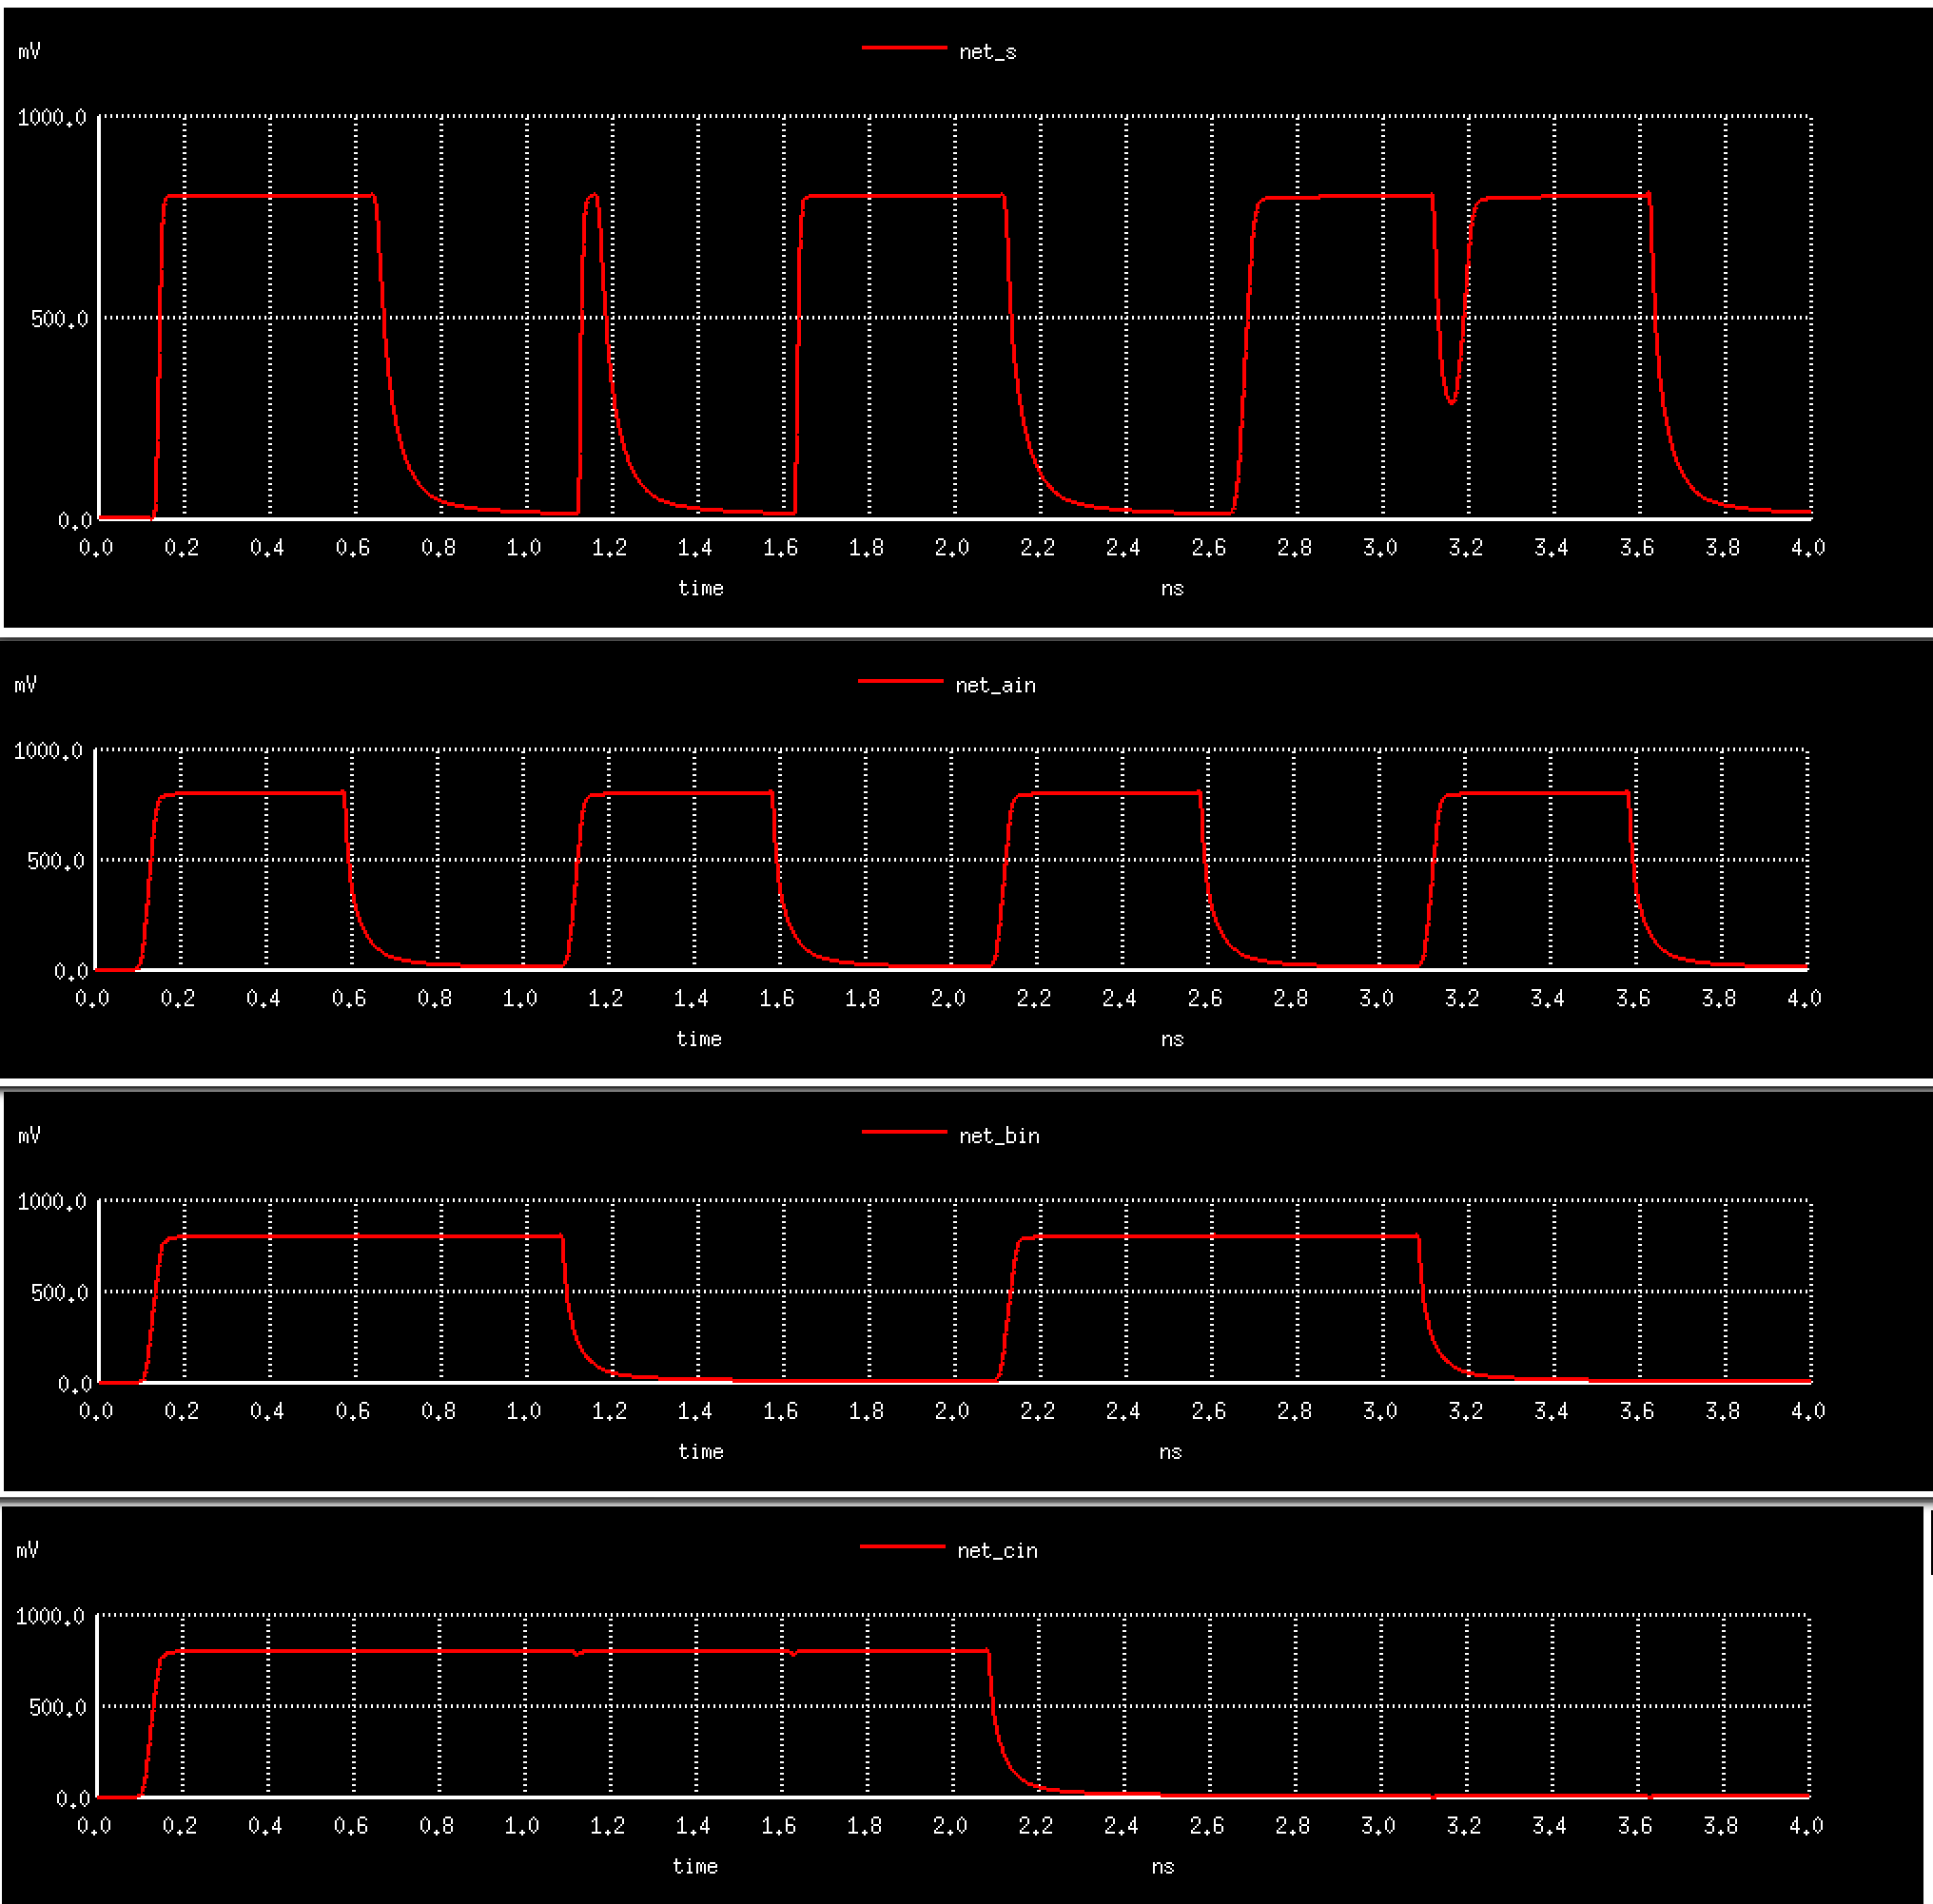
\includegraphics[width=\linewidth]{opt_screenshots/test_logic_sum_out.png}
  \caption{Waveform showing logical correctness of Sum}
  \label{fig:test_logic_sum_out}
\end{figure}

\subsubsection{nSum}
\begin{figure}[H]
  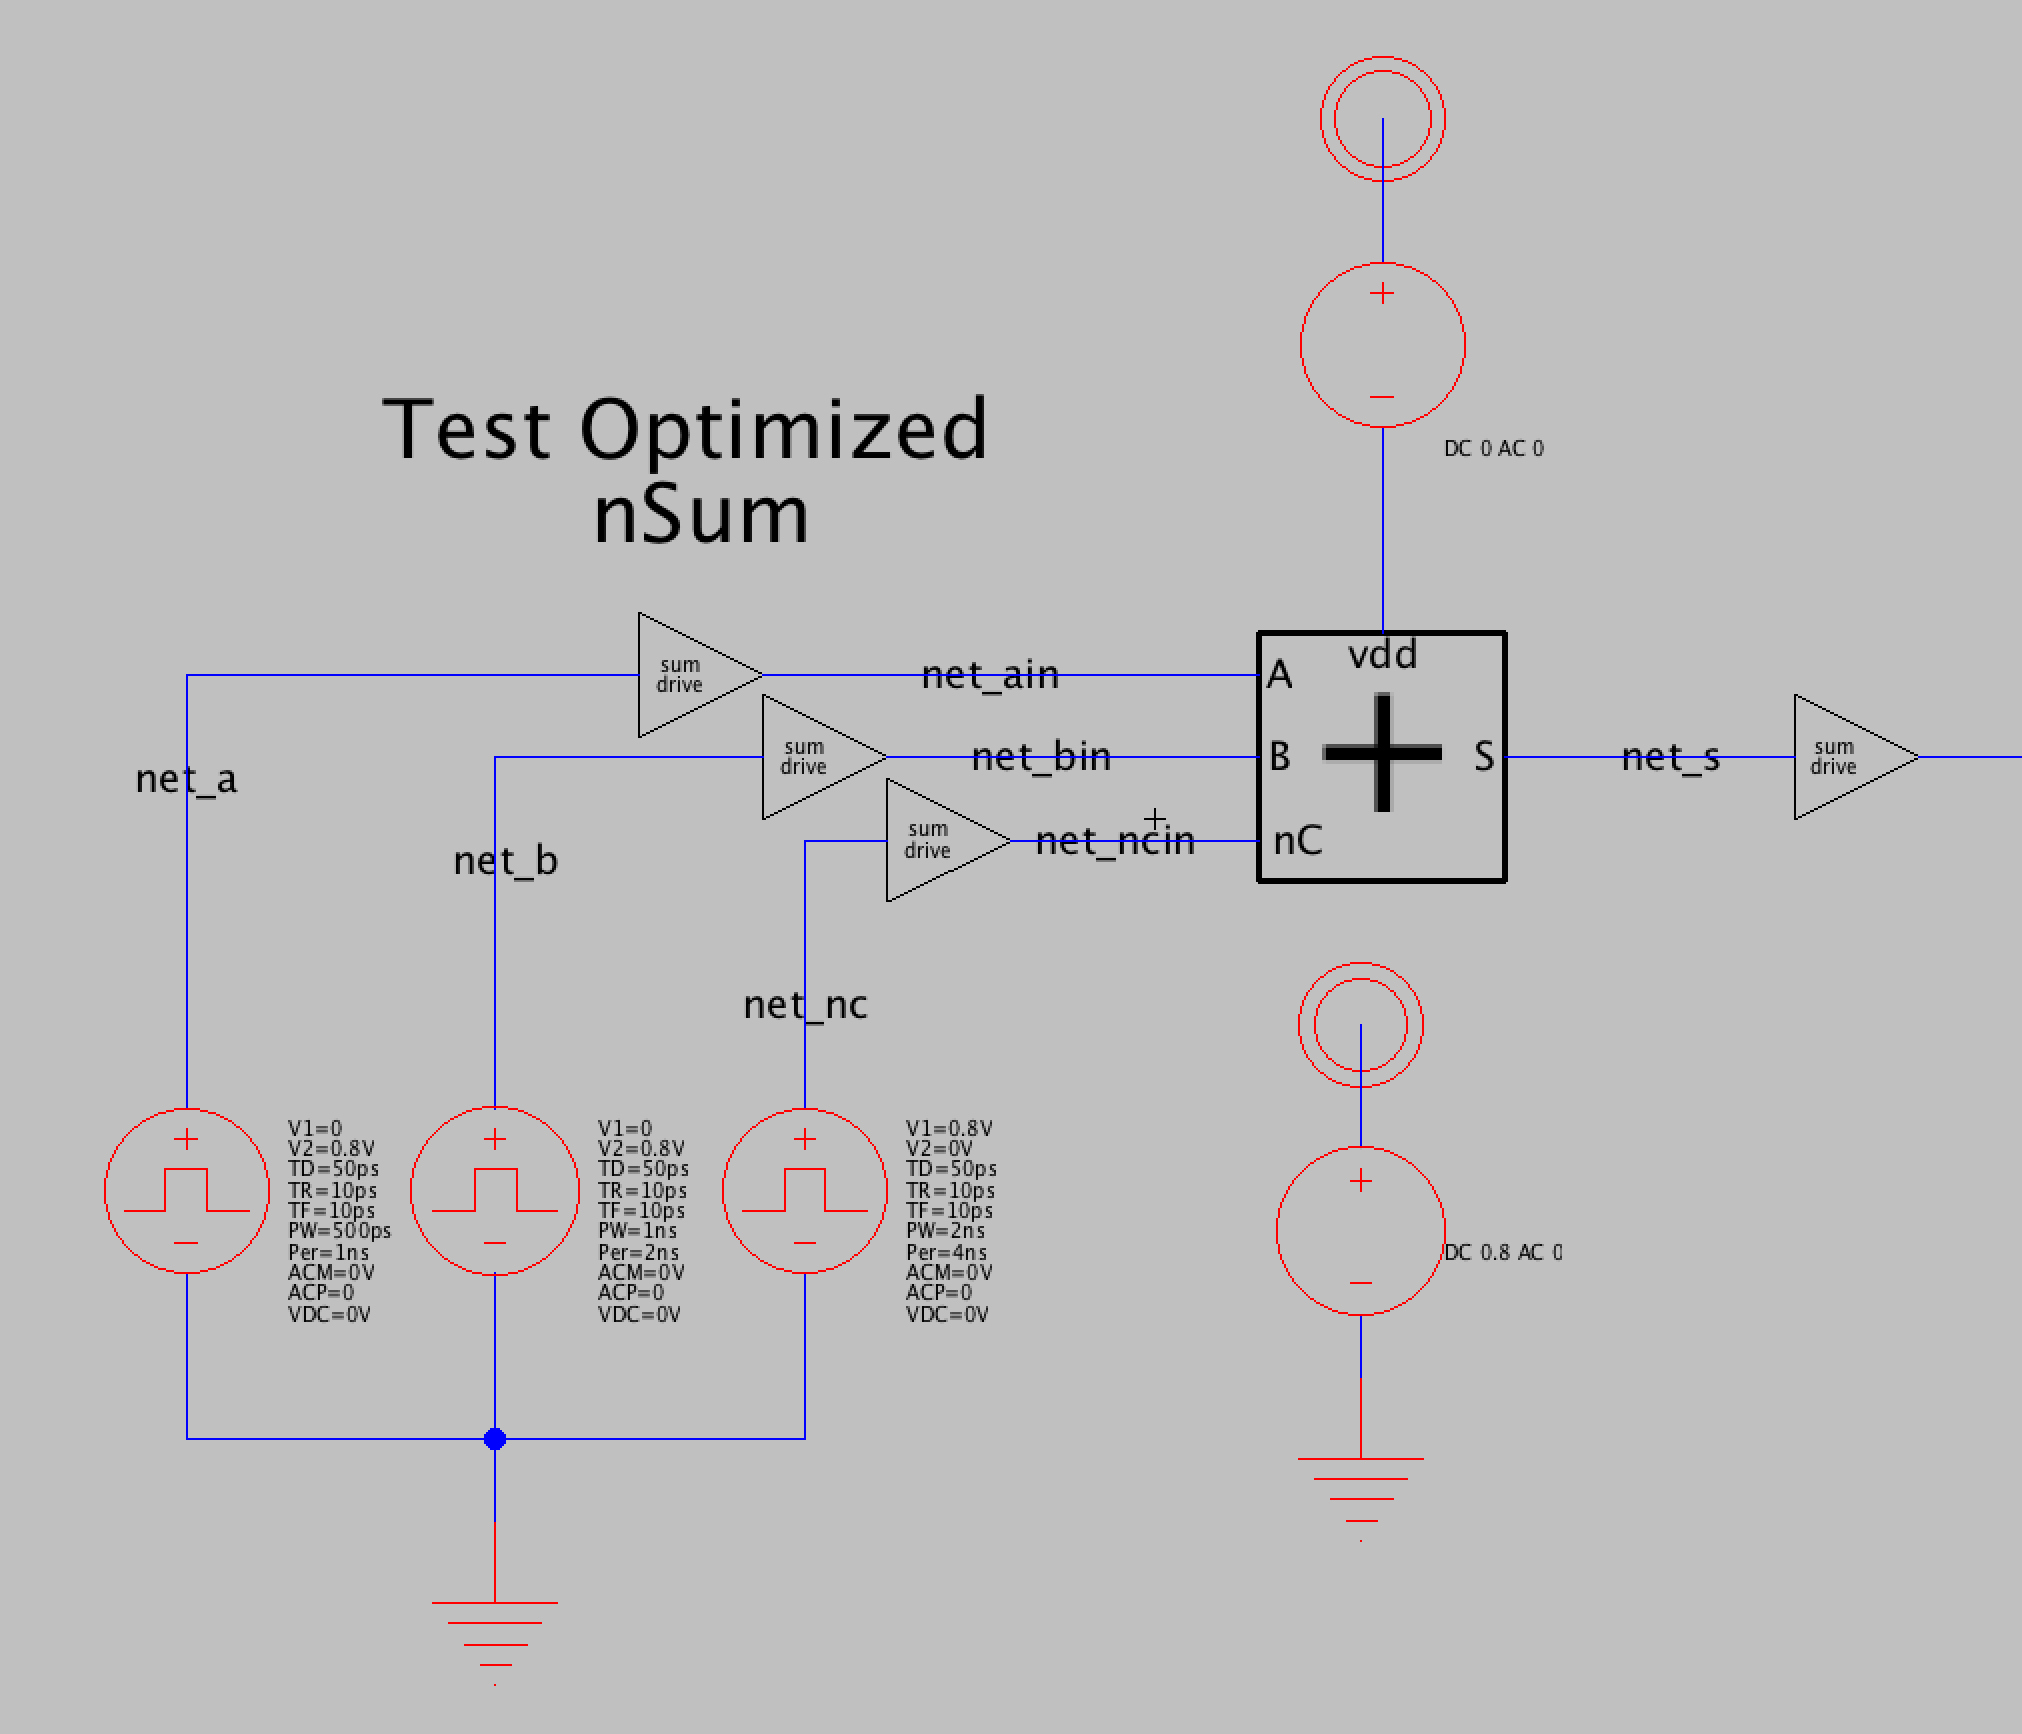
\includegraphics[width=\linewidth]{opt_screenshots/test_logic_nsum_out_sch.png}
  \caption{Schematic used to test logical correctness of nSum}
  \label{fig:test_logic_nsum_out_sch}
\end{figure}

\begin{figure}[H]
  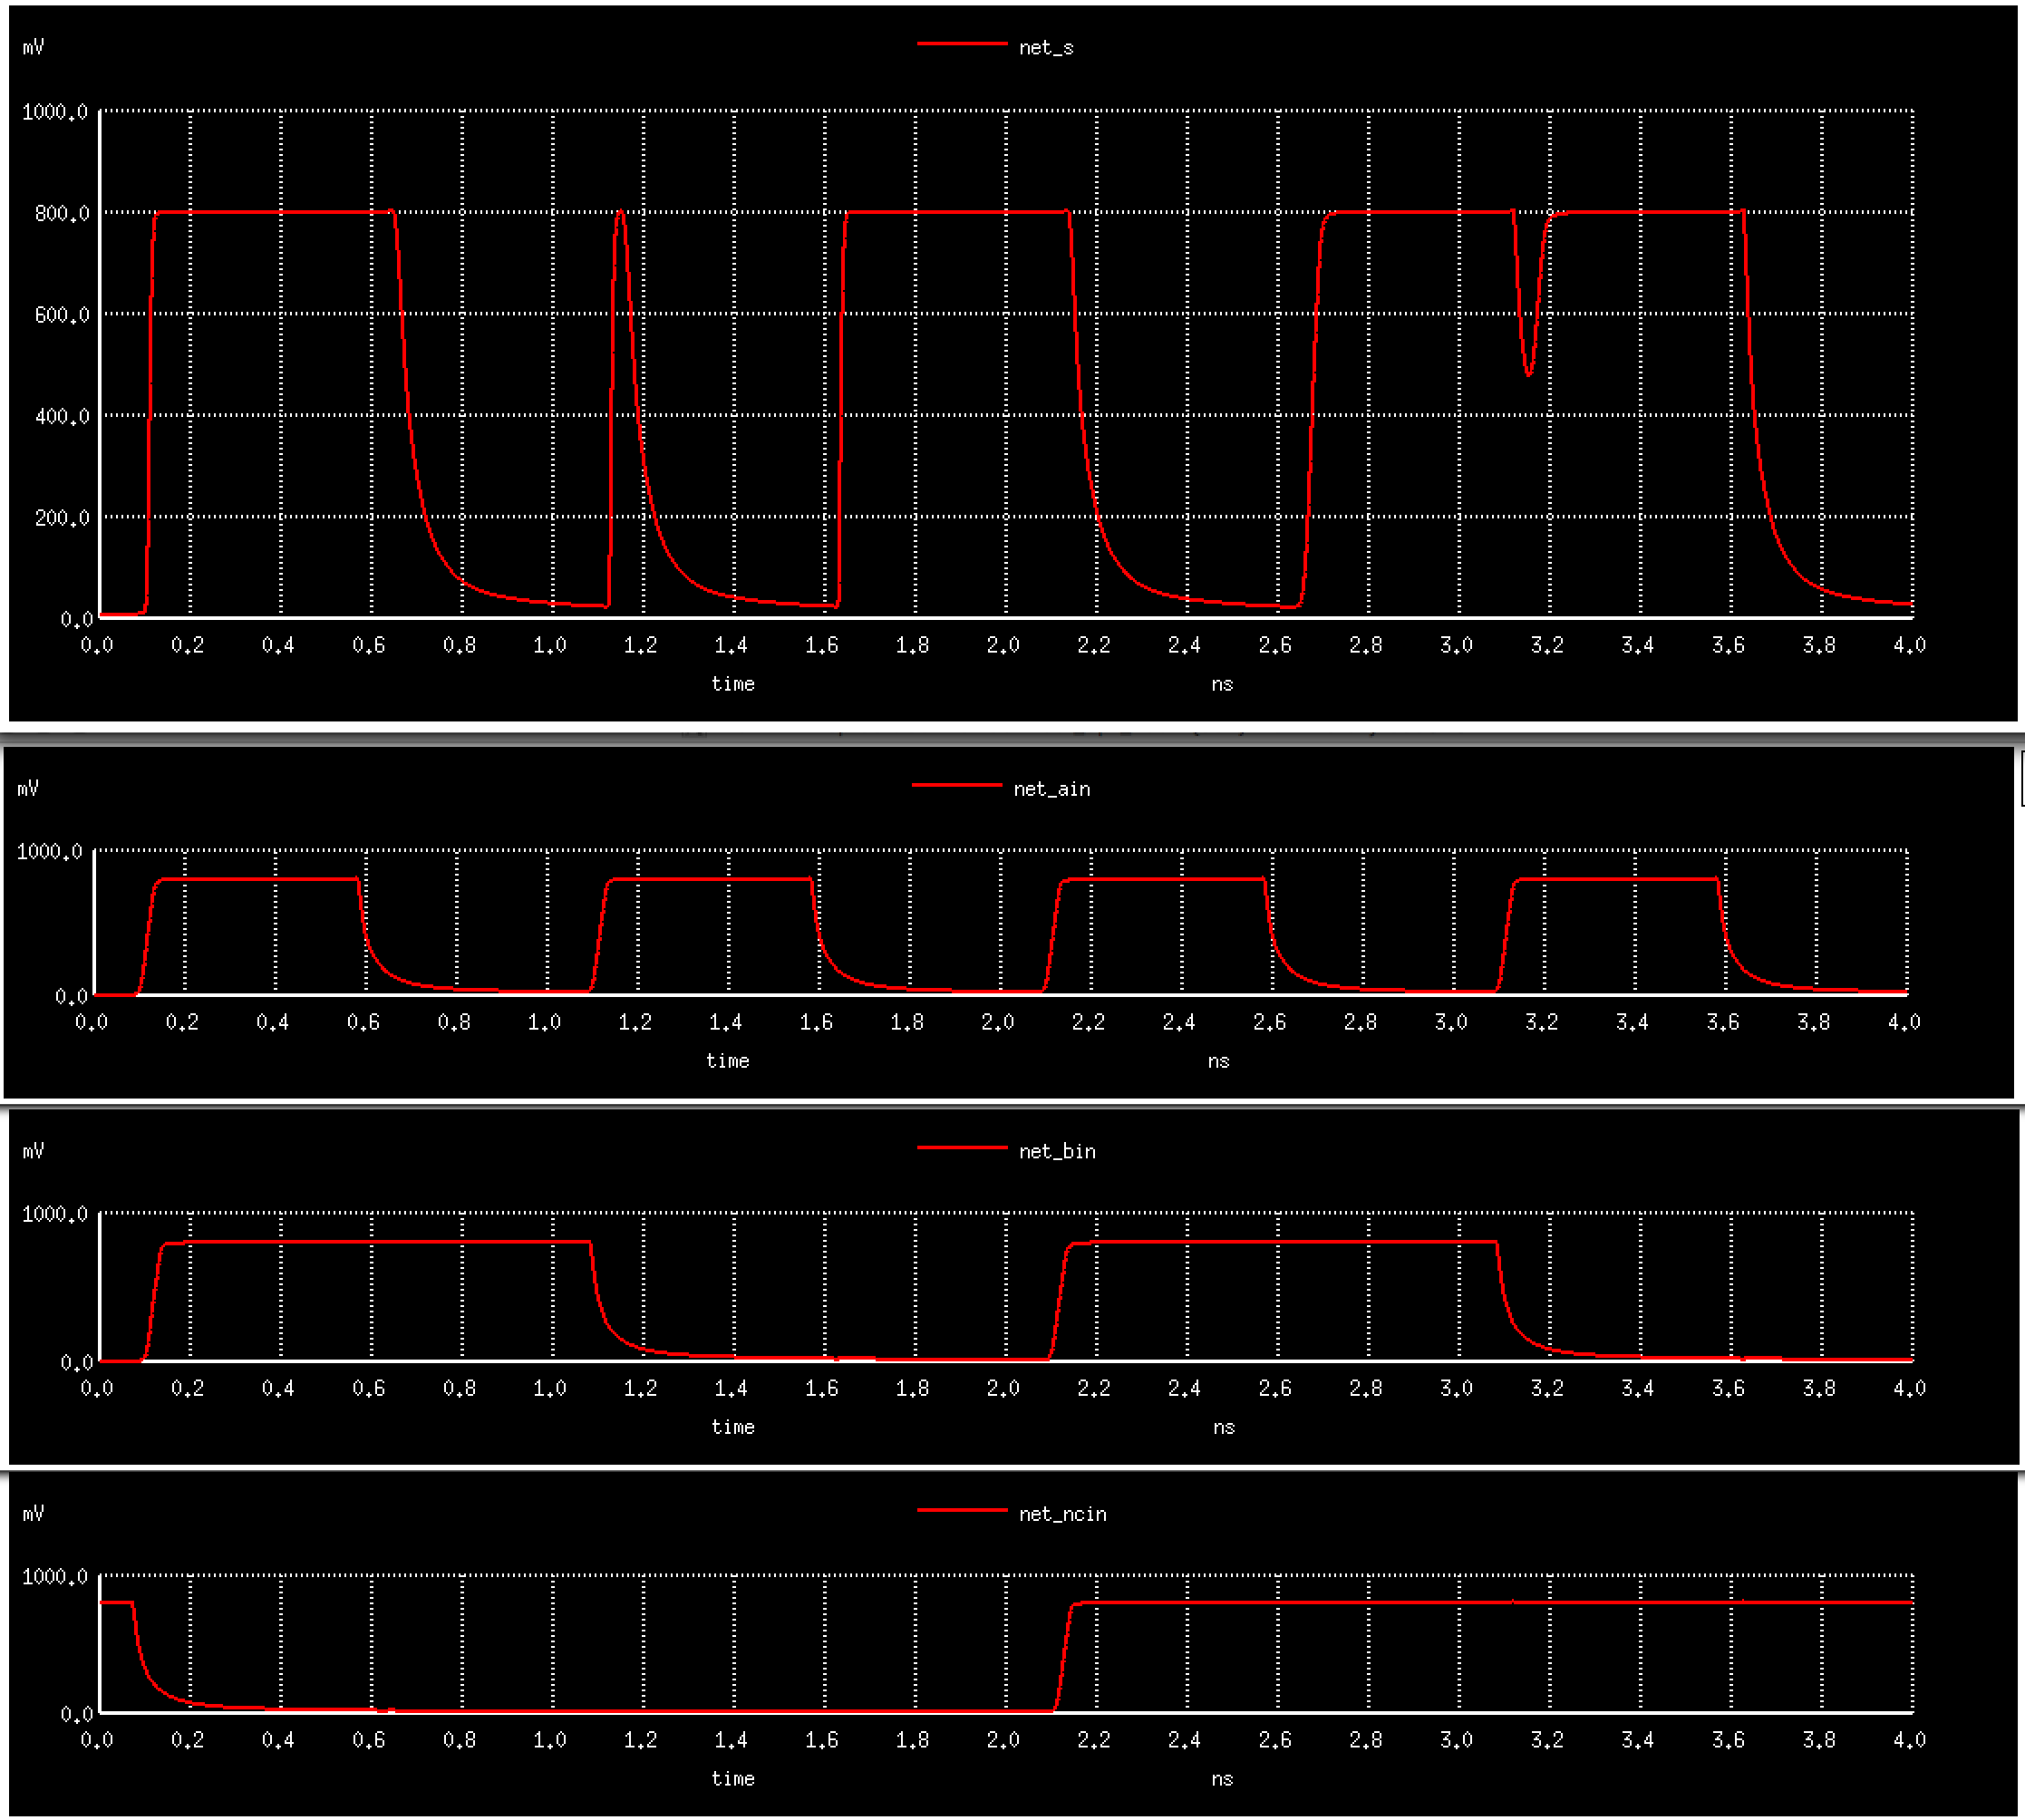
\includegraphics[width=\linewidth]{opt_screenshots/test_logic_nsum_out.png}
  \caption{Waveform showing logical correctness of nSum}
  \label{fig:test_logic_nsum_out}
\end{figure}

\subsubsection{Carry}
\begin{figure}[H]
  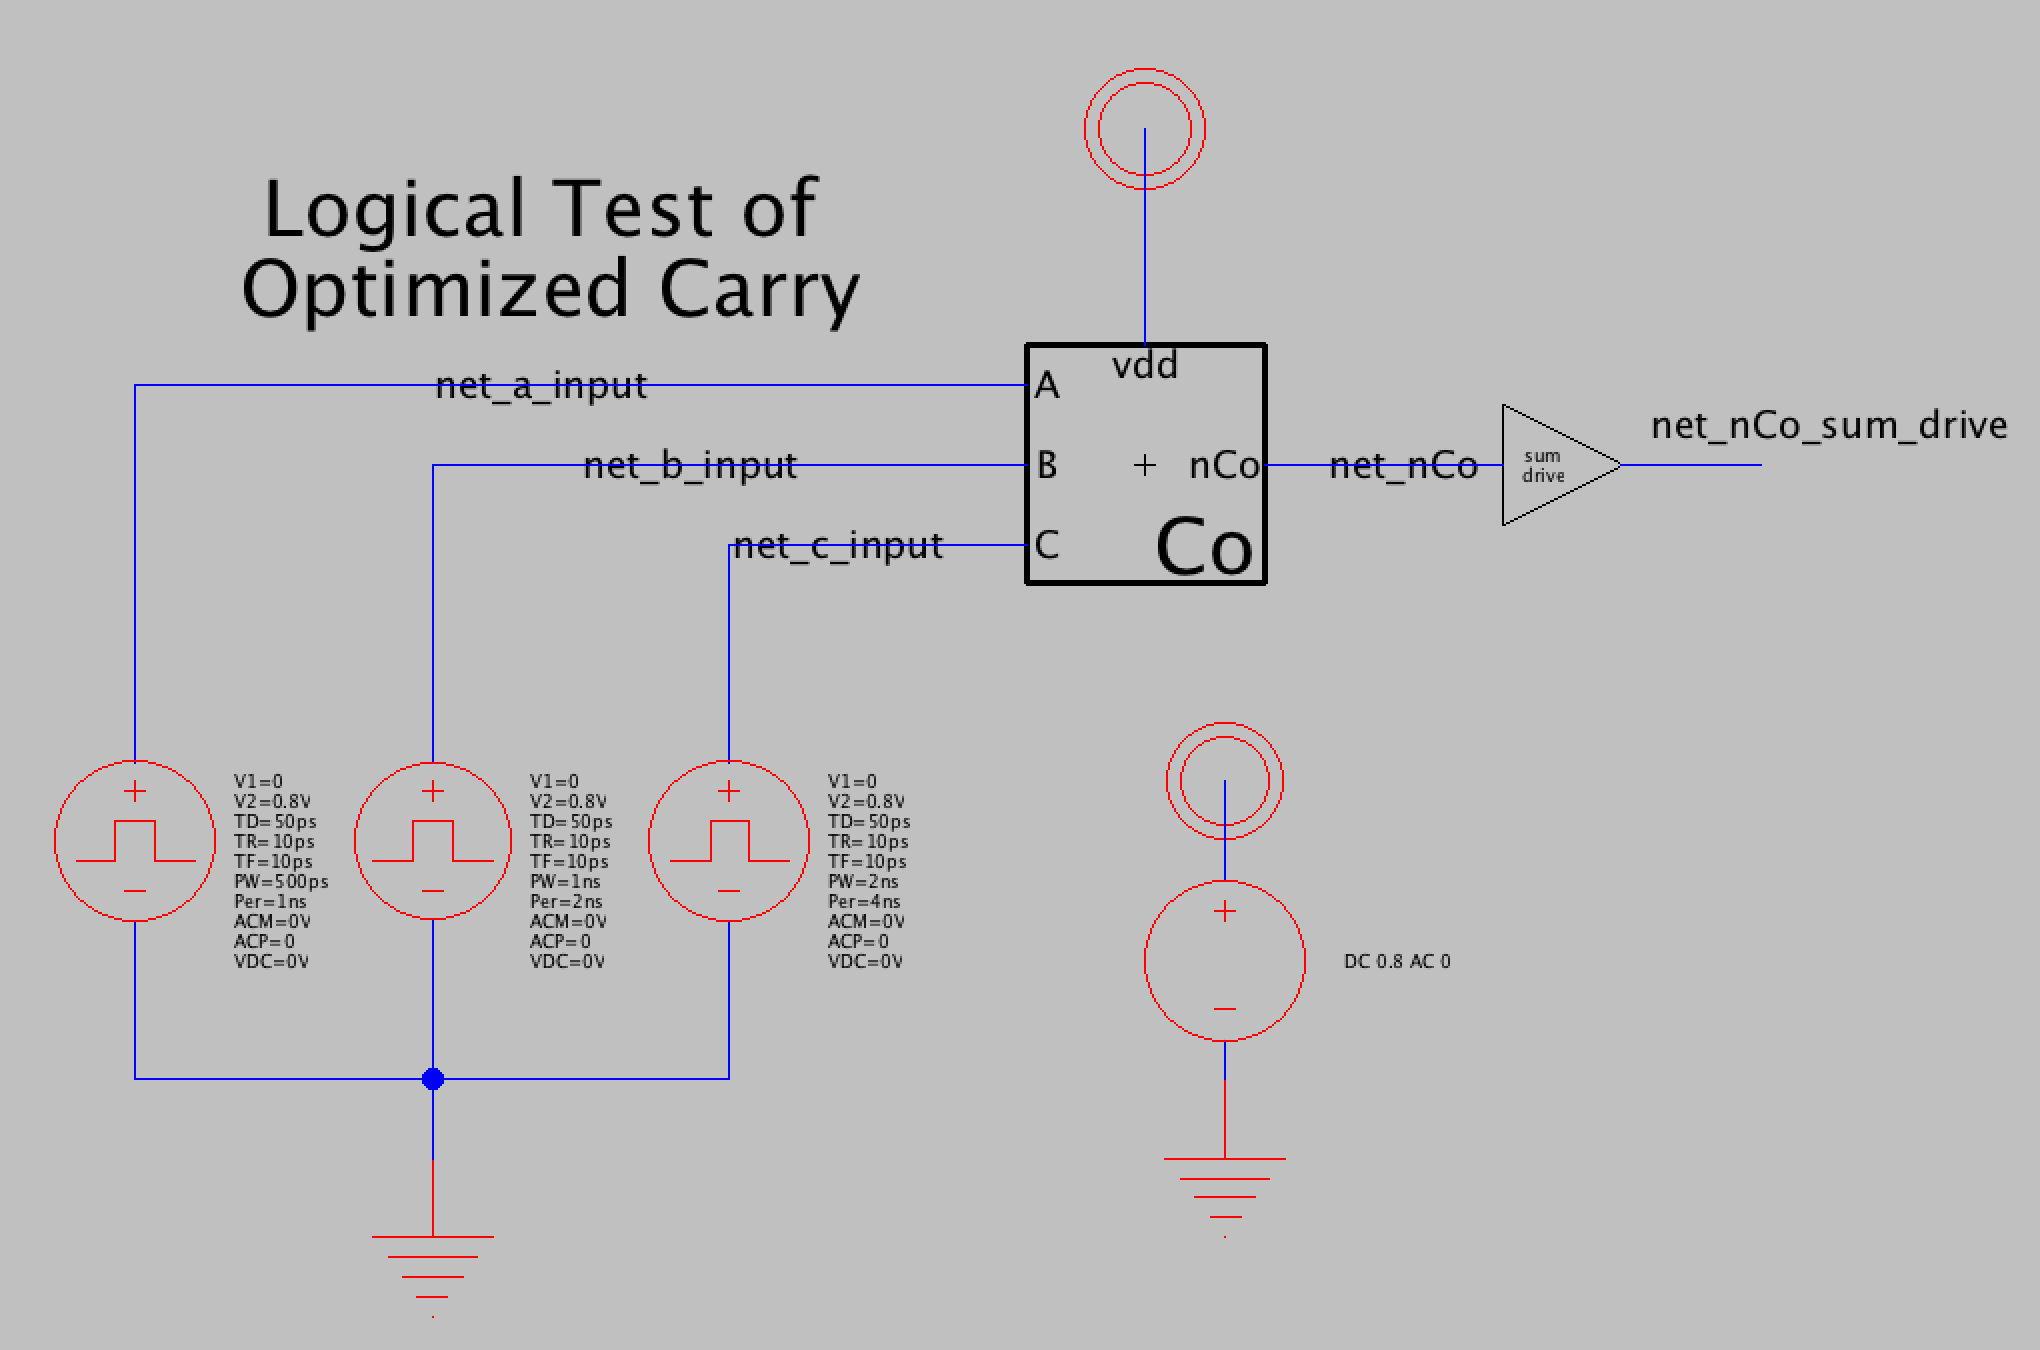
\includegraphics[width=\linewidth]{opt_screenshots/test_logic_opt_carry_sch.png}
  \caption{Schematic used to test logical correctness of Carry}
  \label{fig:test_logic_opt_carry_sch}
\end{figure}

\begin{figure}[H]
  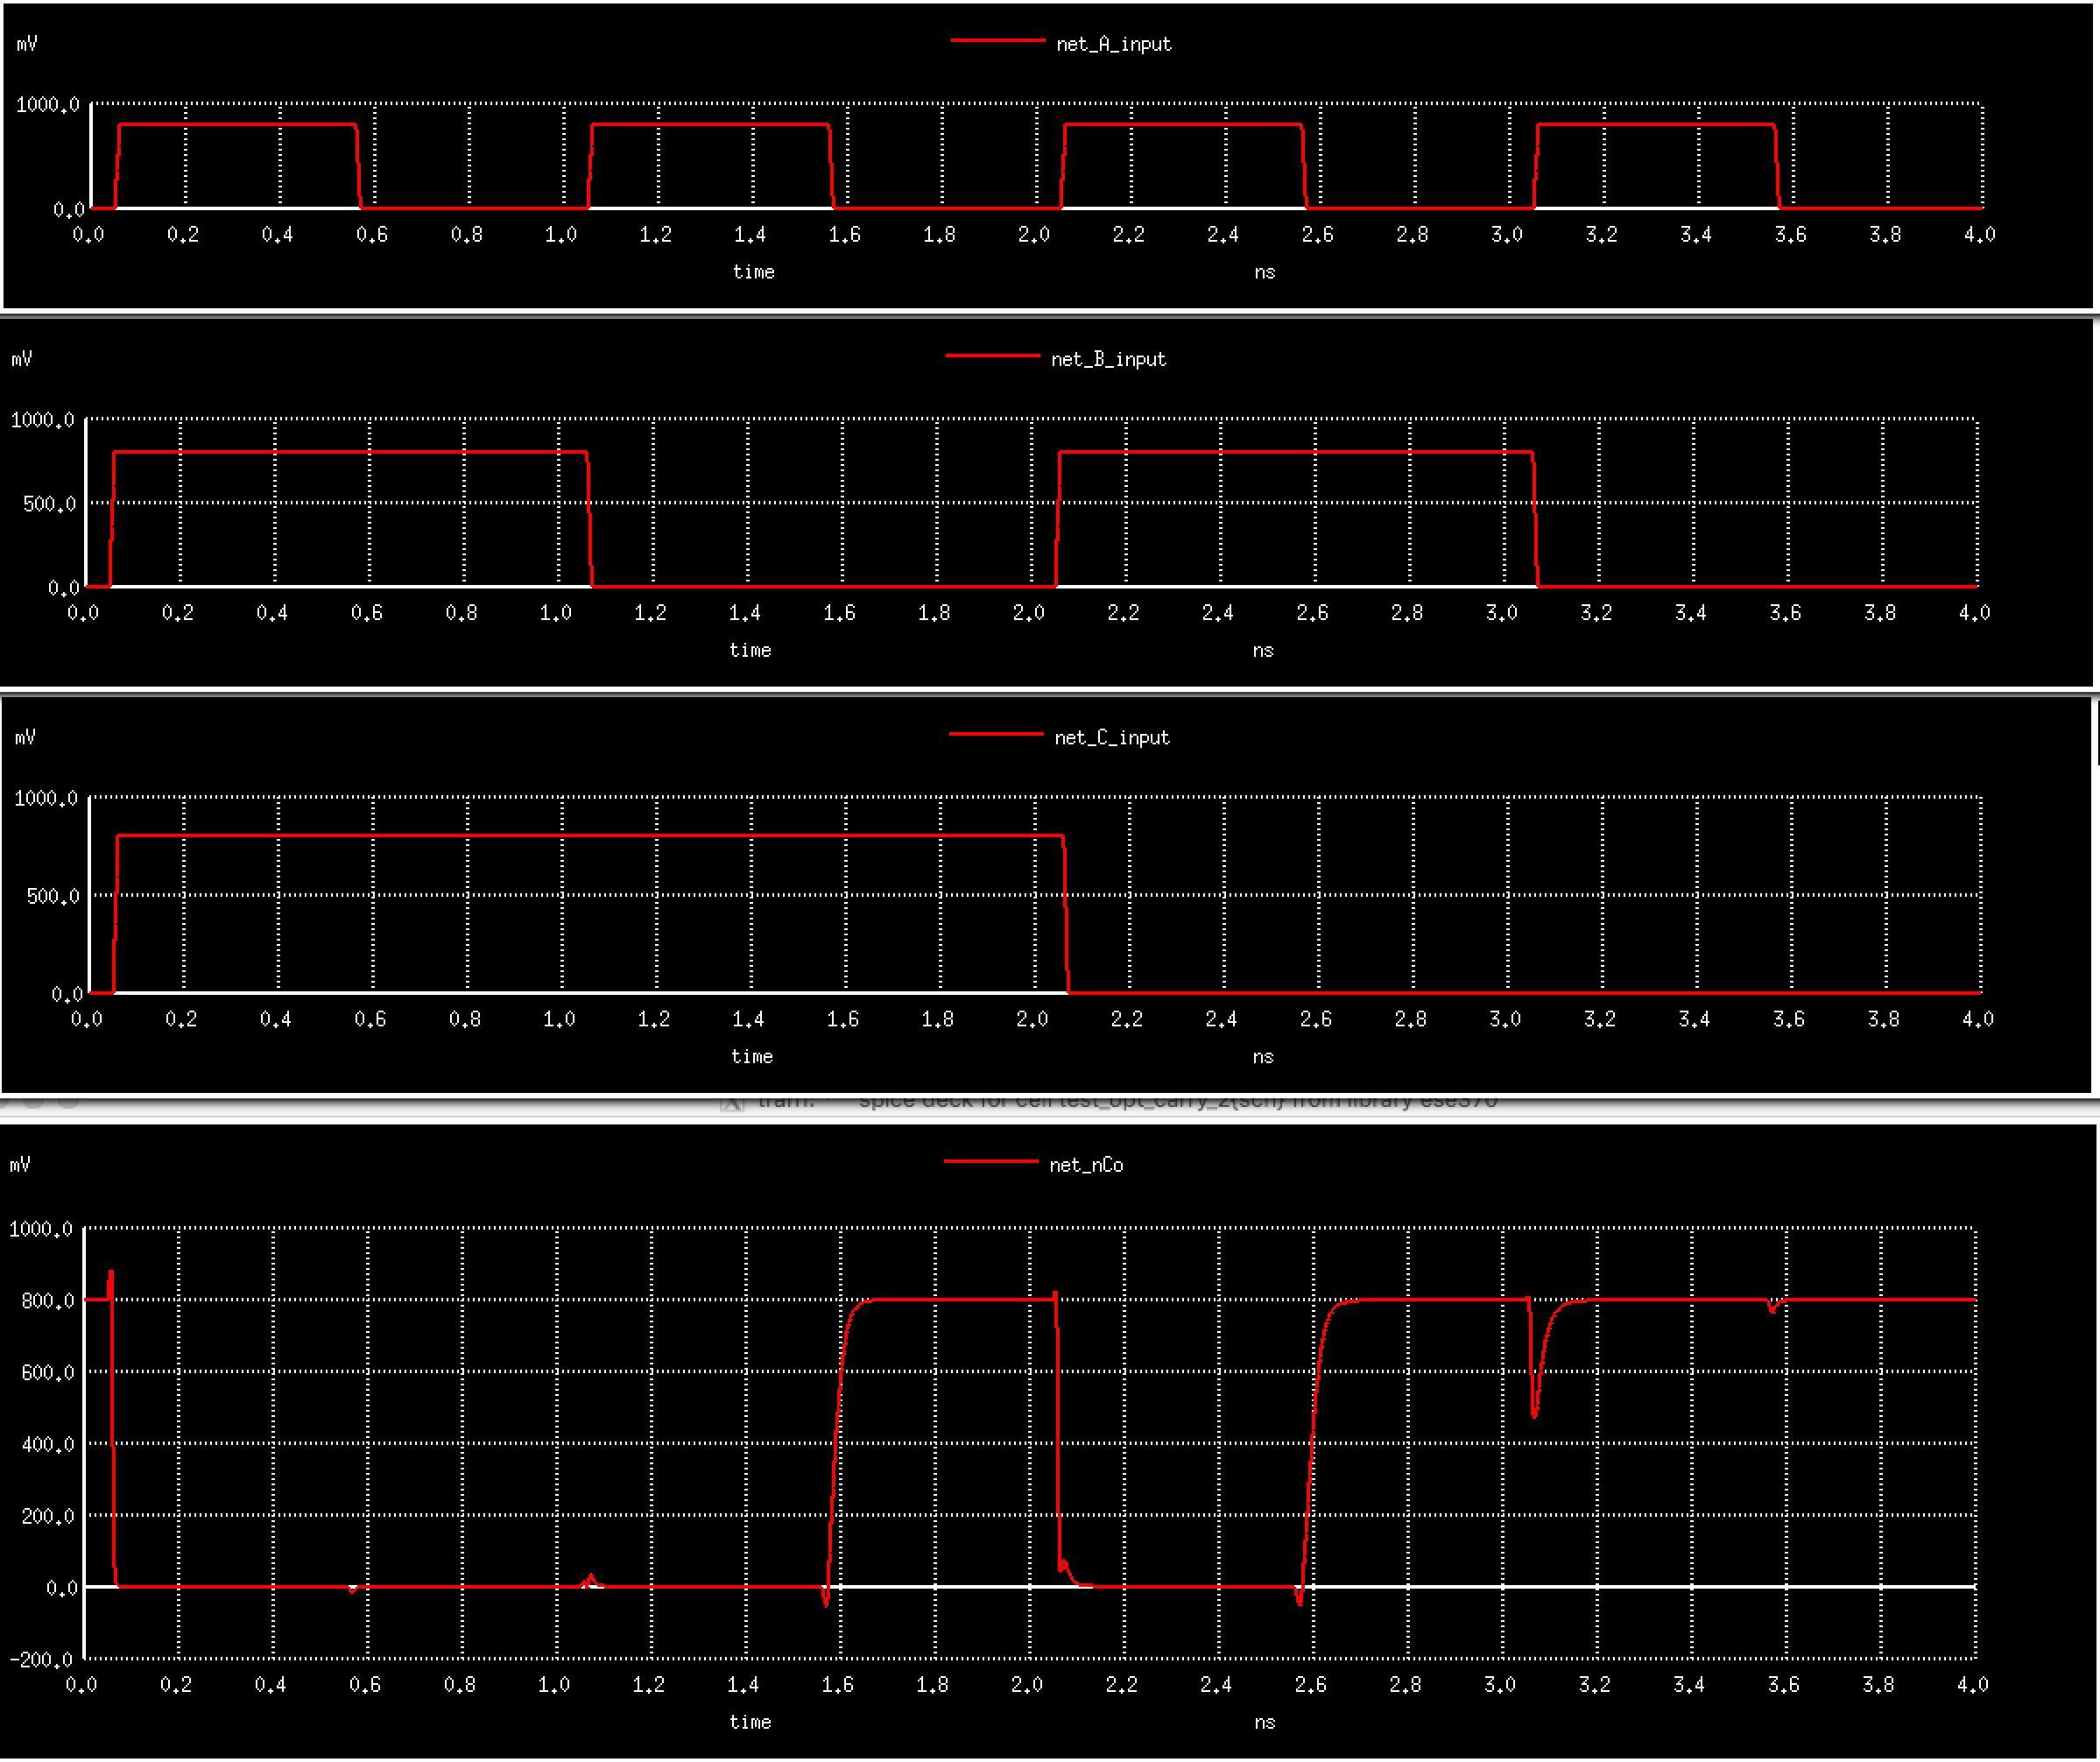
\includegraphics[width=\linewidth]{opt_screenshots/test_logic_real_carry_out.png}
  \caption{Waveform showing logical correctness of Carry}
  \label{fig:test_logic_real_carry_out}
\end{figure}

\subsubsection{nCarry}
\begin{figure}[H]
  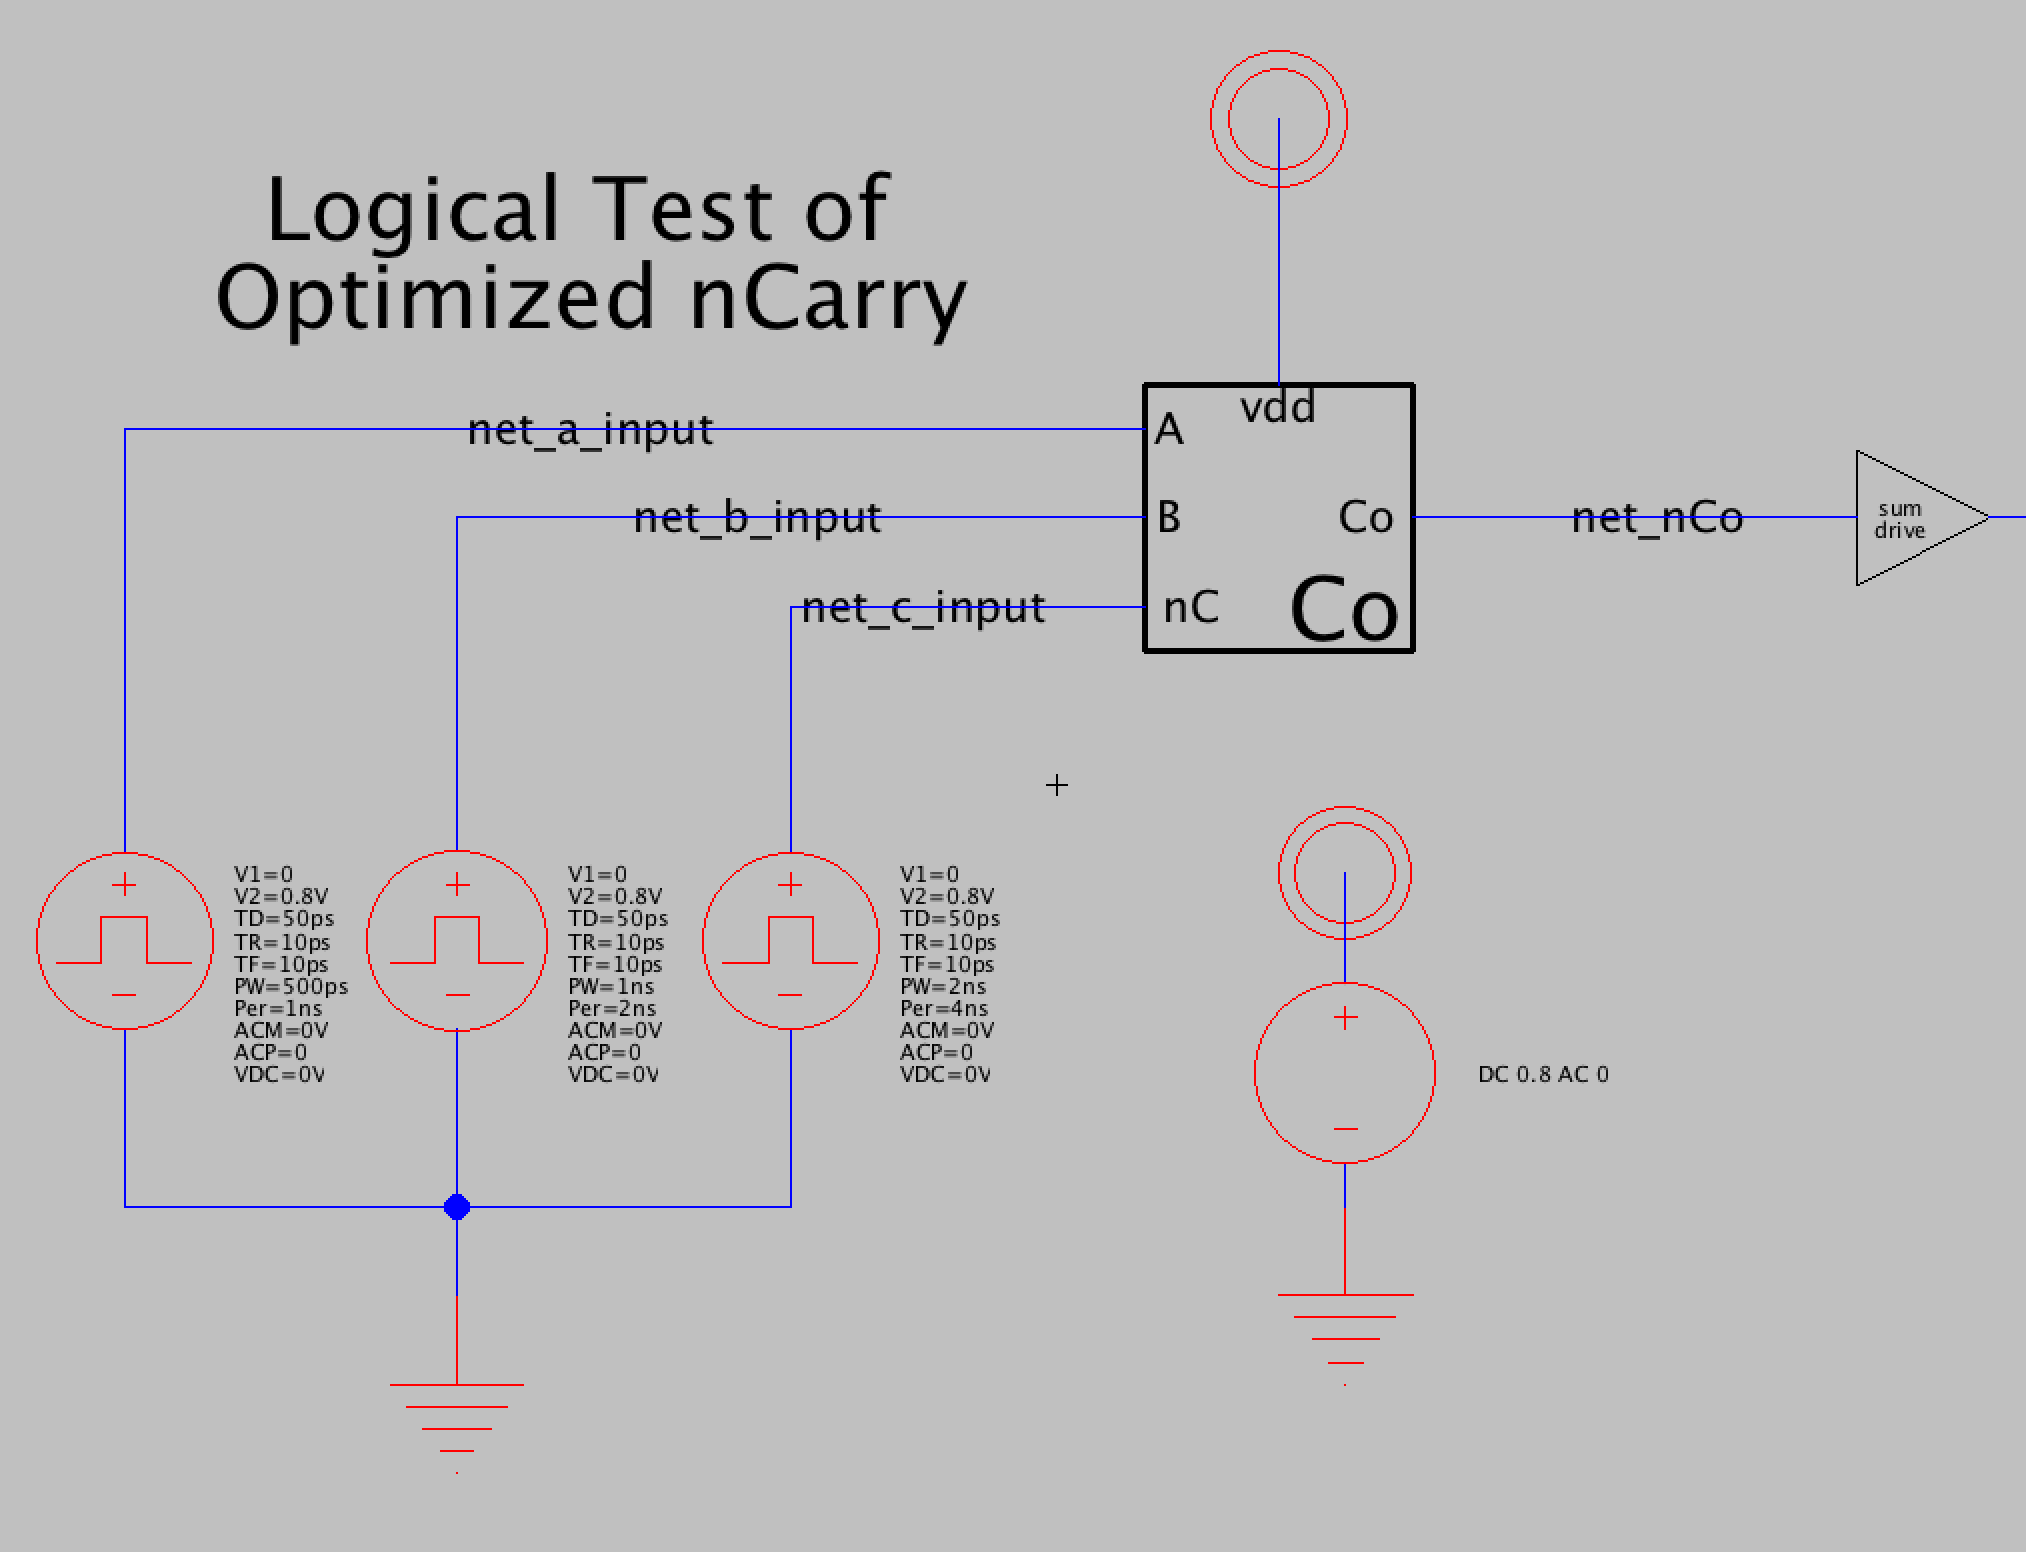
\includegraphics[width=\linewidth]{opt_screenshots/test_logic_opt_ncarry_sch.png}
  \caption{Schematic used to test logical correctness of nCarry}
  \label{fig:test_logic_opt_ncarry_sch}
\end{figure}

\begin{figure}[H]
  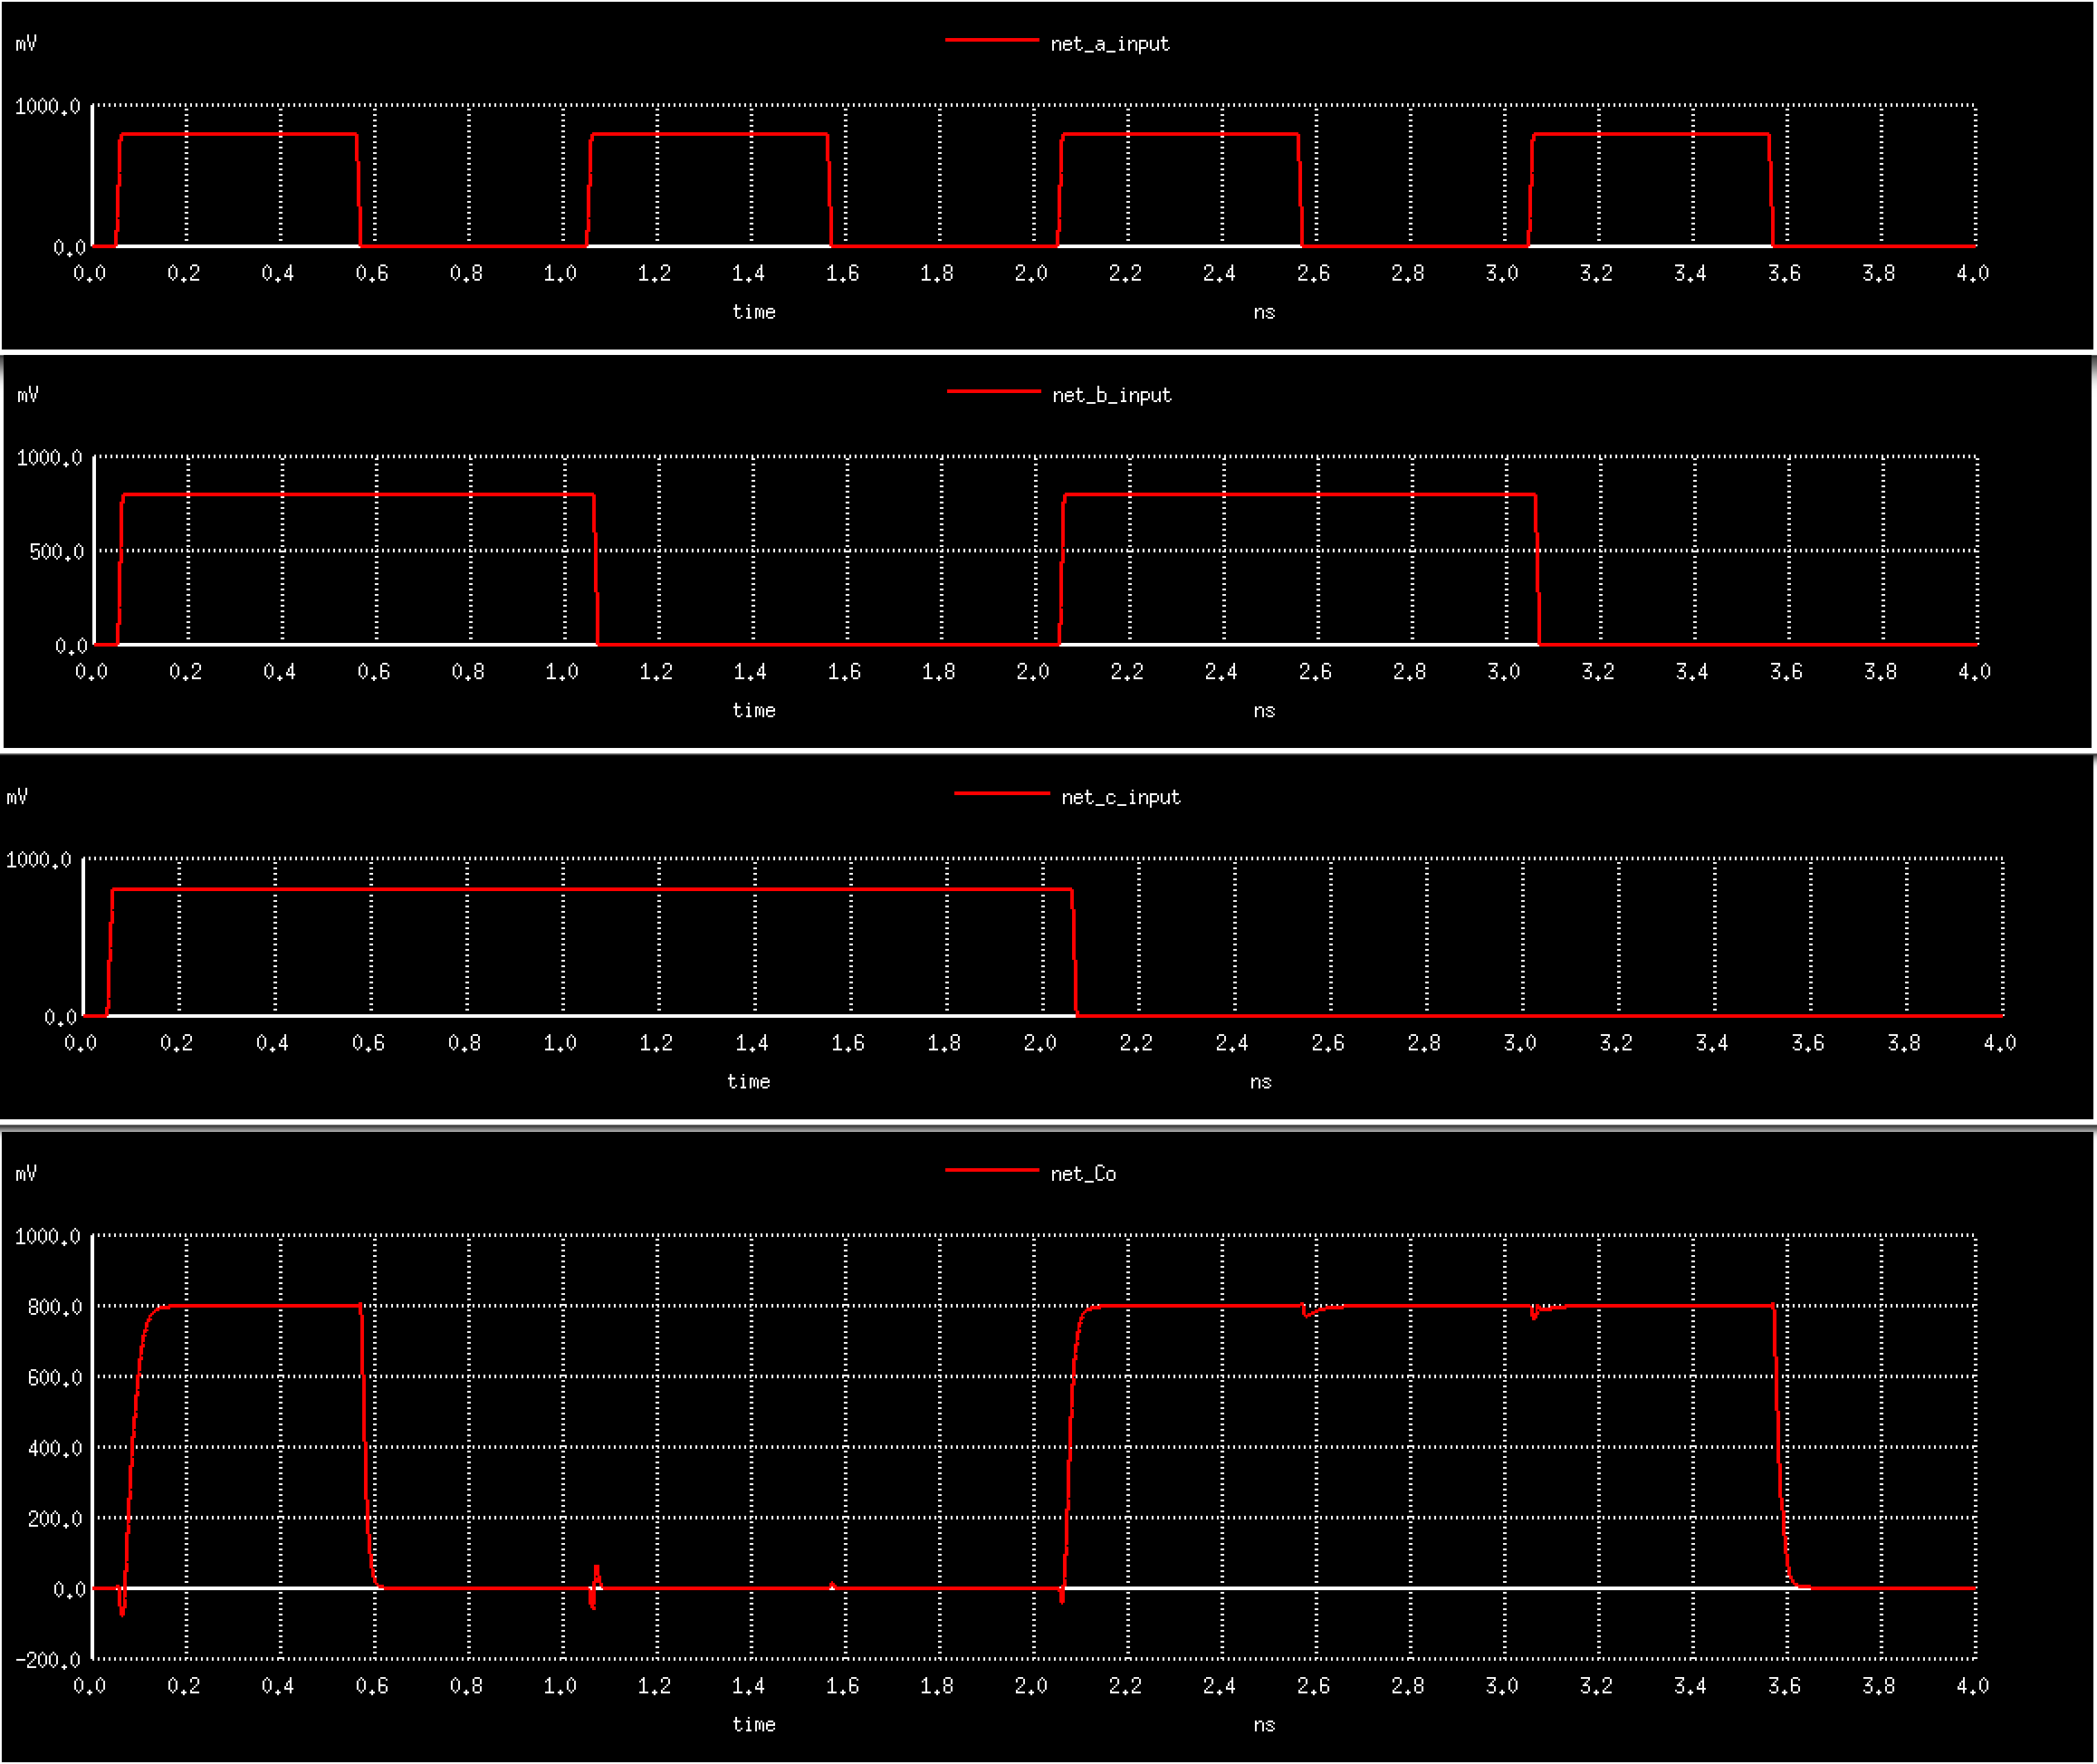
\includegraphics[width=\linewidth]{opt_screenshots/test_logic_real_ncarry_out.png}
  \caption{Waveform showing logical correctness of nCarry}
  \label{fig:test_logic_real_ncarry_out}
\end{figure}

\subsubsection{1-bit Adder}
\begin{figure}[H]
  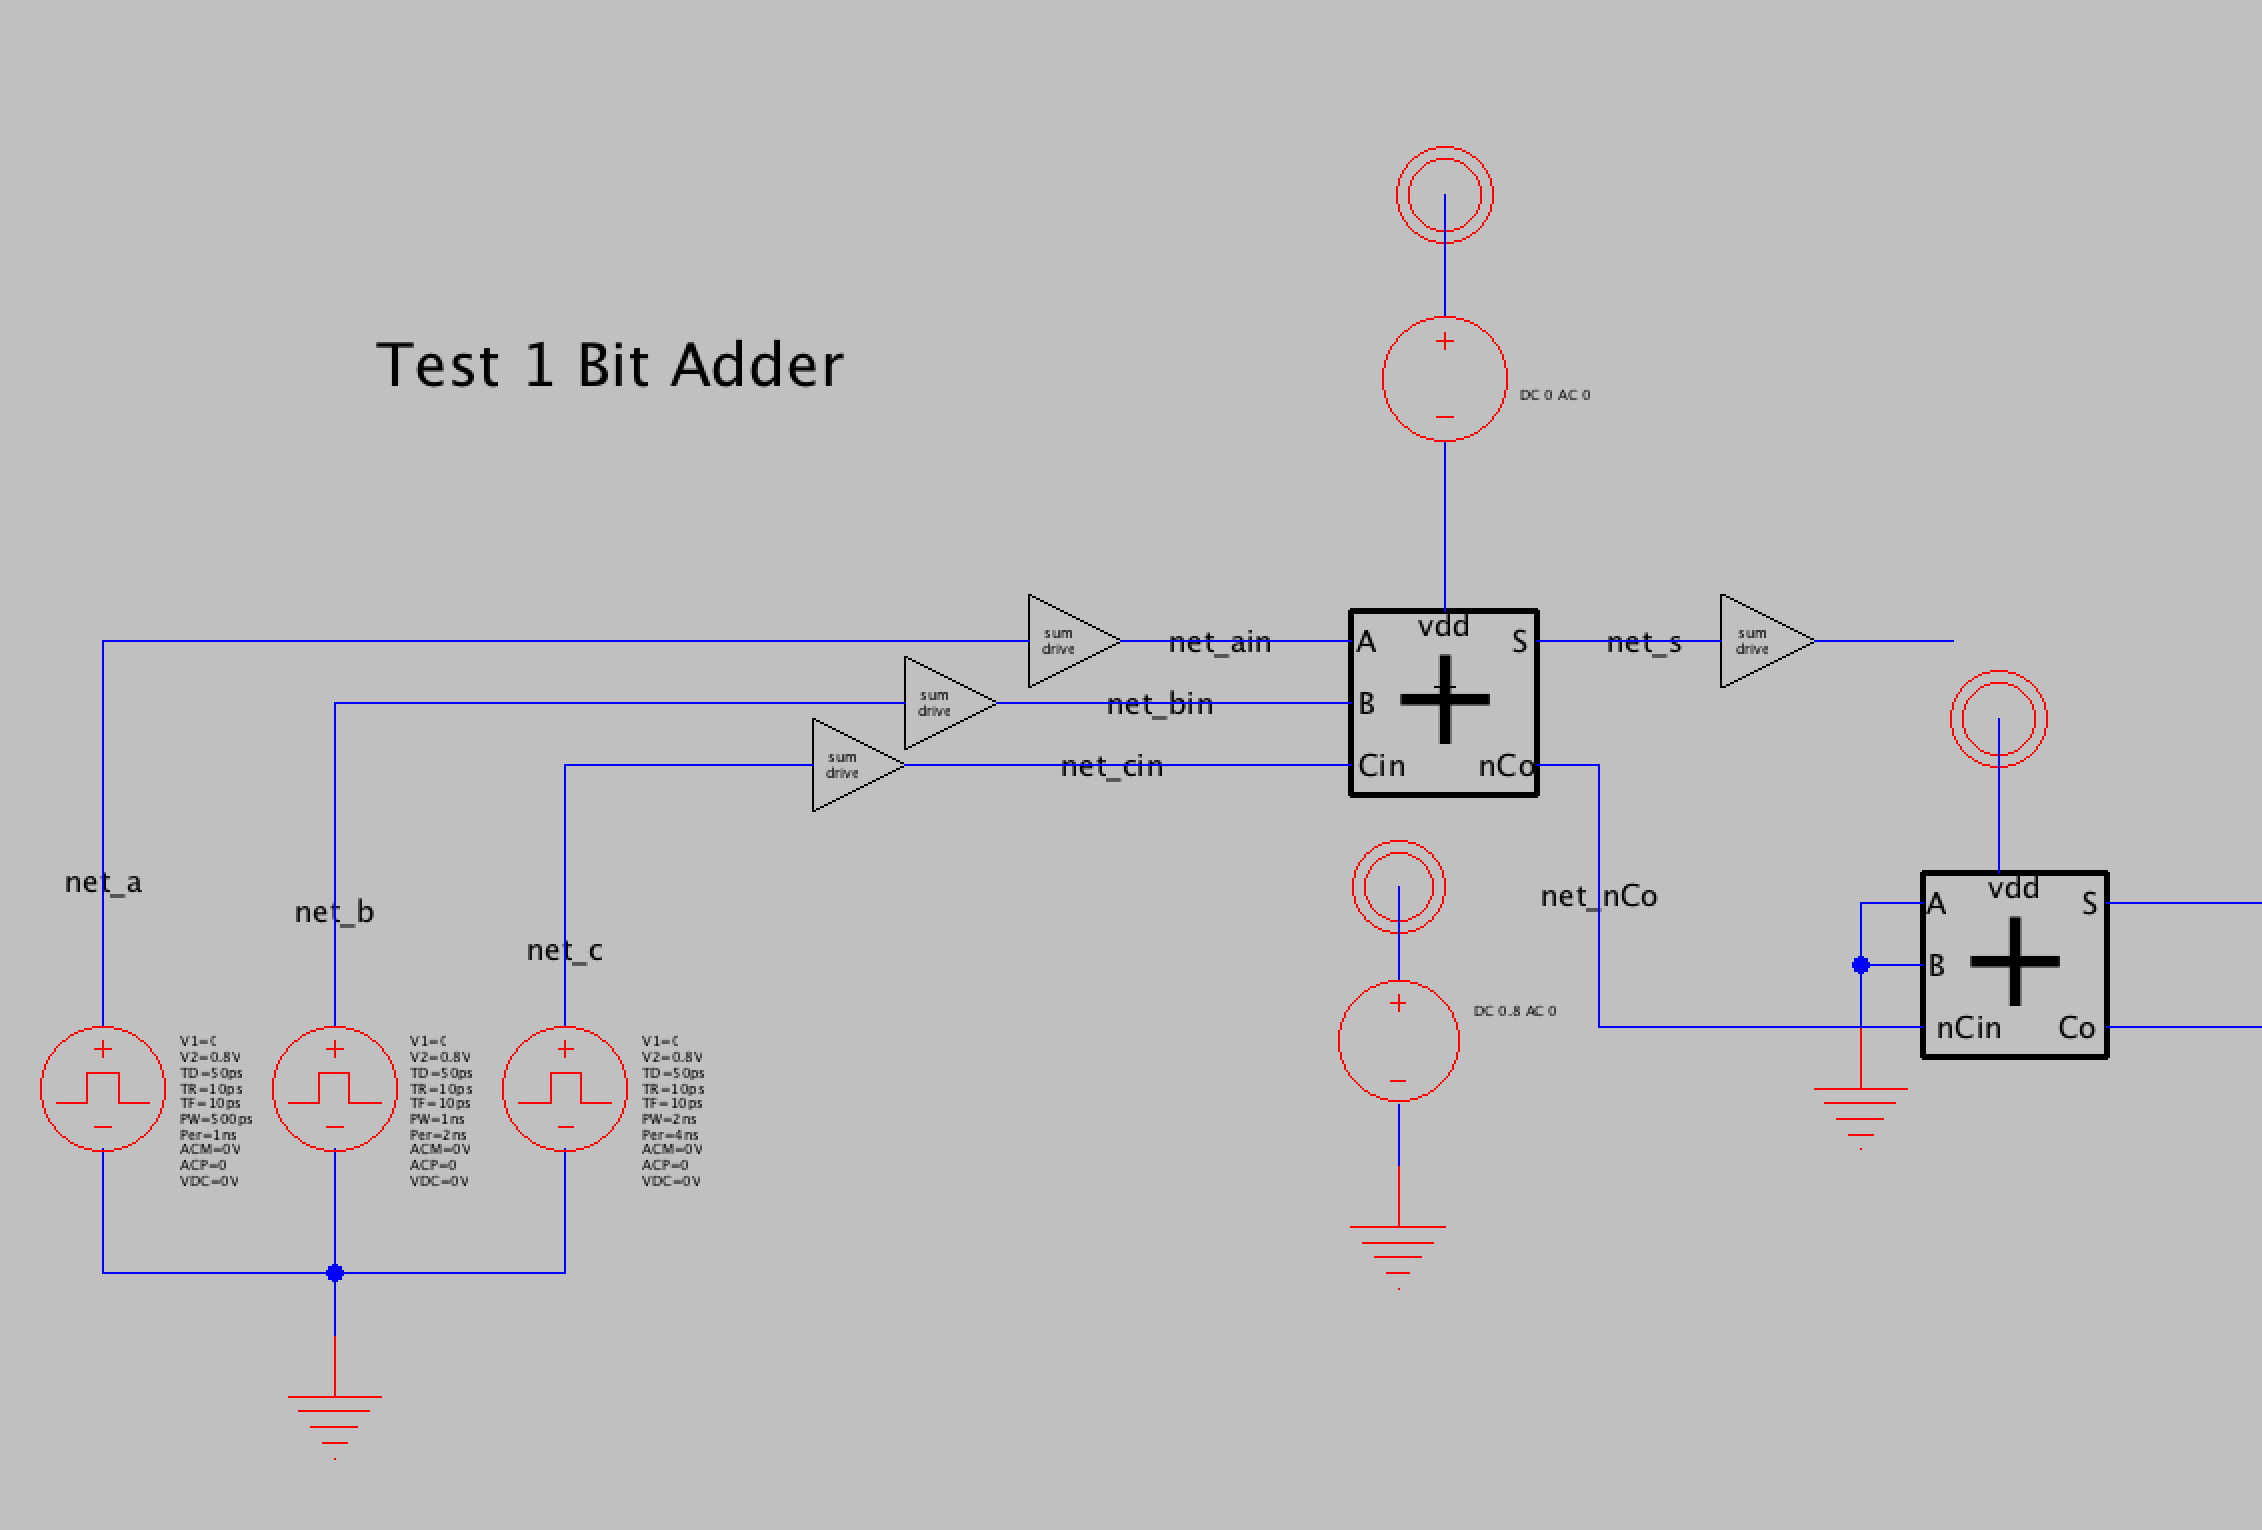
\includegraphics[width=\linewidth]{opt_screenshots/test_logic_1b_adder_sch.png}
  \caption{Schematic used to test logical correctness of the 1-bit Adder}
  \label{fig:test_logic_1b_adder_sch}
\end{figure}

\begin{figure}[H]
  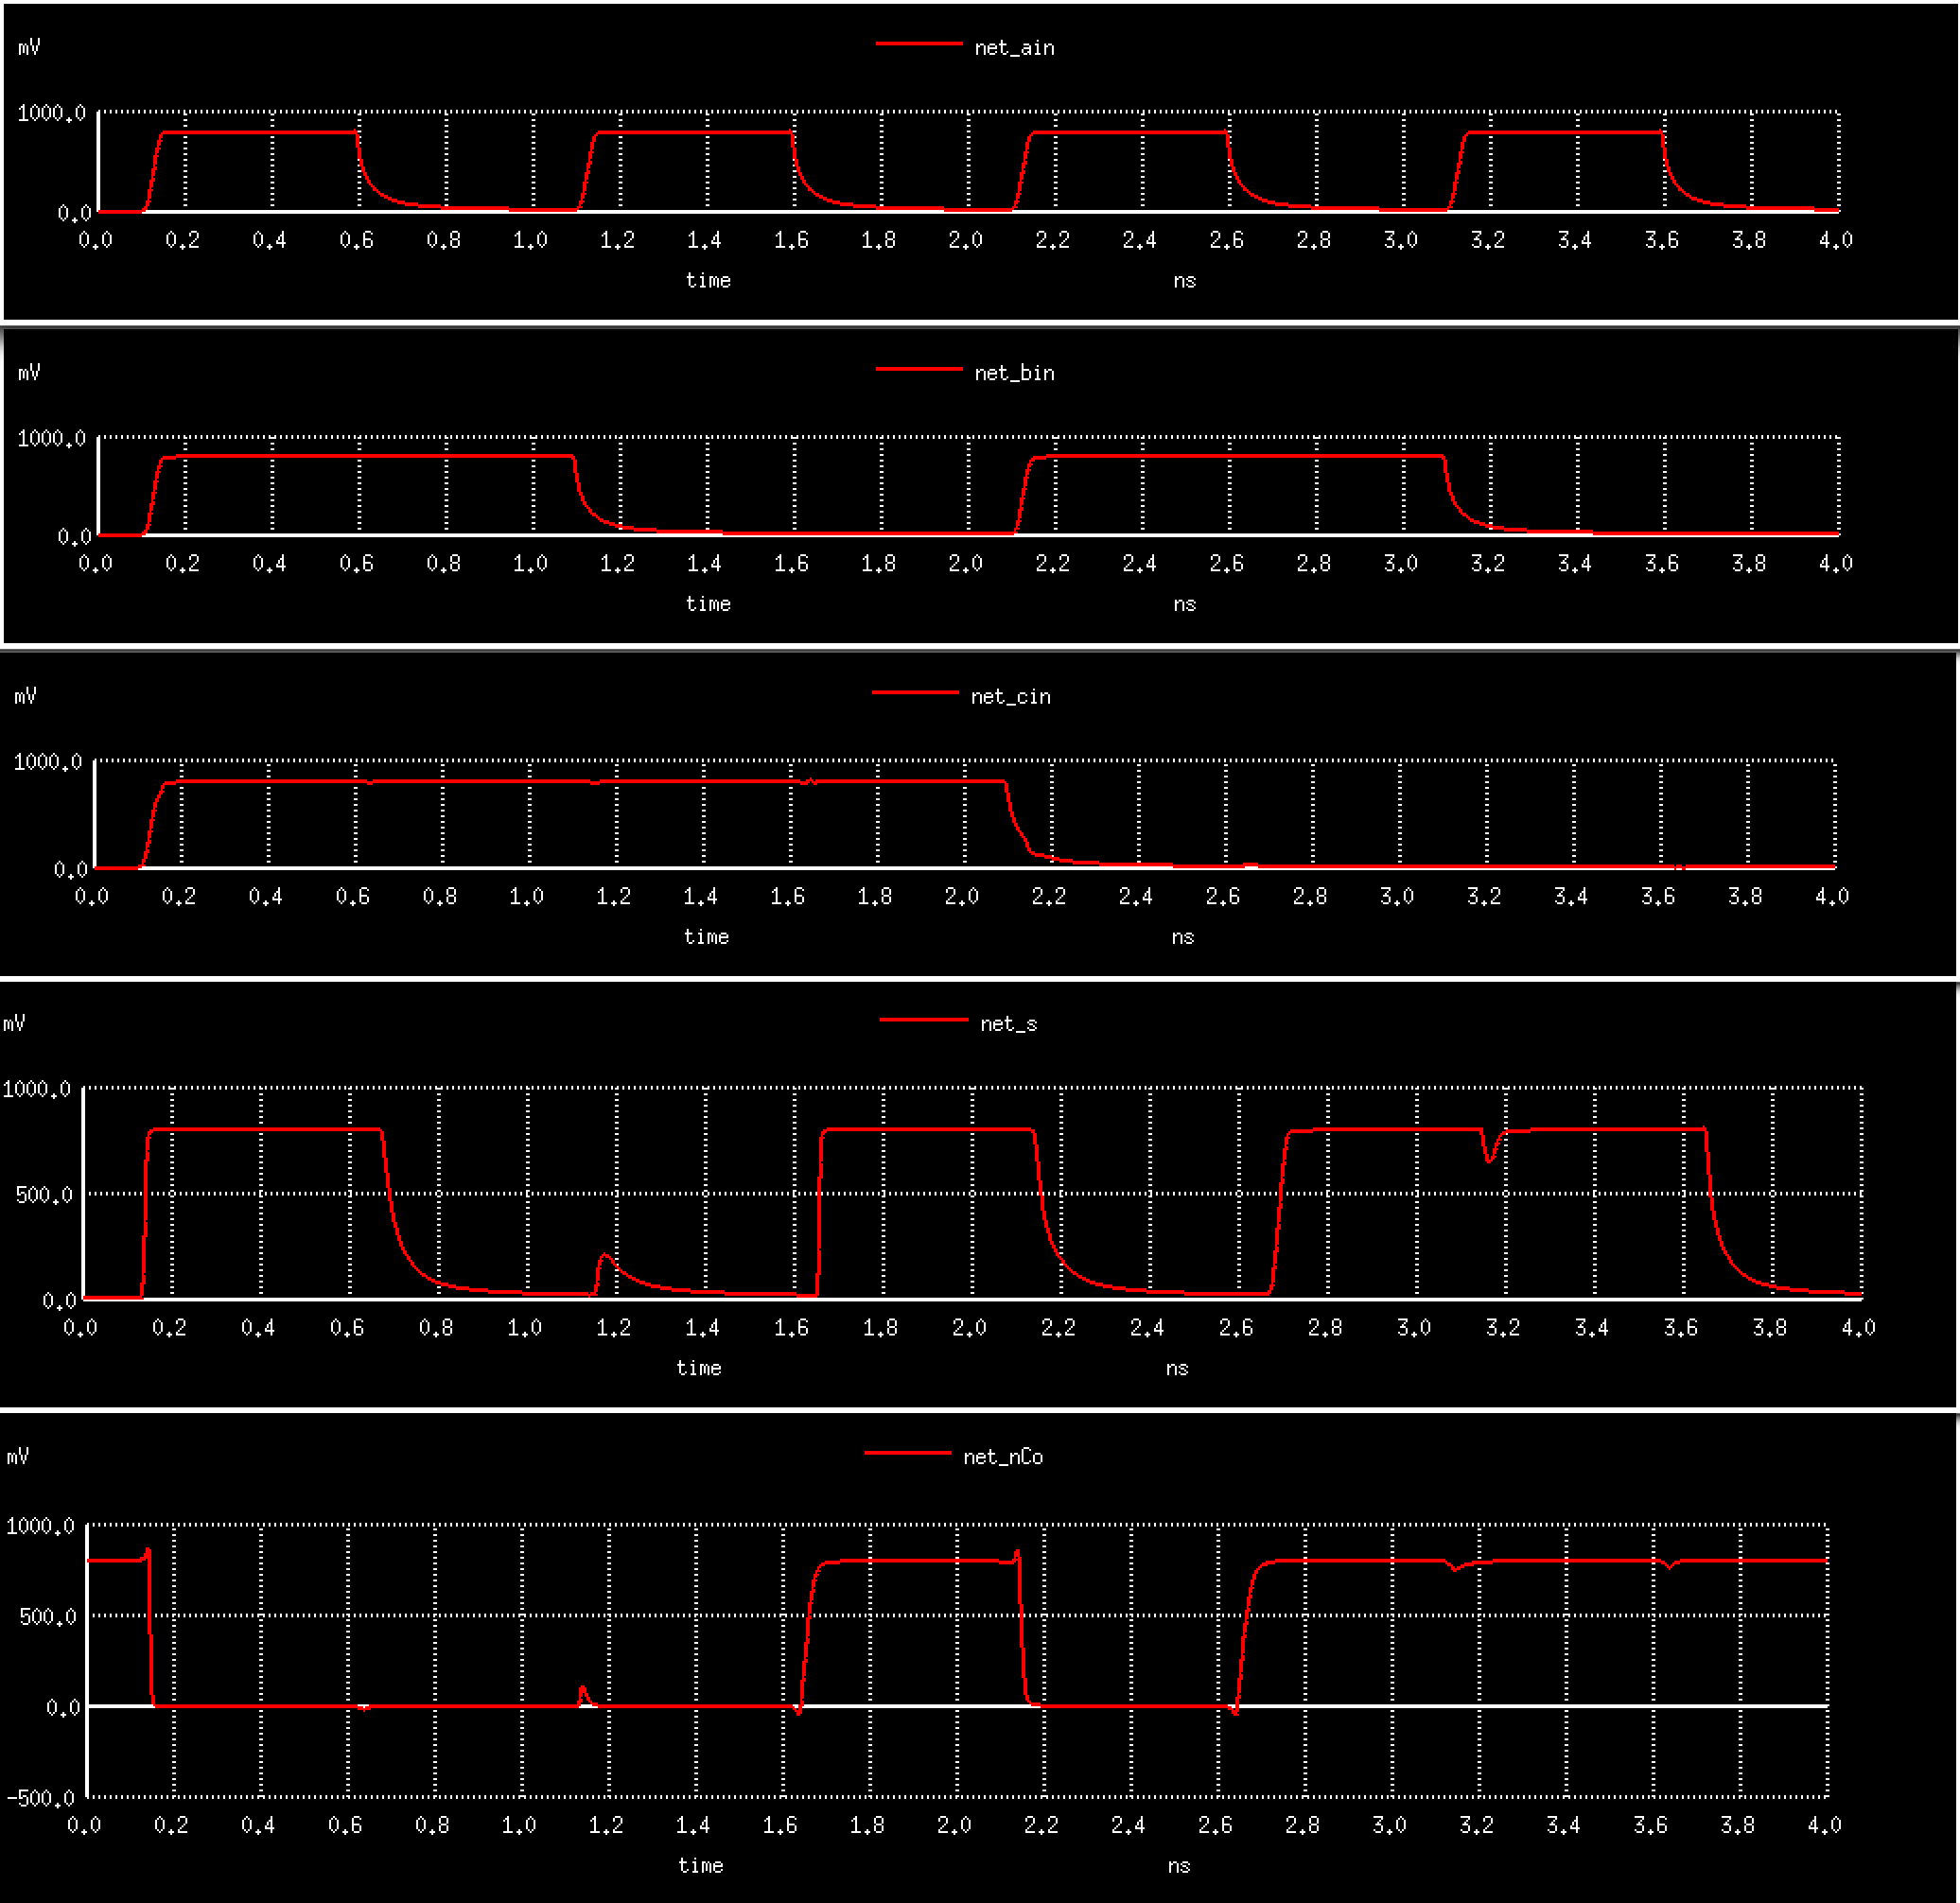
\includegraphics[width=\linewidth]{opt_screenshots/test_logic_1b_adder.png}
  \caption{Waveform showing logical correctness of the 1-bit Adder}
  \label{fig:test_logic_1b_adder}
\end{figure}

\subsubsection{1-bit nAdder}
\begin{figure}[H]
  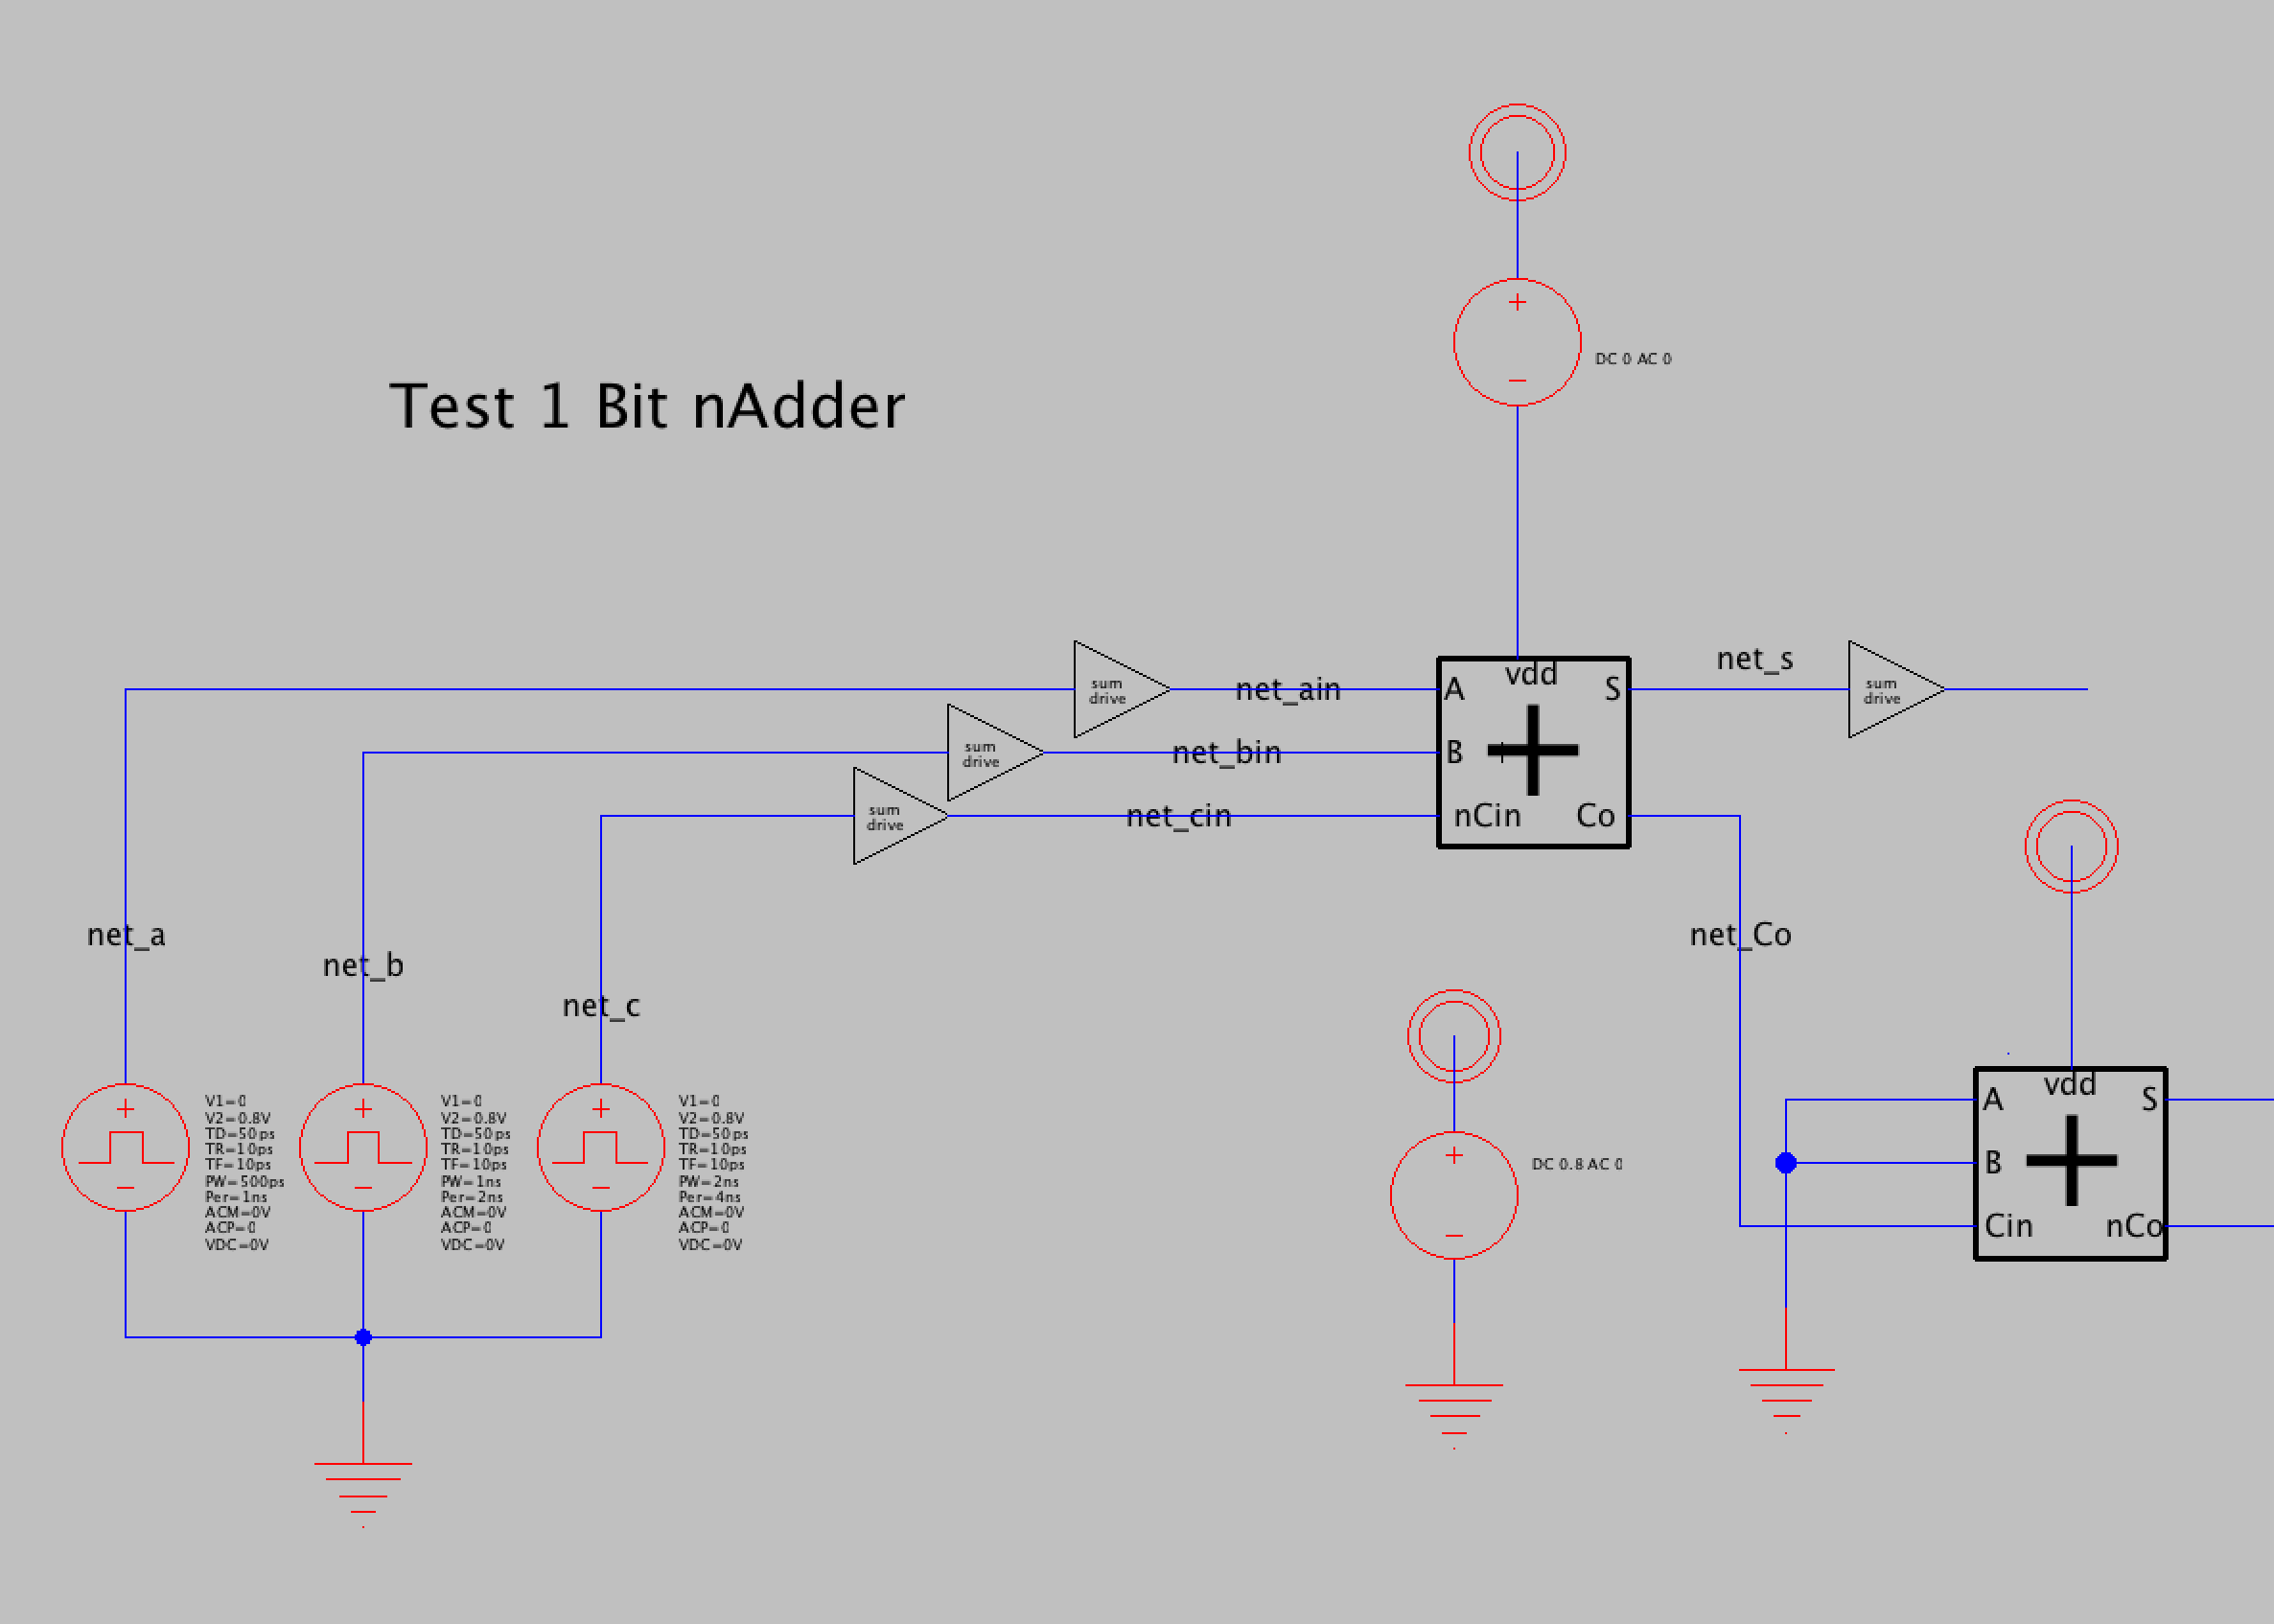
\includegraphics[width=\linewidth]{opt_screenshots/test_logic_1b_nadder_sch.png}
  \caption{Schematic used to test logical correctness of the 1-bit nAdder}
  \label{fig:test_logic_1b_nadder_sch}
\end{figure}

\begin{figure}[H]
  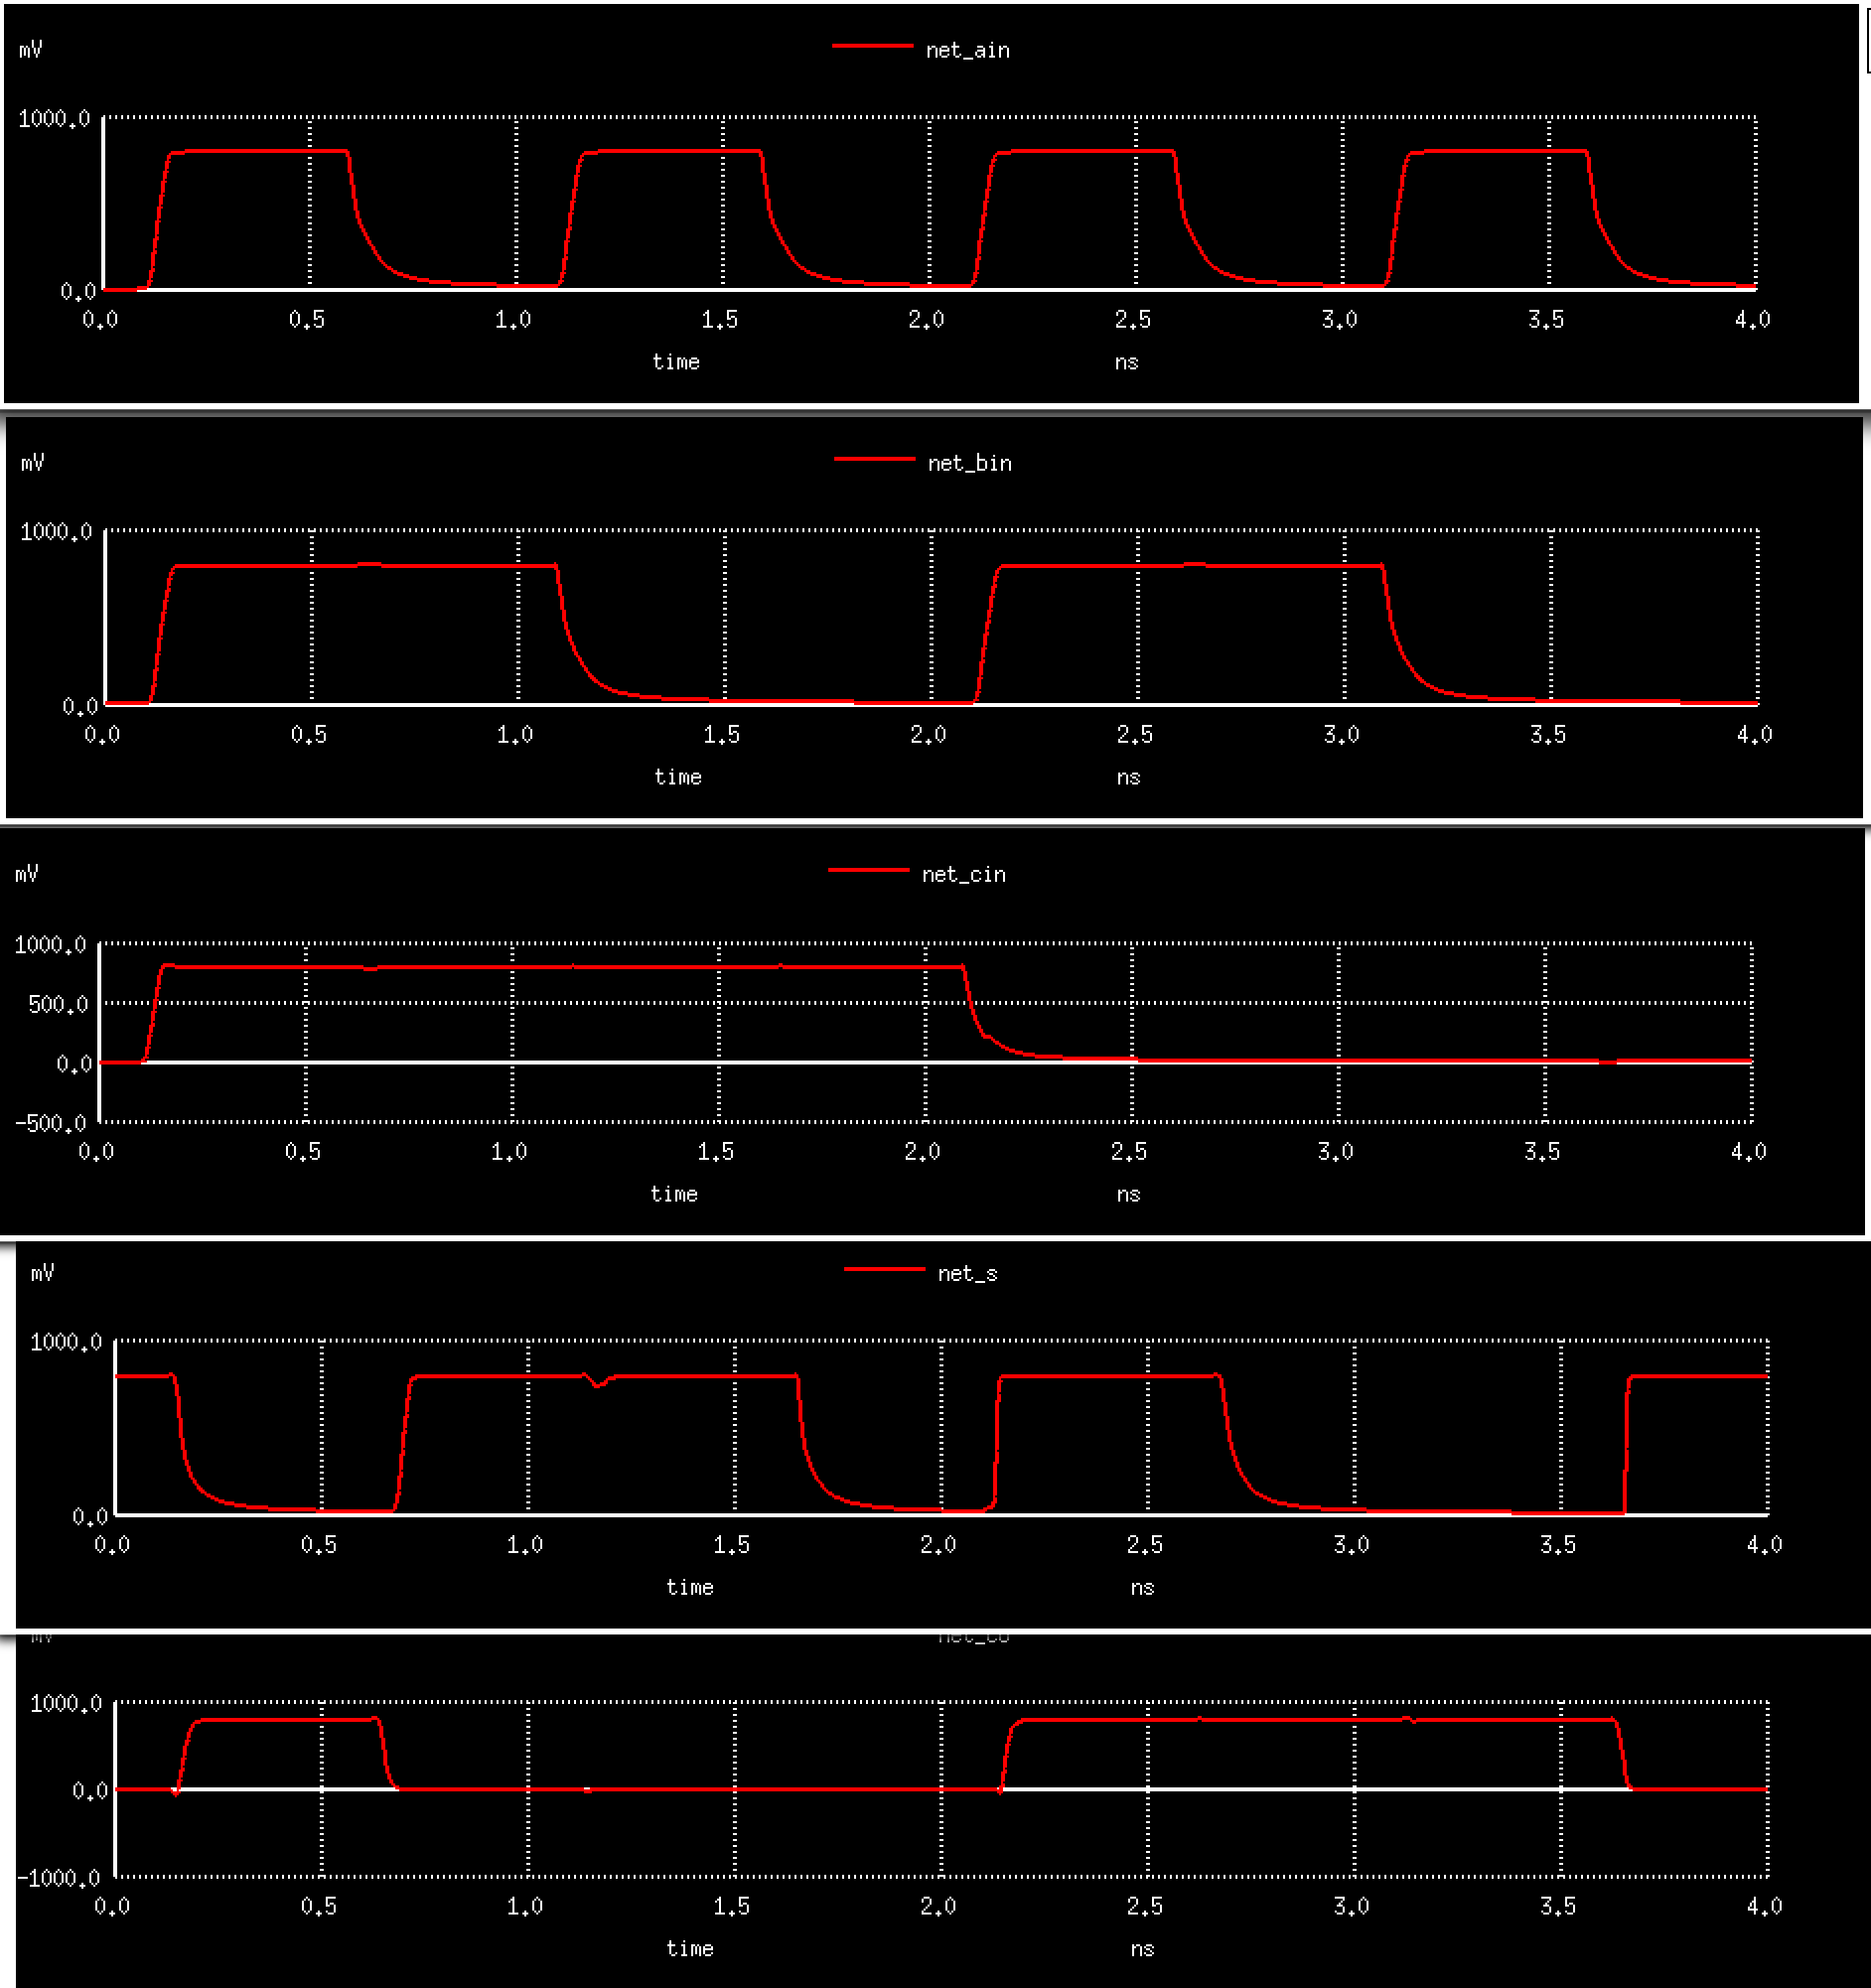
\includegraphics[width=\linewidth]{opt_screenshots/test_logic_1b_nadder.png}
  \caption{Waveform showing logical correctness of the 1-bit nAdder}
  \label{fig:test_logic_1b_nadder}
\end{figure}

\subsubsection{16-bit Adder}
To test the logical correctness of the 16-bit adder, I used the inputs $(A, B) = (0xffff, 0xffff) \rightarrow (0x0000, 0xffff) \rightarrow (0xffff, 0x0000) \rightarrow (0x0000, 0x0000)$. The important cases for correctness are the last three, which should have all sums as output $V_{dd}$, $V_{dd}$, and $0$ respectively. Those can be clearly seen from the simulation below in Figure \ref{fig:test_logic_16b_adder}.

\begin{figure}[H]
  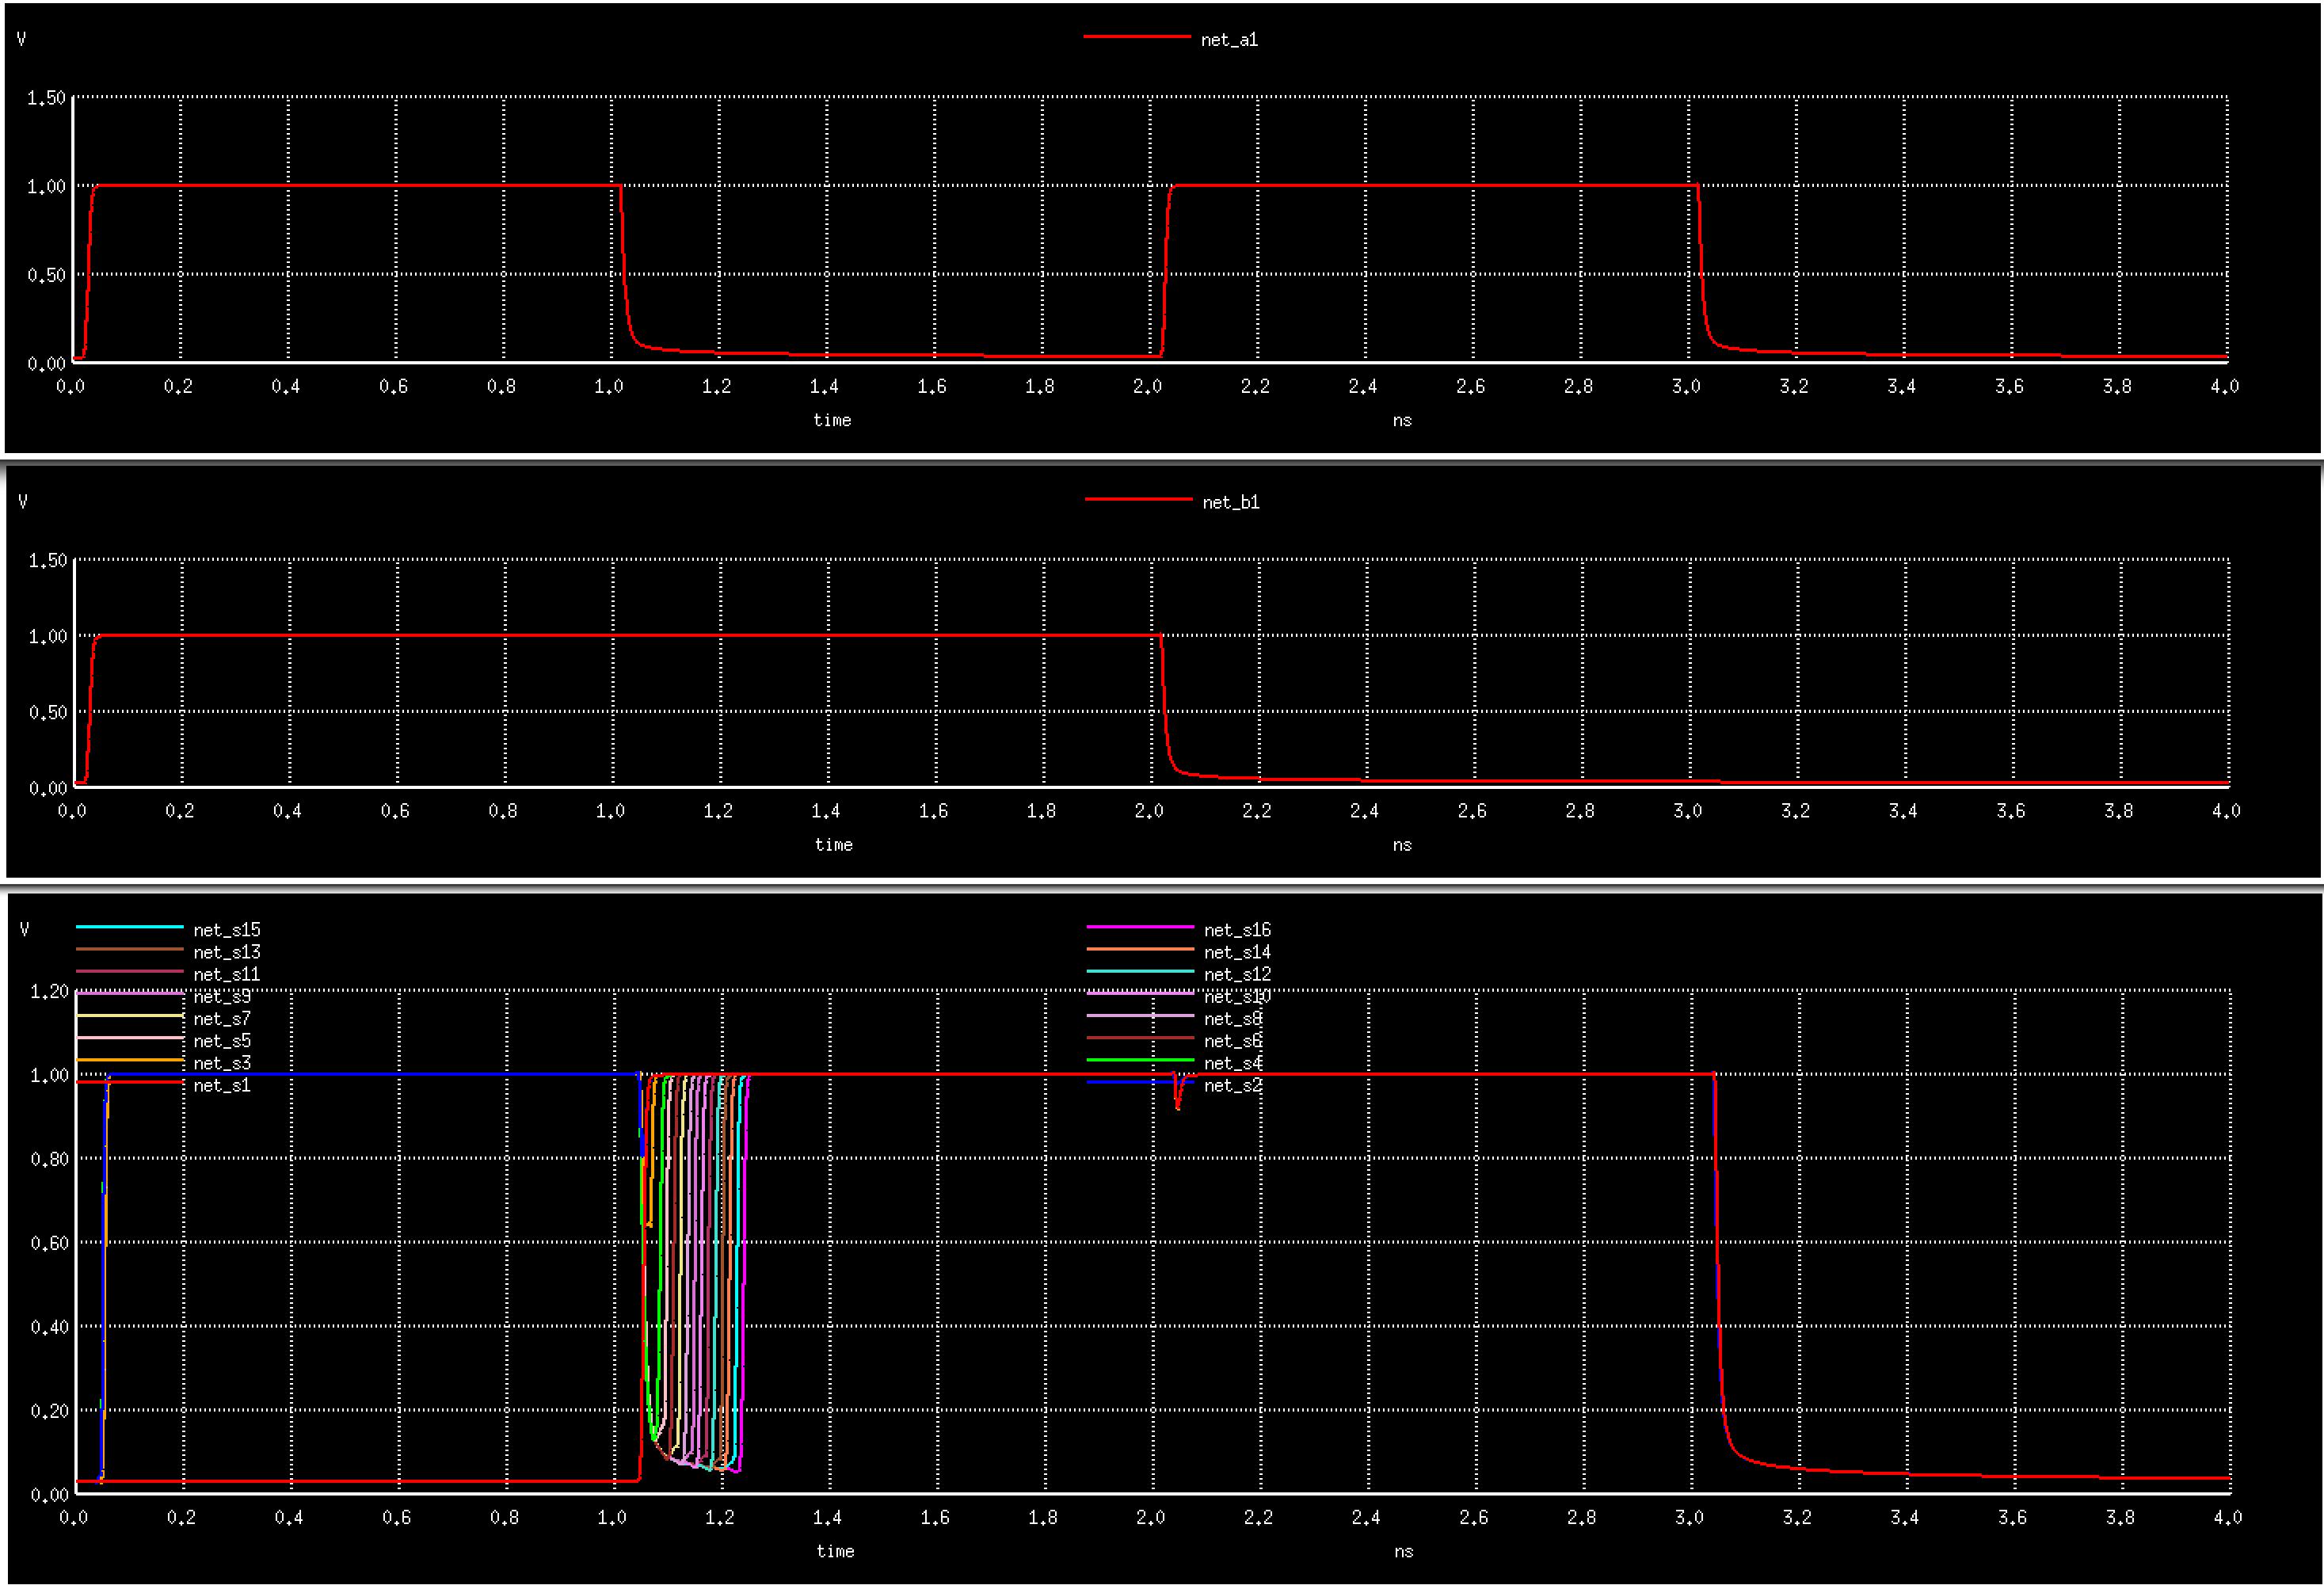
\includegraphics[width=\linewidth]{opt_screenshots/test_logic_16b_adder.png}
  \caption{Waveform showing logical correctness of the 1-bit nAdder}
  \label{fig:test_logic_16b_adder}
\end{figure}

\subsection{Delay}
\subsubsection{$\tau$ Approximation}

\subsubsection*{Sum}
\begin{align*}
d_{Sum} &= d_{XOR} + d_{XNOR} + d_{inv}\\
d_{XOR} &= max(d_{XOR(A,B) = (0, 1)}, d_{XOR(A,B) = (1, 0)})\\
d_{XNOR} &= max(d_{XNOR(A,B) = (1, 1)}, d_{XNOR(A,B) = (0, 0)})\\
\\
\textbf{for $XOR_{(A,B) = (1, 0)}$}\\
d_{XOR(A,B) = (1, 0)} &= R_{op}(C_{diff} + C_{g}) + R_{op}(C_{diff}) + (R_{op} + R_{on})(C_{diff} + 2C_g)\\
&\textnormal{Assume $R_{op} = R_{on} = R_{0}$}\\
&= R_{0}(C_{diff} + C_{g}) + R_{0}(C_{diff}) + (R_{0} + R_{0})(C_{diff} + 2C_g)\\
&\textnormal{Assume $\frac{C_{diff}}{\gamma} = C_{g} = C_{0}$}\\
&= R_{0}(\gamma C_{0} + C_{0}) + R_{0}(\gamma C_{0}) + (R_{0} + R_{0})(\gamma C_{0} + 2C_g)\\
&= R_{0}\gamma C_{0} + R_{0}C_{0} + R_{0}\gamma C_{0} + 2R_{0}\gamma C_{0} + 2R_{0}2C_g\\
&= (6 + 3\gamma)\tau\\
\\
&\textbf{for $XOR_{(A,B) = (0, 1)}$}\\
d_{XOR(A,B) = (0, 1)} &= R_{op}(C_{diff} + 2C_g) + (R_{op} + R_{on})(C_{diff} + 2C_g)\\
&\textnormal{Assume $R_{op} = R_{on} = R_{0}$}\\
&= R_{0}(C_{diff} + 2C_g) + (2R_{0})(C_{diff} + 2C_g)\\
&\textnormal{Assume $\frac{C_{diff}}{\gamma} = C_{g} = C_{0}$}\\
&= R_{0}(\gamma C_0 + 2C_0) + (2R_{0})(\gamma C_0 + 2C_0)\\
&= R_{0} \gamma C_0 + R_{0} 2 C_0 + 2R_{0}\gamma C_0 + 2 R_{0} 2C_0\\
&= \gamma \tau + 2\tau + 2\gamma\tau + 4\tau \\
&= 3\gamma\tau + 6\tau\\
&= (6 + 3\gamma)\tau\\
d_{XOR} &= max(d_{XOR(A,B) = (0, 1)}, d_{XOR(A,B) = (1, 0)})\\
&= (6 + 3\gamma)\tau\\
\\
d_{XOR} &= max(d_{XOR(A,B) = (0, 1)}, d_{XOR(A,B) = (1, 0)})\\
&= max((6 + 3\gamma)\tau, (6 + 3\gamma)\tau)\\
&= (6 + 3\gamma)\tau\\
\\
\\
\textbf{for $XNOR_{(A,B) = (1, 1)}$}\\
d_{XOR(A,B) = (1, 1)} &= R_{op}(C_{diff}) + (R_{op} + R_{on})(C_{diff} + 2C_{g})\\
&\textnormal{Assume $R_{op} = R_{on} = R_{0}$}\\
&= R_{0}(C_{diff}) + (2R_{0})(C_{diff} + 2C_{g})\\
&\textnormal{Assume $\frac{C_{diff}}{\gamma} = C_{g} = C_{0}$}\\
&= R_{0}(\gamma C_0) + (2R_{0})(\gamma C_{0} + 2C_{0})\\
&= \gamma\tau + 2\gamma\tau + 2\tau\\
&= (2 + 3\gamma)\tau
\\
\textbf{for $XOR_{(A,B) = (0, 0)}$}\\
d_{XOR(A,B) = (0, 0)} &= R_{op}(C_{diff} + C_g) + R_{op}(C_{diff} + 2C_g) + (R_{op} + R{on})(C_{diff} + 2C_g)\\
&\textnormal{Assume $R_{op} = R_{on} = R_{0}$}\\
&= R_{0}(C_{diff} + C_g) + R_{0}(C_{diff} + 2C_g) + 2R_{0}(C_{diff} + 2C_g)\\
&\textnormal{Assume $\frac{C_{diff}}{\gamma} = C_{g} = C_{0}$}\\
&= R_{0}(\gamma C_{0} + C_0) + R_{0}(\gamma C_{0} + 2C_0) + 2R_{0}(\gamma C_{0} + 2C_0)\\
&= R_{0}\gamma C_{0} + R_{0}C_0 + R_{0}\gamma C_{0} + R_{0}2C_0 + 2R_{0}\gamma C_{0} + 2R_{0}2C_0\\
&= \gamma\tau + \tau + \gamma\tau + 2\tau + 2\gamma\tau + 4\tau\\
&= (7 + 4\gamma)\tau\\
\\
d_{XNOR} &= max(d_{XNOR(A,B) = (1, 1)}, d_{XNOR(A,B) = (0, 0)})\\
&= max((2 + 3\gamma)\tau, (7 + 4\gamma)\tau)\\
&= (7 + 4\gamma)\tau
\\
\\
d_{inv} &= R_{op}(3C_g) = 3\tau\\
\\
\\
d_{Sum} &= d_{XOR} + d_{XNOR} + d_{inv}\\
&= (6 + 3\gamma)\tau + (7 + 4\gamma)\tau + 3\tau\\
&= (16 + 7\gamma)\tau
\end{align*}

\subsubsection*{nSum}
\begin{align*}
d_{nSum} &= d_{XOR} + d_{XOR} + d_{inv}\\
&= (6 + 3\gamma)\tau + (6 + 3\gamma)\tau + 3\tau\\
&= (15 + 6\gamma)\tau
\end{align*}

\subsubsection*{Carry}
\begin{align*}
d_{Carry} &= \frac{R_{op}}{2} + R_{op} \frac{R_{op}}{3})(4C_g)\\
&= \frac{22\tau}{3}\\
&\approx 7.33\tau
\end{align*}

\subsubsection*{nCarry}
\begin{align*}
d_{nCarry} &= \frac{3R_{op}}{6} + R_{op} \frac{2R_{op}}{6})(4C_g)\\
&= \frac{22\tau}{3}\\
&\approx 7.33\tau
\end{align*}


\subsubsection*{1-bit Adder}
\begin{align*}
d_{1bAdder} &= d_{buffer} + max(d_{Sum}, d_{Carry})\\
&= 6\tau max((16 + 7\gamma)\tau, 7.33\tau)\\
&= (22 + 7\gamma)\tau
\end{align*}

\subsubsection*{1-bit nAdder}
\begin{align*}
d_{1bnAdder} &= max(d_{nSum}, d_{nCarry})\\
&= max((15 + 6\gamma)\tau, 7.33\tau)
\end{align*}

\subsubsection*{16-bit Adder}
\begin{align*}
d_{16bAdder} &= 15d_{Carry} + d_{Sum}\\
&= 15(\frac{22\tau}{3}) + (16 + 7\gamma)\tau\\
&= (126 + 7\gamma)\tau
\end{align*}

\subsubsection{Measuring $\tau$}
To measure $\tau$, I used the FO4 topology (Figure \ref{fig:inv_fo4_sch}) with a minimum-sized inverter. This topology should give delay of $R_0 \times 8C_0 = 8\tau$. After simulation (Figure \ref{fig:inv_fo4_sim}), I found $8\tau = 4.21505\times 10^{-12} = 526.881fs$.

\begin{figure}[H]
  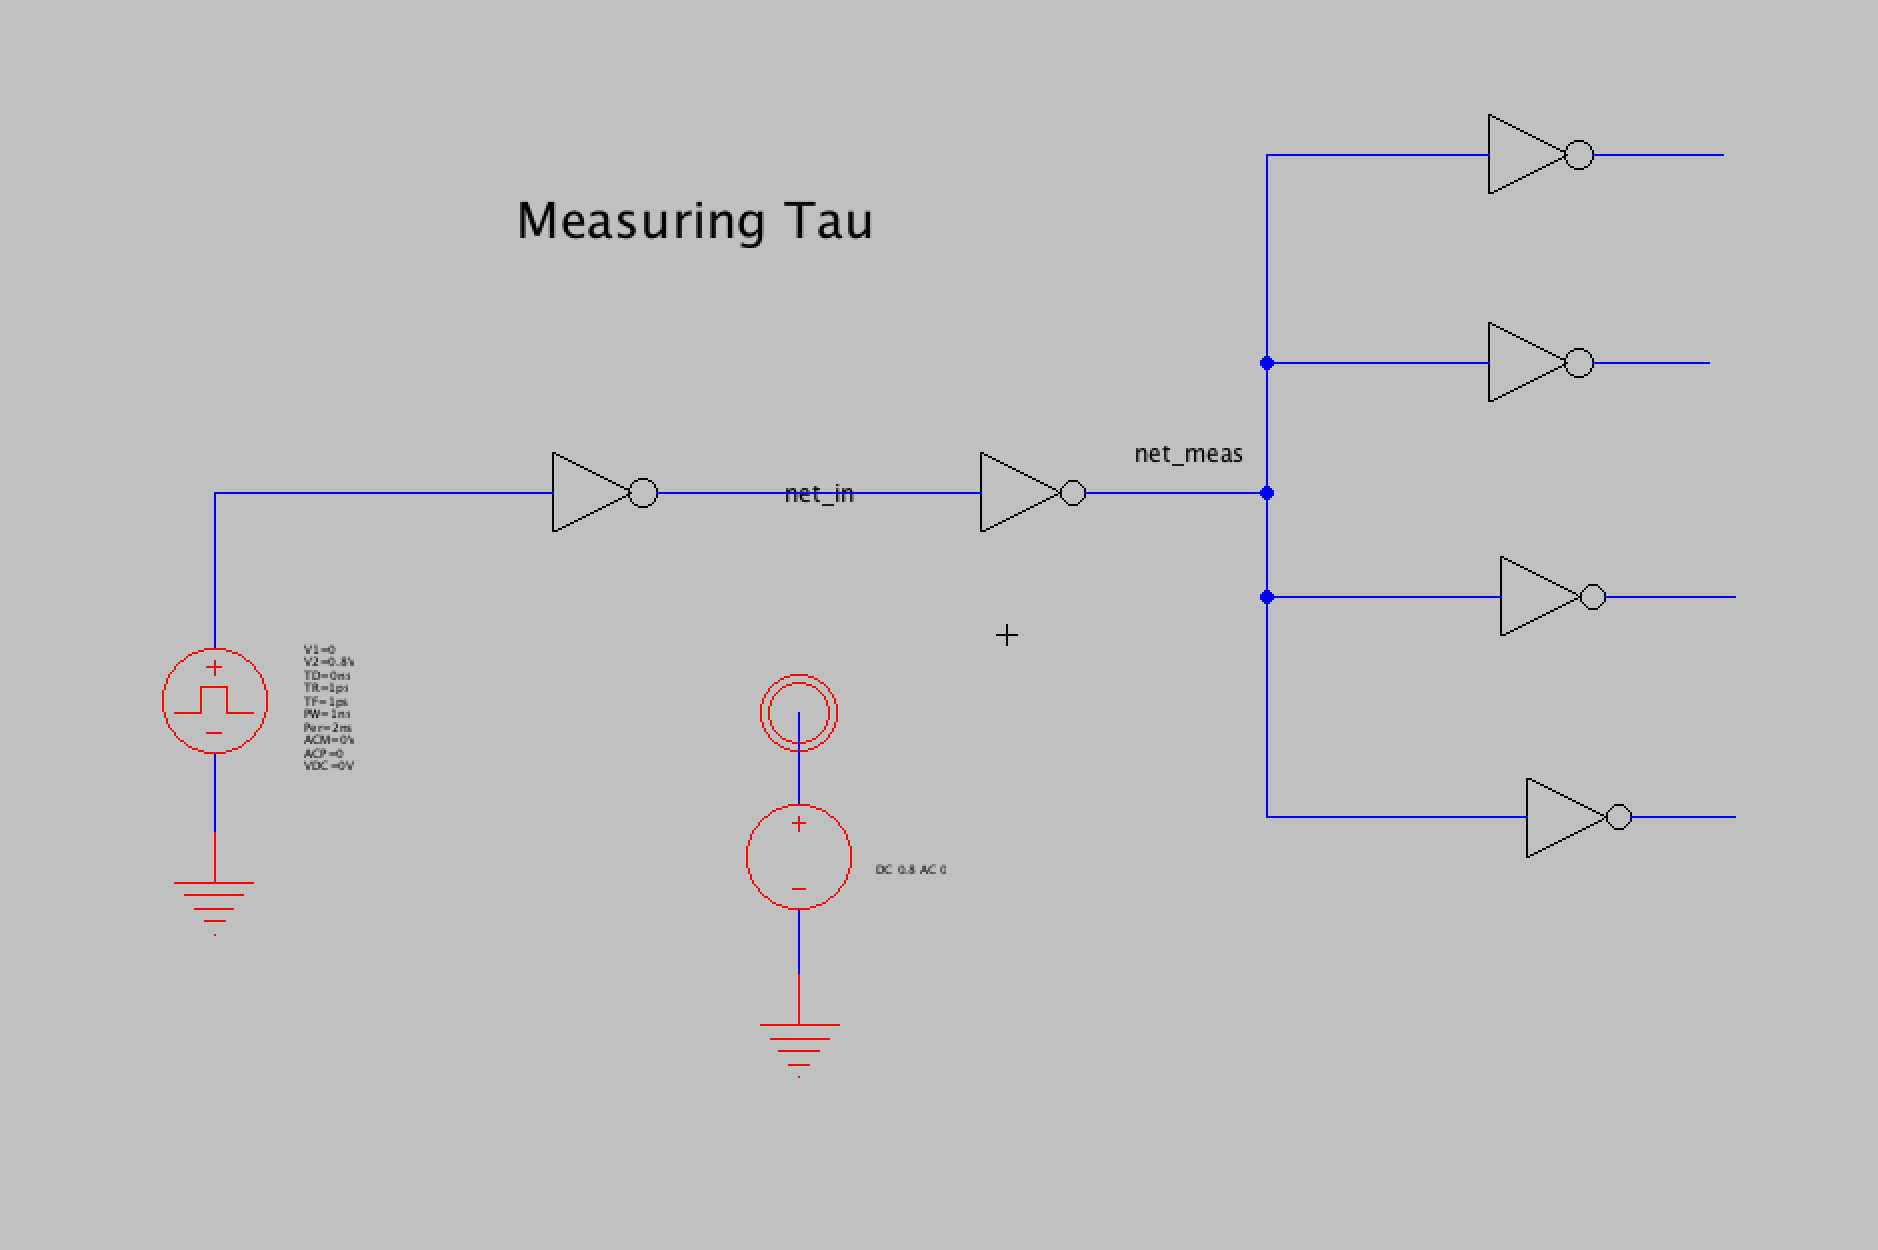
\includegraphics[width=\linewidth]{opt_screenshots/inv_fo4_sch.png}
  \caption{FO4 inverter topology for measuring $\tau$}
  \label{fig:inv_fo4_sch}
\end{figure}

\begin{figure}[H]
  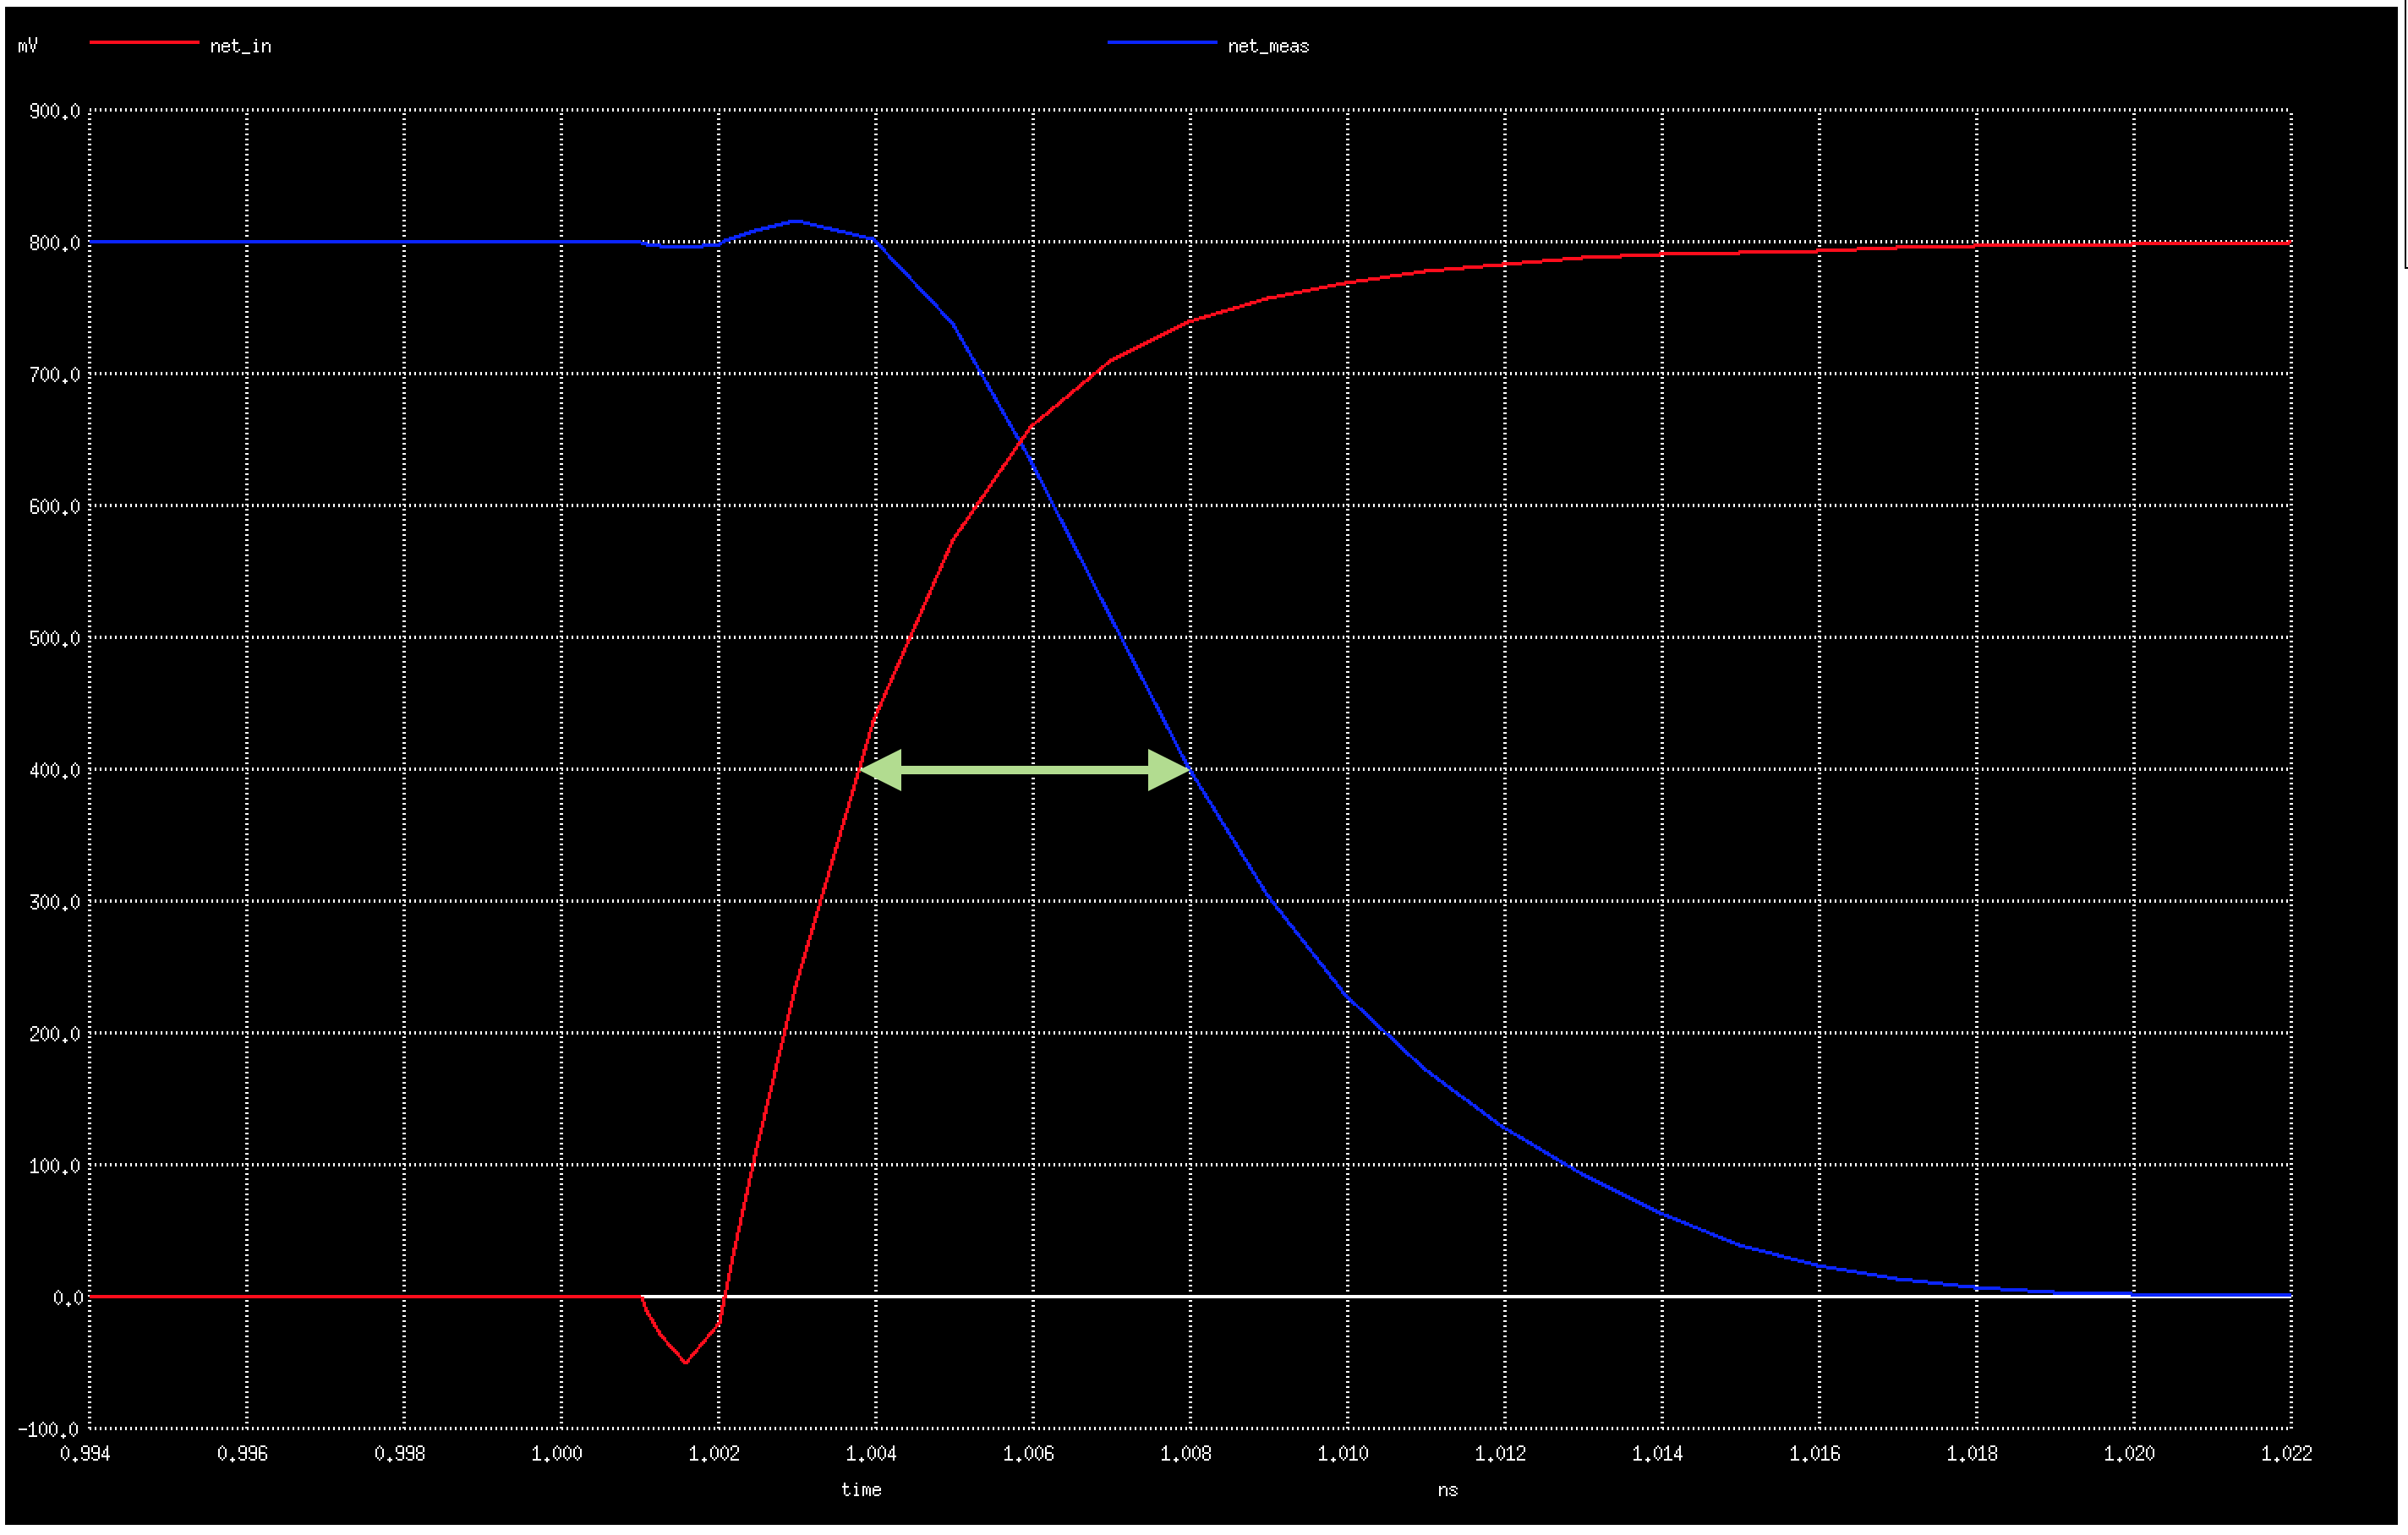
\includegraphics[width=\linewidth]{opt_screenshots/inv_fo4_sim.png}
  \caption{Simulation of FO4 inverter output}
  \label{fig:inv_fo4_sim}
\end{figure}

\subsubsection{Measuring 16-bit Adder Delay}
The delay from the 16-bit adder was measured with inputs $(A, B) = (0xffff, 0x0000) \rightarrow (0xffff, 0x0001)$. This is because the propagation delay for the carry through the entire 16-bit adder takes longest when the carry must be propagated through all 16 adders. The last node to charge on the output is the sum output of the 16th adder because the input capacitance of the sum gate. Each set of 1-bit adder inputs is driven with a buffer made from the 1-bit adder, and they are loaded with the same 1-bit adder buffer (Figure \ref{fig:opt_adder_buffer_sch}). The final two outputs are the 16th 1-bit adder sum and 16th 1-bit adder carry out. Those simulated waveforms are below in Figure \ref{fig:opt_16b_adder_delay_waveform} and Figure \ref{fig:opt_16b_adder_delay_waveform}. The delay is $211.463ps$.

\begin{figure}[H]
  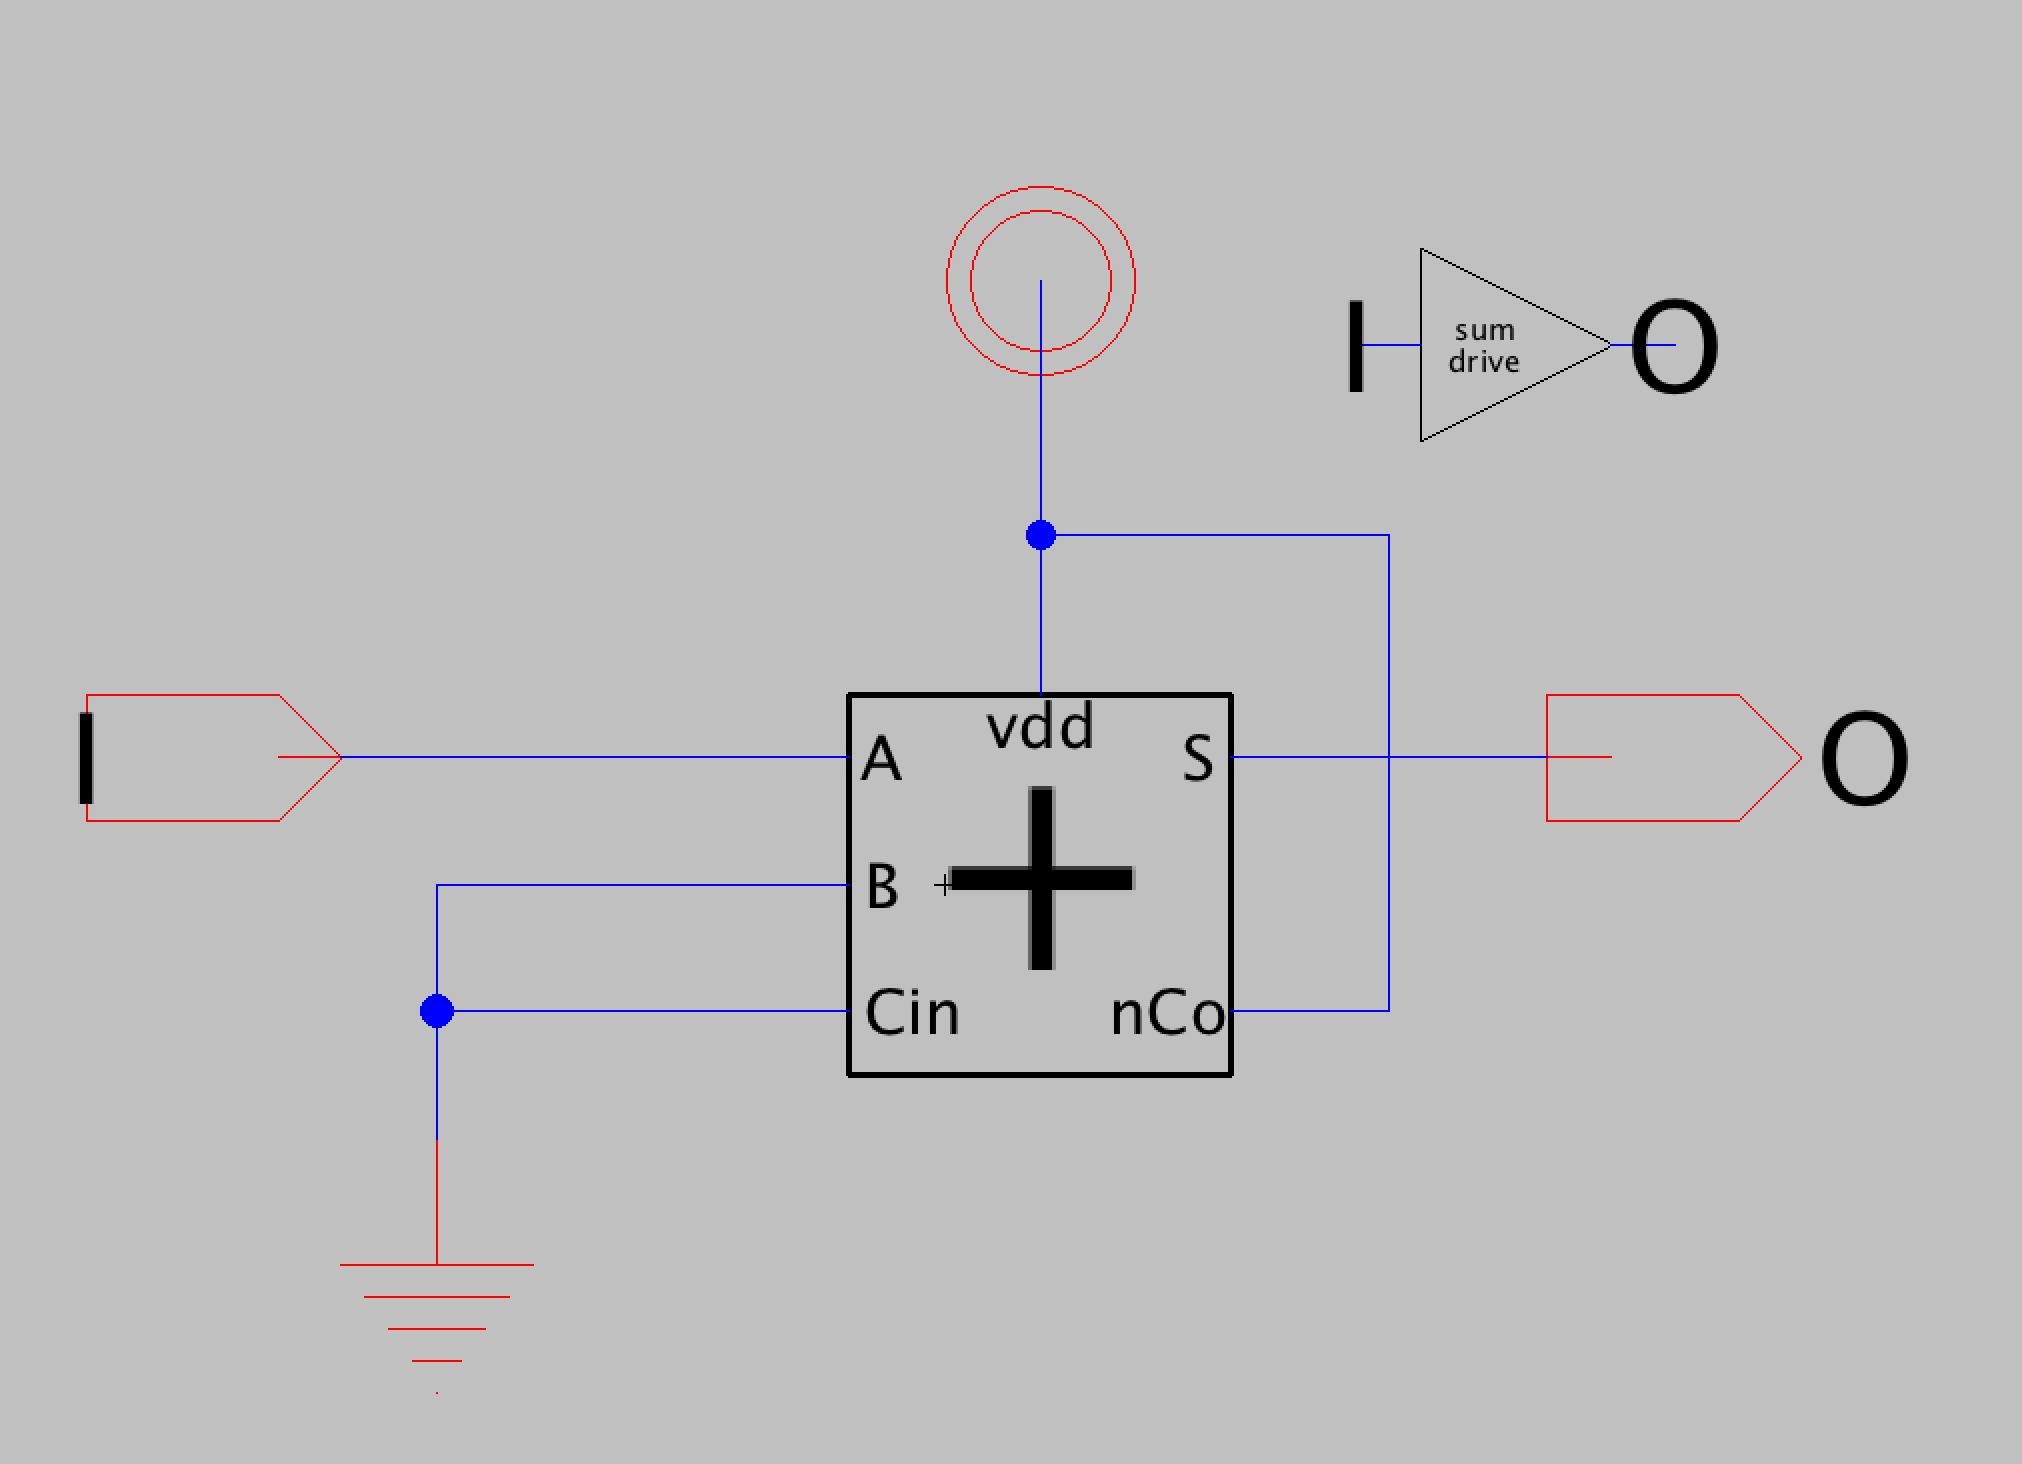
\includegraphics[width=\linewidth]{opt_screenshots/opt_adder_buffer_sch.png}
  \caption{Buffer for Adder}
  \label{fig:opt_adder_buffer_sch}
\end{figure}

\begin{figure}[H]
  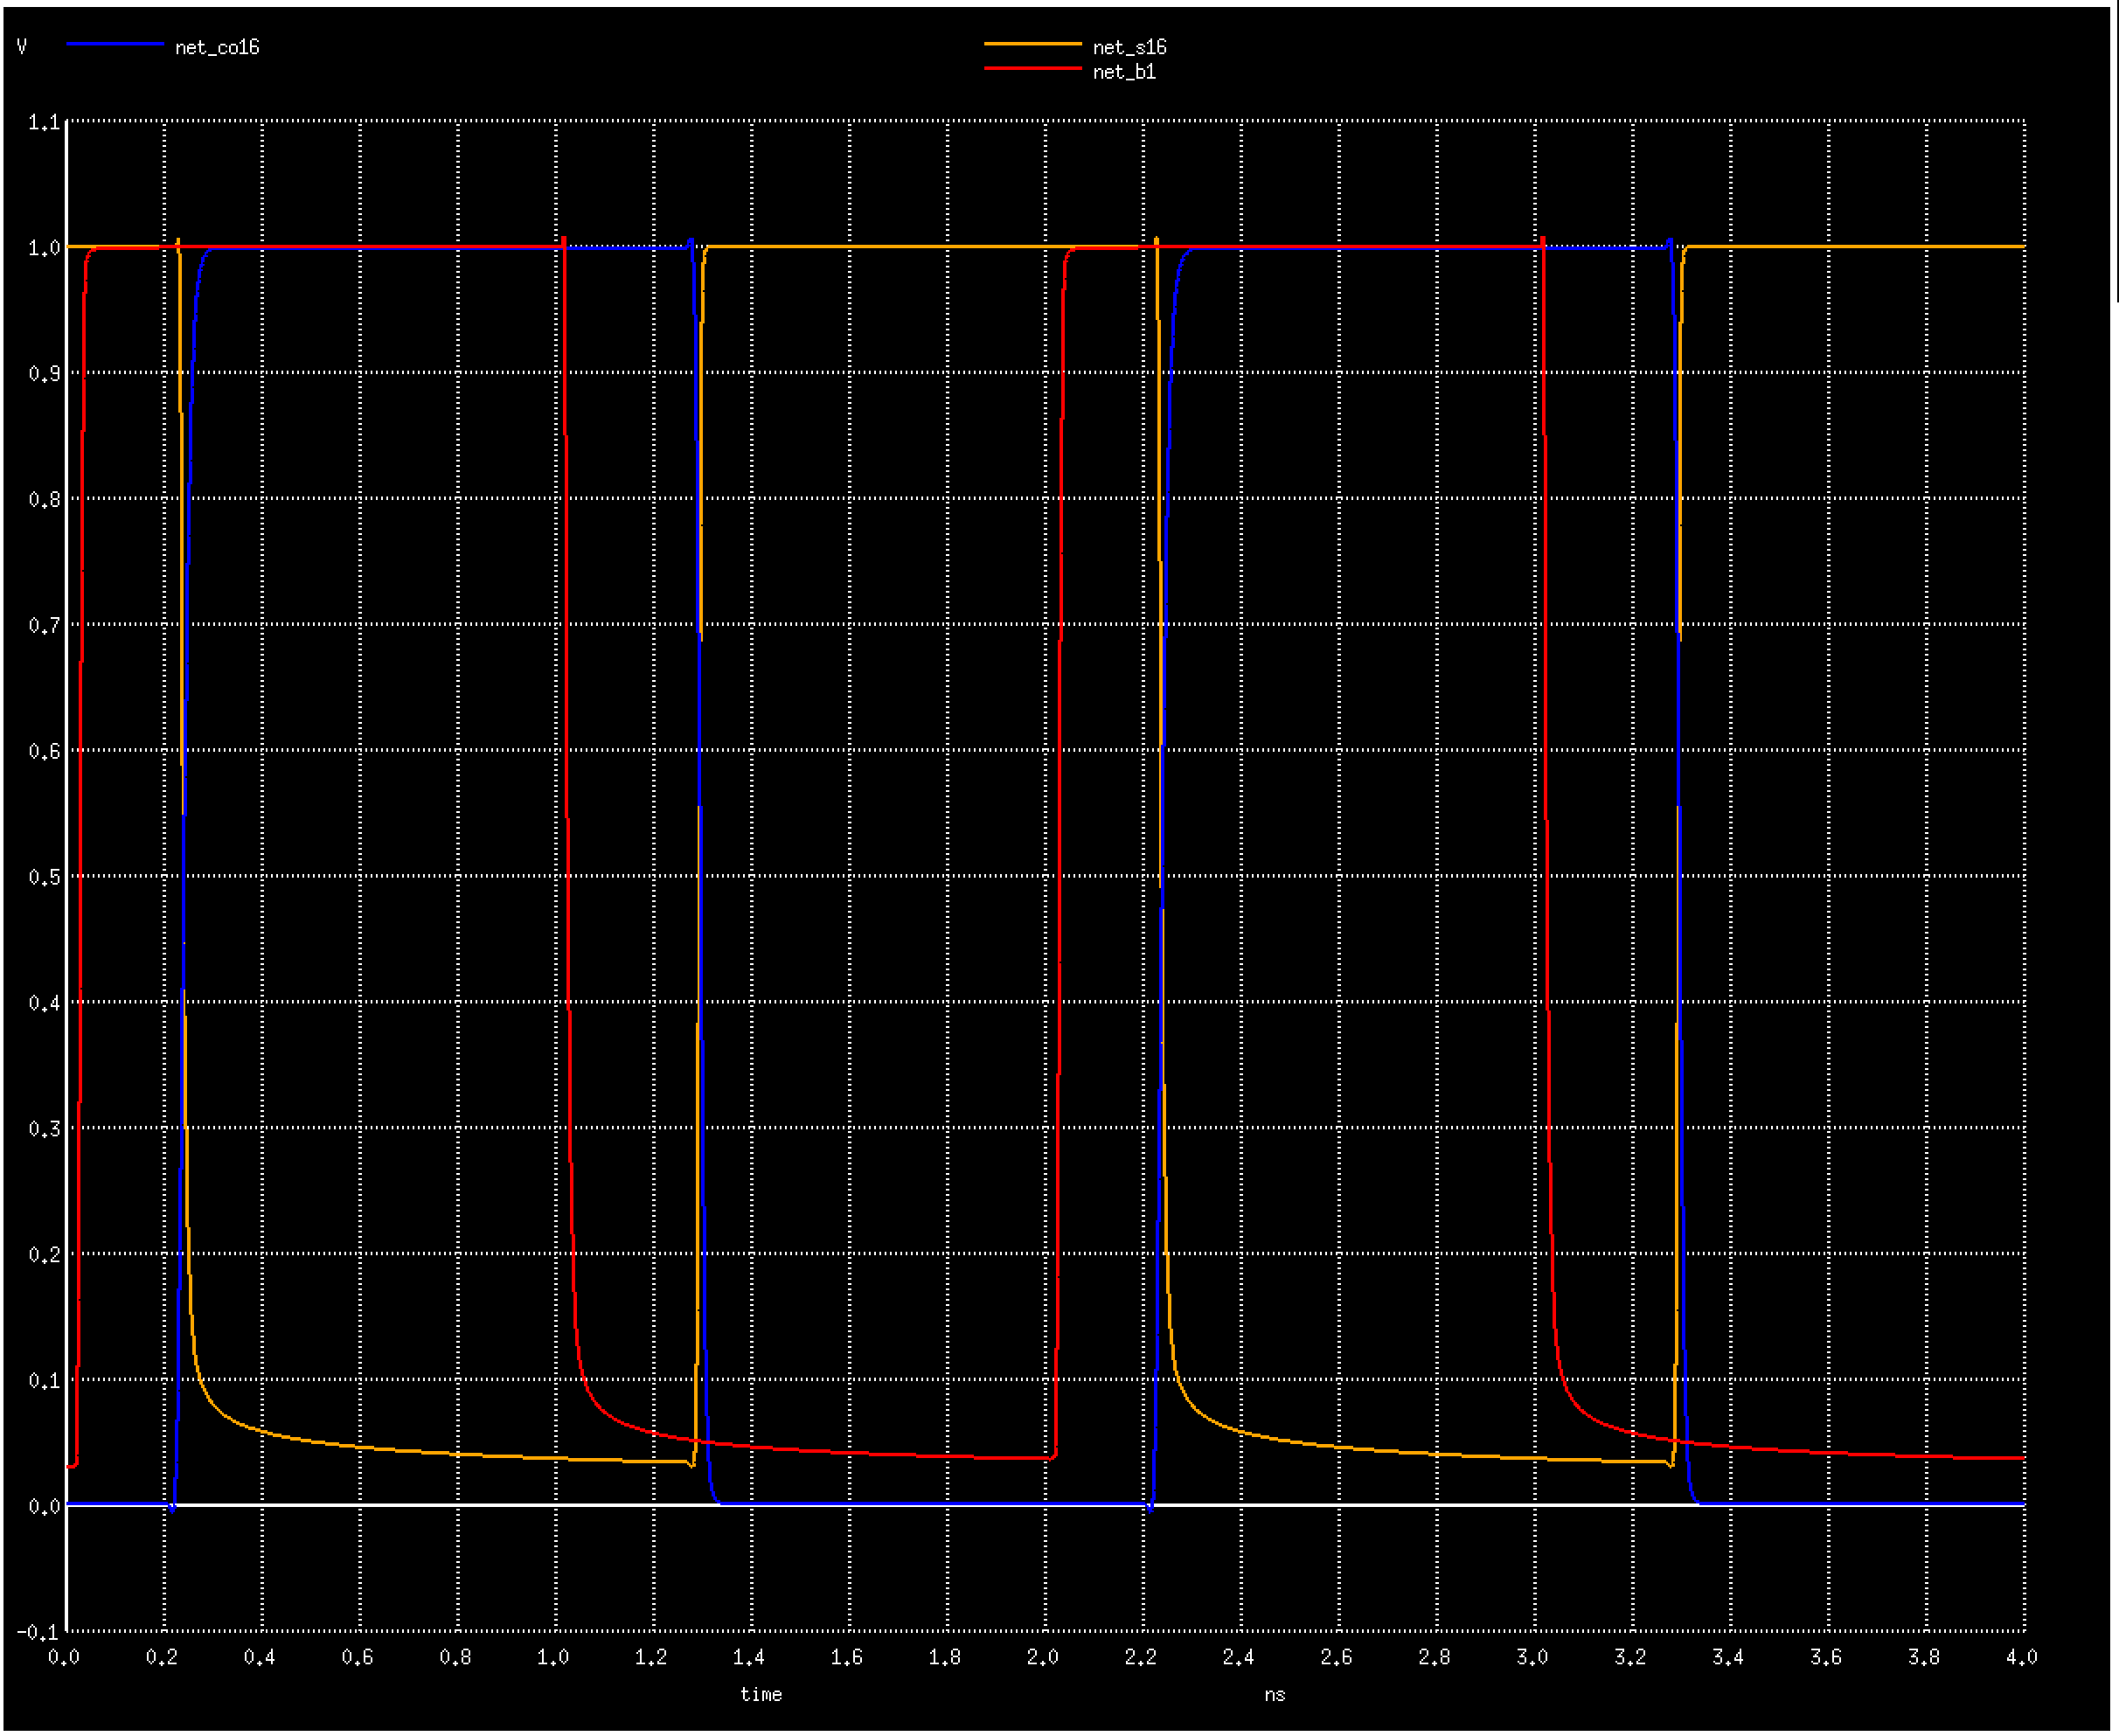
\includegraphics[width=\linewidth]{opt_screenshots/opt_16b_adder_delay_waveform.png}
  \caption{Simulation of 16-Bit adder}
  \label{fig:opt_16b_adder_delay_waveform}
\end{figure}

\begin{figure}[H]
  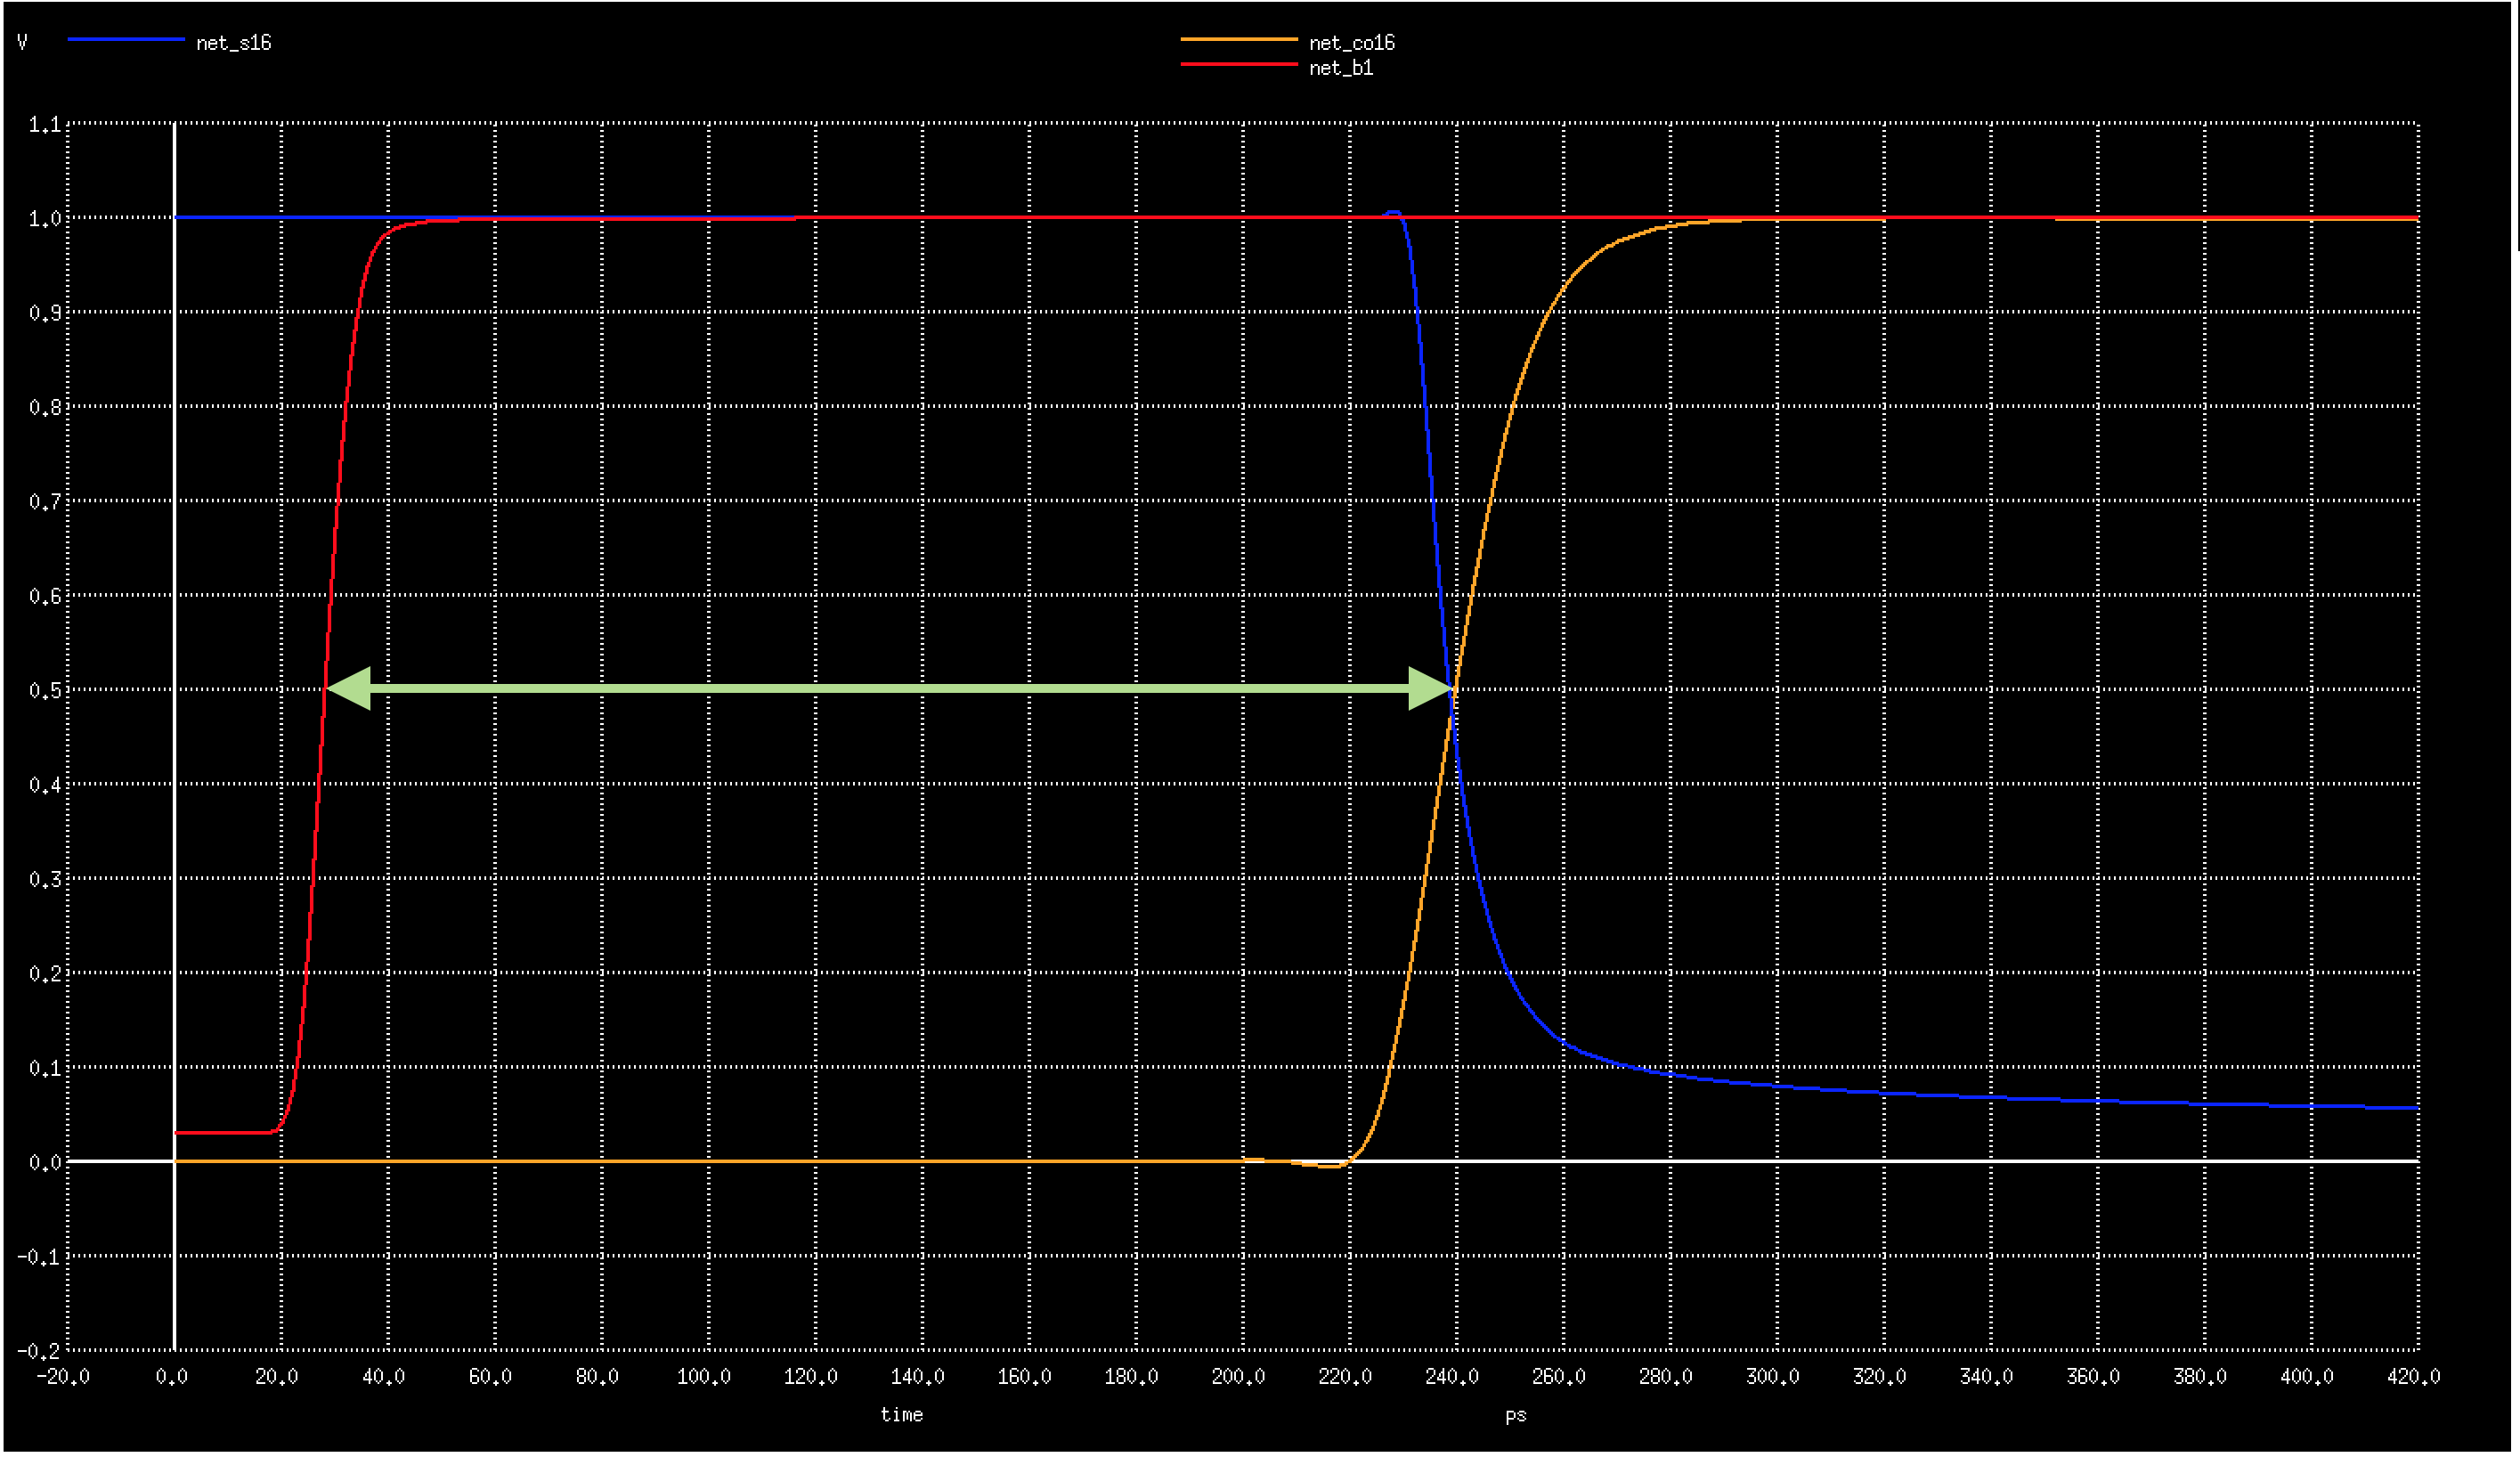
\includegraphics[width=\linewidth]{opt_screenshots/opt_16b_adder_delay_waveform_zoom.png}
  \caption{Simulation of 16-Bit adder showing delay}
  \label{fig:opt_16b_adder_delay_waveform_zoom}
\end{figure}

\subsubsection{Comparing Calculations with Simulation}
The calculated delay is $(126 + 7\gamma)\tau$. Let's make the assumption that $\gamma \approx 1.5$. therefore, we have a delay of $136.5\tau = 300.3 \times 0.5269 = 158.2ps$, which is less than the simulated delay of $211.463ps$, but is close considering I did not take into consideration the diffusion region capacitances for the carry modules. It is evident that models more complex than the $\tau$ model must be used to estimate the delay of this circuit. 

\subsection{Area}
The area is calculated with a minimum-sized transistor as 1 unit and a transistor of width 2 and length 1 is 2 units:
\begin{align*}
Area &= 8 \times A_{Adder} + 8 \times A_{nAdder}\\
A_{Adder} &= 12 + A_{Sum} + A_{Carry}\\
&= 12 + A_{XOR} + A_{XNOR} + 2 + 20\\
&= 12 + 8 + 8 + 2 + 20\\
&= 50units\\
A_{nAdder} &= A_{nSum} + A_{nCarry}\\
&= A_{XOR} + A_{XOR} + 2 + 28\\
&= 8 + 8 + 2 + 28\\
&= 46units\\
\\
Area &= 8 \times A_{Adder} + 8 \times A_{nAdder}\\
&= 8 \times 50 + 8 \times 46\\
&= 768units
\end{align*}

\subsection{Energy}
\subsubsection{Leakage Energy}
To find maximum leakage energy input permutation, I used the same logic as for 1-bit Adder and nAdder since all inputs are accounted for. The graph of the current consumed by the Adder is in Figure \ref{fig:energy_adder_waveform}

\begin{figure}[H]
  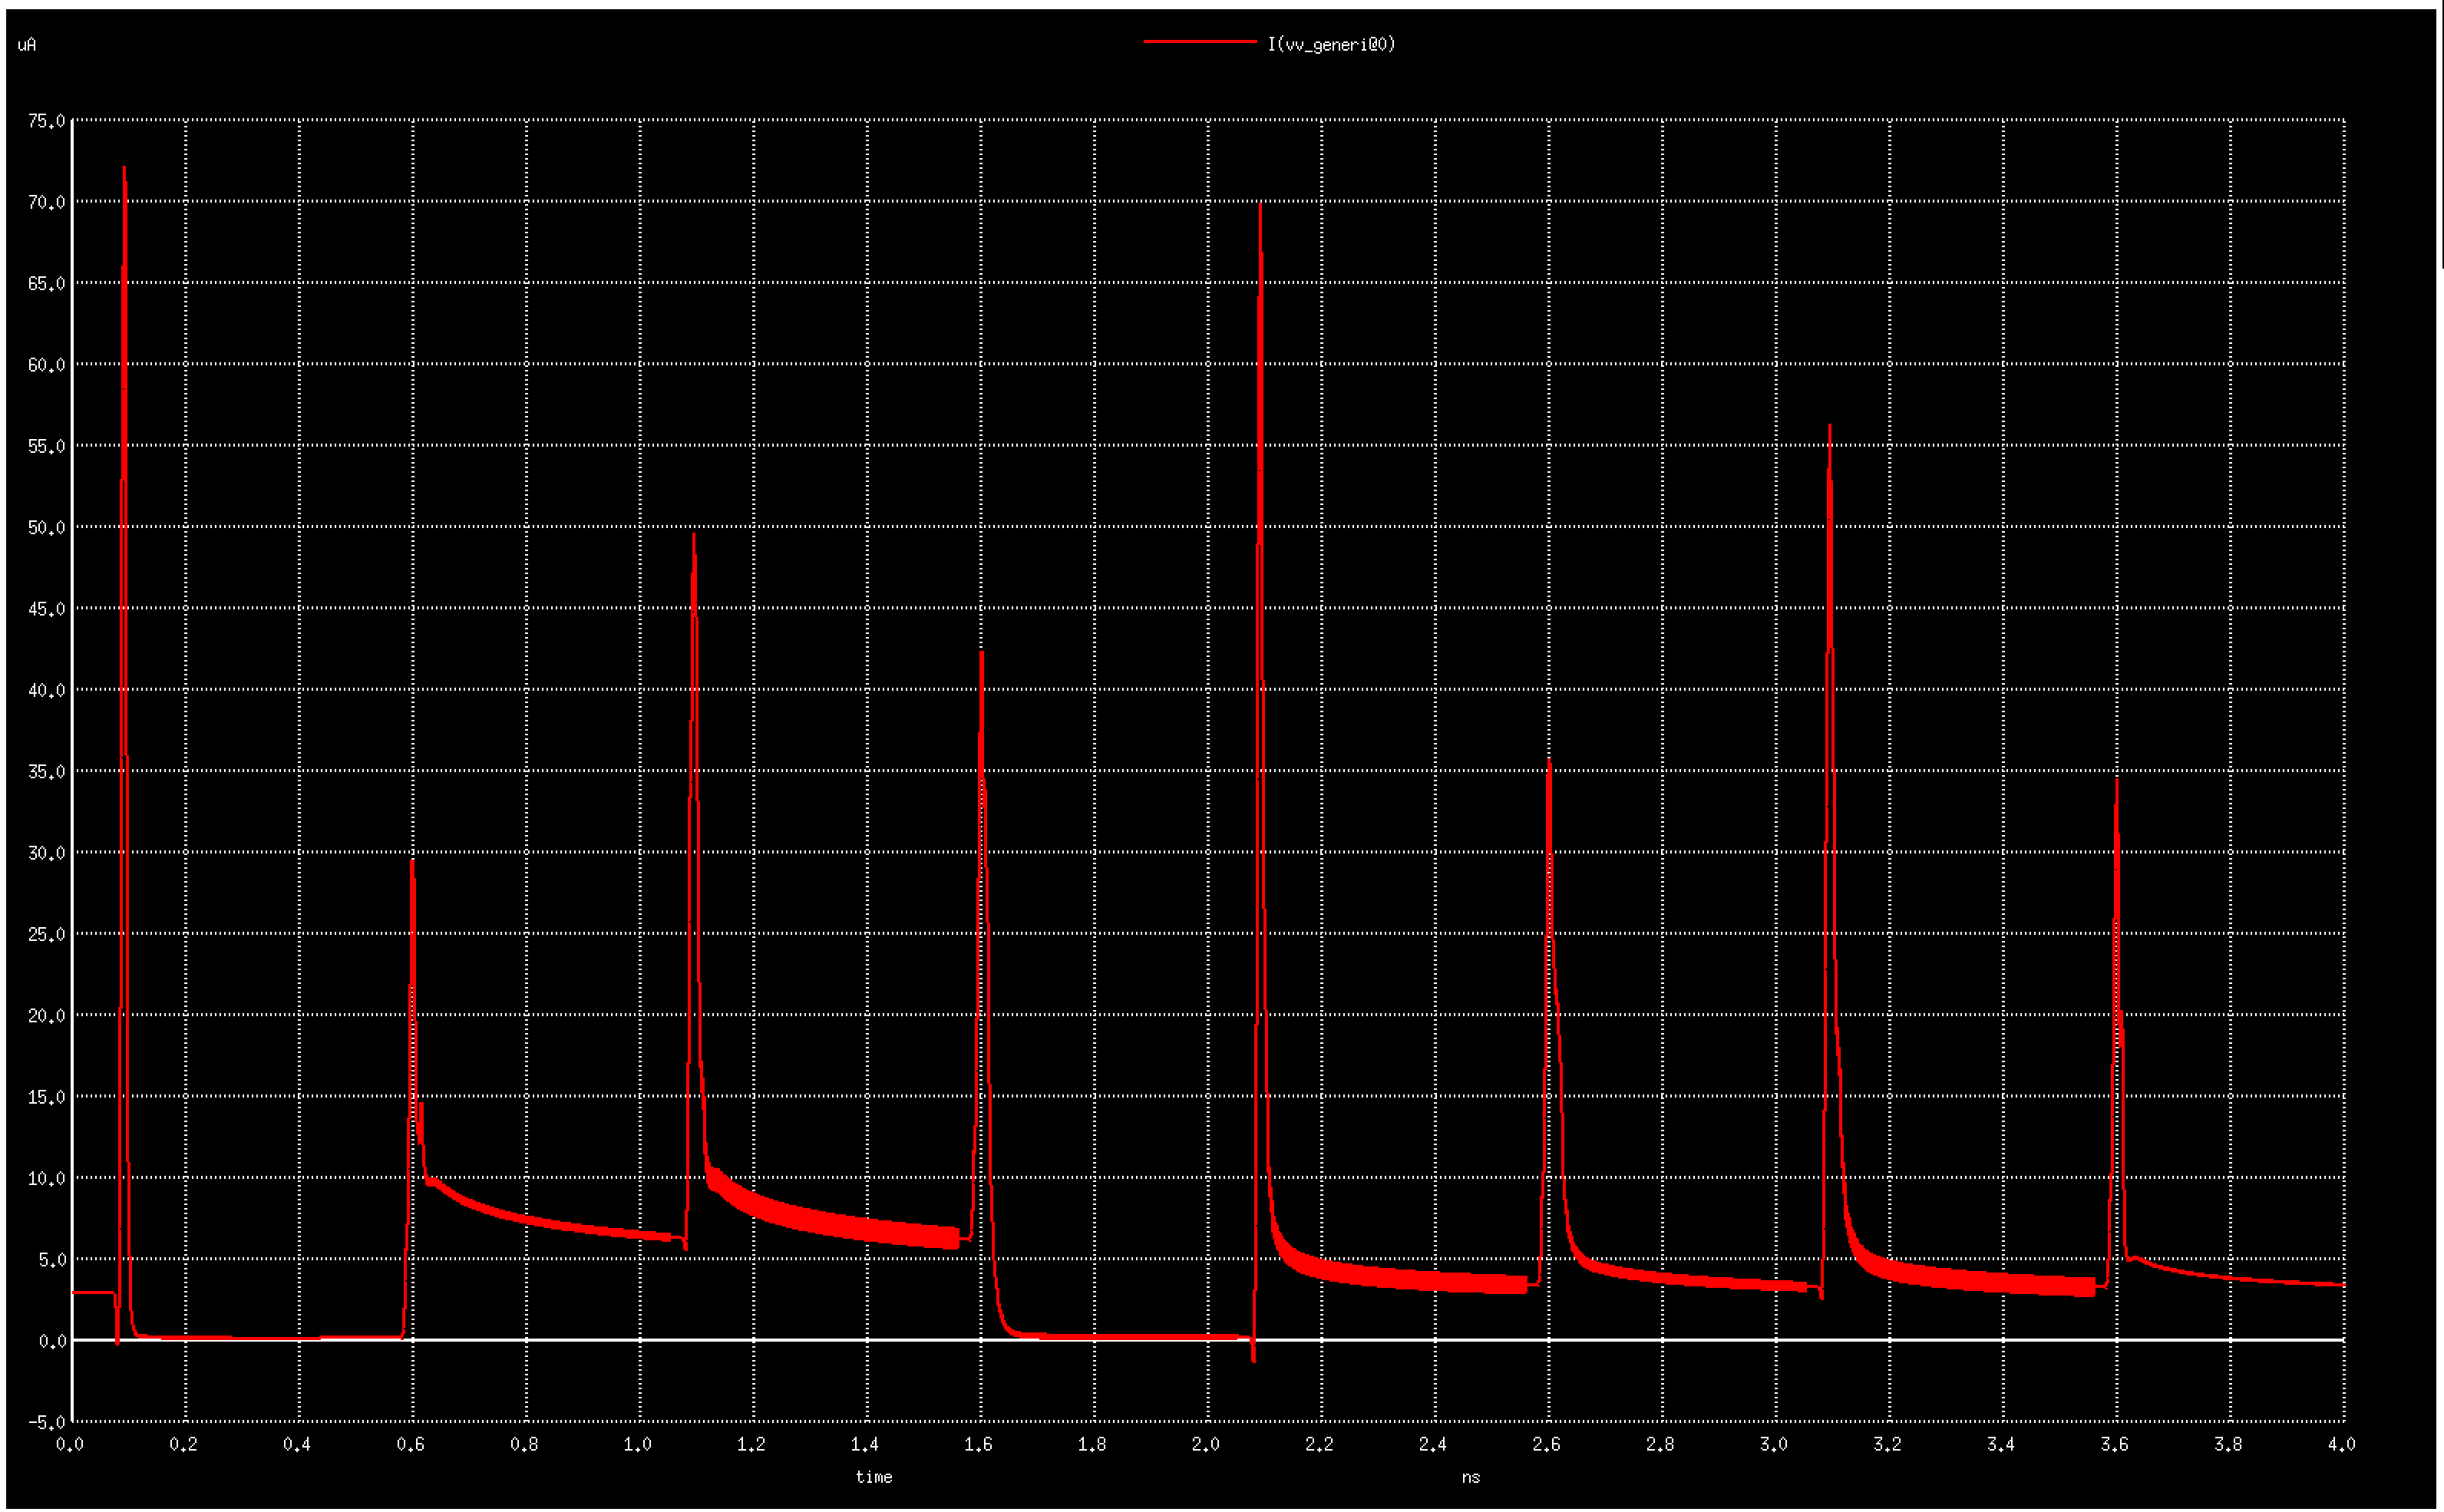
\includegraphics[width=\linewidth]{opt_screenshots/energy_adder_waveform.png}
  \caption{Simulation of the energy consumption of the 1-bit Adder}
  \label{fig:energy_adder_waveform}
\end{figure}

\subsubsection*{Maximum Case}
The maximum case occurs between $t = 1.2 \rightarrow 1.4ns$, which is the input case $(A, B, C) = (1,0,1)$ and using\\
\code{meas tran yint integ I(vv\_generi@0) from=1200ps to=1411ps}\\
we get $1.54217fW$. Each adder consumes this much energy, so we have $16 \times 1.54217fW = 24.67472fW$

\subsubsection*{Minimum Case}
The maximum case occurs in the interval $t = 0.2 \rightarrow 0.4ns$, which is the input case $(A, B, C) = (1,1,1)$ and using\\
\code{meas tran yint integ I(vv\_generi@0) from=200ps to=411ps}\\
we get $0.0388214fW$. Each adder also consumes this much minimum case leakage energy, so we have $16 \times 0.0388214fW = 0.6211424fW$. 

\subsubsection{Active Energy}

\subsubsection*{Maximum Case}
The maximum energy case is when all outputs must be charged by the minimum number of parallel transistors. This occurs when only 2 of the 3 inputs for the sum is on. That is $(A, B) = (0xffff, 0x0000 \rightarrow 0x0001)$ so the delay propagates. 
I used the following spice command:\\
\code{meas tran yint integ I(vv\_adder) from=0ps to=4ns}\\
The result is $268.364fW$. 

\subsubsection*{Average Case}
To calculate this, I use the four cases $(A, B) =  (0xffff, 0xffff) \rightarrow (0x0000, 0xffff) \rightarrow (0xffff, 0x0000) \rightarrow (0x0000, 0x0000) \rightarrow (0xffff, 0xffff)$ and divided the total energy consumed by 4, since we have 4 switching input cases. I used the following command: \\
\code{meas tran yint integ I(vv\_adder) from=0ps to=5ns}\\
The result is $\frac{236.575fW}{4} = 59.14375fW$. 
\section{Alternate Designs and Considerations}
As stated above, the following is the order in which I tried optimizations. 
\begin{enumerate}
\item Replace 3-input XOR with pass transistor logic XOR cascade ($667.123ps \rightarrow 528.022ps$)
\item Change $V_{dd} = 0.8V \rightarrow V_{dd} = 1V$ ($528.022ps \rightarrow 309.259ps$)
\item Re-order inputs to Carry and nCarry to reduce the $C_{diff}$ for the later input ($309.259ps \rightarrow 295.593ps$)
\item Increase width of transistors with $A$ and $B$ inputs for Carry and nCarry  ($295.593ps \rightarrow 274.925ps$)
\item Add step-up stages for $A$ and $B$ inputs for Carry and nCarry  ($274.925ps \rightarrow 280.286ps$)*
\item Add step-up stages for $A$ and $B$ inputs for 1-bit Adder  ($274.925ps \rightarrow 271.282ps$)
\item Add step-up stages for $A$ and $B$ inputs for 1-bit nAdder  ($271.282ps \rightarrow 271.864ps$)*
\end{enumerate}
The two alternate designs denoted with the * failed to improve timing. In both cases, the added delay created by the buffers outweighed the reduction in delay from reducing the input capacitance to the gate.\\
As part of the pass-transistor logic, I first attempted to create a non-cascaded version, making a single pass-transistor XOR3 gate. This, however created a large $Ron$, since there were 2 pass transistors in series, and it also had a non-minimal input capacitance.\\
The increase in $V_{dd}$ gave a sizable decrease in delay, much more than expected. The gain from input reordering was also more sizable than I originally expected. 

\section{Continuing Optimizations}
List of proposed further optimizations (other than those above):
\begin{enumerate}
\item explore cascaded CMOS topology for sum instead of pass transistor logic
\item ratioed logic
\item cascade gates to calculate carry out
\item manipulate transistor widths to equalize wost-case Ron in all stages
\item optimize number of stages for sum
\item equalize input capacitance on all inputs
\end{enumerate}

\section{Code of Academic Integrity}
I, Phillip Trent, certify that I have complied with the University of Pennsylvania’s Code of Academic Integrity in completing this project.
\end{document}


